\documentclass[twoside]{book}

% Packages required by doxygen
\usepackage{calc}
\usepackage{doxygen}
\usepackage{graphicx}
\usepackage[utf8]{inputenc}
\usepackage{makeidx}
\usepackage{multicol}
\usepackage{multirow}
\usepackage{textcomp}
\usepackage[table]{xcolor}

% Font selection
\usepackage[T1]{fontenc}
\usepackage{mathptmx}
\usepackage[scaled=.90]{helvet}
\usepackage{courier}
\usepackage{amssymb}
\usepackage{sectsty}
\renewcommand{\familydefault}{\sfdefault}
\allsectionsfont{%
  \fontseries{bc}\selectfont%
  \color{darkgray}%
}
\renewcommand{\DoxyLabelFont}{%
  \fontseries{bc}\selectfont%
  \color{darkgray}%
}

% Page & text layout
\usepackage{geometry}
\geometry{%
  a4paper,%
  top=2.5cm,%
  bottom=2.5cm,%
  left=2.5cm,%
  right=2.5cm%
}
\tolerance=750
\hfuzz=15pt
\hbadness=750
\setlength{\emergencystretch}{15pt}
\setlength{\parindent}{0cm}
\setlength{\parskip}{0.2cm}
\makeatletter
\renewcommand{\paragraph}{%
  \@startsection{paragraph}{4}{0ex}{-1.0ex}{1.0ex}{%
    \normalfont\normalsize\bfseries\SS@parafont%
  }%
}
\renewcommand{\subparagraph}{%
  \@startsection{subparagraph}{5}{0ex}{-1.0ex}{1.0ex}{%
    \normalfont\normalsize\bfseries\SS@subparafont%
  }%
}
\makeatother

% Headers & footers
\usepackage{fancyhdr}
\pagestyle{fancyplain}
\fancyhead[LE]{\fancyplain{}{\bfseries\thepage}}
\fancyhead[CE]{\fancyplain{}{}}
\fancyhead[RE]{\fancyplain{}{\bfseries\leftmark}}
\fancyhead[LO]{\fancyplain{}{\bfseries\rightmark}}
\fancyhead[CO]{\fancyplain{}{}}
\fancyhead[RO]{\fancyplain{}{\bfseries\thepage}}
\fancyfoot[LE]{\fancyplain{}{}}
\fancyfoot[CE]{\fancyplain{}{}}
\fancyfoot[RE]{\fancyplain{}{\bfseries\scriptsize Generated on Mon Nov 11 2013 15\-:10\-:03 for Chaos by Doxygen }}
\fancyfoot[LO]{\fancyplain{}{\bfseries\scriptsize Generated on Mon Nov 11 2013 15\-:10\-:03 for Chaos by Doxygen }}
\fancyfoot[CO]{\fancyplain{}{}}
\fancyfoot[RO]{\fancyplain{}{}}
\renewcommand{\footrulewidth}{0.4pt}
\renewcommand{\chaptermark}[1]{%
  \markboth{#1}{}%
}
\renewcommand{\sectionmark}[1]{%
  \markright{\thesection\ #1}%
}

% Indices & bibliography
\usepackage{natbib}
\usepackage[titles]{tocloft}
\setcounter{tocdepth}{3}
\setcounter{secnumdepth}{5}
\makeindex

% Hyperlinks (required, but should be loaded last)
\usepackage{ifpdf}
\ifpdf
  \usepackage[pdftex,pagebackref=true]{hyperref}
\else
  \usepackage[ps2pdf,pagebackref=true]{hyperref}
\fi
\hypersetup{%
  colorlinks=true,%
  linkcolor=blue,%
  citecolor=blue,%
  unicode%
}

% Custom commands
\newcommand{\clearemptydoublepage}{%
  \newpage{\pagestyle{empty}\cleardoublepage}%
}


%===== C O N T E N T S =====

\begin{document}

% Titlepage & ToC
\hypersetup{pageanchor=false}
\pagenumbering{roman}
\begin{titlepage}
\vspace*{7cm}
\begin{center}%
{\Large Chaos }\\
\vspace*{1cm}
{\large Generated by Doxygen 1.8.5}\\
\vspace*{0.5cm}
{\small Mon Nov 11 2013 15:10:03}\\
\end{center}
\end{titlepage}
\clearemptydoublepage
\tableofcontents
\clearemptydoublepage
\pagenumbering{arabic}
\hypersetup{pageanchor=true}

%--- Begin generated contents ---
\chapter{Main Page}
\label{index}\hypertarget{index}{}\begin{DoxyVerb}      These files document the source code of Chaos, a data collection, aggregation, and dissemination system,
      for wireless sensor networks (and IoT, M2M, etc.). Chaos is implemented in
      <a href="http://www.sics.se/contiki/">Contiki</a> and bases on Tmote Sky sensor nodes.
      It uses the
      <a href="http://people.ee.ethz.ch/~ferrarif/sw/glossy/">Glossy</a> source code.

      Chaos was published at ACM SenSys'13 in the paper titled
      <a href="http://www.cse.chalmers.se/~olafl/papers/2013-11-sensys-landsiedel-chaos.pdf">
      Chaos: Versatile and Efficient All-to-All Data Sharing and In-Network Processing at Scale</a>.

      This documentation is divided into three main parts:
      \li \ref chaos-test "Simple application for testing Chaos":
      Example of a simple application that periodically floods a packet and prints related statistics.
      \li \ref chaos_interface "Chaos API":
      API provided by Chaos for an application that wants to use it.
      \li \ref chaos_internal "Chaos internal functions":
      Functions used internally by Chaos during a round.

      A complete overview of the documentation structure is available <a href="modules.html">here</a>.
\end{DoxyVerb}


\begin{DoxyAuthor}{Author}
\href{http://www.cse.chalmers.se/~olafl/}{\tt Olaf Landsiedel} \href{mailto:olafl@chalmers.se}{\tt olafl@chalmers.\-se} 

\href{http://www.tik.ee.ethz.ch/~ferrarif}{\tt Federico Ferrari} \href{mailto:ferrari@tik.ee.ethz.ch}{\tt ferrari@tik.\-ee.\-ethz.\-ch} 
\end{DoxyAuthor}

\chapter{Module Index}
\section{Modules}
Here is a list of all modules\-:\begin{DoxyCompactList}
\item \contentsline{section}{Simple application for testing Chaos}{\pageref{group__chaos-test}}{}
\begin{DoxyCompactList}
\item \contentsline{section}{Application variables}{\pageref{group__chaos-test-variables}}{}
\begin{DoxyCompactList}
\item \contentsline{section}{Scheduling and synchronization variables}{\pageref{group__chaos-test-variables-sched-sync}}{}
\item \contentsline{section}{Statistics variables}{\pageref{group__chaos-test-variables-stats}}{}
\end{DoxyCompactList}
\item \contentsline{section}{Application processes and functions}{\pageref{group__chaos-test-processes}}{}
\begin{DoxyCompactList}
\item \contentsline{section}{Print statistics information}{\pageref{group__chaos-test-print-stats}}{}
\item \contentsline{section}{Clock skew estimation}{\pageref{group__chaos-test-skew}}{}
\item \contentsline{section}{Periodic scheduling}{\pageref{group__chaos-test-scheduler}}{}
\item \contentsline{section}{Initialization}{\pageref{group__chaos-test-init}}{}
\end{DoxyCompactList}
\item \contentsline{section}{Application settings}{\pageref{group__chaos-test-settings}}{}
\item \contentsline{section}{Application internal defines}{\pageref{group__chaos-test-defines}}{}
\end{DoxyCompactList}
\item \contentsline{section}{Chaos A\-P\-I}{\pageref{group__chaos__interface}}{}
\begin{DoxyCompactList}
\item \contentsline{section}{Interface related to flooding}{\pageref{group__chaos__main}}{}
\item \contentsline{section}{Interface related to time synchronization}{\pageref{group__chaos__sync}}{}
\end{DoxyCompactList}
\item \contentsline{section}{Chaos internal functions}{\pageref{group__chaos__internal}}{}
\begin{DoxyCompactList}
\item \contentsline{section}{Timeouts}{\pageref{group__chaos__timeouts}}{}
\item \contentsline{section}{Interrupt functions}{\pageref{group__chaos__interrupts}}{}
\item \contentsline{section}{Timer capture of clock ticks}{\pageref{group__chaos__capture}}{}
\item \contentsline{section}{Management of S\-F\-D interrupts}{\pageref{group__chaos__sfd}}{}
\end{DoxyCompactList}
\item \contentsline{section}{Dev}{\pageref{group__dev}}{}
\begin{DoxyCompactList}
\item \contentsline{section}{L\-E\-Ds A\-P\-I}{\pageref{group__leds}}{}
\end{DoxyCompactList}
\item \contentsline{section}{Lib}{\pageref{group__lib}}{}
\begin{DoxyCompactList}
\item \contentsline{section}{Ring buffer library}{\pageref{group__ringbuf}}{}
\end{DoxyCompactList}
\item \contentsline{section}{Sys}{\pageref{group__sys}}{}
\begin{DoxyCompactList}
\item \contentsline{section}{Argument buffer}{\pageref{group__arg}}{}
\item \contentsline{section}{Clock library}{\pageref{group__clock}}{}
\item \contentsline{section}{Event timers}{\pageref{group__etimer}}{}
\item \contentsline{section}{The Contiki program loader}{\pageref{group__loader}}{}
\item \contentsline{section}{Contiki processes}{\pageref{group__process}}{}
\item \contentsline{section}{Real-\/time task scheduling}{\pageref{group__rt}}{}
\item \contentsline{section}{Timer library}{\pageref{group__timer}}{}
\end{DoxyCompactList}
\item \contentsline{section}{Pt}{\pageref{group__pt}}{}
\begin{DoxyCompactList}
\item \contentsline{section}{Local continuations}{\pageref{group__lc}}{}
\item \contentsline{section}{Protothread semaphores}{\pageref{group__ptsem}}{}
\end{DoxyCompactList}
\end{DoxyCompactList}

\chapter{Hierarchical Index}
\section{Class Hierarchy}
This inheritance list is sorted roughly, but not completely, alphabetically\-:\begin{DoxyCompactList}
\item \contentsline{section}{argbuf}{\pageref{structargbuf}}{}
\item \contentsline{section}{chaos\-\_\-data\-\_\-struct}{\pageref{structchaos__data__struct}}{}
\item \contentsline{section}{energest\-\_\-t}{\pageref{structenergest__t}}{}
\item \contentsline{section}{etimer}{\pageref{structetimer}}{}
\item \contentsline{section}{event\-\_\-data}{\pageref{structevent__data}}{}
\item Exception\begin{DoxyCompactList}
\item \contentsline{section}{serial.\-serialutil.\-Serial\-Exception}{\pageref{classserial_1_1serialutil_1_1_serial_exception}}{}
\end{DoxyCompactList}
\item \contentsline{section}{serial.\-serialutil.\-File\-Like}{\pageref{classserial_1_1serialutil_1_1_file_like}}{}
\begin{DoxyCompactList}
\item \contentsline{section}{serial.\-serialjava.\-Serial}{\pageref{classserial_1_1serialjava_1_1_serial}}{}
\item \contentsline{section}{serial.\-serialposix.\-Serial}{\pageref{classserial_1_1serialposix_1_1_serial}}{}
\item \contentsline{section}{serial.\-serialwin32.\-Serial}{\pageref{classserial_1_1serialwin32_1_1_serial}}{}
\end{DoxyCompactList}
\item \contentsline{section}{process}{\pageref{structprocess}}{}
\item \contentsline{section}{pt}{\pageref{structpt}}{}
\item \contentsline{section}{pt\-\_\-sem}{\pageref{structpt__sem}}{}
\item \contentsline{section}{ringbuf}{\pageref{structringbuf}}{}
\item \contentsline{section}{rtimer}{\pageref{structrtimer}}{}
\item \contentsline{section}{symbols}{\pageref{structsymbols}}{}
\item \contentsline{section}{timer}{\pageref{structtimer}}{}
\end{DoxyCompactList}

\chapter{Class Index}
\section{Class List}
Here are the classes, structs, unions and interfaces with brief descriptions\-:\begin{DoxyCompactList}
\item\contentsline{section}{\hyperlink{structargbuf}{argbuf} }{\pageref{structargbuf}}{}
\item\contentsline{section}{\hyperlink{structchaos__data__struct}{chaos\-\_\-data\-\_\-struct} \\*Data structure used to represent Chaos data }{\pageref{structchaos__data__struct}}{}
\item\contentsline{section}{\hyperlink{structenergest__t}{energest\-\_\-t} }{\pageref{structenergest__t}}{}
\item\contentsline{section}{\hyperlink{structetimer}{etimer} }{\pageref{structetimer}}{}
\item\contentsline{section}{\hyperlink{structevent__data}{event\-\_\-data} }{\pageref{structevent__data}}{}
\item\contentsline{section}{\hyperlink{classserial_1_1serialutil_1_1_file_like}{serial.\-serialutil.\-File\-Like} }{\pageref{classserial_1_1serialutil_1_1_file_like}}{}
\item\contentsline{section}{\hyperlink{structprocess}{process} }{\pageref{structprocess}}{}
\item\contentsline{section}{\hyperlink{structpt}{pt} }{\pageref{structpt}}{}
\item\contentsline{section}{\hyperlink{structpt__sem}{pt\-\_\-sem} }{\pageref{structpt__sem}}{}
\item\contentsline{section}{\hyperlink{structringbuf}{ringbuf} \\*Structure that holds the state of a ring buffer }{\pageref{structringbuf}}{}
\item\contentsline{section}{\hyperlink{structrtimer}{rtimer} \\*Representation of a real-\/time task }{\pageref{structrtimer}}{}
\item\contentsline{section}{\hyperlink{classserial_1_1serialposix_1_1_serial}{serial.\-serialposix.\-Serial} }{\pageref{classserial_1_1serialposix_1_1_serial}}{}
\item\contentsline{section}{\hyperlink{classserial_1_1serialwin32_1_1_serial}{serial.\-serialwin32.\-Serial} }{\pageref{classserial_1_1serialwin32_1_1_serial}}{}
\item\contentsline{section}{\hyperlink{classserial_1_1serialjava_1_1_serial}{serial.\-serialjava.\-Serial} }{\pageref{classserial_1_1serialjava_1_1_serial}}{}
\item\contentsline{section}{\hyperlink{classserial_1_1serialutil_1_1_serial_exception}{serial.\-serialutil.\-Serial\-Exception} }{\pageref{classserial_1_1serialutil_1_1_serial_exception}}{}
\item\contentsline{section}{\hyperlink{structsymbols}{symbols} }{\pageref{structsymbols}}{}
\item\contentsline{section}{\hyperlink{structtimer}{timer} }{\pageref{structtimer}}{}
\end{DoxyCompactList}

\chapter{File Index}
\section{File List}
Here is a list of all documented files with brief descriptions\-:\begin{DoxyCompactList}
\item\contentsline{section}{apps/chaos-\/test/\hyperlink{chaos-test_8c}{chaos-\/test.\-c} }{\pageref{chaos-test_8c}}{}
\item\contentsline{section}{apps/chaos-\/test/\hyperlink{chaos-test_8h}{chaos-\/test.\-h} }{\pageref{chaos-test_8h}}{}
\item\contentsline{section}{apps/chaos-\/test/{\bfseries symbols.\-h} }{\pageref{apps_2chaos-test_2symbols_8h}}{}
\item\contentsline{section}{core/{\bfseries contiki-\/version.\-h} }{\pageref{contiki-version_8h}}{}
\item\contentsline{section}{core/{\bfseries contiki.\-h} }{\pageref{contiki_8h}}{}
\item\contentsline{section}{core/deploy/\hyperlink{testbed_8h}{testbed.\-h} }{\pageref{testbed_8h}}{}
\item\contentsline{section}{core/dev/\hyperlink{cc2420_8h}{cc2420.\-h} }{\pageref{cc2420_8h}}{}
\item\contentsline{section}{core/dev/{\bfseries cc2420\-\_\-const.\-h} }{\pageref{cc2420__const_8h}}{}
\item\contentsline{section}{core/dev/\hyperlink{chaos_8c}{chaos.\-c} }{\pageref{chaos_8c}}{}
\item\contentsline{section}{core/dev/\hyperlink{chaos_8h}{chaos.\-h} }{\pageref{chaos_8h}}{}
\item\contentsline{section}{core/dev/{\bfseries leds.\-h} }{\pageref{leds_8h}}{}
\item\contentsline{section}{core/dev/{\bfseries spi.\-h} }{\pageref{spi_8h}}{}
\item\contentsline{section}{core/dev/{\bfseries watchdog.\-h} }{\pageref{watchdog_8h}}{}
\item\contentsline{section}{core/dev/{\bfseries xmem.\-h} }{\pageref{xmem_8h}}{}
\item\contentsline{section}{core/lib/{\bfseries rand.\-h} }{\pageref{rand_8h}}{}
\item\contentsline{section}{core/lib/{\bfseries random.\-h} }{\pageref{random_8h}}{}
\item\contentsline{section}{core/lib/\hyperlink{ringbuf_8c}{ringbuf.\-c} }{\pageref{ringbuf_8c}}{}
\item\contentsline{section}{core/lib/\hyperlink{ringbuf_8h}{ringbuf.\-h} }{\pageref{ringbuf_8h}}{}
\item\contentsline{section}{core/loader/{\bfseries symbols.\-h} }{\pageref{core_2loader_2symbols_8h}}{}
\item\contentsline{section}{core/sys/\hyperlink{arg_8c}{arg.\-c} }{\pageref{arg_8c}}{}
\item\contentsline{section}{core/sys/{\bfseries arg.\-h} }{\pageref{arg_8h}}{}
\item\contentsline{section}{core/sys/\hyperlink{autostart_8c}{autostart.\-c} }{\pageref{autostart_8c}}{}
\item\contentsline{section}{core/sys/\hyperlink{autostart_8h}{autostart.\-h} }{\pageref{autostart_8h}}{}
\item\contentsline{section}{core/sys/\hyperlink{cc_8h}{cc.\-h} }{\pageref{cc_8h}}{}
\item\contentsline{section}{core/sys/{\bfseries clock.\-h} }{\pageref{clock_8h}}{}
\item\contentsline{section}{core/sys/\hyperlink{energest_8c}{energest.\-c} }{\pageref{energest_8c}}{}
\item\contentsline{section}{core/sys/\hyperlink{energest_8h}{energest.\-h} }{\pageref{energest_8h}}{}
\item\contentsline{section}{core/sys/\hyperlink{etimer_8c}{etimer.\-c} }{\pageref{etimer_8c}}{}
\item\contentsline{section}{core/sys/\hyperlink{etimer_8h}{etimer.\-h} }{\pageref{etimer_8h}}{}
\item\contentsline{section}{core/sys/\hyperlink{lc-addrlabels_8h}{lc-\/addrlabels.\-h} }{\pageref{lc-addrlabels_8h}}{}
\item\contentsline{section}{core/sys/\hyperlink{lc-switch_8h}{lc-\/switch.\-h} }{\pageref{lc-switch_8h}}{}
\item\contentsline{section}{core/sys/\hyperlink{lc_8h}{lc.\-h} }{\pageref{lc_8h}}{}
\item\contentsline{section}{core/sys/\hyperlink{loader_8h}{loader.\-h} }{\pageref{loader_8h}}{}
\item\contentsline{section}{core/sys/\hyperlink{process_8c}{process.\-c} }{\pageref{process_8c}}{}
\item\contentsline{section}{core/sys/\hyperlink{process_8h}{process.\-h} }{\pageref{process_8h}}{}
\item\contentsline{section}{core/sys/{\bfseries procinit.\-h} }{\pageref{procinit_8h}}{}
\item\contentsline{section}{core/sys/\hyperlink{pt-sem_8h}{pt-\/sem.\-h} }{\pageref{pt-sem_8h}}{}
\item\contentsline{section}{core/sys/\hyperlink{pt_8h}{pt.\-h} }{\pageref{pt_8h}}{}
\item\contentsline{section}{core/sys/\hyperlink{rtimer_8c}{rtimer.\-c} }{\pageref{rtimer_8c}}{}
\item\contentsline{section}{core/sys/\hyperlink{rtimer_8h}{rtimer.\-h} }{\pageref{rtimer_8h}}{}
\item\contentsline{section}{core/sys/\hyperlink{timer_8c}{timer.\-c} }{\pageref{timer_8c}}{}
\item\contentsline{section}{core/sys/\hyperlink{timer_8h}{timer.\-h} }{\pageref{timer_8h}}{}
\item\contentsline{section}{cpu/msp430/\hyperlink{msp430_contiki_8h}{msp430\-Contiki.\-h} }{\pageref{msp430_contiki_8h}}{}
\item\contentsline{section}{cpu/msp430/{\bfseries msp430def.\-h} }{\pageref{msp430def_8h}}{}
\item\contentsline{section}{cpu/msp430/\hyperlink{rtimer-arch_8c}{rtimer-\/arch.\-c} }{\pageref{rtimer-arch_8c}}{}
\item\contentsline{section}{cpu/msp430/\hyperlink{rtimer-arch_8h}{rtimer-\/arch.\-h} }{\pageref{rtimer-arch_8h}}{}
\item\contentsline{section}{cpu/msp430/dev/\hyperlink{uart1_8h}{uart1.\-h} }{\pageref{uart1_8h}}{}
\item\contentsline{section}{platform/sky/{\bfseries contiki-\/conf.\-h} }{\pageref{contiki-conf_8h}}{}
\item\contentsline{section}{platform/sky/\hyperlink{node-id_8c}{node-\/id.\-c} }{\pageref{node-id_8c}}{}
\item\contentsline{section}{platform/sky/{\bfseries node-\/id.\-h} }{\pageref{node-id_8h}}{}
\item\contentsline{section}{platform/sky/dev/\hyperlink{xmem_8c}{xmem.\-c} }{\pageref{xmem_8c}}{}
\end{DoxyCompactList}

\chapter{Module Documentation}
\hypertarget{group__chaos-test}{\section{Simple application for testing Chaos}
\label{group__chaos-test}\index{Simple application for testing Chaos@{Simple application for testing Chaos}}
}
\subsection*{Modules}
\begin{DoxyCompactItemize}
\item 
\hyperlink{group__chaos-test-variables}{Application variables}
\item 
\hyperlink{group__chaos-test-processes}{Application processes and functions}
\item 
\hyperlink{group__chaos-test-settings}{Application settings}
\item 
\hyperlink{group__chaos-test-defines}{Application internal defines}
\end{DoxyCompactItemize}
\subsection*{Files}
\begin{DoxyCompactItemize}
\item 
file \hyperlink{chaos-test_8c}{chaos-\/test.\-c}
\item 
file \hyperlink{chaos-test_8h}{chaos-\/test.\-h}
\end{DoxyCompactItemize}


\subsection{Detailed Description}
This application runs Chaos periodically. A round is started by one node (initiator), the application prints statistics at the end of the round.

The application schedules Chaos periodically with a fixed period \hyperlink{group__chaos-test-settings_ga9eb9256366e6e80d689339627c9b016a}{C\-H\-A\-O\-S\-\_\-\-P\-E\-R\-I\-O\-D}.

The duration of each Chaos phase is given by \hyperlink{group__chaos-test-settings_ga41b1c21c8fdb8d06878a6da529bd0da7}{C\-H\-A\-O\-S\-\_\-\-D\-U\-R\-A\-T\-I\-O\-N}.

During each Chaos phase, the maximum number of transmissions in Chaos (N) is set to \hyperlink{group__chaos-test-settings_ga50f8fba62aef680d9929caefea7ca7e4}{N\-\_\-\-T\-X}.

The initiator of the floods is the node having node\-Id \hyperlink{group__chaos-test-settings_ga2e373237aef3ee2b0fdb15cd0b8c5390}{I\-N\-I\-T\-I\-A\-T\-O\-R\-\_\-\-N\-O\-D\-E\-\_\-\-I\-D}.

The packet to be flooded has the format specified by data structure \hyperlink{structchaos__data__struct}{chaos\-\_\-data\-\_\-struct}.

Receivers synchronize by computing the reference time during each Chaos phase.

To synchronize fast, at startup receivers run Chaos with a significantly shorter period (\hyperlink{group__chaos-test-settings_ga4d273518d37ce068cf9a0a99a80f3d6b}{C\-H\-A\-O\-S\-\_\-\-I\-N\-I\-T\-\_\-\-P\-E\-R\-I\-O\-D}) and longer duration (\hyperlink{group__chaos-test-settings_ga9029d010ebd88a3f038aa1a496da1e0a}{C\-H\-A\-O\-S\-\_\-\-I\-N\-I\-T\-\_\-\-D\-U\-R\-A\-T\-I\-O\-N}).

Receivers exit the bootstrapping phase when they have computed the reference time for \hyperlink{group__chaos-test-settings_ga115f8d5d589cf7d28c1a67902105c766}{C\-H\-A\-O\-S\-\_\-\-B\-O\-O\-T\-S\-T\-R\-A\-P\-\_\-\-P\-E\-R\-I\-O\-D\-S} consecutive Chaos phases. 
\hypertarget{group__chaos-test-variables}{\section{Application variables}
\label{group__chaos-test-variables}\index{Application variables@{Application variables}}
}
\subsection*{Modules}
\begin{DoxyCompactItemize}
\item 
\hyperlink{group__chaos-test-variables-sched-sync}{Scheduling and synchronization variables}
\item 
\hyperlink{group__chaos-test-variables-stats}{Statistics variables}
\end{DoxyCompactItemize}


\subsection{Detailed Description}

\hypertarget{group__chaos-test-variables-sched-sync}{\section{Scheduling and synchronization variables}
\label{group__chaos-test-variables-sched-sync}\index{Scheduling and synchronization variables@{Scheduling and synchronization variables}}
}


\subsection{Detailed Description}

\hypertarget{group__chaos-test-variables-stats}{\section{Statistics variables}
\label{group__chaos-test-variables-stats}\index{Statistics variables@{Statistics variables}}
}


\subsection{Detailed Description}

\hypertarget{group__chaos-test-processes}{\section{Application processes and functions}
\label{group__chaos-test-processes}\index{Application processes and functions@{Application processes and functions}}
}
\subsection*{Modules}
\begin{DoxyCompactItemize}
\item 
\hyperlink{group__chaos-test-print-stats}{Print statistics information}
\item 
\hyperlink{group__chaos-test-skew}{Clock skew estimation}
\item 
\hyperlink{group__chaos-test-scheduler}{Periodic scheduling}
\item 
\hyperlink{group__chaos-test-init}{Initialization}
\end{DoxyCompactItemize}


\subsection{Detailed Description}

\hypertarget{group__chaos-test-print-stats}{\section{Print statistics information}
\label{group__chaos-test-print-stats}\index{Print statistics information@{Print statistics information}}
}
\subsection*{Functions}
\begin{DoxyCompactItemize}
\item 
\hypertarget{group__chaos-test-print-stats_gaba1b7c42a3ed004b9bd807614dad3d68}{{\bfseries P\-R\-O\-C\-E\-S\-S} (chaos\-\_\-print\-\_\-stats\-\_\-process,\char`\"{}Chaos print stats\char`\"{})}\label{group__chaos-test-print-stats_gaba1b7c42a3ed004b9bd807614dad3d68}

\item 
\hypertarget{group__chaos-test-print-stats_ga79876a428d31b2cdf14a94868f871aad}{{\bfseries P\-R\-O\-C\-E\-S\-S\-\_\-\-T\-H\-R\-E\-A\-D} (chaos\-\_\-print\-\_\-stats\-\_\-process, ev, data)}\label{group__chaos-test-print-stats_ga79876a428d31b2cdf14a94868f871aad}

\end{DoxyCompactItemize}


\subsection{Detailed Description}

\hypertarget{group__chaos-test-skew}{\section{Clock skew estimation}
\label{group__chaos-test-skew}\index{Clock skew estimation@{Clock skew estimation}}
}


\subsection{Detailed Description}

\hypertarget{group__chaos-test-scheduler}{\section{Periodic scheduling}
\label{group__chaos-test-scheduler}\index{Periodic scheduling@{Periodic scheduling}}
}
\subsection*{Functions}
\begin{DoxyCompactItemize}
\item 
\hypertarget{group__chaos-test-scheduler_ga321695acf99f30cdff7c24589a573052}{char {\bfseries chaos\-\_\-scheduler} (struct \hyperlink{structrtimer}{rtimer} $\ast$t, void $\ast$ptr)}\label{group__chaos-test-scheduler_ga321695acf99f30cdff7c24589a573052}

\end{DoxyCompactItemize}
\subsection*{Variables}
\begin{DoxyCompactItemize}
\item 
\hypertarget{group__chaos-test-scheduler_gad10cfcf615471ef84ddb45e687aabf11}{uint16\-\_\-t {\bfseries node\-\_\-index}}\label{group__chaos-test-scheduler_gad10cfcf615471ef84ddb45e687aabf11}

\end{DoxyCompactItemize}


\subsection{Detailed Description}

\hypertarget{group__chaos-test-init}{\section{Initialization}
\label{group__chaos-test-init}\index{Initialization@{Initialization}}
}
\subsection*{Functions}
\begin{DoxyCompactItemize}
\item 
\hypertarget{group__chaos-test-init_ga7aa51b1c2d7f74c96323298782db6694}{{\bfseries P\-R\-O\-C\-E\-S\-S} (chaos\-\_\-test,\char`\"{}Chaos test\char`\"{})}\label{group__chaos-test-init_ga7aa51b1c2d7f74c96323298782db6694}

\item 
\hypertarget{group__chaos-test-init_gabb7d071980914c32831b28eb10dbb042}{{\bfseries P\-R\-O\-C\-E\-S\-S\-\_\-\-T\-H\-R\-E\-A\-D} (chaos\-\_\-test, ev, data)}\label{group__chaos-test-init_gabb7d071980914c32831b28eb10dbb042}

\end{DoxyCompactItemize}
\subsection*{Variables}
\begin{DoxyCompactItemize}
\item 
\hypertarget{group__chaos-test-init_ga303eedf8ef9ff46e60b1d092b069b705}{A\-U\-T\-O\-S\-T\-A\-R\-T\-\_\-\-P\-R\-O\-C\-E\-S\-S\-E\-S \& {\bfseries chaos\-\_\-test}}\label{group__chaos-test-init_ga303eedf8ef9ff46e60b1d092b069b705}

\end{DoxyCompactItemize}


\subsection{Detailed Description}

\hypertarget{group__chaos-test-settings}{\section{Application settings}
\label{group__chaos-test-settings}\index{Application settings@{Application settings}}
}
\subsection*{Classes}
\begin{DoxyCompactItemize}
\item 
struct \hyperlink{structchaos__data__struct}{chaos\-\_\-data\-\_\-struct}
\begin{DoxyCompactList}\small\item\em Data structure used to represent Chaos data. \end{DoxyCompactList}\end{DoxyCompactItemize}
\subsection*{Macros}
\begin{DoxyCompactItemize}
\item 
\hypertarget{group__chaos-test-settings_ga2e373237aef3ee2b0fdb15cd0b8c5390}{\#define \hyperlink{group__chaos-test-settings_ga2e373237aef3ee2b0fdb15cd0b8c5390}{I\-N\-I\-T\-I\-A\-T\-O\-R\-\_\-\-N\-O\-D\-E\-\_\-\-I\-D}~1}\label{group__chaos-test-settings_ga2e373237aef3ee2b0fdb15cd0b8c5390}

\begin{DoxyCompactList}\small\item\em Node\-Id of the initiator. Default value\-: 200. \end{DoxyCompactList}\item 
\hypertarget{group__chaos-test-settings_ga50f8fba62aef680d9929caefea7ca7e4}{\#define \hyperlink{group__chaos-test-settings_ga50f8fba62aef680d9929caefea7ca7e4}{N\-\_\-\-T\-X}~255}\label{group__chaos-test-settings_ga50f8fba62aef680d9929caefea7ca7e4}

\begin{DoxyCompactList}\small\item\em Maximum number of transmissions N. Default value\-: 255. \end{DoxyCompactList}\item 
\hypertarget{group__chaos-test-settings_gac350311560ae88aca71125cd35ea9b8a}{\#define \hyperlink{group__chaos-test-settings_gac350311560ae88aca71125cd35ea9b8a}{N\-\_\-\-T\-X\-\_\-\-C\-O\-M\-P\-L\-E\-T\-E}~5}\label{group__chaos-test-settings_gac350311560ae88aca71125cd35ea9b8a}

\begin{DoxyCompactList}\small\item\em Maximum number of transmissions when complete. Default value\-: 5. \end{DoxyCompactList}\item 
\hypertarget{group__chaos-test-settings_ga60caa3837557044dab47a0e8f074133f}{\#define \hyperlink{group__chaos-test-settings_ga60caa3837557044dab47a0e8f074133f}{C\-H\-A\-O\-S\-\_\-\-N\-O\-D\-E\-S}~3}\label{group__chaos-test-settings_ga60caa3837557044dab47a0e8f074133f}

\begin{DoxyCompactList}\small\item\em define number of nodes (if not testbed config is used) Default value\-: 3. \end{DoxyCompactList}\item 
\hypertarget{group__chaos-test-settings_ga866587a856ba94fe36129ce80986c2c9}{\#define \hyperlink{group__chaos-test-settings_ga866587a856ba94fe36129ce80986c2c9}{M\-E\-R\-G\-E\-\_\-\-L\-E\-N}~((\hyperlink{group__chaos-test-settings_ga60caa3837557044dab47a0e8f074133f}{C\-H\-A\-O\-S\-\_\-\-N\-O\-D\-E\-S} / 8) + ((\hyperlink{group__chaos-test-settings_ga60caa3837557044dab47a0e8f074133f}{C\-H\-A\-O\-S\-\_\-\-N\-O\-D\-E\-S} \% 8) ? 1 \-: 0))}\label{group__chaos-test-settings_ga866587a856ba94fe36129ce80986c2c9}

\begin{DoxyCompactList}\small\item\em compute length of the flags array. \end{DoxyCompactList}\item 
\hypertarget{group__chaos-test-settings_ga0d2f1494f226d83b044e0af291496af7}{\#define \hyperlink{group__chaos-test-settings_ga0d2f1494f226d83b044e0af291496af7}{C\-H\-A\-O\-S\-\_\-\-C\-O\-M\-P\-L\-E\-T\-E\-\_\-\-F\-L\-A\-G}~((1 $<$$<$ (((\hyperlink{group__chaos-test-settings_ga60caa3837557044dab47a0e8f074133f}{C\-H\-A\-O\-S\-\_\-\-N\-O\-D\-E\-S} -\/ 1) \% 8) + 1)) -\/ 1)}\label{group__chaos-test-settings_ga0d2f1494f226d83b044e0af291496af7}

\begin{DoxyCompactList}\small\item\em compute how the last flag byte looks when we are complete (all other flag bytes are 0x\-F\-F) \end{DoxyCompactList}\item 
\hypertarget{group__chaos-test-settings_ga9eb9256366e6e80d689339627c9b016a}{\#define \hyperlink{group__chaos-test-settings_ga9eb9256366e6e80d689339627c9b016a}{C\-H\-A\-O\-S\-\_\-\-P\-E\-R\-I\-O\-D}~((uint32\-\_\-t)R\-T\-I\-M\-E\-R\-\_\-\-S\-E\-C\-O\-N\-D $\ast$ 2)}\label{group__chaos-test-settings_ga9eb9256366e6e80d689339627c9b016a}

\begin{DoxyCompactList}\small\item\em Period with which a Chaos phase is scheduled. Default value\-: 2000 ms (if I\-P\-I is not defined) \end{DoxyCompactList}\item 
\hypertarget{group__chaos-test-settings_ga41b1c21c8fdb8d06878a6da529bd0da7}{\#define \hyperlink{group__chaos-test-settings_ga41b1c21c8fdb8d06878a6da529bd0da7}{C\-H\-A\-O\-S\-\_\-\-D\-U\-R\-A\-T\-I\-O\-N}~((uint32\-\_\-t)R\-T\-I\-M\-E\-R\-\_\-\-S\-E\-C\-O\-N\-D $\ast$ 3 / 2)}\label{group__chaos-test-settings_ga41b1c21c8fdb8d06878a6da529bd0da7}

\begin{DoxyCompactList}\small\item\em Duration of each Chaos phase. Default value\-: 1500 ms (if duration divider is not defined). \end{DoxyCompactList}\item 
\hypertarget{group__chaos-test-settings_gaeff8523b0c9347628bd55d607da5460d}{\#define \hyperlink{group__chaos-test-settings_gaeff8523b0c9347628bd55d607da5460d}{C\-H\-A\-O\-S\-\_\-\-G\-U\-A\-R\-D\-\_\-\-T\-I\-M\-E}~(R\-T\-I\-M\-E\-R\-\_\-\-S\-E\-C\-O\-N\-D / 1000)}\label{group__chaos-test-settings_gaeff8523b0c9347628bd55d607da5460d}

\begin{DoxyCompactList}\small\item\em Guard-\/time at receivers. Default value\-: 1000 us (3000 us when using Cooja). \end{DoxyCompactList}\item 
\hypertarget{group__chaos-test-settings_ga115f8d5d589cf7d28c1a67902105c766}{\#define \hyperlink{group__chaos-test-settings_ga115f8d5d589cf7d28c1a67902105c766}{C\-H\-A\-O\-S\-\_\-\-B\-O\-O\-T\-S\-T\-R\-A\-P\-\_\-\-P\-E\-R\-I\-O\-D\-S}~3}\label{group__chaos-test-settings_ga115f8d5d589cf7d28c1a67902105c766}

\begin{DoxyCompactList}\small\item\em Number of consecutive Chaos phases with successful computation of reference time required to exit from bootstrapping. Default value\-: 3. \end{DoxyCompactList}\item 
\hypertarget{group__chaos-test-settings_ga4d273518d37ce068cf9a0a99a80f3d6b}{\#define \hyperlink{group__chaos-test-settings_ga4d273518d37ce068cf9a0a99a80f3d6b}{C\-H\-A\-O\-S\-\_\-\-I\-N\-I\-T\-\_\-\-P\-E\-R\-I\-O\-D}~(\hyperlink{group__chaos-test-settings_ga9029d010ebd88a3f038aa1a496da1e0a}{C\-H\-A\-O\-S\-\_\-\-I\-N\-I\-T\-\_\-\-D\-U\-R\-A\-T\-I\-O\-N} + R\-T\-I\-M\-E\-R\-\_\-\-S\-E\-C\-O\-N\-D / 100)}\label{group__chaos-test-settings_ga4d273518d37ce068cf9a0a99a80f3d6b}

\begin{DoxyCompactList}\small\item\em Period during bootstrapping at receivers. It should not be an exact fraction of \hyperlink{group__chaos-test-settings_ga9eb9256366e6e80d689339627c9b016a}{C\-H\-A\-O\-S\-\_\-\-P\-E\-R\-I\-O\-D}. Default value\-: 69.\-474 ms. \end{DoxyCompactList}\item 
\hypertarget{group__chaos-test-settings_ga9029d010ebd88a3f038aa1a496da1e0a}{\#define \hyperlink{group__chaos-test-settings_ga9029d010ebd88a3f038aa1a496da1e0a}{C\-H\-A\-O\-S\-\_\-\-I\-N\-I\-T\-\_\-\-D\-U\-R\-A\-T\-I\-O\-N}~(\hyperlink{group__chaos-test-settings_ga41b1c21c8fdb8d06878a6da529bd0da7}{C\-H\-A\-O\-S\-\_\-\-D\-U\-R\-A\-T\-I\-O\-N} -\/ \hyperlink{group__chaos-test-settings_gaeff8523b0c9347628bd55d607da5460d}{C\-H\-A\-O\-S\-\_\-\-G\-U\-A\-R\-D\-\_\-\-T\-I\-M\-E} + \hyperlink{group__chaos-test-settings_ga1f0aaac6ffeb7477d0718d1cfacdf4a1}{C\-H\-A\-O\-S\-\_\-\-I\-N\-I\-T\-\_\-\-G\-U\-A\-R\-D\-\_\-\-T\-I\-M\-E})}\label{group__chaos-test-settings_ga9029d010ebd88a3f038aa1a496da1e0a}

\begin{DoxyCompactList}\small\item\em Duration during bootstrapping at receivers. Default value\-: 59.\-474 ms. \end{DoxyCompactList}\item 
\hypertarget{group__chaos-test-settings_ga1f0aaac6ffeb7477d0718d1cfacdf4a1}{\#define \hyperlink{group__chaos-test-settings_ga1f0aaac6ffeb7477d0718d1cfacdf4a1}{C\-H\-A\-O\-S\-\_\-\-I\-N\-I\-T\-\_\-\-G\-U\-A\-R\-D\-\_\-\-T\-I\-M\-E}~(R\-T\-I\-M\-E\-R\-\_\-\-S\-E\-C\-O\-N\-D / 20)}\label{group__chaos-test-settings_ga1f0aaac6ffeb7477d0718d1cfacdf4a1}

\begin{DoxyCompactList}\small\item\em Guard-\/time during bootstrapping at receivers. Default value\-: 50 ms. \end{DoxyCompactList}\item 
\hypertarget{group__chaos-test-settings_ga212a14606599edd2c69298c5cffa64a0}{\#define \hyperlink{group__chaos-test-settings_ga212a14606599edd2c69298c5cffa64a0}{P\-A\-Y\-L\-O\-A\-D\-\_\-\-L\-E\-N}~100}\label{group__chaos-test-settings_ga212a14606599edd2c69298c5cffa64a0}

\begin{DoxyCompactList}\small\item\em payload length. Default value\-: 100 bytes. \end{DoxyCompactList}\end{DoxyCompactItemize}


\subsection{Detailed Description}

\hypertarget{group__chaos-test-defines}{\section{Application internal defines}
\label{group__chaos-test-defines}\index{Application internal defines@{Application internal defines}}
}
\subsection*{Macros}
\begin{DoxyCompactItemize}
\item 
\hypertarget{group__chaos-test-defines_gaf02e45f15080b8ec9dd7b286157617ff}{\#define \hyperlink{group__chaos-test-defines_gaf02e45f15080b8ec9dd7b286157617ff}{D\-A\-T\-A\-\_\-\-L\-E\-N}~sizeof(\hyperlink{structchaos__data__struct}{chaos\-\_\-data\-\_\-struct})}\label{group__chaos-test-defines_gaf02e45f15080b8ec9dd7b286157617ff}

\begin{DoxyCompactList}\small\item\em Length of data structure. \end{DoxyCompactList}\item 
\hypertarget{group__chaos-test-defines_ga4033ccadc530529ac8bc59d83d36b727}{\#define \hyperlink{group__chaos-test-defines_ga4033ccadc530529ac8bc59d83d36b727}{C\-H\-A\-O\-S\-\_\-\-S\-Y\-N\-C\-\_\-\-M\-O\-D\-E}~C\-H\-A\-O\-S\-\_\-\-S\-Y\-N\-C}\label{group__chaos-test-defines_ga4033ccadc530529ac8bc59d83d36b727}

\begin{DoxyCompactList}\small\item\em synchronization on/off \end{DoxyCompactList}\item 
\hypertarget{group__chaos-test-defines_ga3d1e7d432a1b08c6c103a999b1dc76df}{\#define \hyperlink{group__chaos-test-defines_ga3d1e7d432a1b08c6c103a999b1dc76df}{I\-S\-\_\-\-I\-N\-I\-T\-I\-A\-T\-O\-R}()~(node\-\_\-id == \hyperlink{group__chaos-test-settings_ga2e373237aef3ee2b0fdb15cd0b8c5390}{I\-N\-I\-T\-I\-A\-T\-O\-R\-\_\-\-N\-O\-D\-E\-\_\-\-I\-D})}\label{group__chaos-test-defines_ga3d1e7d432a1b08c6c103a999b1dc76df}

\begin{DoxyCompactList}\small\item\em Check if the node\-Id matches the one of the initiator. \end{DoxyCompactList}\item 
\#define \hyperlink{group__chaos-test-defines_gad93c921ab7f327f23c1ba985a0f33c1a}{C\-H\-A\-O\-S\-\_\-\-I\-S\-\_\-\-B\-O\-O\-T\-S\-T\-R\-A\-P\-P\-I\-N\-G}()~(skew\-\_\-estimated $<$ \hyperlink{group__chaos-test-settings_ga115f8d5d589cf7d28c1a67902105c766}{C\-H\-A\-O\-S\-\_\-\-B\-O\-O\-T\-S\-T\-R\-A\-P\-\_\-\-P\-E\-R\-I\-O\-D\-S})
\begin{DoxyCompactList}\small\item\em Check if Chaos is still bootstrapping. \end{DoxyCompactList}\item 
\#define \hyperlink{group__chaos-test-defines_ga8953d1c8a6ef4556adfaf81253f98fc7}{C\-H\-A\-O\-S\-\_\-\-I\-S\-\_\-\-S\-Y\-N\-C\-E\-D}()~(\hyperlink{group__chaos__sync_gae7e475746ec86ae6dd8ca9ece642faf8}{is\-\_\-t\-\_\-ref\-\_\-l\-\_\-updated}())
\begin{DoxyCompactList}\small\item\em Check if Chaos is synchronized. \end{DoxyCompactList}\item 
\#define \hyperlink{group__chaos-test-defines_ga034934dede09c474ca85417c4794cb51}{C\-H\-A\-O\-S\-\_\-\-R\-E\-F\-E\-R\-E\-N\-C\-E\-\_\-\-T\-I\-M\-E}~(\hyperlink{group__chaos__sync_gaa37a5474c90f7747d0f5054dc1a03764}{get\-\_\-t\-\_\-ref\-\_\-l}())
\begin{DoxyCompactList}\small\item\em Get Chaos reference time. \end{DoxyCompactList}\end{DoxyCompactItemize}


\subsection{Detailed Description}


\subsection{Macro Definition Documentation}
\hypertarget{group__chaos-test-defines_gad93c921ab7f327f23c1ba985a0f33c1a}{\index{Application internal defines@{Application internal defines}!C\-H\-A\-O\-S\-\_\-\-I\-S\-\_\-\-B\-O\-O\-T\-S\-T\-R\-A\-P\-P\-I\-N\-G@{C\-H\-A\-O\-S\-\_\-\-I\-S\-\_\-\-B\-O\-O\-T\-S\-T\-R\-A\-P\-P\-I\-N\-G}}
\index{C\-H\-A\-O\-S\-\_\-\-I\-S\-\_\-\-B\-O\-O\-T\-S\-T\-R\-A\-P\-P\-I\-N\-G@{C\-H\-A\-O\-S\-\_\-\-I\-S\-\_\-\-B\-O\-O\-T\-S\-T\-R\-A\-P\-P\-I\-N\-G}!Application internal defines@{Application internal defines}}
\subsubsection[{C\-H\-A\-O\-S\-\_\-\-I\-S\-\_\-\-B\-O\-O\-T\-S\-T\-R\-A\-P\-P\-I\-N\-G}]{\setlength{\rightskip}{0pt plus 5cm}\#define C\-H\-A\-O\-S\-\_\-\-I\-S\-\_\-\-B\-O\-O\-T\-S\-T\-R\-A\-P\-P\-I\-N\-G(
\begin{DoxyParamCaption}
{}
\end{DoxyParamCaption}
)~(skew\-\_\-estimated $<$ {\bf C\-H\-A\-O\-S\-\_\-\-B\-O\-O\-T\-S\-T\-R\-A\-P\-\_\-\-P\-E\-R\-I\-O\-D\-S})}}\label{group__chaos-test-defines_gad93c921ab7f327f23c1ba985a0f33c1a}


Check if Chaos is still bootstrapping. 

\begin{DoxySeeAlso}{See Also}
\hyperlink{group__chaos-test-settings_ga115f8d5d589cf7d28c1a67902105c766}{C\-H\-A\-O\-S\-\_\-\-B\-O\-O\-T\-S\-T\-R\-A\-P\-\_\-\-P\-E\-R\-I\-O\-D\-S}. 
\end{DoxySeeAlso}
\hypertarget{group__chaos-test-defines_ga8953d1c8a6ef4556adfaf81253f98fc7}{\index{Application internal defines@{Application internal defines}!C\-H\-A\-O\-S\-\_\-\-I\-S\-\_\-\-S\-Y\-N\-C\-E\-D@{C\-H\-A\-O\-S\-\_\-\-I\-S\-\_\-\-S\-Y\-N\-C\-E\-D}}
\index{C\-H\-A\-O\-S\-\_\-\-I\-S\-\_\-\-S\-Y\-N\-C\-E\-D@{C\-H\-A\-O\-S\-\_\-\-I\-S\-\_\-\-S\-Y\-N\-C\-E\-D}!Application internal defines@{Application internal defines}}
\subsubsection[{C\-H\-A\-O\-S\-\_\-\-I\-S\-\_\-\-S\-Y\-N\-C\-E\-D}]{\setlength{\rightskip}{0pt plus 5cm}\#define C\-H\-A\-O\-S\-\_\-\-I\-S\-\_\-\-S\-Y\-N\-C\-E\-D(
\begin{DoxyParamCaption}
{}
\end{DoxyParamCaption}
)~({\bf is\-\_\-t\-\_\-ref\-\_\-l\-\_\-updated}())}}\label{group__chaos-test-defines_ga8953d1c8a6ef4556adfaf81253f98fc7}


Check if Chaos is synchronized. 

The application assumes that a node is synchronized if it updated the reference time during the last Chaos phase. \begin{DoxySeeAlso}{See Also}
\hyperlink{group__chaos__sync_gae7e475746ec86ae6dd8ca9ece642faf8}{is\-\_\-t\-\_\-ref\-\_\-l\-\_\-updated} 
\end{DoxySeeAlso}
\hypertarget{group__chaos-test-defines_ga034934dede09c474ca85417c4794cb51}{\index{Application internal defines@{Application internal defines}!C\-H\-A\-O\-S\-\_\-\-R\-E\-F\-E\-R\-E\-N\-C\-E\-\_\-\-T\-I\-M\-E@{C\-H\-A\-O\-S\-\_\-\-R\-E\-F\-E\-R\-E\-N\-C\-E\-\_\-\-T\-I\-M\-E}}
\index{C\-H\-A\-O\-S\-\_\-\-R\-E\-F\-E\-R\-E\-N\-C\-E\-\_\-\-T\-I\-M\-E@{C\-H\-A\-O\-S\-\_\-\-R\-E\-F\-E\-R\-E\-N\-C\-E\-\_\-\-T\-I\-M\-E}!Application internal defines@{Application internal defines}}
\subsubsection[{C\-H\-A\-O\-S\-\_\-\-R\-E\-F\-E\-R\-E\-N\-C\-E\-\_\-\-T\-I\-M\-E}]{\setlength{\rightskip}{0pt plus 5cm}\#define C\-H\-A\-O\-S\-\_\-\-R\-E\-F\-E\-R\-E\-N\-C\-E\-\_\-\-T\-I\-M\-E~({\bf get\-\_\-t\-\_\-ref\-\_\-l}())}}\label{group__chaos-test-defines_ga034934dede09c474ca85417c4794cb51}


Get Chaos reference time. 

\begin{DoxySeeAlso}{See Also}
\hyperlink{group__chaos__sync_gaa37a5474c90f7747d0f5054dc1a03764}{get\-\_\-t\-\_\-ref\-\_\-l} 
\end{DoxySeeAlso}

\hypertarget{group__chaos__interface}{\section{Chaos A\-P\-I}
\label{group__chaos__interface}\index{Chaos A\-P\-I@{Chaos A\-P\-I}}
}
\subsection*{Modules}
\begin{DoxyCompactItemize}
\item 
\hyperlink{group__chaos__main}{Interface related to flooding}
\item 
\hyperlink{group__chaos__sync}{Interface related to time synchronization}
\end{DoxyCompactItemize}
\subsection*{Files}
\begin{DoxyCompactItemize}
\item 
file \hyperlink{chaos_8h}{chaos.\-h}
\item 
file \hyperlink{chaos_8c}{chaos.\-c}
\end{DoxyCompactItemize}


\subsection{Detailed Description}

\hypertarget{group__chaos__main}{\section{Interface related to flooding}
\label{group__chaos__main}\index{Interface related to flooding@{Interface related to flooding}}
}
\subsection*{Functions}
\begin{DoxyCompactItemize}
\item 
void \hyperlink{group__chaos__main_ga2d039f5b73355d8b2bb6fd0462fe7702}{chaos\-\_\-start} (uint8\-\_\-t $\ast$data\-\_\-, uint8\-\_\-t initiator\-\_\-, uint8\-\_\-t tx\-\_\-max\-\_\-)
\begin{DoxyCompactList}\small\item\em Start Chaos and stall all other application tasks. \end{DoxyCompactList}\item 
uint8\-\_\-t \hyperlink{group__chaos__main_ga4359f0462206ab49f417cb8f89eb4d1f}{chaos\-\_\-stop} (void)
\begin{DoxyCompactList}\small\item\em Stop Chaos and resume all other application tasks. \end{DoxyCompactList}\item 
uint8\-\_\-t \hyperlink{group__chaos__main_gab2e2126a4762a97c6396ce51221eaea7}{get\-\_\-rx\-\_\-cnt} (void)
\begin{DoxyCompactList}\small\item\em Get the last received counter. \end{DoxyCompactList}\item 
uint8\-\_\-t \hyperlink{group__chaos__main_ga16ddcf3313115b5697723299590ca8f5}{get\-\_\-state} (void)
\begin{DoxyCompactList}\small\item\em Get the current Chaos state. \end{DoxyCompactList}\item 
rtimer\-\_\-clock\-\_\-t \hyperlink{group__chaos__main_ga88daf788efaacdc2705c58a822d97129}{get\-\_\-t\-\_\-first\-\_\-rx\-\_\-l} (void)
\begin{DoxyCompactList}\small\item\em Get low-\/frequency time of first packet reception during the last Chaos phase. \end{DoxyCompactList}\end{DoxyCompactItemize}


\subsection{Detailed Description}


\subsection{Function Documentation}
\hypertarget{group__chaos__main_ga2d039f5b73355d8b2bb6fd0462fe7702}{\index{Interface related to flooding@{Interface related to flooding}!chaos\-\_\-start@{chaos\-\_\-start}}
\index{chaos\-\_\-start@{chaos\-\_\-start}!Interface related to flooding@{Interface related to flooding}}
\subsubsection[{chaos\-\_\-start}]{\setlength{\rightskip}{0pt plus 5cm}void chaos\-\_\-start (
\begin{DoxyParamCaption}
\item[{uint8\-\_\-t $\ast$}]{data\-\_\-, }
\item[{uint8\-\_\-t}]{initiator\-\_\-, }
\item[{uint8\-\_\-t}]{tx\-\_\-max\-\_\-}
\end{DoxyParamCaption}
)}}\label{group__chaos__main_ga2d039f5b73355d8b2bb6fd0462fe7702}


Start Chaos and stall all other application tasks. 


\begin{DoxyParams}{Parameters}
{\em data\-\_\-} & A pointer to the flooding data. \begin{DoxyVerb}              At the initiator, Chaos reads from the given memory
              location data provided by the application.

              At a receiver, Chaos writes to the given memory
              location data for the application.
\end{DoxyVerb}
 \\
\hline
{\em data\-\_\-len\-\_\-} & Length of the flooding data, in bytes. \\
\hline
{\em initiator\-\_\-} & Not zero if the node is the initiator, zero if it is a receiver. \\
\hline
{\em sync\-\_\-} & Not zero if Chaos must provide time synchronization, zero otherwise. \\
\hline
{\em tx\-\_\-max\-\_\-} & Maximum number of transmissions (N). \\
\hline
\end{DoxyParams}
\hypertarget{group__chaos__main_ga4359f0462206ab49f417cb8f89eb4d1f}{\index{Interface related to flooding@{Interface related to flooding}!chaos\-\_\-stop@{chaos\-\_\-stop}}
\index{chaos\-\_\-stop@{chaos\-\_\-stop}!Interface related to flooding@{Interface related to flooding}}
\subsubsection[{chaos\-\_\-stop}]{\setlength{\rightskip}{0pt plus 5cm}uint8\-\_\-t chaos\-\_\-stop (
\begin{DoxyParamCaption}
\item[{void}]{}
\end{DoxyParamCaption}
)}}\label{group__chaos__main_ga4359f0462206ab49f417cb8f89eb4d1f}


Stop Chaos and resume all other application tasks. 

\begin{DoxyReturn}{Returns}
Number of times the packet has been received during last Chaos phase. If it is zero, the packet was not successfully received. 
\end{DoxyReturn}
\begin{DoxySeeAlso}{See Also}
\hyperlink{group__chaos__main_gab2e2126a4762a97c6396ce51221eaea7}{get\-\_\-rx\-\_\-cnt} 
\end{DoxySeeAlso}
\hypertarget{group__chaos__main_gab2e2126a4762a97c6396ce51221eaea7}{\index{Interface related to flooding@{Interface related to flooding}!get\-\_\-rx\-\_\-cnt@{get\-\_\-rx\-\_\-cnt}}
\index{get\-\_\-rx\-\_\-cnt@{get\-\_\-rx\-\_\-cnt}!Interface related to flooding@{Interface related to flooding}}
\subsubsection[{get\-\_\-rx\-\_\-cnt}]{\setlength{\rightskip}{0pt plus 5cm}uint8\-\_\-t get\-\_\-rx\-\_\-cnt (
\begin{DoxyParamCaption}
\item[{void}]{}
\end{DoxyParamCaption}
)}}\label{group__chaos__main_gab2e2126a4762a97c6396ce51221eaea7}


Get the last received counter. 

\begin{DoxyReturn}{Returns}
Number of times the packet has been received during last Chaos phase. If it is zero, the packet was not successfully received. 
\end{DoxyReturn}
\hypertarget{group__chaos__main_ga16ddcf3313115b5697723299590ca8f5}{\index{Interface related to flooding@{Interface related to flooding}!get\-\_\-state@{get\-\_\-state}}
\index{get\-\_\-state@{get\-\_\-state}!Interface related to flooding@{Interface related to flooding}}
\subsubsection[{get\-\_\-state}]{\setlength{\rightskip}{0pt plus 5cm}uint8\-\_\-t get\-\_\-state (
\begin{DoxyParamCaption}
\item[{void}]{}
\end{DoxyParamCaption}
)}}\label{group__chaos__main_ga16ddcf3313115b5697723299590ca8f5}


Get the current Chaos state. 

\begin{DoxyReturn}{Returns}
Current Chaos state, one of the possible values of \hyperlink{chaos_8h_a8997028aa544da8dfa00544cad0c44c7}{chaos\-\_\-state}. 
\end{DoxyReturn}
\hypertarget{group__chaos__main_ga88daf788efaacdc2705c58a822d97129}{\index{Interface related to flooding@{Interface related to flooding}!get\-\_\-t\-\_\-first\-\_\-rx\-\_\-l@{get\-\_\-t\-\_\-first\-\_\-rx\-\_\-l}}
\index{get\-\_\-t\-\_\-first\-\_\-rx\-\_\-l@{get\-\_\-t\-\_\-first\-\_\-rx\-\_\-l}!Interface related to flooding@{Interface related to flooding}}
\subsubsection[{get\-\_\-t\-\_\-first\-\_\-rx\-\_\-l}]{\setlength{\rightskip}{0pt plus 5cm}rtimer\-\_\-clock\-\_\-t get\-\_\-t\-\_\-first\-\_\-rx\-\_\-l (
\begin{DoxyParamCaption}
\item[{void}]{}
\end{DoxyParamCaption}
)}}\label{group__chaos__main_ga88daf788efaacdc2705c58a822d97129}


Get low-\/frequency time of first packet reception during the last Chaos phase. 

\begin{DoxyReturn}{Returns}
Low-\/frequency time of first packet reception during the last Chaos phase. 
\end{DoxyReturn}

\hypertarget{group__chaos__sync}{\section{Interface related to time synchronization}
\label{group__chaos__sync}\index{Interface related to time synchronization@{Interface related to time synchronization}}
}
\subsection*{Functions}
\begin{DoxyCompactItemize}
\item 
uint8\-\_\-t \hyperlink{group__chaos__sync_ga2cb03b56f27f6f7f0b4ebf0ec6ba8333}{get\-\_\-relay\-\_\-cnt} (void)
\begin{DoxyCompactList}\small\item\em Get the last relay counter. \end{DoxyCompactList}\item 
rtimer\-\_\-clock\-\_\-t \hyperlink{group__chaos__sync_ga00e1a87bdb504b0819a7b5d6c637eaa8}{get\-\_\-\-T\-\_\-slot\-\_\-h} (void)
\begin{DoxyCompactList}\small\item\em Get the local estimation of T\-\_\-slot, in D\-C\-O clock ticks. \end{DoxyCompactList}\item 
rtimer\-\_\-clock\-\_\-t \hyperlink{group__chaos__sync_gaa37a5474c90f7747d0f5054dc1a03764}{get\-\_\-t\-\_\-ref\-\_\-l} (void)
\begin{DoxyCompactList}\small\item\em Get low-\/frequency synchronization reference time. \end{DoxyCompactList}\item 
uint8\-\_\-t \hyperlink{group__chaos__sync_gae7e475746ec86ae6dd8ca9ece642faf8}{is\-\_\-t\-\_\-ref\-\_\-l\-\_\-updated} (void)
\begin{DoxyCompactList}\small\item\em Provide information about current synchronization status. \end{DoxyCompactList}\item 
void \hyperlink{group__chaos__sync_gac14ac43f69412b67d2d326b32c2d9014}{set\-\_\-t\-\_\-ref\-\_\-l} (rtimer\-\_\-clock\-\_\-t t)
\begin{DoxyCompactList}\small\item\em Set low-\/frequency synchronization reference time. \end{DoxyCompactList}\item 
void \hyperlink{group__chaos__sync_ga189faa7cc7395e8895e1ddcbd645f14e}{set\-\_\-t\-\_\-ref\-\_\-l\-\_\-updated} (uint8\-\_\-t updated)
\begin{DoxyCompactList}\small\item\em Set the current synchronization status. \end{DoxyCompactList}\end{DoxyCompactItemize}


\subsection{Detailed Description}


\subsection{Function Documentation}
\hypertarget{group__chaos__sync_ga2cb03b56f27f6f7f0b4ebf0ec6ba8333}{\index{Interface related to time synchronization@{Interface related to time synchronization}!get\-\_\-relay\-\_\-cnt@{get\-\_\-relay\-\_\-cnt}}
\index{get\-\_\-relay\-\_\-cnt@{get\-\_\-relay\-\_\-cnt}!Interface related to time synchronization@{Interface related to time synchronization}}
\subsubsection[{get\-\_\-relay\-\_\-cnt}]{\setlength{\rightskip}{0pt plus 5cm}uint8\-\_\-t get\-\_\-relay\-\_\-cnt (
\begin{DoxyParamCaption}
\item[{void}]{}
\end{DoxyParamCaption}
)}}\label{group__chaos__sync_ga2cb03b56f27f6f7f0b4ebf0ec6ba8333}


Get the last relay counter. 

\begin{DoxyReturn}{Returns}
Value of the relay counter embedded in the first packet received during the last Chaos phase. 
\end{DoxyReturn}
\hypertarget{group__chaos__sync_gaa37a5474c90f7747d0f5054dc1a03764}{\index{Interface related to time synchronization@{Interface related to time synchronization}!get\-\_\-t\-\_\-ref\-\_\-l@{get\-\_\-t\-\_\-ref\-\_\-l}}
\index{get\-\_\-t\-\_\-ref\-\_\-l@{get\-\_\-t\-\_\-ref\-\_\-l}!Interface related to time synchronization@{Interface related to time synchronization}}
\subsubsection[{get\-\_\-t\-\_\-ref\-\_\-l}]{\setlength{\rightskip}{0pt plus 5cm}rtimer\-\_\-clock\-\_\-t get\-\_\-t\-\_\-ref\-\_\-l (
\begin{DoxyParamCaption}
\item[{void}]{}
\end{DoxyParamCaption}
)}}\label{group__chaos__sync_gaa37a5474c90f7747d0f5054dc1a03764}


Get low-\/frequency synchronization reference time. 

\begin{DoxyReturn}{Returns}
Low-\/frequency reference time (i.\-e., time at which the initiator started the flood). 
\end{DoxyReturn}
\hypertarget{group__chaos__sync_ga00e1a87bdb504b0819a7b5d6c637eaa8}{\index{Interface related to time synchronization@{Interface related to time synchronization}!get\-\_\-\-T\-\_\-slot\-\_\-h@{get\-\_\-\-T\-\_\-slot\-\_\-h}}
\index{get\-\_\-\-T\-\_\-slot\-\_\-h@{get\-\_\-\-T\-\_\-slot\-\_\-h}!Interface related to time synchronization@{Interface related to time synchronization}}
\subsubsection[{get\-\_\-\-T\-\_\-slot\-\_\-h}]{\setlength{\rightskip}{0pt plus 5cm}rtimer\-\_\-clock\-\_\-t get\-\_\-\-T\-\_\-slot\-\_\-h (
\begin{DoxyParamCaption}
\item[{void}]{}
\end{DoxyParamCaption}
)}}\label{group__chaos__sync_ga00e1a87bdb504b0819a7b5d6c637eaa8}


Get the local estimation of T\-\_\-slot, in D\-C\-O clock ticks. 

\begin{DoxyReturn}{Returns}
Local estimation of T\-\_\-slot. 
\end{DoxyReturn}
\hypertarget{group__chaos__sync_gae7e475746ec86ae6dd8ca9ece642faf8}{\index{Interface related to time synchronization@{Interface related to time synchronization}!is\-\_\-t\-\_\-ref\-\_\-l\-\_\-updated@{is\-\_\-t\-\_\-ref\-\_\-l\-\_\-updated}}
\index{is\-\_\-t\-\_\-ref\-\_\-l\-\_\-updated@{is\-\_\-t\-\_\-ref\-\_\-l\-\_\-updated}!Interface related to time synchronization@{Interface related to time synchronization}}
\subsubsection[{is\-\_\-t\-\_\-ref\-\_\-l\-\_\-updated}]{\setlength{\rightskip}{0pt plus 5cm}uint8\-\_\-t is\-\_\-t\-\_\-ref\-\_\-l\-\_\-updated (
\begin{DoxyParamCaption}
\item[{void}]{}
\end{DoxyParamCaption}
)}}\label{group__chaos__sync_gae7e475746ec86ae6dd8ca9ece642faf8}


Provide information about current synchronization status. 

\begin{DoxyReturn}{Returns}
Not zero if the synchronization reference time was updated during the last Chaos phase, zero otherwise. 
\end{DoxyReturn}
\hypertarget{group__chaos__sync_gac14ac43f69412b67d2d326b32c2d9014}{\index{Interface related to time synchronization@{Interface related to time synchronization}!set\-\_\-t\-\_\-ref\-\_\-l@{set\-\_\-t\-\_\-ref\-\_\-l}}
\index{set\-\_\-t\-\_\-ref\-\_\-l@{set\-\_\-t\-\_\-ref\-\_\-l}!Interface related to time synchronization@{Interface related to time synchronization}}
\subsubsection[{set\-\_\-t\-\_\-ref\-\_\-l}]{\setlength{\rightskip}{0pt plus 5cm}void set\-\_\-t\-\_\-ref\-\_\-l (
\begin{DoxyParamCaption}
\item[{rtimer\-\_\-clock\-\_\-t}]{t}
\end{DoxyParamCaption}
)}}\label{group__chaos__sync_gac14ac43f69412b67d2d326b32c2d9014}


Set low-\/frequency synchronization reference time. 


\begin{DoxyParams}{Parameters}
{\em t} & Updated reference time. Useful to manually update the reference time if a packet has not been received. \\
\hline
\end{DoxyParams}
\hypertarget{group__chaos__sync_ga189faa7cc7395e8895e1ddcbd645f14e}{\index{Interface related to time synchronization@{Interface related to time synchronization}!set\-\_\-t\-\_\-ref\-\_\-l\-\_\-updated@{set\-\_\-t\-\_\-ref\-\_\-l\-\_\-updated}}
\index{set\-\_\-t\-\_\-ref\-\_\-l\-\_\-updated@{set\-\_\-t\-\_\-ref\-\_\-l\-\_\-updated}!Interface related to time synchronization@{Interface related to time synchronization}}
\subsubsection[{set\-\_\-t\-\_\-ref\-\_\-l\-\_\-updated}]{\setlength{\rightskip}{0pt plus 5cm}void set\-\_\-t\-\_\-ref\-\_\-l\-\_\-updated (
\begin{DoxyParamCaption}
\item[{uint8\-\_\-t}]{updated}
\end{DoxyParamCaption}
)}}\label{group__chaos__sync_ga189faa7cc7395e8895e1ddcbd645f14e}


Set the current synchronization status. 


\begin{DoxyParams}{Parameters}
{\em updated} & Not zero if a node has to be considered synchronized, zero otherwise. \\
\hline
\end{DoxyParams}

\hypertarget{group__chaos__internal}{\section{Chaos internal functions}
\label{group__chaos__internal}\index{Chaos internal functions@{Chaos internal functions}}
}
\subsection*{Modules}
\begin{DoxyCompactItemize}
\item 
\hyperlink{group__chaos__timeouts}{Timeouts}
\item 
\hyperlink{group__chaos__interrupts}{Interrupt functions}
\item 
\hyperlink{group__chaos__capture}{Timer capture of clock ticks}
\item 
\hyperlink{group__chaos__sfd}{Management of S\-F\-D interrupts}
\end{DoxyCompactItemize}
\subsection*{Files}
\begin{DoxyCompactItemize}
\item 
file \hyperlink{chaos_8h}{chaos.\-h}
\item 
file \hyperlink{chaos_8c}{chaos.\-c}
\end{DoxyCompactItemize}
\subsection*{Macros}
\begin{DoxyCompactItemize}
\item 
\hypertarget{group__chaos__internal_ga06ff8df2351884e681feb85cda3b7045}{\#define {\bfseries S\-E\-T\-\_\-\-P\-I\-N}(a, b)~do \{ P\#\#a\#\#O\-U\-T $|$=  B\-V(b); \} while (0)}\label{group__chaos__internal_ga06ff8df2351884e681feb85cda3b7045}

\item 
\hypertarget{group__chaos__internal_gad41c97f646b9e37f6c4f967910b5f012}{\#define {\bfseries U\-N\-S\-E\-T\-\_\-\-P\-I\-N}(a, b)~do \{ P\#\#a\#\#O\-U\-T \&= $\sim$B\-V(b); \} while (0)}\label{group__chaos__internal_gad41c97f646b9e37f6c4f967910b5f012}

\item 
\hypertarget{group__chaos__internal_gaa45796bc706ece2f2f96bda54df162f8}{\#define {\bfseries T\-O\-G\-G\-L\-E\-\_\-\-P\-I\-N}(a, b)~do \{ P\#\#a\#\#O\-U\-T $^\wedge$=  B\-V(b); \} while (0)}\label{group__chaos__internal_gaa45796bc706ece2f2f96bda54df162f8}

\item 
\hypertarget{group__chaos__internal_ga11177cf033a258d640e767fc09e10fdb}{\#define {\bfseries I\-N\-I\-T\-\_\-\-P\-I\-N\-\_\-\-I\-N}(a, b)~do \{ P\#\#a\#\#S\-E\-L \&= $\sim$B\-V(b); P\#\#a\#\#D\-I\-R \&= $\sim$B\-V(b); \} while (0)}\label{group__chaos__internal_ga11177cf033a258d640e767fc09e10fdb}

\item 
\hypertarget{group__chaos__internal_gaf542b15cf4ab5aab9a6e39fc40e09f13}{\#define {\bfseries I\-N\-I\-T\-\_\-\-P\-I\-N\-\_\-\-O\-U\-T}(a, b)~do \{ P\#\#a\#\#S\-E\-L \&= $\sim$B\-V(b); P\#\#a\#\#D\-I\-R $|$=  B\-V(b); \} while (0)}\label{group__chaos__internal_gaf542b15cf4ab5aab9a6e39fc40e09f13}

\item 
\hypertarget{group__chaos__internal_gad446a170ca0e9f0f3f57e24e3199a406}{\#define {\bfseries P\-I\-N\-\_\-\-I\-S\-\_\-\-S\-E\-T}(a, b)~(    P\#\#a\#\#I\-N  \&   B\-V(b))}\label{group__chaos__internal_gad446a170ca0e9f0f3f57e24e3199a406}

\item 
\hypertarget{group__chaos__internal_gad8148e4e191d853cd938b5f5db7770c9}{\#define {\bfseries S\-E\-T\-\_\-\-P\-I\-N\-\_\-\-U\-S\-E\-R\-I\-N\-T}~S\-E\-T\-\_\-\-P\-I\-N(2,7)}\label{group__chaos__internal_gad8148e4e191d853cd938b5f5db7770c9}

\item 
\hypertarget{group__chaos__internal_gaf50dd28e301252221584ba3d18b01410}{\#define {\bfseries U\-N\-S\-E\-T\-\_\-\-P\-I\-N\-\_\-\-U\-S\-E\-R\-I\-N\-T}~U\-N\-S\-E\-T\-\_\-\-P\-I\-N(2,7)}\label{group__chaos__internal_gaf50dd28e301252221584ba3d18b01410}

\item 
\hypertarget{group__chaos__internal_ga916a9186bb4f182e5af266d4dc90cff7}{\#define {\bfseries T\-O\-G\-G\-L\-E\-\_\-\-P\-I\-N\-\_\-\-U\-S\-E\-R\-I\-N\-T}~T\-O\-G\-G\-L\-E\-\_\-\-P\-I\-N(2,7)}\label{group__chaos__internal_ga916a9186bb4f182e5af266d4dc90cff7}

\item 
\hypertarget{group__chaos__internal_gaa39505be5534abf8580acdbfdf1235bd}{\#define {\bfseries I\-N\-I\-T\-\_\-\-P\-I\-N\-\_\-\-U\-S\-E\-R\-I\-N\-T\-\_\-\-I\-N}~I\-N\-I\-T\-\_\-\-P\-I\-N\-\_\-\-I\-N(2,7)}\label{group__chaos__internal_gaa39505be5534abf8580acdbfdf1235bd}

\item 
\hypertarget{group__chaos__internal_gad77f955775b5eea291071fecad3d0c1b}{\#define {\bfseries I\-N\-I\-T\-\_\-\-P\-I\-N\-\_\-\-U\-S\-E\-R\-I\-N\-T\-\_\-\-O\-U\-T}~I\-N\-I\-T\-\_\-\-P\-I\-N\-\_\-\-O\-U\-T(2,7)}\label{group__chaos__internal_gad77f955775b5eea291071fecad3d0c1b}

\item 
\hypertarget{group__chaos__internal_ga30d361bf620ac4442ff19d4743a5d9f2}{\#define {\bfseries P\-I\-N\-\_\-\-U\-S\-E\-R\-I\-N\-T\-\_\-\-I\-S\-\_\-\-S\-E\-T}~P\-I\-N\-\_\-\-I\-S\-\_\-\-S\-E\-T(2,7)}\label{group__chaos__internal_ga30d361bf620ac4442ff19d4743a5d9f2}

\item 
\hypertarget{group__chaos__internal_ga1909ecbab5c4c09bb52418812c297925}{\#define {\bfseries S\-E\-T\-\_\-\-P\-I\-N\-\_\-\-G\-I\-O2}~S\-E\-T\-\_\-\-P\-I\-N(2,3)}\label{group__chaos__internal_ga1909ecbab5c4c09bb52418812c297925}

\item 
\hypertarget{group__chaos__internal_gaaddd7bcc324b82054cfc6fab52ea04a8}{\#define {\bfseries U\-N\-S\-E\-T\-\_\-\-P\-I\-N\-\_\-\-G\-I\-O2}~U\-N\-S\-E\-T\-\_\-\-P\-I\-N(2,3)}\label{group__chaos__internal_gaaddd7bcc324b82054cfc6fab52ea04a8}

\item 
\hypertarget{group__chaos__internal_gac2026e3db014a7bb8d1b73dfbc4667d6}{\#define {\bfseries T\-O\-G\-G\-L\-E\-\_\-\-P\-I\-N\-\_\-\-G\-I\-O2}~T\-O\-G\-G\-L\-E\-\_\-\-P\-I\-N(2,3)}\label{group__chaos__internal_gac2026e3db014a7bb8d1b73dfbc4667d6}

\item 
\hypertarget{group__chaos__internal_gad156fdd1b2dfc8dd611851f20a473e9b}{\#define {\bfseries I\-N\-I\-T\-\_\-\-P\-I\-N\-\_\-\-G\-I\-O2\-\_\-\-I\-N}~I\-N\-I\-T\-\_\-\-P\-I\-N\-\_\-\-I\-N(2,3)}\label{group__chaos__internal_gad156fdd1b2dfc8dd611851f20a473e9b}

\item 
\hypertarget{group__chaos__internal_gaf3dc5da27a868271c23e74eb154eccc9}{\#define {\bfseries I\-N\-I\-T\-\_\-\-P\-I\-N\-\_\-\-G\-I\-O2\-\_\-\-O\-U\-T}~I\-N\-I\-T\-\_\-\-P\-I\-N\-\_\-\-O\-U\-T(2,3)}\label{group__chaos__internal_gaf3dc5da27a868271c23e74eb154eccc9}

\item 
\hypertarget{group__chaos__internal_ga65467f55f5f794db7c8e5632da8ac657}{\#define {\bfseries P\-I\-N\-\_\-\-G\-I\-O2\-\_\-\-I\-S\-\_\-\-S\-E\-T}~P\-I\-N\-\_\-\-I\-S\-\_\-\-S\-E\-T(2,3)}\label{group__chaos__internal_ga65467f55f5f794db7c8e5632da8ac657}

\item 
\hypertarget{group__chaos__internal_gaf651b41e6c086eac871b0c3e42c8bdfa}{\#define {\bfseries S\-E\-T\-\_\-\-P\-I\-N\-\_\-\-A\-D\-C0}~S\-E\-T\-\_\-\-P\-I\-N(6,0)}\label{group__chaos__internal_gaf651b41e6c086eac871b0c3e42c8bdfa}

\item 
\hypertarget{group__chaos__internal_ga00c8bcab557d9f470960221a0faf7704}{\#define {\bfseries U\-N\-S\-E\-T\-\_\-\-P\-I\-N\-\_\-\-A\-D\-C0}~U\-N\-S\-E\-T\-\_\-\-P\-I\-N(6,0)}\label{group__chaos__internal_ga00c8bcab557d9f470960221a0faf7704}

\item 
\hypertarget{group__chaos__internal_gadaaddfb6856dfeee2660bad8fbcdcc63}{\#define {\bfseries T\-O\-G\-G\-L\-E\-\_\-\-P\-I\-N\-\_\-\-A\-D\-C0}~T\-O\-G\-G\-L\-E\-\_\-\-P\-I\-N(6,0)}\label{group__chaos__internal_gadaaddfb6856dfeee2660bad8fbcdcc63}

\item 
\hypertarget{group__chaos__internal_ga96ba5b963a4f3f42502b9c7b791684f2}{\#define {\bfseries I\-N\-I\-T\-\_\-\-P\-I\-N\-\_\-\-A\-D\-C0\-\_\-\-I\-N}~I\-N\-I\-T\-\_\-\-P\-I\-N\-\_\-\-I\-N(6,0)}\label{group__chaos__internal_ga96ba5b963a4f3f42502b9c7b791684f2}

\item 
\hypertarget{group__chaos__internal_gaf88d6905492ec51bf4b6764bcf2b09a5}{\#define {\bfseries I\-N\-I\-T\-\_\-\-P\-I\-N\-\_\-\-A\-D\-C0\-\_\-\-O\-U\-T}~I\-N\-I\-T\-\_\-\-P\-I\-N\-\_\-\-O\-U\-T(6,0)}\label{group__chaos__internal_gaf88d6905492ec51bf4b6764bcf2b09a5}

\item 
\hypertarget{group__chaos__internal_ga36b481203cb07d9f3eaebc2716d992fb}{\#define {\bfseries P\-I\-N\-\_\-\-A\-D\-C0\-\_\-\-I\-S\-\_\-\-S\-E\-T}~P\-I\-N\-\_\-\-I\-S\-\_\-\-S\-E\-T(6,0)}\label{group__chaos__internal_ga36b481203cb07d9f3eaebc2716d992fb}

\item 
\hypertarget{group__chaos__internal_ga8fda716103a0ece8568194f7d2b8f1cf}{\#define {\bfseries S\-E\-T\-\_\-\-P\-I\-N\-\_\-\-A\-D\-C1}~S\-E\-T\-\_\-\-P\-I\-N(6,1)}\label{group__chaos__internal_ga8fda716103a0ece8568194f7d2b8f1cf}

\item 
\hypertarget{group__chaos__internal_gab163c7cb46720c474fb5062e4b1e7b1b}{\#define {\bfseries U\-N\-S\-E\-T\-\_\-\-P\-I\-N\-\_\-\-A\-D\-C1}~U\-N\-S\-E\-T\-\_\-\-P\-I\-N(6,1)}\label{group__chaos__internal_gab163c7cb46720c474fb5062e4b1e7b1b}

\item 
\hypertarget{group__chaos__internal_gadbc63ddea7b3b19198e7536c479081ef}{\#define {\bfseries T\-O\-G\-G\-L\-E\-\_\-\-P\-I\-N\-\_\-\-A\-D\-C1}~T\-O\-G\-G\-L\-E\-\_\-\-P\-I\-N(6,1)}\label{group__chaos__internal_gadbc63ddea7b3b19198e7536c479081ef}

\item 
\hypertarget{group__chaos__internal_ga570f30427c6e1291e77f76233749a1d1}{\#define {\bfseries I\-N\-I\-T\-\_\-\-P\-I\-N\-\_\-\-A\-D\-C1\-\_\-\-I\-N}~I\-N\-I\-T\-\_\-\-P\-I\-N\-\_\-\-I\-N(6,1)}\label{group__chaos__internal_ga570f30427c6e1291e77f76233749a1d1}

\item 
\hypertarget{group__chaos__internal_ga0182283cf6a731271dd097f99adcd6db}{\#define {\bfseries I\-N\-I\-T\-\_\-\-P\-I\-N\-\_\-\-A\-D\-C1\-\_\-\-O\-U\-T}~I\-N\-I\-T\-\_\-\-P\-I\-N\-\_\-\-O\-U\-T(6,1)}\label{group__chaos__internal_ga0182283cf6a731271dd097f99adcd6db}

\item 
\hypertarget{group__chaos__internal_ga6ced4ddf619e6802ce362de6c4f4bf37}{\#define {\bfseries P\-I\-N\-\_\-\-A\-D\-C1\-\_\-\-I\-S\-\_\-\-S\-E\-T}~P\-I\-N\-\_\-\-I\-S\-\_\-\-S\-E\-T(6,1)}\label{group__chaos__internal_ga6ced4ddf619e6802ce362de6c4f4bf37}

\item 
\hypertarget{group__chaos__internal_gabd42bab3312f286f0867c3d4f9436251}{\#define {\bfseries S\-E\-T\-\_\-\-P\-I\-N\-\_\-\-A\-D\-C2}~S\-E\-T\-\_\-\-P\-I\-N(6,2)}\label{group__chaos__internal_gabd42bab3312f286f0867c3d4f9436251}

\item 
\hypertarget{group__chaos__internal_gadda3062005f03851380105afdde81228}{\#define {\bfseries U\-N\-S\-E\-T\-\_\-\-P\-I\-N\-\_\-\-A\-D\-C2}~U\-N\-S\-E\-T\-\_\-\-P\-I\-N(6,2)}\label{group__chaos__internal_gadda3062005f03851380105afdde81228}

\item 
\hypertarget{group__chaos__internal_ga7e214e65f723135edb6b31ba2c1f8b77}{\#define {\bfseries T\-O\-G\-G\-L\-E\-\_\-\-P\-I\-N\-\_\-\-A\-D\-C2}~T\-O\-G\-G\-L\-E\-\_\-\-P\-I\-N(6,2)}\label{group__chaos__internal_ga7e214e65f723135edb6b31ba2c1f8b77}

\item 
\hypertarget{group__chaos__internal_ga0a2ba4d712fad1cec93cc0874b21d2f6}{\#define {\bfseries I\-N\-I\-T\-\_\-\-P\-I\-N\-\_\-\-A\-D\-C2\-\_\-\-I\-N}~I\-N\-I\-T\-\_\-\-P\-I\-N\-\_\-\-I\-N(6,2)}\label{group__chaos__internal_ga0a2ba4d712fad1cec93cc0874b21d2f6}

\item 
\hypertarget{group__chaos__internal_gacdb25193366b7bfb38b2a5a6092d2379}{\#define {\bfseries I\-N\-I\-T\-\_\-\-P\-I\-N\-\_\-\-A\-D\-C2\-\_\-\-O\-U\-T}~I\-N\-I\-T\-\_\-\-P\-I\-N\-\_\-\-O\-U\-T(6,2)}\label{group__chaos__internal_gacdb25193366b7bfb38b2a5a6092d2379}

\item 
\hypertarget{group__chaos__internal_ga263deaaf27eac90abf8569d4af12352e}{\#define {\bfseries P\-I\-N\-\_\-\-A\-D\-C2\-\_\-\-I\-S\-\_\-\-S\-E\-T}~P\-I\-N\-\_\-\-I\-S\-\_\-\-S\-E\-T(6,2)}\label{group__chaos__internal_ga263deaaf27eac90abf8569d4af12352e}

\item 
\hypertarget{group__chaos__internal_ga29c23245607503b0f680a8ef73a40fdb}{\#define {\bfseries S\-E\-T\-\_\-\-P\-I\-N\-\_\-\-A\-D\-C6}~S\-E\-T\-\_\-\-P\-I\-N(6,6)}\label{group__chaos__internal_ga29c23245607503b0f680a8ef73a40fdb}

\item 
\hypertarget{group__chaos__internal_gaad6c1e4ab5260c447fe612ea6b7b5489}{\#define {\bfseries U\-N\-S\-E\-T\-\_\-\-P\-I\-N\-\_\-\-A\-D\-C6}~U\-N\-S\-E\-T\-\_\-\-P\-I\-N(6,6)}\label{group__chaos__internal_gaad6c1e4ab5260c447fe612ea6b7b5489}

\item 
\hypertarget{group__chaos__internal_gac0932613fe080adcf57a630b2732e3bd}{\#define {\bfseries T\-O\-G\-G\-L\-E\-\_\-\-P\-I\-N\-\_\-\-A\-D\-C6}~T\-O\-G\-G\-L\-E\-\_\-\-P\-I\-N(6,6)}\label{group__chaos__internal_gac0932613fe080adcf57a630b2732e3bd}

\item 
\hypertarget{group__chaos__internal_ga7582fffb8f295bce528713e60d9b5394}{\#define {\bfseries I\-N\-I\-T\-\_\-\-P\-I\-N\-\_\-\-A\-D\-C6\-\_\-\-I\-N}~I\-N\-I\-T\-\_\-\-P\-I\-N\-\_\-\-I\-N(6,6)}\label{group__chaos__internal_ga7582fffb8f295bce528713e60d9b5394}

\item 
\hypertarget{group__chaos__internal_ga045eb405a46d0377dd34662d4b56d5b3}{\#define {\bfseries I\-N\-I\-T\-\_\-\-P\-I\-N\-\_\-\-A\-D\-C6\-\_\-\-O\-U\-T}~I\-N\-I\-T\-\_\-\-P\-I\-N\-\_\-\-O\-U\-T(6,6)}\label{group__chaos__internal_ga045eb405a46d0377dd34662d4b56d5b3}

\item 
\hypertarget{group__chaos__internal_gad5dc1712f4d54b0759d0d1b8f50eb91a}{\#define {\bfseries P\-I\-N\-\_\-\-A\-D\-C6\-\_\-\-I\-S\-\_\-\-S\-E\-T}~P\-I\-N\-\_\-\-I\-S\-\_\-\-S\-E\-T(6,6)}\label{group__chaos__internal_gad5dc1712f4d54b0759d0d1b8f50eb91a}

\item 
\hypertarget{group__chaos__internal_ga289d3de66a286061c6c8b8c52ebd1924}{\#define {\bfseries S\-E\-T\-\_\-\-P\-I\-N\-\_\-\-A\-D\-C7}~S\-E\-T\-\_\-\-P\-I\-N(6,7)}\label{group__chaos__internal_ga289d3de66a286061c6c8b8c52ebd1924}

\item 
\hypertarget{group__chaos__internal_ga2b944db8ca404c3dd61f2c932716e7ef}{\#define {\bfseries U\-N\-S\-E\-T\-\_\-\-P\-I\-N\-\_\-\-A\-D\-C7}~U\-N\-S\-E\-T\-\_\-\-P\-I\-N(6,7)}\label{group__chaos__internal_ga2b944db8ca404c3dd61f2c932716e7ef}

\item 
\hypertarget{group__chaos__internal_gaaaa929c46347e7d25dd0821e56a65e61}{\#define {\bfseries T\-O\-G\-G\-L\-E\-\_\-\-P\-I\-N\-\_\-\-A\-D\-C7}~T\-O\-G\-G\-L\-E\-\_\-\-P\-I\-N(6,7)}\label{group__chaos__internal_gaaaa929c46347e7d25dd0821e56a65e61}

\item 
\hypertarget{group__chaos__internal_ga1d1725175cb15247c08cf55b0e1161b3}{\#define {\bfseries I\-N\-I\-T\-\_\-\-P\-I\-N\-\_\-\-A\-D\-C7\-\_\-\-I\-N}~I\-N\-I\-T\-\_\-\-P\-I\-N\-\_\-\-I\-N(6,7)}\label{group__chaos__internal_ga1d1725175cb15247c08cf55b0e1161b3}

\item 
\hypertarget{group__chaos__internal_ga0e5981ac04e9306f3613570a4e60f3a5}{\#define {\bfseries I\-N\-I\-T\-\_\-\-P\-I\-N\-\_\-\-A\-D\-C7\-\_\-\-O\-U\-T}~I\-N\-I\-T\-\_\-\-P\-I\-N\-\_\-\-O\-U\-T(6,7)}\label{group__chaos__internal_ga0e5981ac04e9306f3613570a4e60f3a5}

\item 
\hypertarget{group__chaos__internal_ga4bb4e9b8ce59c07dc7d3eca26b11f041}{\#define {\bfseries P\-I\-N\-\_\-\-A\-D\-C7\-\_\-\-I\-S\-\_\-\-S\-E\-T}~P\-I\-N\-\_\-\-I\-S\-\_\-\-S\-E\-T(6,7)}\label{group__chaos__internal_ga4bb4e9b8ce59c07dc7d3eca26b11f041}

\end{DoxyCompactItemize}


\subsection{Detailed Description}

\hypertarget{group__chaos__timeouts}{\section{Timeouts}
\label{group__chaos__timeouts}\index{Timeouts@{Timeouts}}
}
\subsection*{Functions}
\begin{DoxyCompactItemize}
\item 
\hypertarget{group__chaos__timeouts_gac6c0ba345d1b6112d1045079ae7737b0}{void {\bfseries chaos\-\_\-schedule\-\_\-rx\-\_\-timeout} (void)}\label{group__chaos__timeouts_gac6c0ba345d1b6112d1045079ae7737b0}

\item 
\hypertarget{group__chaos__timeouts_ga897be1c8ebd1c3e3d3a88634a5ed9145}{void {\bfseries chaos\-\_\-stop\-\_\-rx\-\_\-timeout} (void)}\label{group__chaos__timeouts_ga897be1c8ebd1c3e3d3a88634a5ed9145}

\end{DoxyCompactItemize}


\subsection{Detailed Description}

\hypertarget{group__chaos__interrupts}{\section{Interrupt functions}
\label{group__chaos__interrupts}\index{Interrupt functions@{Interrupt functions}}
}
\subsection*{Functions}
\begin{DoxyCompactItemize}
\item 
\hypertarget{group__chaos__interrupts_ga8f75a32d8b354934163c8eb70841590f}{void {\bfseries chaos\-\_\-begin\-\_\-rx} (void)}\label{group__chaos__interrupts_ga8f75a32d8b354934163c8eb70841590f}

\item 
\hypertarget{group__chaos__interrupts_gaa5045bdacc2f1ea6e4b04c7a19649c48}{void {\bfseries chaos\-\_\-end\-\_\-rx} (void)}\label{group__chaos__interrupts_gaa5045bdacc2f1ea6e4b04c7a19649c48}

\item 
\hypertarget{group__chaos__interrupts_gada53a7a38863b33ed5038d808a8f4ff5}{void {\bfseries chaos\-\_\-begin\-\_\-tx} (void)}\label{group__chaos__interrupts_gada53a7a38863b33ed5038d808a8f4ff5}

\item 
\hypertarget{group__chaos__interrupts_ga3ca8eca1033538551e79f4823d963ee0}{void {\bfseries chaos\-\_\-end\-\_\-tx} (void)}\label{group__chaos__interrupts_ga3ca8eca1033538551e79f4823d963ee0}

\item 
\hypertarget{group__chaos__interrupts_gae6921825b655971fe89c74a6f0c42262}{void {\bfseries print\-\_\-tirq} (void)}\label{group__chaos__interrupts_gae6921825b655971fe89c74a6f0c42262}

\item 
\hypertarget{group__chaos__interrupts_ga834e38553fc06e089a762cfa3b8bf093}{void {\bfseries print\-\_\-flags\-\_\-tx} (void)}\label{group__chaos__interrupts_ga834e38553fc06e089a762cfa3b8bf093}

\item 
\hypertarget{group__chaos__interrupts_ga5e84271255a7a9c0fa043c0300c3ab5e}{void {\bfseries print\-\_\-flags\-\_\-rx} (void)}\label{group__chaos__interrupts_ga5e84271255a7a9c0fa043c0300c3ab5e}

\end{DoxyCompactItemize}


\subsection{Detailed Description}

\hypertarget{group__chaos__capture}{\section{Timer capture of clock ticks}
\label{group__chaos__capture}\index{Timer capture of clock ticks@{Timer capture of clock ticks}}
}
\subsection*{Macros}
\begin{DoxyCompactItemize}
\item 
\#define \hyperlink{group__chaos__capture_ga1ba6973ff6fa6b3ee590efc341ea62eb}{C\-A\-P\-T\-U\-R\-E\-\_\-\-N\-E\-X\-T\-\_\-\-C\-L\-O\-C\-K\-\_\-\-T\-I\-C\-K}(t\-\_\-cap\-\_\-h, t\-\_\-cap\-\_\-l)
\begin{DoxyCompactList}\small\item\em Capture next low-\/frequency clock tick and D\-C\-O clock value at that instant. \end{DoxyCompactList}\end{DoxyCompactItemize}


\subsection{Detailed Description}


\subsection{Macro Definition Documentation}
\hypertarget{group__chaos__capture_ga1ba6973ff6fa6b3ee590efc341ea62eb}{\index{Timer capture of clock ticks@{Timer capture of clock ticks}!C\-A\-P\-T\-U\-R\-E\-\_\-\-N\-E\-X\-T\-\_\-\-C\-L\-O\-C\-K\-\_\-\-T\-I\-C\-K@{C\-A\-P\-T\-U\-R\-E\-\_\-\-N\-E\-X\-T\-\_\-\-C\-L\-O\-C\-K\-\_\-\-T\-I\-C\-K}}
\index{C\-A\-P\-T\-U\-R\-E\-\_\-\-N\-E\-X\-T\-\_\-\-C\-L\-O\-C\-K\-\_\-\-T\-I\-C\-K@{C\-A\-P\-T\-U\-R\-E\-\_\-\-N\-E\-X\-T\-\_\-\-C\-L\-O\-C\-K\-\_\-\-T\-I\-C\-K}!Timer capture of clock ticks@{Timer capture of clock ticks}}
\subsubsection[{C\-A\-P\-T\-U\-R\-E\-\_\-\-N\-E\-X\-T\-\_\-\-C\-L\-O\-C\-K\-\_\-\-T\-I\-C\-K}]{\setlength{\rightskip}{0pt plus 5cm}\#define C\-A\-P\-T\-U\-R\-E\-\_\-\-N\-E\-X\-T\-\_\-\-C\-L\-O\-C\-K\-\_\-\-T\-I\-C\-K(
\begin{DoxyParamCaption}
\item[{}]{t\-\_\-cap\-\_\-h, }
\item[{}]{t\-\_\-cap\-\_\-l}
\end{DoxyParamCaption}
)}}\label{group__chaos__capture_ga1ba6973ff6fa6b3ee590efc341ea62eb}
{\bfseries Value\-:}
\begin{DoxyCode}
\textcolor{keywordflow}{do} \{\(\backslash\)
        \textcolor{comment}{/* Enable capture mode for timers B6 and A2 (ACLK) */}\(\backslash\)
        TBCCTL6 = CCIS0 | \hyperlink{chaos_8c_a057a38f6929db92c5fac024888cdee9f}{CM\_POS} | CAP | SCS; \(\backslash\)
        TACCTL2 = CCIS0 | \hyperlink{chaos_8c_a057a38f6929db92c5fac024888cdee9f}{CM\_POS} | CAP | SCS; \(\backslash\)
        \textcolor{comment}{/* Wait until both timers capture the next clock tick */}\(\backslash\)
        while (!((TBCCTL6 & CCIFG) && (TACCTL2 & CCIFG))); \(\backslash\)
        \textcolor{comment}{/* Store the capture timer values */}\(\backslash\)
        t\_cap\_h = TBCCR6; \(\backslash\)
        t\_cap\_l = TACCR2; \(\backslash\)
        \textcolor{comment}{/* Disable capture mode */}\(\backslash\)
        TBCCTL6 = 0; \(\backslash\)
        TACCTL2 = 0; \(\backslash\)
\} \textcolor{keywordflow}{while} (0)
\end{DoxyCode}


Capture next low-\/frequency clock tick and D\-C\-O clock value at that instant. 


\begin{DoxyParams}{Parameters}
{\em t\-\_\-cap\-\_\-h} & variable for storing value of D\-C\-O clock value \\
\hline
{\em t\-\_\-cap\-\_\-l} & variable for storing value of low-\/frequency clock value \\
\hline
\end{DoxyParams}

\hypertarget{group__chaos__sfd}{\section{Management of S\-F\-D interrupts}
\label{group__chaos__sfd}\index{Management of S\-F\-D interrupts@{Management of S\-F\-D interrupts}}
}
\subsection*{Macros}
\begin{DoxyCompactItemize}
\item 
\#define \hyperlink{group__chaos__sfd_ga770ed5e9afbb20260ce2791cd3159736}{S\-F\-D\-\_\-\-C\-A\-P\-\_\-\-I\-N\-I\-T}(edge)
\begin{DoxyCompactList}\small\item\em Capture instants of S\-F\-D events on timer B1. \end{DoxyCompactList}\item 
\hypertarget{group__chaos__sfd_ga6ba78a35b5699258b8686d954dcbfd68}{\#define \hyperlink{group__chaos__sfd_ga6ba78a35b5699258b8686d954dcbfd68}{E\-N\-A\-B\-L\-E\-\_\-\-S\-F\-D\-\_\-\-I\-N\-T}()~do \{ T\-B\-C\-C\-T\-L1 $|$= C\-C\-I\-E; \} while (0)}\label{group__chaos__sfd_ga6ba78a35b5699258b8686d954dcbfd68}

\begin{DoxyCompactList}\small\item\em Enable generation of interrupts due to S\-F\-D events. \end{DoxyCompactList}\item 
\hypertarget{group__chaos__sfd_ga5d2af32ec554abaa0bcaa31d91632af1}{\#define \hyperlink{group__chaos__sfd_ga5d2af32ec554abaa0bcaa31d91632af1}{D\-I\-S\-A\-B\-L\-E\-\_\-\-S\-F\-D\-\_\-\-I\-N\-T}()~do \{ T\-B\-C\-C\-T\-L1 \&= $\sim$C\-C\-I\-E; \} while (0)}\label{group__chaos__sfd_ga5d2af32ec554abaa0bcaa31d91632af1}

\begin{DoxyCompactList}\small\item\em Disable generation of interrupts due to S\-F\-D events. \end{DoxyCompactList}\item 
\hypertarget{group__chaos__sfd_ga86745c888328a99fd33f1c9a25b88543}{\#define \hyperlink{group__chaos__sfd_ga86745c888328a99fd33f1c9a25b88543}{C\-L\-E\-A\-R\-\_\-\-S\-F\-D\-\_\-\-I\-N\-T}()~do \{ T\-B\-C\-C\-T\-L1 \&= $\sim$C\-C\-I\-F\-G; \} while (0)}\label{group__chaos__sfd_ga86745c888328a99fd33f1c9a25b88543}

\begin{DoxyCompactList}\small\item\em Clear interrupt flag due to S\-F\-D events. \end{DoxyCompactList}\item 
\hypertarget{group__chaos__sfd_gaf48c215ee6fbfcb0186132170f683ff9}{\#define \hyperlink{group__chaos__sfd_gaf48c215ee6fbfcb0186132170f683ff9}{I\-S\-\_\-\-E\-N\-A\-B\-L\-E\-D\-\_\-\-S\-F\-D\-\_\-\-I\-N\-T}()~!!(T\-B\-C\-C\-T\-L1 \& C\-C\-I\-E)}\label{group__chaos__sfd_gaf48c215ee6fbfcb0186132170f683ff9}

\begin{DoxyCompactList}\small\item\em Check if generation of interrupts due to S\-F\-D events is enabled. \end{DoxyCompactList}\end{DoxyCompactItemize}


\subsection{Detailed Description}


\subsection{Macro Definition Documentation}
\hypertarget{group__chaos__sfd_ga770ed5e9afbb20260ce2791cd3159736}{\index{Management of S\-F\-D interrupts@{Management of S\-F\-D interrupts}!S\-F\-D\-\_\-\-C\-A\-P\-\_\-\-I\-N\-I\-T@{S\-F\-D\-\_\-\-C\-A\-P\-\_\-\-I\-N\-I\-T}}
\index{S\-F\-D\-\_\-\-C\-A\-P\-\_\-\-I\-N\-I\-T@{S\-F\-D\-\_\-\-C\-A\-P\-\_\-\-I\-N\-I\-T}!Management of SFD interrupts@{Management of S\-F\-D interrupts}}
\subsubsection[{S\-F\-D\-\_\-\-C\-A\-P\-\_\-\-I\-N\-I\-T}]{\setlength{\rightskip}{0pt plus 5cm}\#define S\-F\-D\-\_\-\-C\-A\-P\-\_\-\-I\-N\-I\-T(
\begin{DoxyParamCaption}
\item[{}]{edge}
\end{DoxyParamCaption}
)}}\label{group__chaos__sfd_ga770ed5e9afbb20260ce2791cd3159736}
{\bfseries Value\-:}
\begin{DoxyCode}
\textcolor{keywordflow}{do} \{\(\backslash\)
    P4SEL |= BV(SFD);\(\backslash\)
    TBCCTL1 = edge | CAP | SCS;\(\backslash\)
\} \textcolor{keywordflow}{while} (0)
\end{DoxyCode}


Capture instants of S\-F\-D events on timer B1. 


\begin{DoxyParams}{Parameters}
{\em edge} & Edge used for capture. \\
\hline
\end{DoxyParams}

\hypertarget{group__leds}{\section{L\-E\-Ds A\-P\-I}
\label{group__leds}\index{L\-E\-Ds A\-P\-I@{L\-E\-Ds A\-P\-I}}
}
\subsection*{Macros}
\begin{DoxyCompactItemize}
\item 
\hypertarget{group__leds_ga23896f3557234decaa9414d3592e6aae}{\#define {\bfseries L\-E\-D\-S\-\_\-\-G\-R\-E\-E\-N}~1}\label{group__leds_ga23896f3557234decaa9414d3592e6aae}

\item 
\hypertarget{group__leds_gaeeb2388e5fb41bd26f5b6192e7d47d2b}{\#define {\bfseries L\-E\-D\-S\-\_\-\-Y\-E\-L\-L\-O\-W}~2}\label{group__leds_gaeeb2388e5fb41bd26f5b6192e7d47d2b}

\item 
\hypertarget{group__leds_ga5005bb516b2e0a4d6f18b343f9fe212f}{\#define {\bfseries L\-E\-D\-S\-\_\-\-R\-E\-D}~4}\label{group__leds_ga5005bb516b2e0a4d6f18b343f9fe212f}

\item 
\hypertarget{group__leds_ga4db9cce6e6b0910eb928d93e0d1dafd4}{\#define {\bfseries L\-E\-D\-S\-\_\-\-B\-L\-U\-E}~L\-E\-D\-S\-\_\-\-Y\-E\-L\-L\-O\-W	/$\ast$ Tmote Sky is colorblind? $\ast$/}\label{group__leds_ga4db9cce6e6b0910eb928d93e0d1dafd4}

\item 
\hypertarget{group__leds_gadd0a330871ce56c518732241abc2a8ee}{\#define {\bfseries leds\-\_\-blue}~leds\-\_\-yellow}\label{group__leds_gadd0a330871ce56c518732241abc2a8ee}

\item 
\hypertarget{group__leds_ga64c8bcabbf441dd1b338b1ed218f359c}{\#define {\bfseries L\-E\-D\-S\-\_\-\-A\-L\-L}~7}\label{group__leds_ga64c8bcabbf441dd1b338b1ed218f359c}

\item 
\hypertarget{group__leds_gadf5f4414a96691584101b67a7f4874b8}{\#define {\bfseries L\-E\-D\-S\-\_\-\-O\-N}~1}\label{group__leds_gadf5f4414a96691584101b67a7f4874b8}

\item 
\hypertarget{group__leds_gad2d280510beea8420eb2c66d227ea82b}{\#define {\bfseries L\-E\-D\-S\-\_\-\-O\-F\-F}~0}\label{group__leds_gad2d280510beea8420eb2c66d227ea82b}

\end{DoxyCompactItemize}
\subsection*{Functions}
\begin{DoxyCompactItemize}
\item 
\hypertarget{group__leds_ga67cfc3137a465e560792490e81365254}{void {\bfseries leds\-\_\-init} (void)}\label{group__leds_ga67cfc3137a465e560792490e81365254}

\item 
void \hyperlink{group__leds_ga582dbf9799698c90393f6de79d3dca3e}{leds\-\_\-blink} (void)
\item 
unsigned char \hyperlink{group__leds_ga6a175ab2c16737aaf30b263ed8211bbd}{leds\-\_\-get} (void)
\item 
\hypertarget{group__leds_ga8e49b78cf374b9bcdb6ae5704e25fb51}{void {\bfseries leds\-\_\-on} (unsigned char leds)}\label{group__leds_ga8e49b78cf374b9bcdb6ae5704e25fb51}

\item 
\hypertarget{group__leds_gaae6c560bca422fa8d89a57d4c779a246}{void {\bfseries leds\-\_\-off} (unsigned char leds)}\label{group__leds_gaae6c560bca422fa8d89a57d4c779a246}

\item 
\hypertarget{group__leds_gad9ef6d3924cf48998e5e85d480cc355b}{void {\bfseries leds\-\_\-toggle} (unsigned char leds)}\label{group__leds_gad9ef6d3924cf48998e5e85d480cc355b}

\item 
\hypertarget{group__leds_ga0276e87988aa9d2957d9a067247640c6}{void {\bfseries leds\-\_\-invert} (unsigned char leds)}\label{group__leds_ga0276e87988aa9d2957d9a067247640c6}

\item 
\hypertarget{group__leds_gae8f9f52a643587ad2112f3552d135250}{void {\bfseries leds\-\_\-green} (int onoroff)}\label{group__leds_gae8f9f52a643587ad2112f3552d135250}

\item 
\hypertarget{group__leds_gac25a4e5c0aeb959052de5b63b6e1d488}{void {\bfseries leds\-\_\-red} (int onoroff)}\label{group__leds_gac25a4e5c0aeb959052de5b63b6e1d488}

\item 
\hypertarget{group__leds_ga8db5b4dbe9e5a2cc16a3fec950b17d04}{void {\bfseries leds\-\_\-yellow} (int onoroff)}\label{group__leds_ga8db5b4dbe9e5a2cc16a3fec950b17d04}

\item 
void \hyperlink{group__leds_gac287ce66ae3e3751c7c57de50b451ddb}{leds\-\_\-arch\-\_\-init} (void)
\item 
\hypertarget{group__leds_ga5001ce3a53c71d806ab4b4e8eea45d61}{unsigned char {\bfseries leds\-\_\-arch\-\_\-get} (void)}\label{group__leds_ga5001ce3a53c71d806ab4b4e8eea45d61}

\item 
\hypertarget{group__leds_ga01603ac6a925712857e7a50178fe695c}{void {\bfseries leds\-\_\-arch\-\_\-set} (unsigned char leds)}\label{group__leds_ga01603ac6a925712857e7a50178fe695c}

\end{DoxyCompactItemize}


\subsection{Detailed Description}
The L\-E\-Ds A\-P\-I defines a set of functions for accessing L\-E\-Ds for Contiki plaforms with L\-E\-Ds.

A platform with L\-E\-D support must implement this A\-P\-I. 

\subsection{Function Documentation}
\hypertarget{group__leds_gac287ce66ae3e3751c7c57de50b451ddb}{\index{L\-E\-Ds A\-P\-I@{L\-E\-Ds A\-P\-I}!leds\-\_\-arch\-\_\-init@{leds\-\_\-arch\-\_\-init}}
\index{leds\-\_\-arch\-\_\-init@{leds\-\_\-arch\-\_\-init}!LEDs API@{L\-E\-Ds A\-P\-I}}
\subsubsection[{leds\-\_\-arch\-\_\-init}]{\setlength{\rightskip}{0pt plus 5cm}void leds\-\_\-arch\-\_\-init (
\begin{DoxyParamCaption}
\item[{void}]{}
\end{DoxyParamCaption}
)}}\label{group__leds_gac287ce66ae3e3751c7c57de50b451ddb}
Leds implementation \hypertarget{group__leds_ga582dbf9799698c90393f6de79d3dca3e}{\index{L\-E\-Ds A\-P\-I@{L\-E\-Ds A\-P\-I}!leds\-\_\-blink@{leds\-\_\-blink}}
\index{leds\-\_\-blink@{leds\-\_\-blink}!LEDs API@{L\-E\-Ds A\-P\-I}}
\subsubsection[{leds\-\_\-blink}]{\setlength{\rightskip}{0pt plus 5cm}void leds\-\_\-blink (
\begin{DoxyParamCaption}
\item[{void}]{}
\end{DoxyParamCaption}
)}}\label{group__leds_ga582dbf9799698c90393f6de79d3dca3e}
Blink all L\-E\-Ds. \hypertarget{group__leds_ga6a175ab2c16737aaf30b263ed8211bbd}{\index{L\-E\-Ds A\-P\-I@{L\-E\-Ds A\-P\-I}!leds\-\_\-get@{leds\-\_\-get}}
\index{leds\-\_\-get@{leds\-\_\-get}!LEDs API@{L\-E\-Ds A\-P\-I}}
\subsubsection[{leds\-\_\-get}]{\setlength{\rightskip}{0pt plus 5cm}unsigned char leds\-\_\-get (
\begin{DoxyParamCaption}
\item[{void}]{}
\end{DoxyParamCaption}
)}}\label{group__leds_ga6a175ab2c16737aaf30b263ed8211bbd}
Returns the current status of all leds (respects invert) 
\hypertarget{group__ringbuf}{\section{Ring buffer library}
\label{group__ringbuf}\index{Ring buffer library@{Ring buffer library}}
}
\subsection*{Files}
\begin{DoxyCompactItemize}
\item 
file \hyperlink{ringbuf_8h}{ringbuf.\-h}
\end{DoxyCompactItemize}
\subsection*{Classes}
\begin{DoxyCompactItemize}
\item 
struct \hyperlink{structringbuf}{ringbuf}
\begin{DoxyCompactList}\small\item\em Structure that holds the state of a ring buffer. \end{DoxyCompactList}\end{DoxyCompactItemize}
\subsection*{Functions}
\begin{DoxyCompactItemize}
\item 
void \hyperlink{group__ringbuf_ga5e40b0459813787a4e67fceb0aab5fd6}{ringbuf\-\_\-init} (struct \hyperlink{structringbuf}{ringbuf} $\ast$r, uint8\-\_\-t $\ast$a, uint8\-\_\-t size\-\_\-power\-\_\-of\-\_\-two)
\begin{DoxyCompactList}\small\item\em Initialize a ring buffer. \end{DoxyCompactList}\item 
int \hyperlink{group__ringbuf_ga2a370b54ed5d194e188a94e505b48eeb}{ringbuf\-\_\-put} (struct \hyperlink{structringbuf}{ringbuf} $\ast$r, uint8\-\_\-t c)
\begin{DoxyCompactList}\small\item\em Insert a byte into the ring buffer. \end{DoxyCompactList}\item 
int \hyperlink{group__ringbuf_ga2972cc12c40c75e5c883e831ff8c14ab}{ringbuf\-\_\-get} (struct \hyperlink{structringbuf}{ringbuf} $\ast$r)
\begin{DoxyCompactList}\small\item\em Get a byte from the ring buffer. \end{DoxyCompactList}\item 
int \hyperlink{group__ringbuf_ga0c16200911b10f8137499825b5803b8d}{ringbuf\-\_\-size} (struct \hyperlink{structringbuf}{ringbuf} $\ast$r)
\begin{DoxyCompactList}\small\item\em Get the size of a ring buffer. \end{DoxyCompactList}\item 
int \hyperlink{group__ringbuf_ga8b3f31407ae7e5a98f9cedcb6f5bd82b}{ringbuf\-\_\-elements} (struct \hyperlink{structringbuf}{ringbuf} $\ast$r)
\begin{DoxyCompactList}\small\item\em Get the number of elements currently in the ring buffer. \end{DoxyCompactList}\end{DoxyCompactItemize}
\subsection*{Variables}
\begin{DoxyCompactItemize}
\item 
\hypertarget{group__ringbuf_gae1472129ec96ef39782f87836fb670da}{uint8\-\_\-t $\ast$ {\bfseries ringbuf\-::data}}\label{group__ringbuf_gae1472129ec96ef39782f87836fb670da}

\item 
\hypertarget{group__ringbuf_ga78d6347a4464086fdbae6258c1e603c4}{uint8\-\_\-t {\bfseries ringbuf\-::mask}}\label{group__ringbuf_ga78d6347a4464086fdbae6258c1e603c4}

\item 
\hypertarget{group__ringbuf_gad8ed0f67d2d85a7707d271ae9386dcf8}{uint8\-\_\-t {\bfseries ringbuf\-::put\-\_\-ptr}}\label{group__ringbuf_gad8ed0f67d2d85a7707d271ae9386dcf8}

\item 
\hypertarget{group__ringbuf_gaf4b195d1d47a3190deb1d646e9a04528}{uint8\-\_\-t {\bfseries ringbuf\-::get\-\_\-ptr}}\label{group__ringbuf_gaf4b195d1d47a3190deb1d646e9a04528}

\end{DoxyCompactItemize}


\subsection{Detailed Description}
The ring buffer library implements ring (circular) buffer where bytes can be read and written independently. A ring buffer is particularly useful in device drivers where data can come in through interrupts. 

\subsection{Function Documentation}
\hypertarget{group__ringbuf_ga8b3f31407ae7e5a98f9cedcb6f5bd82b}{\index{Ring buffer library@{Ring buffer library}!ringbuf\-\_\-elements@{ringbuf\-\_\-elements}}
\index{ringbuf\-\_\-elements@{ringbuf\-\_\-elements}!Ring buffer library@{Ring buffer library}}
\subsubsection[{ringbuf\-\_\-elements}]{\setlength{\rightskip}{0pt plus 5cm}int ringbuf\-\_\-elements (
\begin{DoxyParamCaption}
\item[{struct {\bf ringbuf} $\ast$}]{r}
\end{DoxyParamCaption}
)}}\label{group__ringbuf_ga8b3f31407ae7e5a98f9cedcb6f5bd82b}


Get the number of elements currently in the ring buffer. 


\begin{DoxyParams}{Parameters}
{\em r} & A pointer to a struct ringbuf to hold the state of the ring buffer \\
\hline
\end{DoxyParams}
\begin{DoxyReturn}{Returns}
The number of elements in the buffer. 
\end{DoxyReturn}
\hypertarget{group__ringbuf_ga2972cc12c40c75e5c883e831ff8c14ab}{\index{Ring buffer library@{Ring buffer library}!ringbuf\-\_\-get@{ringbuf\-\_\-get}}
\index{ringbuf\-\_\-get@{ringbuf\-\_\-get}!Ring buffer library@{Ring buffer library}}
\subsubsection[{ringbuf\-\_\-get}]{\setlength{\rightskip}{0pt plus 5cm}int ringbuf\-\_\-get (
\begin{DoxyParamCaption}
\item[{struct {\bf ringbuf} $\ast$}]{r}
\end{DoxyParamCaption}
)}}\label{group__ringbuf_ga2972cc12c40c75e5c883e831ff8c14ab}


Get a byte from the ring buffer. 


\begin{DoxyParams}{Parameters}
{\em r} & A pointer to a struct ringbuf to hold the state of the ring buffer \\
\hline
\end{DoxyParams}
\begin{DoxyReturn}{Returns}
The data from the buffer, or -\/1 if the buffer was empty \begin{DoxyVerb}        This function removes a byte from the ring buffer. It
        is safe to call this function from an interrupt
        handler.\end{DoxyVerb}
 
\end{DoxyReturn}
\hypertarget{group__ringbuf_ga5e40b0459813787a4e67fceb0aab5fd6}{\index{Ring buffer library@{Ring buffer library}!ringbuf\-\_\-init@{ringbuf\-\_\-init}}
\index{ringbuf\-\_\-init@{ringbuf\-\_\-init}!Ring buffer library@{Ring buffer library}}
\subsubsection[{ringbuf\-\_\-init}]{\setlength{\rightskip}{0pt plus 5cm}void ringbuf\-\_\-init (
\begin{DoxyParamCaption}
\item[{struct {\bf ringbuf} $\ast$}]{r, }
\item[{uint8\-\_\-t $\ast$}]{a, }
\item[{uint8\-\_\-t}]{size\-\_\-power\-\_\-of\-\_\-two}
\end{DoxyParamCaption}
)}}\label{group__ringbuf_ga5e40b0459813787a4e67fceb0aab5fd6}


Initialize a ring buffer. 


\begin{DoxyParams}{Parameters}
{\em r} & A pointer to a struct ringbuf to hold the state of the ring buffer \\
\hline
{\em a} & A pointer to an array to hold the data in the buffer \\
\hline
{\em size\-\_\-power\-\_\-of\-\_\-two} & The size of the ring buffer, which must be a power of two \begin{DoxyVerb}        This function initiates a ring buffer. The data in the
        buffer is stored in an external array, to which a
        pointer must be supplied. The size of the ring buffer
        must be a power of two and cannot be larger than 128
        bytes.\end{DoxyVerb}
 \\
\hline
\end{DoxyParams}
\hypertarget{group__ringbuf_ga2a370b54ed5d194e188a94e505b48eeb}{\index{Ring buffer library@{Ring buffer library}!ringbuf\-\_\-put@{ringbuf\-\_\-put}}
\index{ringbuf\-\_\-put@{ringbuf\-\_\-put}!Ring buffer library@{Ring buffer library}}
\subsubsection[{ringbuf\-\_\-put}]{\setlength{\rightskip}{0pt plus 5cm}int ringbuf\-\_\-put (
\begin{DoxyParamCaption}
\item[{struct {\bf ringbuf} $\ast$}]{r, }
\item[{uint8\-\_\-t}]{c}
\end{DoxyParamCaption}
)}}\label{group__ringbuf_ga2a370b54ed5d194e188a94e505b48eeb}


Insert a byte into the ring buffer. 


\begin{DoxyParams}{Parameters}
{\em r} & A pointer to a struct ringbuf to hold the state of the ring buffer \\
\hline
{\em c} & The byte to be written to the buffer \\
\hline
\end{DoxyParams}
\begin{DoxyReturn}{Returns}
Non-\/zero if there data could be written, or zero if the buffer was full. \begin{DoxyVerb}        This function inserts a byte into the ring buffer. It
        is safe to call this function from an interrupt
        handler.\end{DoxyVerb}
 
\end{DoxyReturn}
\hypertarget{group__ringbuf_ga0c16200911b10f8137499825b5803b8d}{\index{Ring buffer library@{Ring buffer library}!ringbuf\-\_\-size@{ringbuf\-\_\-size}}
\index{ringbuf\-\_\-size@{ringbuf\-\_\-size}!Ring buffer library@{Ring buffer library}}
\subsubsection[{ringbuf\-\_\-size}]{\setlength{\rightskip}{0pt plus 5cm}int ringbuf\-\_\-size (
\begin{DoxyParamCaption}
\item[{struct {\bf ringbuf} $\ast$}]{r}
\end{DoxyParamCaption}
)}}\label{group__ringbuf_ga0c16200911b10f8137499825b5803b8d}


Get the size of a ring buffer. 


\begin{DoxyParams}{Parameters}
{\em r} & A pointer to a struct ringbuf to hold the state of the ring buffer \\
\hline
\end{DoxyParams}
\begin{DoxyReturn}{Returns}
The size of the buffer. 
\end{DoxyReturn}

\hypertarget{group__arg}{\section{Argument buffer}
\label{group__arg}\index{Argument buffer@{Argument buffer}}
}
\subsection*{Classes}
\begin{DoxyCompactItemize}
\item 
struct \hyperlink{structargbuf}{argbuf}
\end{DoxyCompactItemize}
\subsection*{Functions}
\begin{DoxyCompactItemize}
\item 
\hypertarget{group__arg_ga4b68a41d8ce3f5b431000ae7e61b0849}{void {\bfseries arg\-\_\-init} (void)}\label{group__arg_ga4b68a41d8ce3f5b431000ae7e61b0849}

\item 
char $\ast$ \hyperlink{group__arg_ga676976f783fae79b700abd0feb860de4}{arg\-\_\-alloc} (char size)
\item 
void \hyperlink{group__arg_gaa9a428d1b0a677fc321895add50b6231}{arg\-\_\-free} (char $\ast$arg)
\end{DoxyCompactItemize}


\subsection{Detailed Description}
The argument buffer can be used when passing an argument from an exiting process to a process that has not been created yet. Since the exiting process will have exited when the new process is started, the argument cannot be passed in any of the processes' addres spaces. In such situations, the argument buffer can be used.

The argument buffer is statically allocated in memory and is globally accessible to all processes.

An argument buffer is allocated with the \hyperlink{group__arg_ga676976f783fae79b700abd0feb860de4}{arg\-\_\-alloc()} function and deallocated with the \hyperlink{group__arg_gaa9a428d1b0a677fc321895add50b6231}{arg\-\_\-free()} function. The \hyperlink{group__arg_gaa9a428d1b0a677fc321895add50b6231}{arg\-\_\-free()} function is designed so that it can take any pointer, not just an argument buffer pointer. If the pointer to \hyperlink{group__arg_gaa9a428d1b0a677fc321895add50b6231}{arg\-\_\-free()} is not an argument buffer, the function does nothing. 

\subsection{Function Documentation}
\hypertarget{group__arg_ga676976f783fae79b700abd0feb860de4}{\index{Argument buffer@{Argument buffer}!arg\-\_\-alloc@{arg\-\_\-alloc}}
\index{arg\-\_\-alloc@{arg\-\_\-alloc}!Argument buffer@{Argument buffer}}
\subsubsection[{arg\-\_\-alloc}]{\setlength{\rightskip}{0pt plus 5cm}char$\ast$ arg\-\_\-alloc (
\begin{DoxyParamCaption}
\item[{char}]{size}
\end{DoxyParamCaption}
)}}\label{group__arg_ga676976f783fae79b700abd0feb860de4}
Allocates an argument buffer.


\begin{DoxyParams}{Parameters}
{\em size} & The requested size of the buffer, in bytes.\\
\hline
\end{DoxyParams}
\begin{DoxyReturn}{Returns}
Pointer to allocated buffer, or N\-U\-L\-L if no buffer could be allocated.
\end{DoxyReturn}
\begin{DoxyNote}{Note}
It currently is not possible to allocate argument buffers of any other size than 128 bytes. 
\end{DoxyNote}
\hypertarget{group__arg_gaa9a428d1b0a677fc321895add50b6231}{\index{Argument buffer@{Argument buffer}!arg\-\_\-free@{arg\-\_\-free}}
\index{arg\-\_\-free@{arg\-\_\-free}!Argument buffer@{Argument buffer}}
\subsubsection[{arg\-\_\-free}]{\setlength{\rightskip}{0pt plus 5cm}void arg\-\_\-free (
\begin{DoxyParamCaption}
\item[{char $\ast$}]{arg}
\end{DoxyParamCaption}
)}}\label{group__arg_gaa9a428d1b0a677fc321895add50b6231}
Deallocates an argument buffer.

This function deallocates the argument buffer pointed to by the parameter, but only if the buffer actually is an argument buffer and is allocated. It is perfectly safe to call this function with any pointer.


\begin{DoxyParams}{Parameters}
{\em arg} & A pointer. \\
\hline
\end{DoxyParams}

\hypertarget{group__clock}{\section{Clock library}
\label{group__clock}\index{Clock library@{Clock library}}
}
\subsection*{Macros}
\begin{DoxyCompactItemize}
\item 
\#define \hyperlink{group__clock_gae3ced0551b26c9b99cb45a86f34d100a}{C\-L\-O\-C\-K\-\_\-\-S\-E\-C\-O\-N\-D}
\end{DoxyCompactItemize}
\subsection*{Functions}
\begin{DoxyCompactItemize}
\item 
void \hyperlink{group__clock_ga78ab77b57cf2e00089f0a3a22508524c}{clock\-\_\-init} (void)
\item 
C\-C\-I\-F clock\-\_\-time\-\_\-t \hyperlink{group__clock_ga50c22f9b9d60dd1f9e59b63a3a6676b1}{clock\-\_\-time} (void)
\item 
void \hyperlink{group__clock_ga2a4bbf8e0008809dfd6c38040941a536}{clock\-\_\-delay} (unsigned int)
\item 
\hypertarget{group__clock_gae57f21c49f465372a8bf2ac3fbe03ba8}{int {\bfseries clock\-\_\-fine\-\_\-max} (void)}\label{group__clock_gae57f21c49f465372a8bf2ac3fbe03ba8}

\item 
\hypertarget{group__clock_gadca1ca5f3c484a278d6c4876f7c54bdb}{unsigned short {\bfseries clock\-\_\-fine} (void)}\label{group__clock_gadca1ca5f3c484a278d6c4876f7c54bdb}

\item 
\hypertarget{group__clock_ga8bbd5d5a773349139eee79d365af36ab}{C\-C\-I\-F unsigned long {\bfseries clock\-\_\-seconds} (void)}\label{group__clock_ga8bbd5d5a773349139eee79d365af36ab}

\item 
\hypertarget{group__clock_ga32d282ad58e03f762e3cbe30d41b024a}{void {\bfseries etimer\-\_\-interrupt} (void)}\label{group__clock_ga32d282ad58e03f762e3cbe30d41b024a}

\end{DoxyCompactItemize}


\subsection{Detailed Description}
The clock library is the interface between Contiki and the platform specific clock functionality. The clock library performs a single function\-: measuring time. Additionally, the clock library provides a macro, C\-L\-O\-C\-K\-\_\-\-S\-E\-C\-O\-N\-D, which corresponds to one second of system time.

\begin{DoxyNote}{Note}
The clock library need in many cases not be used directly. Rather, the \hyperlink{group__timer}{timer library} or the \hyperlink{group__etimer}{event timers} should be used.
\end{DoxyNote}
\begin{DoxySeeAlso}{See Also}
\hyperlink{group__timer}{Timer library} 

\hyperlink{group__etimer}{Event timers} 
\end{DoxySeeAlso}


\subsection{Macro Definition Documentation}
\hypertarget{group__clock_gae3ced0551b26c9b99cb45a86f34d100a}{\index{Clock library@{Clock library}!C\-L\-O\-C\-K\-\_\-\-S\-E\-C\-O\-N\-D@{C\-L\-O\-C\-K\-\_\-\-S\-E\-C\-O\-N\-D}}
\index{C\-L\-O\-C\-K\-\_\-\-S\-E\-C\-O\-N\-D@{C\-L\-O\-C\-K\-\_\-\-S\-E\-C\-O\-N\-D}!Clock library@{Clock library}}
\subsubsection[{C\-L\-O\-C\-K\-\_\-\-S\-E\-C\-O\-N\-D}]{\setlength{\rightskip}{0pt plus 5cm}\#define C\-L\-O\-C\-K\-\_\-\-S\-E\-C\-O\-N\-D}}\label{group__clock_gae3ced0551b26c9b99cb45a86f34d100a}
A second, measured in system clock time. 

\subsection{Function Documentation}
\hypertarget{group__clock_ga2a4bbf8e0008809dfd6c38040941a536}{\index{Clock library@{Clock library}!clock\-\_\-delay@{clock\-\_\-delay}}
\index{clock\-\_\-delay@{clock\-\_\-delay}!Clock library@{Clock library}}
\subsubsection[{clock\-\_\-delay}]{\setlength{\rightskip}{0pt plus 5cm}void clock\-\_\-delay (
\begin{DoxyParamCaption}
\item[{unsigned int}]{i}
\end{DoxyParamCaption}
)}}\label{group__clock_ga2a4bbf8e0008809dfd6c38040941a536}
Delay the C\-P\-U for a multiple of 2.\-83 us. \hypertarget{group__clock_ga78ab77b57cf2e00089f0a3a22508524c}{\index{Clock library@{Clock library}!clock\-\_\-init@{clock\-\_\-init}}
\index{clock\-\_\-init@{clock\-\_\-init}!Clock library@{Clock library}}
\subsubsection[{clock\-\_\-init}]{\setlength{\rightskip}{0pt plus 5cm}void clock\-\_\-init (
\begin{DoxyParamCaption}
\item[{void}]{}
\end{DoxyParamCaption}
)}}\label{group__clock_ga78ab77b57cf2e00089f0a3a22508524c}
Initialize the clock library.

This function initializes the clock library and should be called from the main() function of the system. \hypertarget{group__clock_ga50c22f9b9d60dd1f9e59b63a3a6676b1}{\index{Clock library@{Clock library}!clock\-\_\-time@{clock\-\_\-time}}
\index{clock\-\_\-time@{clock\-\_\-time}!Clock library@{Clock library}}
\subsubsection[{clock\-\_\-time}]{\setlength{\rightskip}{0pt plus 5cm}C\-C\-I\-F clock\-\_\-time\-\_\-t clock\-\_\-time (
\begin{DoxyParamCaption}
\item[{void}]{}
\end{DoxyParamCaption}
)}}\label{group__clock_ga50c22f9b9d60dd1f9e59b63a3a6676b1}
Get the current clock time.

This function returns the current system clock time.

\begin{DoxyReturn}{Returns}
The current clock time, measured in system ticks. 
\end{DoxyReturn}

\hypertarget{group__etimer}{\section{Event timers}
\label{group__etimer}\index{Event timers@{Event timers}}
}
\subsection*{Files}
\begin{DoxyCompactItemize}
\item 
file \hyperlink{etimer_8c}{etimer.\-c}
\item 
file \hyperlink{etimer_8h}{etimer.\-h}
\end{DoxyCompactItemize}
\subsection*{Classes}
\begin{DoxyCompactItemize}
\item 
struct \hyperlink{structetimer}{etimer}
\end{DoxyCompactItemize}
\subsection*{Functions}
\begin{DoxyCompactItemize}
\item 
\hypertarget{group__etimer_ga7b4deba6dec820808d556b9f611ed610}{{\bfseries P\-R\-O\-C\-E\-S\-S} (etimer\-\_\-process,\char`\"{}Event \hyperlink{structtimer}{timer}\char`\"{})}\label{group__etimer_ga7b4deba6dec820808d556b9f611ed610}

\item 
\hypertarget{group__etimer_ga045d36807a20508f3dfea0a618e23ca7}{{\bfseries P\-R\-O\-C\-E\-S\-S\-\_\-\-T\-H\-R\-E\-A\-D} (etimer\-\_\-process, ev, data)}\label{group__etimer_ga045d36807a20508f3dfea0a618e23ca7}

\item 
\hypertarget{group__etimer_ga1439dbb6e50928b95cf90a1a1fbec80b}{{\bfseries P\-R\-O\-C\-E\-S\-S\-\_\-\-N\-A\-M\-E} (etimer\-\_\-process)}\label{group__etimer_ga1439dbb6e50928b95cf90a1a1fbec80b}

\end{DoxyCompactItemize}
\subsection*{Functions called from application programs}
\begin{DoxyCompactItemize}
\item 
void \hyperlink{group__etimer_gadb6c83643bbca82b614c50b27c586302}{etimer\-\_\-set} (struct \hyperlink{structetimer}{etimer} $\ast$et, clock\-\_\-time\-\_\-t interval)
\begin{DoxyCompactList}\small\item\em Set an event timer. \end{DoxyCompactList}\item 
void \hyperlink{group__etimer_ga4f73b01caad4528df4ddadc9fbd30eac}{etimer\-\_\-reset} (struct \hyperlink{structetimer}{etimer} $\ast$et)
\begin{DoxyCompactList}\small\item\em Reset an event timer with the same interval as was previously set. \end{DoxyCompactList}\item 
void \hyperlink{group__etimer_ga185a69f1e6e8607fb6e2bc1a0a4900e6}{etimer\-\_\-restart} (struct \hyperlink{structetimer}{etimer} $\ast$et)
\begin{DoxyCompactList}\small\item\em Restart an event timer from the current point in time. \end{DoxyCompactList}\item 
void \hyperlink{group__etimer_gaee6120fc1c980055c90828028eb6b446}{etimer\-\_\-adjust} (struct \hyperlink{structetimer}{etimer} $\ast$et, int td)
\begin{DoxyCompactList}\small\item\em Adjust the expiration time for an event timer. \end{DoxyCompactList}\item 
int \hyperlink{group__etimer_gada74975ee3bc980472df748b373d8636}{etimer\-\_\-expired} (struct \hyperlink{structetimer}{etimer} $\ast$et)
\begin{DoxyCompactList}\small\item\em Check if an event timer has expired. \end{DoxyCompactList}\item 
clock\-\_\-time\-\_\-t \hyperlink{group__etimer_gaccc5133cd775e2adf7a96eab15d2e6ec}{etimer\-\_\-expiration\-\_\-time} (struct \hyperlink{structetimer}{etimer} $\ast$et)
\begin{DoxyCompactList}\small\item\em Get the expiration time for the event timer. \end{DoxyCompactList}\item 
clock\-\_\-time\-\_\-t \hyperlink{group__etimer_ga1c6f865134a64ecc5011ff5d3bd3b7fe}{etimer\-\_\-start\-\_\-time} (struct \hyperlink{structetimer}{etimer} $\ast$et)
\begin{DoxyCompactList}\small\item\em Get the start time for the event timer. \end{DoxyCompactList}\item 
void \hyperlink{group__etimer_ga94628979920ab92a3cc0e69e537bef7d}{etimer\-\_\-stop} (struct \hyperlink{structetimer}{etimer} $\ast$et)
\begin{DoxyCompactList}\small\item\em Stop a pending event timer. \end{DoxyCompactList}\end{DoxyCompactItemize}
\subsection*{Functions called from timer interrupts, by the system}
\begin{DoxyCompactItemize}
\item 
void \hyperlink{group__etimer_ga59f4cb712f2bba21ef307bcf67c83118}{etimer\-\_\-request\-\_\-poll} (void)
\begin{DoxyCompactList}\small\item\em Make the event timer aware that the clock has changed. \end{DoxyCompactList}\item 
int \hyperlink{group__etimer_ga1cc1db9f408e7c26035399ceb9ee1c5b}{etimer\-\_\-pending} (void)
\begin{DoxyCompactList}\small\item\em Check if there are any non-\/expired event timers. \end{DoxyCompactList}\item 
clock\-\_\-time\-\_\-t \hyperlink{group__etimer_ga904ba7c454cdf40eceaa010ed861006c}{etimer\-\_\-next\-\_\-expiration\-\_\-time} (void)
\begin{DoxyCompactList}\small\item\em Get next event timer expiration time. \end{DoxyCompactList}\end{DoxyCompactItemize}


\subsection{Detailed Description}
Event timers provides a way to generate timed events. An event timer will post an event to the process that set the timer when the event timer expires.

An event timer is declared as a {\ttfamily struct} {\ttfamily etimer} and all access to the event timer is made by a pointer to the declared event timer.

\begin{DoxySeeAlso}{See Also}
\hyperlink{group__timer}{Simple timer library} 

\hyperlink{group__clock}{Clock library} (used by the \hyperlink{structtimer}{timer} library) 
\end{DoxySeeAlso}


\subsection{Function Documentation}
\hypertarget{group__etimer_gaee6120fc1c980055c90828028eb6b446}{\index{Event timers@{Event timers}!etimer\-\_\-adjust@{etimer\-\_\-adjust}}
\index{etimer\-\_\-adjust@{etimer\-\_\-adjust}!Event timers@{Event timers}}
\subsubsection[{etimer\-\_\-adjust}]{\setlength{\rightskip}{0pt plus 5cm}void etimer\-\_\-adjust (
\begin{DoxyParamCaption}
\item[{struct {\bf etimer} $\ast$}]{et, }
\item[{int}]{td}
\end{DoxyParamCaption}
)}}\label{group__etimer_gaee6120fc1c980055c90828028eb6b446}


Adjust the expiration time for an event timer. 


\begin{DoxyParams}{Parameters}
{\em et} & A pointer to the event timer. \\
\hline
{\em td} & The time difference to adjust the expiration time with. \begin{DoxyVerb}        This function is used to adjust the time the event
        timer will expire. It can be used to synchronize
        periodic timers without the need to restart the timer
        or change the timer interval.

        \note This function should only be used for small
        adjustments. For large adjustments use etimer_set()
        instead.

        \note A periodic timer will drift unless the
        etimer_reset() function is used.
\end{DoxyVerb}
\\
\hline
\end{DoxyParams}
\begin{DoxySeeAlso}{See Also}
\hyperlink{group__etimer_gadb6c83643bbca82b614c50b27c586302}{etimer\-\_\-set()} 

\hyperlink{group__etimer_ga4f73b01caad4528df4ddadc9fbd30eac}{etimer\-\_\-reset()} 
\end{DoxySeeAlso}
\hypertarget{group__etimer_gaccc5133cd775e2adf7a96eab15d2e6ec}{\index{Event timers@{Event timers}!etimer\-\_\-expiration\-\_\-time@{etimer\-\_\-expiration\-\_\-time}}
\index{etimer\-\_\-expiration\-\_\-time@{etimer\-\_\-expiration\-\_\-time}!Event timers@{Event timers}}
\subsubsection[{etimer\-\_\-expiration\-\_\-time}]{\setlength{\rightskip}{0pt plus 5cm}clock\-\_\-time\-\_\-t etimer\-\_\-expiration\-\_\-time (
\begin{DoxyParamCaption}
\item[{struct {\bf etimer} $\ast$}]{et}
\end{DoxyParamCaption}
)}}\label{group__etimer_gaccc5133cd775e2adf7a96eab15d2e6ec}


Get the expiration time for the event timer. 


\begin{DoxyParams}{Parameters}
{\em et} & A pointer to the event timer \\
\hline
\end{DoxyParams}
\begin{DoxyReturn}{Returns}
The expiration time for the event timer. \begin{DoxyVerb}        This function returns the expiration time for an event timer.\end{DoxyVerb}
 
\end{DoxyReturn}
\hypertarget{group__etimer_gada74975ee3bc980472df748b373d8636}{\index{Event timers@{Event timers}!etimer\-\_\-expired@{etimer\-\_\-expired}}
\index{etimer\-\_\-expired@{etimer\-\_\-expired}!Event timers@{Event timers}}
\subsubsection[{etimer\-\_\-expired}]{\setlength{\rightskip}{0pt plus 5cm}C\-C\-I\-F int etimer\-\_\-expired (
\begin{DoxyParamCaption}
\item[{struct {\bf etimer} $\ast$}]{et}
\end{DoxyParamCaption}
)}}\label{group__etimer_gada74975ee3bc980472df748b373d8636}


Check if an event timer has expired. 


\begin{DoxyParams}{Parameters}
{\em et} & A pointer to the event timer \\
\hline
\end{DoxyParams}
\begin{DoxyReturn}{Returns}
Non-\/zero if the timer has expired, zero otherwise. \begin{DoxyVerb}        This function tests if an event timer has expired and
        returns true or false depending on its status.\end{DoxyVerb}
 
\end{DoxyReturn}
\hypertarget{group__etimer_ga904ba7c454cdf40eceaa010ed861006c}{\index{Event timers@{Event timers}!etimer\-\_\-next\-\_\-expiration\-\_\-time@{etimer\-\_\-next\-\_\-expiration\-\_\-time}}
\index{etimer\-\_\-next\-\_\-expiration\-\_\-time@{etimer\-\_\-next\-\_\-expiration\-\_\-time}!Event timers@{Event timers}}
\subsubsection[{etimer\-\_\-next\-\_\-expiration\-\_\-time}]{\setlength{\rightskip}{0pt plus 5cm}clock\-\_\-time\-\_\-t etimer\-\_\-next\-\_\-expiration\-\_\-time (
\begin{DoxyParamCaption}
\item[{void}]{}
\end{DoxyParamCaption}
)}}\label{group__etimer_ga904ba7c454cdf40eceaa010ed861006c}


Get next event timer expiration time. 

\begin{DoxyReturn}{Returns}
Next expiration time of all pending event timers. If there are no pending event timers this function returns 0. \begin{DoxyVerb}This functions returns next expiration time of all
pending event timers.\end{DoxyVerb}
 
\end{DoxyReturn}
\hypertarget{group__etimer_ga1cc1db9f408e7c26035399ceb9ee1c5b}{\index{Event timers@{Event timers}!etimer\-\_\-pending@{etimer\-\_\-pending}}
\index{etimer\-\_\-pending@{etimer\-\_\-pending}!Event timers@{Event timers}}
\subsubsection[{etimer\-\_\-pending}]{\setlength{\rightskip}{0pt plus 5cm}int etimer\-\_\-pending (
\begin{DoxyParamCaption}
\item[{void}]{}
\end{DoxyParamCaption}
)}}\label{group__etimer_ga1cc1db9f408e7c26035399ceb9ee1c5b}


Check if there are any non-\/expired event timers. 

\begin{DoxyReturn}{Returns}
True if there are active event timers, false if there are no active timers.
\end{DoxyReturn}
This function checks if there are any active event timers that have not expired. \hypertarget{group__etimer_ga59f4cb712f2bba21ef307bcf67c83118}{\index{Event timers@{Event timers}!etimer\-\_\-request\-\_\-poll@{etimer\-\_\-request\-\_\-poll}}
\index{etimer\-\_\-request\-\_\-poll@{etimer\-\_\-request\-\_\-poll}!Event timers@{Event timers}}
\subsubsection[{etimer\-\_\-request\-\_\-poll}]{\setlength{\rightskip}{0pt plus 5cm}void etimer\-\_\-request\-\_\-poll (
\begin{DoxyParamCaption}
\item[{void}]{}
\end{DoxyParamCaption}
)}}\label{group__etimer_ga59f4cb712f2bba21ef307bcf67c83118}


Make the event timer aware that the clock has changed. 

This function is used to inform the event timer module that the system clock has been updated. Typically, this function would be called from the timer interrupt handler when the clock has ticked. \hypertarget{group__etimer_ga4f73b01caad4528df4ddadc9fbd30eac}{\index{Event timers@{Event timers}!etimer\-\_\-reset@{etimer\-\_\-reset}}
\index{etimer\-\_\-reset@{etimer\-\_\-reset}!Event timers@{Event timers}}
\subsubsection[{etimer\-\_\-reset}]{\setlength{\rightskip}{0pt plus 5cm}C\-C\-I\-F void etimer\-\_\-reset (
\begin{DoxyParamCaption}
\item[{struct {\bf etimer} $\ast$}]{et}
\end{DoxyParamCaption}
)}}\label{group__etimer_ga4f73b01caad4528df4ddadc9fbd30eac}


Reset an event timer with the same interval as was previously set. 


\begin{DoxyParams}{Parameters}
{\em et} & A pointer to the event timer. \begin{DoxyVerb}        This function resets the event timer with the same
        interval that was given to the event timer with the
        etimer_set() function. The start point of the interval
        is the exact time that the event timer last
        expired. Therefore, this function will cause the timer
        to be stable over time, unlike the etimer_restart()
        function.
\end{DoxyVerb}
\\
\hline
\end{DoxyParams}
\begin{DoxySeeAlso}{See Also}
\hyperlink{group__etimer_ga185a69f1e6e8607fb6e2bc1a0a4900e6}{etimer\-\_\-restart()} 
\end{DoxySeeAlso}
\hypertarget{group__etimer_ga185a69f1e6e8607fb6e2bc1a0a4900e6}{\index{Event timers@{Event timers}!etimer\-\_\-restart@{etimer\-\_\-restart}}
\index{etimer\-\_\-restart@{etimer\-\_\-restart}!Event timers@{Event timers}}
\subsubsection[{etimer\-\_\-restart}]{\setlength{\rightskip}{0pt plus 5cm}void etimer\-\_\-restart (
\begin{DoxyParamCaption}
\item[{struct {\bf etimer} $\ast$}]{et}
\end{DoxyParamCaption}
)}}\label{group__etimer_ga185a69f1e6e8607fb6e2bc1a0a4900e6}


Restart an event timer from the current point in time. 


\begin{DoxyParams}{Parameters}
{\em et} & A pointer to the event timer. \begin{DoxyVerb}        This function restarts the event timer with the same
        interval that was given to the etimer_set()
        function. The event timer will start at the current
        time.

        \note A periodic timer will drift if this function is
        used to reset it. For periodic timers, use the
        etimer_reset() function instead.
\end{DoxyVerb}
\\
\hline
\end{DoxyParams}
\begin{DoxySeeAlso}{See Also}
\hyperlink{group__etimer_ga4f73b01caad4528df4ddadc9fbd30eac}{etimer\-\_\-reset()} 
\end{DoxySeeAlso}
\hypertarget{group__etimer_gadb6c83643bbca82b614c50b27c586302}{\index{Event timers@{Event timers}!etimer\-\_\-set@{etimer\-\_\-set}}
\index{etimer\-\_\-set@{etimer\-\_\-set}!Event timers@{Event timers}}
\subsubsection[{etimer\-\_\-set}]{\setlength{\rightskip}{0pt plus 5cm}C\-C\-I\-F void etimer\-\_\-set (
\begin{DoxyParamCaption}
\item[{struct {\bf etimer} $\ast$}]{et, }
\item[{clock\-\_\-time\-\_\-t}]{interval}
\end{DoxyParamCaption}
)}}\label{group__etimer_gadb6c83643bbca82b614c50b27c586302}


Set an event timer. 


\begin{DoxyParams}{Parameters}
{\em et} & A pointer to the event timer \\
\hline
{\em interval} & The interval before the timer expires. \begin{DoxyVerb}        This function is used to set an event timer for a time
        sometime in the future. When the event timer expires,
        the event PROCESS_EVENT_TIMER will be posted to the
        process that called the etimer_set() function.\end{DoxyVerb}
 \\
\hline
\end{DoxyParams}
\hypertarget{group__etimer_ga1c6f865134a64ecc5011ff5d3bd3b7fe}{\index{Event timers@{Event timers}!etimer\-\_\-start\-\_\-time@{etimer\-\_\-start\-\_\-time}}
\index{etimer\-\_\-start\-\_\-time@{etimer\-\_\-start\-\_\-time}!Event timers@{Event timers}}
\subsubsection[{etimer\-\_\-start\-\_\-time}]{\setlength{\rightskip}{0pt plus 5cm}clock\-\_\-time\-\_\-t etimer\-\_\-start\-\_\-time (
\begin{DoxyParamCaption}
\item[{struct {\bf etimer} $\ast$}]{et}
\end{DoxyParamCaption}
)}}\label{group__etimer_ga1c6f865134a64ecc5011ff5d3bd3b7fe}


Get the start time for the event timer. 


\begin{DoxyParams}{Parameters}
{\em et} & A pointer to the event timer \\
\hline
\end{DoxyParams}
\begin{DoxyReturn}{Returns}
The start time for the event timer. \begin{DoxyVerb}        This function returns the start time (when the timer
        was last set) for an event timer.\end{DoxyVerb}
 
\end{DoxyReturn}
\hypertarget{group__etimer_ga94628979920ab92a3cc0e69e537bef7d}{\index{Event timers@{Event timers}!etimer\-\_\-stop@{etimer\-\_\-stop}}
\index{etimer\-\_\-stop@{etimer\-\_\-stop}!Event timers@{Event timers}}
\subsubsection[{etimer\-\_\-stop}]{\setlength{\rightskip}{0pt plus 5cm}void etimer\-\_\-stop (
\begin{DoxyParamCaption}
\item[{struct {\bf etimer} $\ast$}]{et}
\end{DoxyParamCaption}
)}}\label{group__etimer_ga94628979920ab92a3cc0e69e537bef7d}


Stop a pending event timer. 


\begin{DoxyParams}{Parameters}
{\em et} & A pointer to the pending event timer. \begin{DoxyVerb}        This function stops an event timer that has previously
        been set with etimer_set() or etimer_reset(). After
        this function has been called, the event timer will not
        emit any event when it expires.\end{DoxyVerb}
 \\
\hline
\end{DoxyParams}

\hypertarget{group__lc}{\section{Local continuations}
\label{group__lc}\index{Local continuations@{Local continuations}}
}
\subsection*{Files}
\begin{DoxyCompactItemize}
\item 
file \hyperlink{lc-addrlabels_8h}{lc-\/addrlabels.\-h}
\item 
file \hyperlink{lc-switch_8h}{lc-\/switch.\-h}
\item 
file \hyperlink{lc_8h}{lc.\-h}
\end{DoxyCompactItemize}
\subsection*{Macros}
\begin{DoxyCompactItemize}
\item 
\hypertarget{group__lc_ga2c1bb4fa6d7a6ff951a41c73fc721109}{\#define {\bfseries L\-C\-\_\-\-I\-N\-I\-T}(s)~s = N\-U\-L\-L}\label{group__lc_ga2c1bb4fa6d7a6ff951a41c73fc721109}

\item 
\#define {\bfseries L\-C\-\_\-\-R\-E\-S\-U\-M\-E}(s)
\item 
\hypertarget{group__lc_gad8eec328a4868d767f0c00c8d1c6cfc1}{\#define {\bfseries L\-C\-\_\-\-S\-E\-T}(s)~do \{ (\{ \-\_\-\-\_\-label\-\_\-\-\_\- resume; resume\-: (s) = \&\&resume; \}); \}while(0)}\label{group__lc_gad8eec328a4868d767f0c00c8d1c6cfc1}

\item 
\hypertarget{group__lc_gaca51ceb2f5d855dfde55bcedf8d3b92d}{\#define {\bfseries L\-C\-\_\-\-E\-N\-D}(s)}\label{group__lc_gaca51ceb2f5d855dfde55bcedf8d3b92d}

\item 
\hypertarget{group__lc_ga2c1bb4fa6d7a6ff951a41c73fc721109}{\#define {\bfseries L\-C\-\_\-\-I\-N\-I\-T}(s)~s = 0;}\label{group__lc_ga2c1bb4fa6d7a6ff951a41c73fc721109}

\item 
\hypertarget{group__lc_ga1ec8b8f4710dce1fa7fb87d3a31541ae}{\#define {\bfseries L\-C\-\_\-\-R\-E\-S\-U\-M\-E}(s)~switch(s) \{ case 0\-:}\label{group__lc_ga1ec8b8f4710dce1fa7fb87d3a31541ae}

\item 
\hypertarget{group__lc_gad8eec328a4868d767f0c00c8d1c6cfc1}{\#define {\bfseries L\-C\-\_\-\-S\-E\-T}(s)~s = \-\_\-\-\_\-\-L\-I\-N\-E\-\_\-\-\_\-; case \-\_\-\-\_\-\-L\-I\-N\-E\-\_\-\-\_\-\-:}\label{group__lc_gad8eec328a4868d767f0c00c8d1c6cfc1}

\item 
\hypertarget{group__lc_gaca51ceb2f5d855dfde55bcedf8d3b92d}{\#define {\bfseries L\-C\-\_\-\-E\-N\-D}(s)~\}}\label{group__lc_gaca51ceb2f5d855dfde55bcedf8d3b92d}

\item 
\hypertarget{group__lc_ga28687499cf5b5681fb09ba1c184e09a8}{\#define {\bfseries \-\_\-\-\_\-\-L\-C\-\_\-\-H\-\_\-\-\_\-}}\label{group__lc_ga28687499cf5b5681fb09ba1c184e09a8}

\end{DoxyCompactItemize}
\subsection*{Typedefs}
\begin{DoxyCompactItemize}
\item 
\hypertarget{group__lc_ga2bdc4b7b4038454a79f1b2a94a6d2a98}{typedef void $\ast$ {\bfseries lc\-\_\-t}}\label{group__lc_ga2bdc4b7b4038454a79f1b2a94a6d2a98}

\item 
\hypertarget{group__lc_ga3983e0c026396d5c4506779d770007ba}{typedef unsigned short {\bfseries lc\-\_\-t}}\label{group__lc_ga3983e0c026396d5c4506779d770007ba}

\end{DoxyCompactItemize}


\subsection{Detailed Description}
Local continuations form the basis for implementing protothreads. A local continuation can be {\itshape set} in a specific function to capture the state of the function. After a local continuation has been set can be {\itshape resumed} in order to restore the state of the function at the point where the local continuation was set. 

\subsection{Macro Definition Documentation}
\hypertarget{group__lc_ga1ec8b8f4710dce1fa7fb87d3a31541ae}{\index{Local continuations@{Local continuations}!L\-C\-\_\-\-R\-E\-S\-U\-M\-E@{L\-C\-\_\-\-R\-E\-S\-U\-M\-E}}
\index{L\-C\-\_\-\-R\-E\-S\-U\-M\-E@{L\-C\-\_\-\-R\-E\-S\-U\-M\-E}!Local continuations@{Local continuations}}
\subsubsection[{L\-C\-\_\-\-R\-E\-S\-U\-M\-E}]{\setlength{\rightskip}{0pt plus 5cm}\#define L\-C\-\_\-\-R\-E\-S\-U\-M\-E(
\begin{DoxyParamCaption}
\item[{}]{s}
\end{DoxyParamCaption}
)}}\label{group__lc_ga1ec8b8f4710dce1fa7fb87d3a31541ae}
{\bfseries Value\-:}
\begin{DoxyCode}
\textcolor{keywordflow}{do} \{                                          \(\backslash\)
    if(s != NULL) \{                             \(\backslash\)
      goto *s;                                  \(\backslash\)
    \}                                           \(\backslash\)
  \} \textcolor{keywordflow}{while}(0)
\end{DoxyCode}

\hypertarget{group__loader}{\section{The Contiki program loader}
\label{group__loader}\index{The Contiki program loader@{The Contiki program loader}}
}
\subsection*{Files}
\begin{DoxyCompactItemize}
\item 
file \hyperlink{loader_8h}{loader.\-h}
\end{DoxyCompactItemize}
\subsection*{Macros}
\begin{DoxyCompactItemize}
\item 
\#define \hyperlink{group__loader_gada90181a874ad4b37fe5283ec10b5c90}{L\-O\-A\-D\-E\-R\-\_\-\-O\-K}~0
\item 
\#define \hyperlink{group__loader_gad5a4f283b71698888678614760e7dd5c}{L\-O\-A\-D\-E\-R\-\_\-\-E\-R\-R\-\_\-\-R\-E\-A\-D}~1
\item 
\#define \hyperlink{group__loader_ga66119a904ce6df0db0fe380777f34c4f}{L\-O\-A\-D\-E\-R\-\_\-\-E\-R\-R\-\_\-\-H\-D\-R}~2
\item 
\#define \hyperlink{group__loader_ga9bb8f88bc9020a446acf2077ed2ebb4d}{L\-O\-A\-D\-E\-R\-\_\-\-E\-R\-R\-\_\-\-O\-S}~3
\item 
\#define \hyperlink{group__loader_ga788ed46b967186e58090a57d492a0299}{L\-O\-A\-D\-E\-R\-\_\-\-E\-R\-R\-\_\-\-F\-M\-T}~4
\item 
\#define \hyperlink{group__loader_gac07de34f89df76808d17eb77658f9474}{L\-O\-A\-D\-E\-R\-\_\-\-E\-R\-R\-\_\-\-M\-E\-M}~5
\item 
\#define \hyperlink{group__loader_ga32cb97b8b6ee978b8e7c7ee60fc80e3a}{L\-O\-A\-D\-E\-R\-\_\-\-E\-R\-R\-\_\-\-O\-P\-E\-N}~6
\item 
\#define \hyperlink{group__loader_gadf7cc6b3021aa0bd92473fc7158e4dfc}{L\-O\-A\-D\-E\-R\-\_\-\-E\-R\-R\-\_\-\-A\-R\-C\-H}~7
\item 
\#define \hyperlink{group__loader_gafce664c06397d97605532c0b47b0a6a1}{L\-O\-A\-D\-E\-R\-\_\-\-E\-R\-R\-\_\-\-V\-E\-R\-S\-I\-O\-N}~8
\item 
\#define \hyperlink{group__loader_ga07f9d3f314685be3e12c4877ee3aac1c}{L\-O\-A\-D\-E\-R\-\_\-\-E\-R\-R\-\_\-\-N\-O\-L\-O\-A\-D\-E\-R}~9
\item 
\#define \hyperlink{group__loader_ga5aacf975957270e22195f6ae35bc5628}{L\-O\-A\-D\-E\-R\-\_\-\-L\-O\-A\-D}(name, arg)~\hyperlink{group__loader_ga07f9d3f314685be3e12c4877ee3aac1c}{L\-O\-A\-D\-E\-R\-\_\-\-E\-R\-R\-\_\-\-N\-O\-L\-O\-A\-D\-E\-R}
\item 
\#define \hyperlink{group__loader_gaea5b57e2eba5e46d289f12988c1942e0}{L\-O\-A\-D\-E\-R\-\_\-\-U\-N\-L\-O\-A\-D}()
\item 
\#define \hyperlink{group__loader_ga77a2b6658478bdb5aa836554dfe54c32}{L\-O\-A\-D\-E\-R\-\_\-\-L\-O\-A\-D\-\_\-\-D\-S\-C}(name)~N\-U\-L\-L
\item 
\#define \hyperlink{group__loader_gaa905120b0fdf2ad0932f679175ffbf9f}{L\-O\-A\-D\-E\-R\-\_\-\-U\-N\-L\-O\-A\-D\-\_\-\-D\-S\-C}(dsc)
\end{DoxyCompactItemize}


\subsection{Detailed Description}
The Contiki program loader is an abstract interface for loading and starting programs. 

\subsection{Macro Definition Documentation}
\hypertarget{group__loader_gadf7cc6b3021aa0bd92473fc7158e4dfc}{\index{The Contiki program loader@{The Contiki program loader}!L\-O\-A\-D\-E\-R\-\_\-\-E\-R\-R\-\_\-\-A\-R\-C\-H@{L\-O\-A\-D\-E\-R\-\_\-\-E\-R\-R\-\_\-\-A\-R\-C\-H}}
\index{L\-O\-A\-D\-E\-R\-\_\-\-E\-R\-R\-\_\-\-A\-R\-C\-H@{L\-O\-A\-D\-E\-R\-\_\-\-E\-R\-R\-\_\-\-A\-R\-C\-H}!The Contiki program loader@{The Contiki program loader}}
\subsubsection[{L\-O\-A\-D\-E\-R\-\_\-\-E\-R\-R\-\_\-\-A\-R\-C\-H}]{\setlength{\rightskip}{0pt plus 5cm}\#define L\-O\-A\-D\-E\-R\-\_\-\-E\-R\-R\-\_\-\-A\-R\-C\-H~7}}\label{group__loader_gadf7cc6b3021aa0bd92473fc7158e4dfc}
Wrong architecture. \hypertarget{group__loader_ga788ed46b967186e58090a57d492a0299}{\index{The Contiki program loader@{The Contiki program loader}!L\-O\-A\-D\-E\-R\-\_\-\-E\-R\-R\-\_\-\-F\-M\-T@{L\-O\-A\-D\-E\-R\-\_\-\-E\-R\-R\-\_\-\-F\-M\-T}}
\index{L\-O\-A\-D\-E\-R\-\_\-\-E\-R\-R\-\_\-\-F\-M\-T@{L\-O\-A\-D\-E\-R\-\_\-\-E\-R\-R\-\_\-\-F\-M\-T}!The Contiki program loader@{The Contiki program loader}}
\subsubsection[{L\-O\-A\-D\-E\-R\-\_\-\-E\-R\-R\-\_\-\-F\-M\-T}]{\setlength{\rightskip}{0pt plus 5cm}\#define L\-O\-A\-D\-E\-R\-\_\-\-E\-R\-R\-\_\-\-F\-M\-T~4}}\label{group__loader_ga788ed46b967186e58090a57d492a0299}
Data format error. \hypertarget{group__loader_ga66119a904ce6df0db0fe380777f34c4f}{\index{The Contiki program loader@{The Contiki program loader}!L\-O\-A\-D\-E\-R\-\_\-\-E\-R\-R\-\_\-\-H\-D\-R@{L\-O\-A\-D\-E\-R\-\_\-\-E\-R\-R\-\_\-\-H\-D\-R}}
\index{L\-O\-A\-D\-E\-R\-\_\-\-E\-R\-R\-\_\-\-H\-D\-R@{L\-O\-A\-D\-E\-R\-\_\-\-E\-R\-R\-\_\-\-H\-D\-R}!The Contiki program loader@{The Contiki program loader}}
\subsubsection[{L\-O\-A\-D\-E\-R\-\_\-\-E\-R\-R\-\_\-\-H\-D\-R}]{\setlength{\rightskip}{0pt plus 5cm}\#define L\-O\-A\-D\-E\-R\-\_\-\-E\-R\-R\-\_\-\-H\-D\-R~2}}\label{group__loader_ga66119a904ce6df0db0fe380777f34c4f}
Header error. \hypertarget{group__loader_gac07de34f89df76808d17eb77658f9474}{\index{The Contiki program loader@{The Contiki program loader}!L\-O\-A\-D\-E\-R\-\_\-\-E\-R\-R\-\_\-\-M\-E\-M@{L\-O\-A\-D\-E\-R\-\_\-\-E\-R\-R\-\_\-\-M\-E\-M}}
\index{L\-O\-A\-D\-E\-R\-\_\-\-E\-R\-R\-\_\-\-M\-E\-M@{L\-O\-A\-D\-E\-R\-\_\-\-E\-R\-R\-\_\-\-M\-E\-M}!The Contiki program loader@{The Contiki program loader}}
\subsubsection[{L\-O\-A\-D\-E\-R\-\_\-\-E\-R\-R\-\_\-\-M\-E\-M}]{\setlength{\rightskip}{0pt plus 5cm}\#define L\-O\-A\-D\-E\-R\-\_\-\-E\-R\-R\-\_\-\-M\-E\-M~5}}\label{group__loader_gac07de34f89df76808d17eb77658f9474}
Not enough memory. \hypertarget{group__loader_ga07f9d3f314685be3e12c4877ee3aac1c}{\index{The Contiki program loader@{The Contiki program loader}!L\-O\-A\-D\-E\-R\-\_\-\-E\-R\-R\-\_\-\-N\-O\-L\-O\-A\-D\-E\-R@{L\-O\-A\-D\-E\-R\-\_\-\-E\-R\-R\-\_\-\-N\-O\-L\-O\-A\-D\-E\-R}}
\index{L\-O\-A\-D\-E\-R\-\_\-\-E\-R\-R\-\_\-\-N\-O\-L\-O\-A\-D\-E\-R@{L\-O\-A\-D\-E\-R\-\_\-\-E\-R\-R\-\_\-\-N\-O\-L\-O\-A\-D\-E\-R}!The Contiki program loader@{The Contiki program loader}}
\subsubsection[{L\-O\-A\-D\-E\-R\-\_\-\-E\-R\-R\-\_\-\-N\-O\-L\-O\-A\-D\-E\-R}]{\setlength{\rightskip}{0pt plus 5cm}\#define L\-O\-A\-D\-E\-R\-\_\-\-E\-R\-R\-\_\-\-N\-O\-L\-O\-A\-D\-E\-R~9}}\label{group__loader_ga07f9d3f314685be3e12c4877ee3aac1c}
Program loading not supported. \hypertarget{group__loader_ga32cb97b8b6ee978b8e7c7ee60fc80e3a}{\index{The Contiki program loader@{The Contiki program loader}!L\-O\-A\-D\-E\-R\-\_\-\-E\-R\-R\-\_\-\-O\-P\-E\-N@{L\-O\-A\-D\-E\-R\-\_\-\-E\-R\-R\-\_\-\-O\-P\-E\-N}}
\index{L\-O\-A\-D\-E\-R\-\_\-\-E\-R\-R\-\_\-\-O\-P\-E\-N@{L\-O\-A\-D\-E\-R\-\_\-\-E\-R\-R\-\_\-\-O\-P\-E\-N}!The Contiki program loader@{The Contiki program loader}}
\subsubsection[{L\-O\-A\-D\-E\-R\-\_\-\-E\-R\-R\-\_\-\-O\-P\-E\-N}]{\setlength{\rightskip}{0pt plus 5cm}\#define L\-O\-A\-D\-E\-R\-\_\-\-E\-R\-R\-\_\-\-O\-P\-E\-N~6}}\label{group__loader_ga32cb97b8b6ee978b8e7c7ee60fc80e3a}
Could not open file. \hypertarget{group__loader_ga9bb8f88bc9020a446acf2077ed2ebb4d}{\index{The Contiki program loader@{The Contiki program loader}!L\-O\-A\-D\-E\-R\-\_\-\-E\-R\-R\-\_\-\-O\-S@{L\-O\-A\-D\-E\-R\-\_\-\-E\-R\-R\-\_\-\-O\-S}}
\index{L\-O\-A\-D\-E\-R\-\_\-\-E\-R\-R\-\_\-\-O\-S@{L\-O\-A\-D\-E\-R\-\_\-\-E\-R\-R\-\_\-\-O\-S}!The Contiki program loader@{The Contiki program loader}}
\subsubsection[{L\-O\-A\-D\-E\-R\-\_\-\-E\-R\-R\-\_\-\-O\-S}]{\setlength{\rightskip}{0pt plus 5cm}\#define L\-O\-A\-D\-E\-R\-\_\-\-E\-R\-R\-\_\-\-O\-S~3}}\label{group__loader_ga9bb8f88bc9020a446acf2077ed2ebb4d}
Wrong O\-S. \hypertarget{group__loader_gad5a4f283b71698888678614760e7dd5c}{\index{The Contiki program loader@{The Contiki program loader}!L\-O\-A\-D\-E\-R\-\_\-\-E\-R\-R\-\_\-\-R\-E\-A\-D@{L\-O\-A\-D\-E\-R\-\_\-\-E\-R\-R\-\_\-\-R\-E\-A\-D}}
\index{L\-O\-A\-D\-E\-R\-\_\-\-E\-R\-R\-\_\-\-R\-E\-A\-D@{L\-O\-A\-D\-E\-R\-\_\-\-E\-R\-R\-\_\-\-R\-E\-A\-D}!The Contiki program loader@{The Contiki program loader}}
\subsubsection[{L\-O\-A\-D\-E\-R\-\_\-\-E\-R\-R\-\_\-\-R\-E\-A\-D}]{\setlength{\rightskip}{0pt plus 5cm}\#define L\-O\-A\-D\-E\-R\-\_\-\-E\-R\-R\-\_\-\-R\-E\-A\-D~1}}\label{group__loader_gad5a4f283b71698888678614760e7dd5c}
Read error. \hypertarget{group__loader_gafce664c06397d97605532c0b47b0a6a1}{\index{The Contiki program loader@{The Contiki program loader}!L\-O\-A\-D\-E\-R\-\_\-\-E\-R\-R\-\_\-\-V\-E\-R\-S\-I\-O\-N@{L\-O\-A\-D\-E\-R\-\_\-\-E\-R\-R\-\_\-\-V\-E\-R\-S\-I\-O\-N}}
\index{L\-O\-A\-D\-E\-R\-\_\-\-E\-R\-R\-\_\-\-V\-E\-R\-S\-I\-O\-N@{L\-O\-A\-D\-E\-R\-\_\-\-E\-R\-R\-\_\-\-V\-E\-R\-S\-I\-O\-N}!The Contiki program loader@{The Contiki program loader}}
\subsubsection[{L\-O\-A\-D\-E\-R\-\_\-\-E\-R\-R\-\_\-\-V\-E\-R\-S\-I\-O\-N}]{\setlength{\rightskip}{0pt plus 5cm}\#define L\-O\-A\-D\-E\-R\-\_\-\-E\-R\-R\-\_\-\-V\-E\-R\-S\-I\-O\-N~8}}\label{group__loader_gafce664c06397d97605532c0b47b0a6a1}
Wrong O\-S version. \hypertarget{group__loader_ga5aacf975957270e22195f6ae35bc5628}{\index{The Contiki program loader@{The Contiki program loader}!L\-O\-A\-D\-E\-R\-\_\-\-L\-O\-A\-D@{L\-O\-A\-D\-E\-R\-\_\-\-L\-O\-A\-D}}
\index{L\-O\-A\-D\-E\-R\-\_\-\-L\-O\-A\-D@{L\-O\-A\-D\-E\-R\-\_\-\-L\-O\-A\-D}!The Contiki program loader@{The Contiki program loader}}
\subsubsection[{L\-O\-A\-D\-E\-R\-\_\-\-L\-O\-A\-D}]{\setlength{\rightskip}{0pt plus 5cm}\#define L\-O\-A\-D\-E\-R\-\_\-\-L\-O\-A\-D(
\begin{DoxyParamCaption}
\item[{}]{name, }
\item[{}]{arg}
\end{DoxyParamCaption}
)~{\bf L\-O\-A\-D\-E\-R\-\_\-\-E\-R\-R\-\_\-\-N\-O\-L\-O\-A\-D\-E\-R}}}\label{group__loader_ga5aacf975957270e22195f6ae35bc5628}
Load and execute a program.

This macro is used for loading and executing a program, and requires support from the architecture dependent code. The actual program loading is made by architecture specific functions.

\begin{DoxyNote}{Note}
A program loaded with \hyperlink{group__loader_ga5aacf975957270e22195f6ae35bc5628}{L\-O\-A\-D\-E\-R\-\_\-\-L\-O\-A\-D()} must call the \hyperlink{group__loader_gaea5b57e2eba5e46d289f12988c1942e0}{L\-O\-A\-D\-E\-R\-\_\-\-U\-N\-L\-O\-A\-D()} function to unload itself.
\end{DoxyNote}

\begin{DoxyParams}{Parameters}
{\em name} & The name of the program to be loaded.\\
\hline
{\em arg} & A pointer argument that is passed to the program.\\
\hline
\end{DoxyParams}
\begin{DoxyReturn}{Returns}
A loader error, or L\-O\-A\-D\-E\-R\-\_\-\-O\-K if loading was successful. 
\end{DoxyReturn}
\hypertarget{group__loader_ga77a2b6658478bdb5aa836554dfe54c32}{\index{The Contiki program loader@{The Contiki program loader}!L\-O\-A\-D\-E\-R\-\_\-\-L\-O\-A\-D\-\_\-\-D\-S\-C@{L\-O\-A\-D\-E\-R\-\_\-\-L\-O\-A\-D\-\_\-\-D\-S\-C}}
\index{L\-O\-A\-D\-E\-R\-\_\-\-L\-O\-A\-D\-\_\-\-D\-S\-C@{L\-O\-A\-D\-E\-R\-\_\-\-L\-O\-A\-D\-\_\-\-D\-S\-C}!The Contiki program loader@{The Contiki program loader}}
\subsubsection[{L\-O\-A\-D\-E\-R\-\_\-\-L\-O\-A\-D\-\_\-\-D\-S\-C}]{\setlength{\rightskip}{0pt plus 5cm}\#define L\-O\-A\-D\-E\-R\-\_\-\-L\-O\-A\-D\-\_\-\-D\-S\-C(
\begin{DoxyParamCaption}
\item[{}]{name}
\end{DoxyParamCaption}
)~N\-U\-L\-L}}\label{group__loader_ga77a2b6658478bdb5aa836554dfe54c32}
Load a D\-S\-C (program description).

Loads a D\-S\-C (program description) into memory and returns a pointer to the dsc.

\begin{DoxyReturn}{Returns}
A pointer to the D\-S\-C or N\-U\-L\-L if it could not be loaded. 
\end{DoxyReturn}
\hypertarget{group__loader_gada90181a874ad4b37fe5283ec10b5c90}{\index{The Contiki program loader@{The Contiki program loader}!L\-O\-A\-D\-E\-R\-\_\-\-O\-K@{L\-O\-A\-D\-E\-R\-\_\-\-O\-K}}
\index{L\-O\-A\-D\-E\-R\-\_\-\-O\-K@{L\-O\-A\-D\-E\-R\-\_\-\-O\-K}!The Contiki program loader@{The Contiki program loader}}
\subsubsection[{L\-O\-A\-D\-E\-R\-\_\-\-O\-K}]{\setlength{\rightskip}{0pt plus 5cm}\#define L\-O\-A\-D\-E\-R\-\_\-\-O\-K~0}}\label{group__loader_gada90181a874ad4b37fe5283ec10b5c90}
No error. \hypertarget{group__loader_gaea5b57e2eba5e46d289f12988c1942e0}{\index{The Contiki program loader@{The Contiki program loader}!L\-O\-A\-D\-E\-R\-\_\-\-U\-N\-L\-O\-A\-D@{L\-O\-A\-D\-E\-R\-\_\-\-U\-N\-L\-O\-A\-D}}
\index{L\-O\-A\-D\-E\-R\-\_\-\-U\-N\-L\-O\-A\-D@{L\-O\-A\-D\-E\-R\-\_\-\-U\-N\-L\-O\-A\-D}!The Contiki program loader@{The Contiki program loader}}
\subsubsection[{L\-O\-A\-D\-E\-R\-\_\-\-U\-N\-L\-O\-A\-D}]{\setlength{\rightskip}{0pt plus 5cm}\#define L\-O\-A\-D\-E\-R\-\_\-\-U\-N\-L\-O\-A\-D(
\begin{DoxyParamCaption}
{}
\end{DoxyParamCaption}
)}}\label{group__loader_gaea5b57e2eba5e46d289f12988c1942e0}
Unload a program from memory.

This macro is used for unloading a program and deallocating any memory that was allocated during the loading of the program. This function must be called by the program itself. \hypertarget{group__loader_gaa905120b0fdf2ad0932f679175ffbf9f}{\index{The Contiki program loader@{The Contiki program loader}!L\-O\-A\-D\-E\-R\-\_\-\-U\-N\-L\-O\-A\-D\-\_\-\-D\-S\-C@{L\-O\-A\-D\-E\-R\-\_\-\-U\-N\-L\-O\-A\-D\-\_\-\-D\-S\-C}}
\index{L\-O\-A\-D\-E\-R\-\_\-\-U\-N\-L\-O\-A\-D\-\_\-\-D\-S\-C@{L\-O\-A\-D\-E\-R\-\_\-\-U\-N\-L\-O\-A\-D\-\_\-\-D\-S\-C}!The Contiki program loader@{The Contiki program loader}}
\subsubsection[{L\-O\-A\-D\-E\-R\-\_\-\-U\-N\-L\-O\-A\-D\-\_\-\-D\-S\-C}]{\setlength{\rightskip}{0pt plus 5cm}\#define L\-O\-A\-D\-E\-R\-\_\-\-U\-N\-L\-O\-A\-D\-\_\-\-D\-S\-C(
\begin{DoxyParamCaption}
\item[{}]{dsc}
\end{DoxyParamCaption}
)}}\label{group__loader_gaa905120b0fdf2ad0932f679175ffbf9f}
Unload a D\-S\-C (program description).

Unload a D\-S\-C from memory and deallocate any memory that was allocated when it was loaded. 
\hypertarget{group__process}{\section{Contiki processes}
\label{group__process}\index{Contiki processes@{Contiki processes}}
}
\subsection*{Files}
\begin{DoxyCompactItemize}
\item 
file \hyperlink{process_8c}{process.\-c}
\item 
file \hyperlink{process_8h}{process.\-h}
\end{DoxyCompactItemize}
\subsection*{Classes}
\begin{DoxyCompactItemize}
\item 
struct \hyperlink{structevent__data}{event\-\_\-data}
\item 
struct \hyperlink{structprocess}{process}
\end{DoxyCompactItemize}
\subsection*{Macros}
\begin{DoxyCompactItemize}
\item 
\hypertarget{group__process_ga437239861f9ea9ebec1d1226d4d97aa6}{\#define {\bfseries P\-R\-O\-C\-E\-S\-S\-\_\-\-S\-T\-A\-T\-E\-\_\-\-N\-O\-N\-E}~0}\label{group__process_ga437239861f9ea9ebec1d1226d4d97aa6}

\item 
\hypertarget{group__process_ga1a012e4a68ade6aa0eef2ab61b649d8a}{\#define {\bfseries P\-R\-O\-C\-E\-S\-S\-\_\-\-S\-T\-A\-T\-E\-\_\-\-R\-U\-N\-N\-I\-N\-G}~1}\label{group__process_ga1a012e4a68ade6aa0eef2ab61b649d8a}

\item 
\hypertarget{group__process_ga8b440ee2f4859a533b9b2164d252027f}{\#define {\bfseries P\-R\-O\-C\-E\-S\-S\-\_\-\-S\-T\-A\-T\-E\-\_\-\-C\-A\-L\-L\-E\-D}~2}\label{group__process_ga8b440ee2f4859a533b9b2164d252027f}

\item 
\hypertarget{group__process_gad72dbcf6d0153db1b8d8a58001feed83}{\#define {\bfseries D\-E\-B\-U\-G}~0}\label{group__process_gad72dbcf6d0153db1b8d8a58001feed83}

\item 
\hypertarget{group__process_ga1f464e950a4fa11e8821b5c725921a15}{\#define {\bfseries P\-R\-I\-N\-T\-F}(...)}\label{group__process_ga1f464e950a4fa11e8821b5c725921a15}

\item 
\hypertarget{group__process_ga8c1c92ac579df9addba8037625589611}{\#define {\bfseries P\-R\-O\-C\-E\-S\-S\-\_\-\-N\-O\-N\-E}~N\-U\-L\-L}\label{group__process_ga8c1c92ac579df9addba8037625589611}

\item 
\hypertarget{group__process_ga9ab88d3a6c2d13dd59f9d41e1347ad40}{\#define {\bfseries P\-R\-O\-C\-E\-S\-S\-\_\-\-C\-O\-N\-F\-\_\-\-N\-U\-M\-E\-V\-E\-N\-T\-S}~32}\label{group__process_ga9ab88d3a6c2d13dd59f9d41e1347ad40}

\item 
\hypertarget{group__process_ga57de891168a2d72f56213461d9fb0cc9}{\#define {\bfseries P\-R\-O\-C\-E\-S\-S\-\_\-\-E\-V\-E\-N\-T\-\_\-\-N\-O\-N\-E}~0x80}\label{group__process_ga57de891168a2d72f56213461d9fb0cc9}

\item 
\hypertarget{group__process_ga6c18caccfa1f228ca39b41f1be228f91}{\#define {\bfseries P\-R\-O\-C\-E\-S\-S\-\_\-\-E\-V\-E\-N\-T\-\_\-\-I\-N\-I\-T}~0x81}\label{group__process_ga6c18caccfa1f228ca39b41f1be228f91}

\item 
\hypertarget{group__process_gaa651f4990d6044e87d5ded0762ef5fec}{\#define {\bfseries P\-R\-O\-C\-E\-S\-S\-\_\-\-E\-V\-E\-N\-T\-\_\-\-P\-O\-L\-L}~0x82}\label{group__process_gaa651f4990d6044e87d5ded0762ef5fec}

\item 
\hypertarget{group__process_ga05a3f7ccdd1fa76a632233b2fb925030}{\#define {\bfseries P\-R\-O\-C\-E\-S\-S\-\_\-\-E\-V\-E\-N\-T\-\_\-\-E\-X\-I\-T}~0x83}\label{group__process_ga05a3f7ccdd1fa76a632233b2fb925030}

\item 
\hypertarget{group__process_ga2ad52142e294647c7a6f4d3b1f7d0c50}{\#define {\bfseries P\-R\-O\-C\-E\-S\-S\-\_\-\-E\-V\-E\-N\-T\-\_\-\-S\-E\-R\-V\-I\-C\-E\-\_\-\-R\-E\-M\-O\-V\-E\-D}~0x84}\label{group__process_ga2ad52142e294647c7a6f4d3b1f7d0c50}

\item 
\hypertarget{group__process_gacdefdad965091a7d73b81b4b79d20cf3}{\#define {\bfseries P\-R\-O\-C\-E\-S\-S\-\_\-\-E\-V\-E\-N\-T\-\_\-\-C\-O\-N\-T\-I\-N\-U\-E}~0x85}\label{group__process_gacdefdad965091a7d73b81b4b79d20cf3}

\item 
\hypertarget{group__process_gaf9468ac9433d3fefdc38e1c49c290a45}{\#define {\bfseries P\-R\-O\-C\-E\-S\-S\-\_\-\-E\-V\-E\-N\-T\-\_\-\-M\-S\-G}~0x86}\label{group__process_gaf9468ac9433d3fefdc38e1c49c290a45}

\item 
\hypertarget{group__process_ga1b2dcad893494c2a0c51bc18ef53c854}{\#define {\bfseries P\-R\-O\-C\-E\-S\-S\-\_\-\-E\-V\-E\-N\-T\-\_\-\-E\-X\-I\-T\-E\-D}~0x87}\label{group__process_ga1b2dcad893494c2a0c51bc18ef53c854}

\item 
\hypertarget{group__process_gad5863f65171a4a63e598afc3da030290}{\#define {\bfseries P\-R\-O\-C\-E\-S\-S\-\_\-\-E\-V\-E\-N\-T\-\_\-\-T\-I\-M\-E\-R}~0x88}\label{group__process_gad5863f65171a4a63e598afc3da030290}

\item 
\hypertarget{group__process_gaedffb0684c685580b478e8f49eabc3ad}{\#define {\bfseries P\-R\-O\-C\-E\-S\-S\-\_\-\-E\-V\-E\-N\-T\-\_\-\-C\-O\-M}~0x89}\label{group__process_gaedffb0684c685580b478e8f49eabc3ad}

\item 
\hypertarget{group__process_gaf4acd471e64f0b2209049ee42ccff3e4}{\#define {\bfseries P\-R\-O\-C\-E\-S\-S\-\_\-\-E\-V\-E\-N\-T\-\_\-\-M\-A\-X}~0x8a}\label{group__process_gaf4acd471e64f0b2209049ee42ccff3e4}

\item 
\hypertarget{group__process_ga958ff4131a37eaf12b920da16749e3b7}{\#define {\bfseries P\-R\-O\-C\-E\-S\-S\-\_\-\-B\-R\-O\-A\-D\-C\-A\-S\-T}~N\-U\-L\-L}\label{group__process_ga958ff4131a37eaf12b920da16749e3b7}

\item 
\hypertarget{group__process_ga750b6b1b06aa8ba8ae1d72cff428f45a}{\#define {\bfseries P\-R\-O\-C\-E\-S\-S\-\_\-\-Z\-O\-M\-B\-I\-E}~((struct \hyperlink{structprocess}{process} $\ast$)0x1)}\label{group__process_ga750b6b1b06aa8ba8ae1d72cff428f45a}

\item 
\hypertarget{group__process_ga1cdf7dc0628e32a933f82de1d3d0d2ce}{\#define {\bfseries P\-R\-O\-C\-E\-S\-S\-\_\-\-L\-I\-S\-T}()~process\-\_\-list}\label{group__process_ga1cdf7dc0628e32a933f82de1d3d0d2ce}

\end{DoxyCompactItemize}
\subsection*{Typedefs}
\begin{DoxyCompactItemize}
\item 
\hypertarget{group__process_ga4d81d85c09c89d0e97cd0d239728a942}{typedef unsigned char {\bfseries process\-\_\-event\-\_\-t}}\label{group__process_ga4d81d85c09c89d0e97cd0d239728a942}

\item 
\hypertarget{group__process_gaacfecee3e853f3904a8e695de0f6649d}{typedef void $\ast$ {\bfseries process\-\_\-data\-\_\-t}}\label{group__process_gaacfecee3e853f3904a8e695de0f6649d}

\item 
\hypertarget{group__process_ga5071f7c273b5a622099737a01e828a06}{typedef unsigned char {\bfseries process\-\_\-num\-\_\-events\-\_\-t}}\label{group__process_ga5071f7c273b5a622099737a01e828a06}

\end{DoxyCompactItemize}
\subsection*{Variables}
\begin{DoxyCompactItemize}
\item 
\hypertarget{group__process_ga69c8a4d6b7be8c8fdaf3d9d42716786f}{struct \hyperlink{structprocess}{process} $\ast$ {\bfseries process\-\_\-list} = N\-U\-L\-L}\label{group__process_ga69c8a4d6b7be8c8fdaf3d9d42716786f}

\item 
\hypertarget{group__process_ga6093569fbb63502df10fd8ddb83727bf}{struct \hyperlink{structprocess}{process} $\ast$ {\bfseries process\-\_\-current} = N\-U\-L\-L}\label{group__process_ga6093569fbb63502df10fd8ddb83727bf}

\item 
\hypertarget{group__process_ga03302c412b77c7e2a8c5b3515e0ad93a}{C\-C\-I\-F struct \hyperlink{structprocess}{process} $\ast$ {\bfseries process\-\_\-list}}\label{group__process_ga03302c412b77c7e2a8c5b3515e0ad93a}

\end{DoxyCompactItemize}
\subsection*{Return values}
\begin{DoxyCompactItemize}
\item 
\#define \hyperlink{group__process_gab8b88e679094ca4b95deb8ee8320802b}{P\-R\-O\-C\-E\-S\-S\-\_\-\-E\-R\-R\-\_\-\-O\-K}~0
\begin{DoxyCompactList}\small\item\em Return value indicating that an operation was successful. \end{DoxyCompactList}\item 
\#define \hyperlink{group__process_gaf73c4e16f7db2731761680c84e18bf37}{P\-R\-O\-C\-E\-S\-S\-\_\-\-E\-R\-R\-\_\-\-F\-U\-L\-L}~1
\begin{DoxyCompactList}\small\item\em Return value indicating that the event queue was full. \end{DoxyCompactList}\end{DoxyCompactItemize}
\subsection*{Process protothread functions}
\begin{DoxyCompactItemize}
\item 
\#define \hyperlink{group__process_ga8efc62947f2ca2c870f52896e0dc1a81}{P\-R\-O\-C\-E\-S\-S\-\_\-\-B\-E\-G\-I\-N}()
\item 
\#define \hyperlink{group__process_ga9c2681a0070eba8a7c9fdf4dbb6db05e}{P\-R\-O\-C\-E\-S\-S\-\_\-\-E\-N\-D}()
\item 
\#define \hyperlink{group__process_ga4f9c1d291e210793e8c4444762f748ba}{P\-R\-O\-C\-E\-S\-S\-\_\-\-W\-A\-I\-T\-\_\-\-E\-V\-E\-N\-T}()
\item 
\#define \hyperlink{group__process_ga996168a0f904c0e28e3f6ed18dddd129}{P\-R\-O\-C\-E\-S\-S\-\_\-\-W\-A\-I\-T\-\_\-\-E\-V\-E\-N\-T\-\_\-\-U\-N\-T\-I\-L}(c)
\item 
\#define \hyperlink{group__process_gad78fc20c14b0b03c3b2412742f5f416f}{P\-R\-O\-C\-E\-S\-S\-\_\-\-Y\-I\-E\-L\-D}()
\item 
\#define \hyperlink{group__process_gae5edd3d10ed29b7a6ed4a42e0690738b}{P\-R\-O\-C\-E\-S\-S\-\_\-\-Y\-I\-E\-L\-D\-\_\-\-U\-N\-T\-I\-L}(c)
\item 
\#define \hyperlink{group__process_ga203e74a64e870015d3c2aa456c1ad5d9}{P\-R\-O\-C\-E\-S\-S\-\_\-\-W\-A\-I\-T\-\_\-\-U\-N\-T\-I\-L}(c)
\item 
\hypertarget{group__process_ga31a4bb7afbf5adac9f43f37469640229}{\#define {\bfseries P\-R\-O\-C\-E\-S\-S\-\_\-\-W\-A\-I\-T\-\_\-\-W\-H\-I\-L\-E}(c)~\hyperlink{group__pt_gaad14bbbf092b90aa0a5a4f9169504a8d}{P\-T\-\_\-\-W\-A\-I\-T\-\_\-\-W\-H\-I\-L\-E}(process\-\_\-pt, c)}\label{group__process_ga31a4bb7afbf5adac9f43f37469640229}

\item 
\#define \hyperlink{group__process_ga479c3ebc58ecef0c027d627433c65862}{P\-R\-O\-C\-E\-S\-S\-\_\-\-E\-X\-I\-T}()
\item 
\#define \hyperlink{group__process_ga8e6d21a11491c5bd2d8017b783da6b29}{P\-R\-O\-C\-E\-S\-S\-\_\-\-P\-T\-\_\-\-S\-P\-A\-W\-N}(\hyperlink{structpt}{pt}, thread)
\item 
\#define \hyperlink{group__process_ga29eb92d7ef01f486d70a90cc34800a5d}{P\-R\-O\-C\-E\-S\-S\-\_\-\-P\-A\-U\-S\-E}()
\end{DoxyCompactItemize}
\subsection*{Poll and exit handlers}
\begin{DoxyCompactItemize}
\item 
\#define \hyperlink{group__process_ga4159c99c908ca521cf8b9fdda4b7f64c}{P\-R\-O\-C\-E\-S\-S\-\_\-\-P\-O\-L\-L\-H\-A\-N\-D\-L\-E\-R}(handler)
\item 
\#define \hyperlink{group__process_ga3dee46e19ad8848b86d9d06321b75c0e}{P\-R\-O\-C\-E\-S\-S\-\_\-\-E\-X\-I\-T\-H\-A\-N\-D\-L\-E\-R}(handler)
\end{DoxyCompactItemize}
\subsection*{Process declaration and definition}
\begin{DoxyCompactItemize}
\item 
\#define \hyperlink{group__process_gaa4cff8e4f3abc50c74619a90ae347200}{P\-R\-O\-C\-E\-S\-S\-\_\-\-T\-H\-R\-E\-A\-D}(name, ev, data)
\item 
\#define \hyperlink{group__process_ga96ff784b76d6edef302610d69664025f}{P\-R\-O\-C\-E\-S\-S\-\_\-\-N\-A\-M\-E}(name)
\item 
\#define \hyperlink{group__process_ga27e9b6fc13f0438e37a198f69b38b4cf}{P\-R\-O\-C\-E\-S\-S}(name, strname)
\end{DoxyCompactItemize}
\subsection*{Functions called from application programs}
\begin{DoxyCompactItemize}
\item 
\hypertarget{group__process_ga5d5ebe8593273fc5cb6d4a203879b300}{C\-C\-I\-F struct \hyperlink{structprocess}{process} $\ast$ {\bfseries process\-\_\-current}}\label{group__process_ga5d5ebe8593273fc5cb6d4a203879b300}

\item 
process\-\_\-event\-\_\-t \hyperlink{group__process_ga24326129d48a7afaf618e3e01f75c086}{process\-\_\-alloc\-\_\-event} (void)
\begin{DoxyCompactList}\small\item\em Allocate a global event number. \end{DoxyCompactList}\item 
void \hyperlink{group__process_ga1ecfc797b48072142b3e22ac1f0bbfdd}{process\-\_\-start} (struct \hyperlink{structprocess}{process} $\ast$p, const char $\ast$arg)
\item 
void \hyperlink{group__process_ga7f3c7706ec62fbcbdf018f799b21cd66}{process\-\_\-exit} (struct \hyperlink{structprocess}{process} $\ast$p)
\begin{DoxyCompactList}\small\item\em Cause a process to exit. \end{DoxyCompactList}\item 
int \hyperlink{group__process_gaaf5f03bb404a67415ea4ea72a749203f}{process\-\_\-post} (struct \hyperlink{structprocess}{process} $\ast$p, process\-\_\-event\-\_\-t ev, process\-\_\-data\-\_\-t data)
\item 
void \hyperlink{group__process_ga6b8e9574ecf58706d51b28c26723a94b}{process\-\_\-post\-\_\-synch} (struct \hyperlink{structprocess}{process} $\ast$p, process\-\_\-event\-\_\-t ev, process\-\_\-data\-\_\-t data)
\item 
\#define \hyperlink{group__process_ga64e81621381e2e575fad8959ce7a8496}{P\-R\-O\-C\-E\-S\-S\-\_\-\-C\-U\-R\-R\-E\-N\-T}()
\item 
\#define \hyperlink{group__process_gaa355c55e3ff7aa0999f2ae770298b7bb}{P\-R\-O\-C\-E\-S\-S\-\_\-\-C\-O\-N\-T\-E\-X\-T\-\_\-\-B\-E\-G\-I\-N}(p)
\item 
\#define \hyperlink{group__process_gae4aa7fc8384dfc5416669cc0f712d0ed}{P\-R\-O\-C\-E\-S\-S\-\_\-\-C\-O\-N\-T\-E\-X\-T\-\_\-\-E\-N\-D}(p)~process\-\_\-current = tmp\-\_\-current; \}
\end{DoxyCompactItemize}
\subsection*{Functions called from device drivers}
\begin{DoxyCompactItemize}
\item 
void \hyperlink{group__process_ga496ba132ce7a2ec12a8313dc05ab0142}{process\-\_\-poll} (struct \hyperlink{structprocess}{process} $\ast$p)
\end{DoxyCompactItemize}
\subsection*{Functions called by the system and boot-\/up code}
\begin{DoxyCompactItemize}
\item 
void \hyperlink{group__process_gaab238b68c176e90138159f41af9133f1}{process\-\_\-init} (void)
\begin{DoxyCompactList}\small\item\em Initialize the process module. \end{DoxyCompactList}\item 
int \hyperlink{group__process_ga4968157ca91c28e26075ab78a1a4fb56}{process\-\_\-run} (void)
\item 
int \hyperlink{group__process_gaa6f7728a7860837ad311380036b538eb}{process\-\_\-nevents} (void)
\item 
int \hyperlink{group__process_ga45108066f1eabfd536782f7a19c7da6e}{process\-\_\-is\-\_\-running} (struct \hyperlink{structprocess}{process} $\ast$p)
\end{DoxyCompactItemize}


\subsection{Detailed Description}
A process in Contiki consists of a single \hyperlink{group__pt}{protothread}. 

\subsection{Macro Definition Documentation}
\hypertarget{group__process_ga27e9b6fc13f0438e37a198f69b38b4cf}{\index{Contiki processes@{Contiki processes}!P\-R\-O\-C\-E\-S\-S@{P\-R\-O\-C\-E\-S\-S}}
\index{P\-R\-O\-C\-E\-S\-S@{P\-R\-O\-C\-E\-S\-S}!Contiki processes@{Contiki processes}}
\subsubsection[{P\-R\-O\-C\-E\-S\-S}]{\setlength{\rightskip}{0pt plus 5cm}\#define P\-R\-O\-C\-E\-S\-S(
\begin{DoxyParamCaption}
\item[{}]{name, }
\item[{}]{strname}
\end{DoxyParamCaption}
)}}\label{group__process_ga27e9b6fc13f0438e37a198f69b38b4cf}
Declare a process.

This macro declares a process. The process has two names\-: the variable of the process structure, which is used by the C program, and a human readable string name, which is used when debugging.


\begin{DoxyParams}{Parameters}
{\em name} & The variable name of the process structure. \\
\hline
{\em strname} & The string representation of the process' name. \\
\hline
\end{DoxyParams}
\hypertarget{group__process_ga8efc62947f2ca2c870f52896e0dc1a81}{\index{Contiki processes@{Contiki processes}!P\-R\-O\-C\-E\-S\-S\-\_\-\-B\-E\-G\-I\-N@{P\-R\-O\-C\-E\-S\-S\-\_\-\-B\-E\-G\-I\-N}}
\index{P\-R\-O\-C\-E\-S\-S\-\_\-\-B\-E\-G\-I\-N@{P\-R\-O\-C\-E\-S\-S\-\_\-\-B\-E\-G\-I\-N}!Contiki processes@{Contiki processes}}
\subsubsection[{P\-R\-O\-C\-E\-S\-S\-\_\-\-B\-E\-G\-I\-N}]{\setlength{\rightskip}{0pt plus 5cm}\#define P\-R\-O\-C\-E\-S\-S\-\_\-\-B\-E\-G\-I\-N(
\begin{DoxyParamCaption}
{}
\end{DoxyParamCaption}
)}}\label{group__process_ga8efc62947f2ca2c870f52896e0dc1a81}
Define the beginning of a process.

This macro defines the beginning of a process, and must always appear in a \hyperlink{group__process_gaa4cff8e4f3abc50c74619a90ae347200}{P\-R\-O\-C\-E\-S\-S\-\_\-\-T\-H\-R\-E\-A\-D()} definition. The \hyperlink{group__process_ga9c2681a0070eba8a7c9fdf4dbb6db05e}{P\-R\-O\-C\-E\-S\-S\-\_\-\-E\-N\-D()} macro must come at the end of the process. \hypertarget{group__process_gaa355c55e3ff7aa0999f2ae770298b7bb}{\index{Contiki processes@{Contiki processes}!P\-R\-O\-C\-E\-S\-S\-\_\-\-C\-O\-N\-T\-E\-X\-T\-\_\-\-B\-E\-G\-I\-N@{P\-R\-O\-C\-E\-S\-S\-\_\-\-C\-O\-N\-T\-E\-X\-T\-\_\-\-B\-E\-G\-I\-N}}
\index{P\-R\-O\-C\-E\-S\-S\-\_\-\-C\-O\-N\-T\-E\-X\-T\-\_\-\-B\-E\-G\-I\-N@{P\-R\-O\-C\-E\-S\-S\-\_\-\-C\-O\-N\-T\-E\-X\-T\-\_\-\-B\-E\-G\-I\-N}!Contiki processes@{Contiki processes}}
\subsubsection[{P\-R\-O\-C\-E\-S\-S\-\_\-\-C\-O\-N\-T\-E\-X\-T\-\_\-\-B\-E\-G\-I\-N}]{\setlength{\rightskip}{0pt plus 5cm}\#define P\-R\-O\-C\-E\-S\-S\-\_\-\-C\-O\-N\-T\-E\-X\-T\-\_\-\-B\-E\-G\-I\-N(
\begin{DoxyParamCaption}
\item[{}]{p}
\end{DoxyParamCaption}
)}}\label{group__process_gaa355c55e3ff7aa0999f2ae770298b7bb}
{\bfseries Value\-:}
\begin{DoxyCode}
\{\(\backslash\)
struct \hyperlink{structprocess}{process} *tmp\_current = \hyperlink{group__process_ga64e81621381e2e575fad8959ce7a8496}{PROCESS\_CURRENT}();\(\backslash\)
process\_current = p
\end{DoxyCode}
Switch context to another process

This function switch context to the specified process and executes the code as if run by that process. Typical use of this function is to switch context in services, called by other processes. Each \hyperlink{group__process_gaa355c55e3ff7aa0999f2ae770298b7bb}{P\-R\-O\-C\-E\-S\-S\-\_\-\-C\-O\-N\-T\-E\-X\-T\-\_\-\-B\-E\-G\-I\-N()} must be followed by the \hyperlink{group__process_gae4aa7fc8384dfc5416669cc0f712d0ed}{P\-R\-O\-C\-E\-S\-S\-\_\-\-C\-O\-N\-T\-E\-X\-T\-\_\-\-E\-N\-D()} macro to end the context switch.

Example\-: 
\begin{DoxyCode}
\hyperlink{group__process_gaa355c55e3ff7aa0999f2ae770298b7bb}{PROCESS\_CONTEXT\_BEGIN}(&test\_process);
\hyperlink{group__etimer_gadb6c83643bbca82b614c50b27c586302}{etimer\_set}(&\hyperlink{structtimer}{timer}, \hyperlink{group__clock_gae3ced0551b26c9b99cb45a86f34d100a}{CLOCK\_SECOND});
\hyperlink{group__process_gae4aa7fc8384dfc5416669cc0f712d0ed}{PROCESS\_CONTEXT\_END}(&test\_process);
\end{DoxyCode}



\begin{DoxyParams}{Parameters}
{\em p} & The process to use as context\\
\hline
\end{DoxyParams}
\begin{DoxySeeAlso}{See Also}
\hyperlink{group__process_gae4aa7fc8384dfc5416669cc0f712d0ed}{P\-R\-O\-C\-E\-S\-S\-\_\-\-C\-O\-N\-T\-E\-X\-T\-\_\-\-E\-N\-D()} 

\hyperlink{group__process_ga64e81621381e2e575fad8959ce7a8496}{P\-R\-O\-C\-E\-S\-S\-\_\-\-C\-U\-R\-R\-E\-N\-T()} 
\end{DoxySeeAlso}
\hypertarget{group__process_gae4aa7fc8384dfc5416669cc0f712d0ed}{\index{Contiki processes@{Contiki processes}!P\-R\-O\-C\-E\-S\-S\-\_\-\-C\-O\-N\-T\-E\-X\-T\-\_\-\-E\-N\-D@{P\-R\-O\-C\-E\-S\-S\-\_\-\-C\-O\-N\-T\-E\-X\-T\-\_\-\-E\-N\-D}}
\index{P\-R\-O\-C\-E\-S\-S\-\_\-\-C\-O\-N\-T\-E\-X\-T\-\_\-\-E\-N\-D@{P\-R\-O\-C\-E\-S\-S\-\_\-\-C\-O\-N\-T\-E\-X\-T\-\_\-\-E\-N\-D}!Contiki processes@{Contiki processes}}
\subsubsection[{P\-R\-O\-C\-E\-S\-S\-\_\-\-C\-O\-N\-T\-E\-X\-T\-\_\-\-E\-N\-D}]{\setlength{\rightskip}{0pt plus 5cm}\#define P\-R\-O\-C\-E\-S\-S\-\_\-\-C\-O\-N\-T\-E\-X\-T\-\_\-\-E\-N\-D(
\begin{DoxyParamCaption}
\item[{}]{p}
\end{DoxyParamCaption}
)~process\-\_\-current = tmp\-\_\-current; \}}}\label{group__process_gae4aa7fc8384dfc5416669cc0f712d0ed}
End a context switch

This function ends a context switch and changes back to the previous process.


\begin{DoxyParams}{Parameters}
{\em p} & The process used in the context switch\\
\hline
\end{DoxyParams}
\begin{DoxySeeAlso}{See Also}
P\-R\-O\-C\-E\-S\-S\-\_\-\-C\-O\-N\-T\-E\-X\-T\-\_\-\-S\-T\-A\-R\-T() 
\end{DoxySeeAlso}
\hypertarget{group__process_ga64e81621381e2e575fad8959ce7a8496}{\index{Contiki processes@{Contiki processes}!P\-R\-O\-C\-E\-S\-S\-\_\-\-C\-U\-R\-R\-E\-N\-T@{P\-R\-O\-C\-E\-S\-S\-\_\-\-C\-U\-R\-R\-E\-N\-T}}
\index{P\-R\-O\-C\-E\-S\-S\-\_\-\-C\-U\-R\-R\-E\-N\-T@{P\-R\-O\-C\-E\-S\-S\-\_\-\-C\-U\-R\-R\-E\-N\-T}!Contiki processes@{Contiki processes}}
\subsubsection[{P\-R\-O\-C\-E\-S\-S\-\_\-\-C\-U\-R\-R\-E\-N\-T}]{\setlength{\rightskip}{0pt plus 5cm}\#define P\-R\-O\-C\-E\-S\-S\-\_\-\-C\-U\-R\-R\-E\-N\-T(
\begin{DoxyParamCaption}
{}
\end{DoxyParamCaption}
)}}\label{group__process_ga64e81621381e2e575fad8959ce7a8496}
Get a pointer to the currently running process.

This macro get a pointer to the currently running process. Typically, this macro is used to post an event to the current process with \hyperlink{group__process_gaaf5f03bb404a67415ea4ea72a749203f}{process\-\_\-post()}. \hypertarget{group__process_ga9c2681a0070eba8a7c9fdf4dbb6db05e}{\index{Contiki processes@{Contiki processes}!P\-R\-O\-C\-E\-S\-S\-\_\-\-E\-N\-D@{P\-R\-O\-C\-E\-S\-S\-\_\-\-E\-N\-D}}
\index{P\-R\-O\-C\-E\-S\-S\-\_\-\-E\-N\-D@{P\-R\-O\-C\-E\-S\-S\-\_\-\-E\-N\-D}!Contiki processes@{Contiki processes}}
\subsubsection[{P\-R\-O\-C\-E\-S\-S\-\_\-\-E\-N\-D}]{\setlength{\rightskip}{0pt plus 5cm}\#define P\-R\-O\-C\-E\-S\-S\-\_\-\-E\-N\-D(
\begin{DoxyParamCaption}
{}
\end{DoxyParamCaption}
)}}\label{group__process_ga9c2681a0070eba8a7c9fdf4dbb6db05e}
Define the end of a process.

This macro defines the end of a process. It must appear in a \hyperlink{group__process_gaa4cff8e4f3abc50c74619a90ae347200}{P\-R\-O\-C\-E\-S\-S\-\_\-\-T\-H\-R\-E\-A\-D()} definition and must always be included. The process exits when the \hyperlink{group__process_ga9c2681a0070eba8a7c9fdf4dbb6db05e}{P\-R\-O\-C\-E\-S\-S\-\_\-\-E\-N\-D()} macro is reached. \hypertarget{group__process_gaf73c4e16f7db2731761680c84e18bf37}{\index{Contiki processes@{Contiki processes}!P\-R\-O\-C\-E\-S\-S\-\_\-\-E\-R\-R\-\_\-\-F\-U\-L\-L@{P\-R\-O\-C\-E\-S\-S\-\_\-\-E\-R\-R\-\_\-\-F\-U\-L\-L}}
\index{P\-R\-O\-C\-E\-S\-S\-\_\-\-E\-R\-R\-\_\-\-F\-U\-L\-L@{P\-R\-O\-C\-E\-S\-S\-\_\-\-E\-R\-R\-\_\-\-F\-U\-L\-L}!Contiki processes@{Contiki processes}}
\subsubsection[{P\-R\-O\-C\-E\-S\-S\-\_\-\-E\-R\-R\-\_\-\-F\-U\-L\-L}]{\setlength{\rightskip}{0pt plus 5cm}\#define P\-R\-O\-C\-E\-S\-S\-\_\-\-E\-R\-R\-\_\-\-F\-U\-L\-L~1}}\label{group__process_gaf73c4e16f7db2731761680c84e18bf37}


Return value indicating that the event queue was full. 

This value is returned from \hyperlink{group__process_gaaf5f03bb404a67415ea4ea72a749203f}{process\-\_\-post()} to indicate that the event queue was full and that an event could not be posted. \hypertarget{group__process_gab8b88e679094ca4b95deb8ee8320802b}{\index{Contiki processes@{Contiki processes}!P\-R\-O\-C\-E\-S\-S\-\_\-\-E\-R\-R\-\_\-\-O\-K@{P\-R\-O\-C\-E\-S\-S\-\_\-\-E\-R\-R\-\_\-\-O\-K}}
\index{P\-R\-O\-C\-E\-S\-S\-\_\-\-E\-R\-R\-\_\-\-O\-K@{P\-R\-O\-C\-E\-S\-S\-\_\-\-E\-R\-R\-\_\-\-O\-K}!Contiki processes@{Contiki processes}}
\subsubsection[{P\-R\-O\-C\-E\-S\-S\-\_\-\-E\-R\-R\-\_\-\-O\-K}]{\setlength{\rightskip}{0pt plus 5cm}\#define P\-R\-O\-C\-E\-S\-S\-\_\-\-E\-R\-R\-\_\-\-O\-K~0}}\label{group__process_gab8b88e679094ca4b95deb8ee8320802b}


Return value indicating that an operation was successful. 

This value is returned to indicate that an operation was successful. \hypertarget{group__process_ga479c3ebc58ecef0c027d627433c65862}{\index{Contiki processes@{Contiki processes}!P\-R\-O\-C\-E\-S\-S\-\_\-\-E\-X\-I\-T@{P\-R\-O\-C\-E\-S\-S\-\_\-\-E\-X\-I\-T}}
\index{P\-R\-O\-C\-E\-S\-S\-\_\-\-E\-X\-I\-T@{P\-R\-O\-C\-E\-S\-S\-\_\-\-E\-X\-I\-T}!Contiki processes@{Contiki processes}}
\subsubsection[{P\-R\-O\-C\-E\-S\-S\-\_\-\-E\-X\-I\-T}]{\setlength{\rightskip}{0pt plus 5cm}\#define P\-R\-O\-C\-E\-S\-S\-\_\-\-E\-X\-I\-T(
\begin{DoxyParamCaption}
{}
\end{DoxyParamCaption}
)}}\label{group__process_ga479c3ebc58ecef0c027d627433c65862}
Exit the currently running process. \hypertarget{group__process_ga3dee46e19ad8848b86d9d06321b75c0e}{\index{Contiki processes@{Contiki processes}!P\-R\-O\-C\-E\-S\-S\-\_\-\-E\-X\-I\-T\-H\-A\-N\-D\-L\-E\-R@{P\-R\-O\-C\-E\-S\-S\-\_\-\-E\-X\-I\-T\-H\-A\-N\-D\-L\-E\-R}}
\index{P\-R\-O\-C\-E\-S\-S\-\_\-\-E\-X\-I\-T\-H\-A\-N\-D\-L\-E\-R@{P\-R\-O\-C\-E\-S\-S\-\_\-\-E\-X\-I\-T\-H\-A\-N\-D\-L\-E\-R}!Contiki processes@{Contiki processes}}
\subsubsection[{P\-R\-O\-C\-E\-S\-S\-\_\-\-E\-X\-I\-T\-H\-A\-N\-D\-L\-E\-R}]{\setlength{\rightskip}{0pt plus 5cm}\#define P\-R\-O\-C\-E\-S\-S\-\_\-\-E\-X\-I\-T\-H\-A\-N\-D\-L\-E\-R(
\begin{DoxyParamCaption}
\item[{}]{handler}
\end{DoxyParamCaption}
)}}\label{group__process_ga3dee46e19ad8848b86d9d06321b75c0e}
Specify an action when a process exits.

\begin{DoxyNote}{Note}
This declaration must come immediately before the \hyperlink{group__process_ga8efc62947f2ca2c870f52896e0dc1a81}{P\-R\-O\-C\-E\-S\-S\-\_\-\-B\-E\-G\-I\-N()} macro.
\end{DoxyNote}

\begin{DoxyParams}{Parameters}
{\em handler} & The action to be performed. \\
\hline
\end{DoxyParams}
\hypertarget{group__process_ga96ff784b76d6edef302610d69664025f}{\index{Contiki processes@{Contiki processes}!P\-R\-O\-C\-E\-S\-S\-\_\-\-N\-A\-M\-E@{P\-R\-O\-C\-E\-S\-S\-\_\-\-N\-A\-M\-E}}
\index{P\-R\-O\-C\-E\-S\-S\-\_\-\-N\-A\-M\-E@{P\-R\-O\-C\-E\-S\-S\-\_\-\-N\-A\-M\-E}!Contiki processes@{Contiki processes}}
\subsubsection[{P\-R\-O\-C\-E\-S\-S\-\_\-\-N\-A\-M\-E}]{\setlength{\rightskip}{0pt plus 5cm}\#define P\-R\-O\-C\-E\-S\-S\-\_\-\-N\-A\-M\-E(
\begin{DoxyParamCaption}
\item[{}]{name}
\end{DoxyParamCaption}
)}}\label{group__process_ga96ff784b76d6edef302610d69664025f}
Declare the name of a process.

This macro is typically used in header files to declare the name of a process that is implemented in the C file. \hypertarget{group__process_ga29eb92d7ef01f486d70a90cc34800a5d}{\index{Contiki processes@{Contiki processes}!P\-R\-O\-C\-E\-S\-S\-\_\-\-P\-A\-U\-S\-E@{P\-R\-O\-C\-E\-S\-S\-\_\-\-P\-A\-U\-S\-E}}
\index{P\-R\-O\-C\-E\-S\-S\-\_\-\-P\-A\-U\-S\-E@{P\-R\-O\-C\-E\-S\-S\-\_\-\-P\-A\-U\-S\-E}!Contiki processes@{Contiki processes}}
\subsubsection[{P\-R\-O\-C\-E\-S\-S\-\_\-\-P\-A\-U\-S\-E}]{\setlength{\rightskip}{0pt plus 5cm}\#define P\-R\-O\-C\-E\-S\-S\-\_\-\-P\-A\-U\-S\-E(
\begin{DoxyParamCaption}
{}
\end{DoxyParamCaption}
)}}\label{group__process_ga29eb92d7ef01f486d70a90cc34800a5d}
Yield the process for a short while.

This macro yields the currently running process for a short while, thus letting other processes run before the process continues. \hypertarget{group__process_ga4159c99c908ca521cf8b9fdda4b7f64c}{\index{Contiki processes@{Contiki processes}!P\-R\-O\-C\-E\-S\-S\-\_\-\-P\-O\-L\-L\-H\-A\-N\-D\-L\-E\-R@{P\-R\-O\-C\-E\-S\-S\-\_\-\-P\-O\-L\-L\-H\-A\-N\-D\-L\-E\-R}}
\index{P\-R\-O\-C\-E\-S\-S\-\_\-\-P\-O\-L\-L\-H\-A\-N\-D\-L\-E\-R@{P\-R\-O\-C\-E\-S\-S\-\_\-\-P\-O\-L\-L\-H\-A\-N\-D\-L\-E\-R}!Contiki processes@{Contiki processes}}
\subsubsection[{P\-R\-O\-C\-E\-S\-S\-\_\-\-P\-O\-L\-L\-H\-A\-N\-D\-L\-E\-R}]{\setlength{\rightskip}{0pt plus 5cm}\#define P\-R\-O\-C\-E\-S\-S\-\_\-\-P\-O\-L\-L\-H\-A\-N\-D\-L\-E\-R(
\begin{DoxyParamCaption}
\item[{}]{handler}
\end{DoxyParamCaption}
)}}\label{group__process_ga4159c99c908ca521cf8b9fdda4b7f64c}
Specify an action when a process is polled.

\begin{DoxyNote}{Note}
This declaration must come immediately before the \hyperlink{group__process_ga8efc62947f2ca2c870f52896e0dc1a81}{P\-R\-O\-C\-E\-S\-S\-\_\-\-B\-E\-G\-I\-N()} macro.
\end{DoxyNote}

\begin{DoxyParams}{Parameters}
{\em handler} & The action to be performed. \\
\hline
\end{DoxyParams}
\hypertarget{group__process_ga8e6d21a11491c5bd2d8017b783da6b29}{\index{Contiki processes@{Contiki processes}!P\-R\-O\-C\-E\-S\-S\-\_\-\-P\-T\-\_\-\-S\-P\-A\-W\-N@{P\-R\-O\-C\-E\-S\-S\-\_\-\-P\-T\-\_\-\-S\-P\-A\-W\-N}}
\index{P\-R\-O\-C\-E\-S\-S\-\_\-\-P\-T\-\_\-\-S\-P\-A\-W\-N@{P\-R\-O\-C\-E\-S\-S\-\_\-\-P\-T\-\_\-\-S\-P\-A\-W\-N}!Contiki processes@{Contiki processes}}
\subsubsection[{P\-R\-O\-C\-E\-S\-S\-\_\-\-P\-T\-\_\-\-S\-P\-A\-W\-N}]{\setlength{\rightskip}{0pt plus 5cm}\#define P\-R\-O\-C\-E\-S\-S\-\_\-\-P\-T\-\_\-\-S\-P\-A\-W\-N(
\begin{DoxyParamCaption}
\item[{}]{{\bf pt}, }
\item[{}]{thread}
\end{DoxyParamCaption}
)}}\label{group__process_ga8e6d21a11491c5bd2d8017b783da6b29}
Spawn a protothread from the process.


\begin{DoxyParams}{Parameters}
{\em pt} & The protothread state (struct pt) for the new protothread \\
\hline
{\em thread} & The call to the protothread function. \\
\hline
\end{DoxyParams}
\begin{DoxySeeAlso}{See Also}
\hyperlink{group__pt_ga9e97a0b4d5cc7764d8e19758f5da53ae}{P\-T\-\_\-\-S\-P\-A\-W\-N()} 
\end{DoxySeeAlso}
\hypertarget{group__process_gaa4cff8e4f3abc50c74619a90ae347200}{\index{Contiki processes@{Contiki processes}!P\-R\-O\-C\-E\-S\-S\-\_\-\-T\-H\-R\-E\-A\-D@{P\-R\-O\-C\-E\-S\-S\-\_\-\-T\-H\-R\-E\-A\-D}}
\index{P\-R\-O\-C\-E\-S\-S\-\_\-\-T\-H\-R\-E\-A\-D@{P\-R\-O\-C\-E\-S\-S\-\_\-\-T\-H\-R\-E\-A\-D}!Contiki processes@{Contiki processes}}
\subsubsection[{P\-R\-O\-C\-E\-S\-S\-\_\-\-T\-H\-R\-E\-A\-D}]{\setlength{\rightskip}{0pt plus 5cm}\#define P\-R\-O\-C\-E\-S\-S\-\_\-\-T\-H\-R\-E\-A\-D(
\begin{DoxyParamCaption}
\item[{}]{name, }
\item[{}]{ev, }
\item[{}]{data}
\end{DoxyParamCaption}
)}}\label{group__process_gaa4cff8e4f3abc50c74619a90ae347200}
Define the body of a process.

This macro is used to define the body (protothread) of a process. The process is called whenever an event occurs in the system, A process always start with the \hyperlink{group__process_ga8efc62947f2ca2c870f52896e0dc1a81}{P\-R\-O\-C\-E\-S\-S\-\_\-\-B\-E\-G\-I\-N()} macro and end with the \hyperlink{group__process_ga9c2681a0070eba8a7c9fdf4dbb6db05e}{P\-R\-O\-C\-E\-S\-S\-\_\-\-E\-N\-D()} macro. \hypertarget{group__process_ga4f9c1d291e210793e8c4444762f748ba}{\index{Contiki processes@{Contiki processes}!P\-R\-O\-C\-E\-S\-S\-\_\-\-W\-A\-I\-T\-\_\-\-E\-V\-E\-N\-T@{P\-R\-O\-C\-E\-S\-S\-\_\-\-W\-A\-I\-T\-\_\-\-E\-V\-E\-N\-T}}
\index{P\-R\-O\-C\-E\-S\-S\-\_\-\-W\-A\-I\-T\-\_\-\-E\-V\-E\-N\-T@{P\-R\-O\-C\-E\-S\-S\-\_\-\-W\-A\-I\-T\-\_\-\-E\-V\-E\-N\-T}!Contiki processes@{Contiki processes}}
\subsubsection[{P\-R\-O\-C\-E\-S\-S\-\_\-\-W\-A\-I\-T\-\_\-\-E\-V\-E\-N\-T}]{\setlength{\rightskip}{0pt plus 5cm}\#define P\-R\-O\-C\-E\-S\-S\-\_\-\-W\-A\-I\-T\-\_\-\-E\-V\-E\-N\-T(
\begin{DoxyParamCaption}
{}
\end{DoxyParamCaption}
)}}\label{group__process_ga4f9c1d291e210793e8c4444762f748ba}
Wait for an event to be posted to the process.

This macro blocks the currently running process until the process receives an event. \hypertarget{group__process_ga996168a0f904c0e28e3f6ed18dddd129}{\index{Contiki processes@{Contiki processes}!P\-R\-O\-C\-E\-S\-S\-\_\-\-W\-A\-I\-T\-\_\-\-E\-V\-E\-N\-T\-\_\-\-U\-N\-T\-I\-L@{P\-R\-O\-C\-E\-S\-S\-\_\-\-W\-A\-I\-T\-\_\-\-E\-V\-E\-N\-T\-\_\-\-U\-N\-T\-I\-L}}
\index{P\-R\-O\-C\-E\-S\-S\-\_\-\-W\-A\-I\-T\-\_\-\-E\-V\-E\-N\-T\-\_\-\-U\-N\-T\-I\-L@{P\-R\-O\-C\-E\-S\-S\-\_\-\-W\-A\-I\-T\-\_\-\-E\-V\-E\-N\-T\-\_\-\-U\-N\-T\-I\-L}!Contiki processes@{Contiki processes}}
\subsubsection[{P\-R\-O\-C\-E\-S\-S\-\_\-\-W\-A\-I\-T\-\_\-\-E\-V\-E\-N\-T\-\_\-\-U\-N\-T\-I\-L}]{\setlength{\rightskip}{0pt plus 5cm}\#define P\-R\-O\-C\-E\-S\-S\-\_\-\-W\-A\-I\-T\-\_\-\-E\-V\-E\-N\-T\-\_\-\-U\-N\-T\-I\-L(
\begin{DoxyParamCaption}
\item[{}]{c}
\end{DoxyParamCaption}
)}}\label{group__process_ga996168a0f904c0e28e3f6ed18dddd129}
Wait for an event to be posted to the process, with an extra condition.

This macro is similar to \hyperlink{group__process_ga4f9c1d291e210793e8c4444762f748ba}{P\-R\-O\-C\-E\-S\-S\-\_\-\-W\-A\-I\-T\-\_\-\-E\-V\-E\-N\-T()} in that it blocks the currently running process until the process receives an event. But \hyperlink{group__process_ga996168a0f904c0e28e3f6ed18dddd129}{P\-R\-O\-C\-E\-S\-S\-\_\-\-W\-A\-I\-T\-\_\-\-E\-V\-E\-N\-T\-\_\-\-U\-N\-T\-I\-L()} takes an extra condition which must be true for the process to continue.


\begin{DoxyParams}{Parameters}
{\em c} & The condition that must be true for the process to continue. \\
\hline
\end{DoxyParams}
\begin{DoxySeeAlso}{See Also}
\hyperlink{group__pt_ga99e43010ec61327164466aa2d902de45}{P\-T\-\_\-\-W\-A\-I\-T\-\_\-\-U\-N\-T\-I\-L()} 
\end{DoxySeeAlso}
\hypertarget{group__process_ga203e74a64e870015d3c2aa456c1ad5d9}{\index{Contiki processes@{Contiki processes}!P\-R\-O\-C\-E\-S\-S\-\_\-\-W\-A\-I\-T\-\_\-\-U\-N\-T\-I\-L@{P\-R\-O\-C\-E\-S\-S\-\_\-\-W\-A\-I\-T\-\_\-\-U\-N\-T\-I\-L}}
\index{P\-R\-O\-C\-E\-S\-S\-\_\-\-W\-A\-I\-T\-\_\-\-U\-N\-T\-I\-L@{P\-R\-O\-C\-E\-S\-S\-\_\-\-W\-A\-I\-T\-\_\-\-U\-N\-T\-I\-L}!Contiki processes@{Contiki processes}}
\subsubsection[{P\-R\-O\-C\-E\-S\-S\-\_\-\-W\-A\-I\-T\-\_\-\-U\-N\-T\-I\-L}]{\setlength{\rightskip}{0pt plus 5cm}\#define P\-R\-O\-C\-E\-S\-S\-\_\-\-W\-A\-I\-T\-\_\-\-U\-N\-T\-I\-L(
\begin{DoxyParamCaption}
\item[{}]{c}
\end{DoxyParamCaption}
)}}\label{group__process_ga203e74a64e870015d3c2aa456c1ad5d9}
Wait for a condition to occur.

This macro does not guarantee that the process yields, and should therefore be used with care. In most cases, \hyperlink{group__process_ga4f9c1d291e210793e8c4444762f748ba}{P\-R\-O\-C\-E\-S\-S\-\_\-\-W\-A\-I\-T\-\_\-\-E\-V\-E\-N\-T()}, \hyperlink{group__process_ga996168a0f904c0e28e3f6ed18dddd129}{P\-R\-O\-C\-E\-S\-S\-\_\-\-W\-A\-I\-T\-\_\-\-E\-V\-E\-N\-T\-\_\-\-U\-N\-T\-I\-L()}, \hyperlink{group__process_gad78fc20c14b0b03c3b2412742f5f416f}{P\-R\-O\-C\-E\-S\-S\-\_\-\-Y\-I\-E\-L\-D()} or \hyperlink{group__process_gae5edd3d10ed29b7a6ed4a42e0690738b}{P\-R\-O\-C\-E\-S\-S\-\_\-\-Y\-I\-E\-L\-D\-\_\-\-U\-N\-T\-I\-L()} should be used instead.


\begin{DoxyParams}{Parameters}
{\em c} & The condition to wait for. \\
\hline
\end{DoxyParams}
\hypertarget{group__process_gad78fc20c14b0b03c3b2412742f5f416f}{\index{Contiki processes@{Contiki processes}!P\-R\-O\-C\-E\-S\-S\-\_\-\-Y\-I\-E\-L\-D@{P\-R\-O\-C\-E\-S\-S\-\_\-\-Y\-I\-E\-L\-D}}
\index{P\-R\-O\-C\-E\-S\-S\-\_\-\-Y\-I\-E\-L\-D@{P\-R\-O\-C\-E\-S\-S\-\_\-\-Y\-I\-E\-L\-D}!Contiki processes@{Contiki processes}}
\subsubsection[{P\-R\-O\-C\-E\-S\-S\-\_\-\-Y\-I\-E\-L\-D}]{\setlength{\rightskip}{0pt plus 5cm}\#define P\-R\-O\-C\-E\-S\-S\-\_\-\-Y\-I\-E\-L\-D(
\begin{DoxyParamCaption}
{}
\end{DoxyParamCaption}
)}}\label{group__process_gad78fc20c14b0b03c3b2412742f5f416f}
Yield the currently running process. \hypertarget{group__process_gae5edd3d10ed29b7a6ed4a42e0690738b}{\index{Contiki processes@{Contiki processes}!P\-R\-O\-C\-E\-S\-S\-\_\-\-Y\-I\-E\-L\-D\-\_\-\-U\-N\-T\-I\-L@{P\-R\-O\-C\-E\-S\-S\-\_\-\-Y\-I\-E\-L\-D\-\_\-\-U\-N\-T\-I\-L}}
\index{P\-R\-O\-C\-E\-S\-S\-\_\-\-Y\-I\-E\-L\-D\-\_\-\-U\-N\-T\-I\-L@{P\-R\-O\-C\-E\-S\-S\-\_\-\-Y\-I\-E\-L\-D\-\_\-\-U\-N\-T\-I\-L}!Contiki processes@{Contiki processes}}
\subsubsection[{P\-R\-O\-C\-E\-S\-S\-\_\-\-Y\-I\-E\-L\-D\-\_\-\-U\-N\-T\-I\-L}]{\setlength{\rightskip}{0pt plus 5cm}\#define P\-R\-O\-C\-E\-S\-S\-\_\-\-Y\-I\-E\-L\-D\-\_\-\-U\-N\-T\-I\-L(
\begin{DoxyParamCaption}
\item[{}]{c}
\end{DoxyParamCaption}
)}}\label{group__process_gae5edd3d10ed29b7a6ed4a42e0690738b}
Yield the currently running process until a condition occurs.

This macro is different from \hyperlink{group__process_ga203e74a64e870015d3c2aa456c1ad5d9}{P\-R\-O\-C\-E\-S\-S\-\_\-\-W\-A\-I\-T\-\_\-\-U\-N\-T\-I\-L()} in that \hyperlink{group__process_gae5edd3d10ed29b7a6ed4a42e0690738b}{P\-R\-O\-C\-E\-S\-S\-\_\-\-Y\-I\-E\-L\-D\-\_\-\-U\-N\-T\-I\-L()} is guaranteed to always yield at least once. This ensures that the process does not end up in an infinite loop and monopolizing the C\-P\-U.


\begin{DoxyParams}{Parameters}
{\em c} & The condition to wait for. \\
\hline
\end{DoxyParams}


\subsection{Function Documentation}
\hypertarget{group__process_ga24326129d48a7afaf618e3e01f75c086}{\index{Contiki processes@{Contiki processes}!process\-\_\-alloc\-\_\-event@{process\-\_\-alloc\-\_\-event}}
\index{process\-\_\-alloc\-\_\-event@{process\-\_\-alloc\-\_\-event}!Contiki processes@{Contiki processes}}
\subsubsection[{process\-\_\-alloc\-\_\-event}]{\setlength{\rightskip}{0pt plus 5cm}C\-C\-I\-F process\-\_\-event\-\_\-t process\-\_\-alloc\-\_\-event (
\begin{DoxyParamCaption}
\item[{void}]{}
\end{DoxyParamCaption}
)}}\label{group__process_ga24326129d48a7afaf618e3e01f75c086}


Allocate a global event number. 

\begin{DoxyReturn}{Returns}
The allocated event number \begin{DoxyVerb}        In Contiki, event numbers above 128 are global and may
        be posted from one process to another. This function
        allocates one such event number.
\end{DoxyVerb}

\end{DoxyReturn}
\begin{DoxyNote}{Note}
There currently is no way to deallocate an allocated event number. 
\end{DoxyNote}
\hypertarget{group__process_ga7f3c7706ec62fbcbdf018f799b21cd66}{\index{Contiki processes@{Contiki processes}!process\-\_\-exit@{process\-\_\-exit}}
\index{process\-\_\-exit@{process\-\_\-exit}!Contiki processes@{Contiki processes}}
\subsubsection[{process\-\_\-exit}]{\setlength{\rightskip}{0pt plus 5cm}C\-C\-I\-F void process\-\_\-exit (
\begin{DoxyParamCaption}
\item[{struct {\bf process} $\ast$}]{p}
\end{DoxyParamCaption}
)}}\label{group__process_ga7f3c7706ec62fbcbdf018f799b21cd66}


Cause a process to exit. 


\begin{DoxyParams}{Parameters}
{\em p} & The process that is to be exited \begin{DoxyVerb}        This function causes a process to exit. The process can
        either be the currently executing process, or another
        process that is currently running.
\end{DoxyVerb}
\\
\hline
\end{DoxyParams}
\begin{DoxySeeAlso}{See Also}
\hyperlink{group__process_ga64e81621381e2e575fad8959ce7a8496}{P\-R\-O\-C\-E\-S\-S\-\_\-\-C\-U\-R\-R\-E\-N\-T()} 
\end{DoxySeeAlso}
\hypertarget{group__process_gaab238b68c176e90138159f41af9133f1}{\index{Contiki processes@{Contiki processes}!process\-\_\-init@{process\-\_\-init}}
\index{process\-\_\-init@{process\-\_\-init}!Contiki processes@{Contiki processes}}
\subsubsection[{process\-\_\-init}]{\setlength{\rightskip}{0pt plus 5cm}void process\-\_\-init (
\begin{DoxyParamCaption}
\item[{void}]{}
\end{DoxyParamCaption}
)}}\label{group__process_gaab238b68c176e90138159f41af9133f1}


Initialize the process module. 

This function initializes the process module and should be called by the system boot-\/up code. \hypertarget{group__process_ga45108066f1eabfd536782f7a19c7da6e}{\index{Contiki processes@{Contiki processes}!process\-\_\-is\-\_\-running@{process\-\_\-is\-\_\-running}}
\index{process\-\_\-is\-\_\-running@{process\-\_\-is\-\_\-running}!Contiki processes@{Contiki processes}}
\subsubsection[{process\-\_\-is\-\_\-running}]{\setlength{\rightskip}{0pt plus 5cm}C\-C\-I\-F int process\-\_\-is\-\_\-running (
\begin{DoxyParamCaption}
\item[{struct {\bf process} $\ast$}]{p}
\end{DoxyParamCaption}
)}}\label{group__process_ga45108066f1eabfd536782f7a19c7da6e}
Check if a process is running.

This function checks if a specific process is running.


\begin{DoxyParams}{Parameters}
{\em p} & The process. \\
\hline
\end{DoxyParams}

\begin{DoxyRetVals}{Return values}
{\em Non-\/zero} & if the process is running. \\
\hline
{\em Zero} & if the process is not running. \\
\hline
\end{DoxyRetVals}
\hypertarget{group__process_gaa6f7728a7860837ad311380036b538eb}{\index{Contiki processes@{Contiki processes}!process\-\_\-nevents@{process\-\_\-nevents}}
\index{process\-\_\-nevents@{process\-\_\-nevents}!Contiki processes@{Contiki processes}}
\subsubsection[{process\-\_\-nevents}]{\setlength{\rightskip}{0pt plus 5cm}int process\-\_\-nevents (
\begin{DoxyParamCaption}
\item[{void}]{}
\end{DoxyParamCaption}
)}}\label{group__process_gaa6f7728a7860837ad311380036b538eb}
Number of events waiting to be processed.

\begin{DoxyReturn}{Returns}
The number of events that are currently waiting to be processed. 
\end{DoxyReturn}
\hypertarget{group__process_ga496ba132ce7a2ec12a8313dc05ab0142}{\index{Contiki processes@{Contiki processes}!process\-\_\-poll@{process\-\_\-poll}}
\index{process\-\_\-poll@{process\-\_\-poll}!Contiki processes@{Contiki processes}}
\subsubsection[{process\-\_\-poll}]{\setlength{\rightskip}{0pt plus 5cm}C\-C\-I\-F void process\-\_\-poll (
\begin{DoxyParamCaption}
\item[{struct {\bf process} $\ast$}]{p}
\end{DoxyParamCaption}
)}}\label{group__process_ga496ba132ce7a2ec12a8313dc05ab0142}
Request a process to be polled.

This function typically is called from an interrupt handler to cause a process to be polled.


\begin{DoxyParams}{Parameters}
{\em p} & A pointer to the process' process structure. \\
\hline
\end{DoxyParams}
\hypertarget{group__process_gaaf5f03bb404a67415ea4ea72a749203f}{\index{Contiki processes@{Contiki processes}!process\-\_\-post@{process\-\_\-post}}
\index{process\-\_\-post@{process\-\_\-post}!Contiki processes@{Contiki processes}}
\subsubsection[{process\-\_\-post}]{\setlength{\rightskip}{0pt plus 5cm}C\-C\-I\-F int process\-\_\-post (
\begin{DoxyParamCaption}
\item[{struct {\bf process} $\ast$}]{p, }
\item[{process\-\_\-event\-\_\-t}]{ev, }
\item[{void $\ast$}]{data}
\end{DoxyParamCaption}
)}}\label{group__process_gaaf5f03bb404a67415ea4ea72a749203f}
Post an asynchronous event.

This function posts an asynchronous event to one or more processes. The handing of the event is deferred until the target process is scheduled by the kernel. An event can be broadcast to all processes, in which case all processes in the system will be scheduled to handle the event.


\begin{DoxyParams}{Parameters}
{\em ev} & The event to be posted.\\
\hline
{\em data} & The auxiliary data to be sent with the event\\
\hline
{\em p} & The process to which the event should be posted, or P\-R\-O\-C\-E\-S\-S\-\_\-\-B\-R\-O\-A\-D\-C\-A\-S\-T if the event should be posted to all processes.\\
\hline
\end{DoxyParams}

\begin{DoxyRetVals}{Return values}
{\em P\-R\-O\-C\-E\-S\-S\-\_\-\-E\-R\-R\-\_\-\-O\-K} & The event could be posted.\\
\hline
{\em P\-R\-O\-C\-E\-S\-S\-\_\-\-E\-R\-R\-\_\-\-F\-U\-L\-L} & The event queue was full and the event could not be posted. \\
\hline
\end{DoxyRetVals}
\hypertarget{group__process_ga6b8e9574ecf58706d51b28c26723a94b}{\index{Contiki processes@{Contiki processes}!process\-\_\-post\-\_\-synch@{process\-\_\-post\-\_\-synch}}
\index{process\-\_\-post\-\_\-synch@{process\-\_\-post\-\_\-synch}!Contiki processes@{Contiki processes}}
\subsubsection[{process\-\_\-post\-\_\-synch}]{\setlength{\rightskip}{0pt plus 5cm}C\-C\-I\-F void process\-\_\-post\-\_\-synch (
\begin{DoxyParamCaption}
\item[{struct {\bf process} $\ast$}]{p, }
\item[{process\-\_\-event\-\_\-t}]{ev, }
\item[{void $\ast$}]{data}
\end{DoxyParamCaption}
)}}\label{group__process_ga6b8e9574ecf58706d51b28c26723a94b}
Post a synchronous event to a process.


\begin{DoxyParams}{Parameters}
{\em p} & A pointer to the process' process structure.\\
\hline
{\em ev} & The event to be posted.\\
\hline
{\em data} & A pointer to additional data that is posted together with the event. \\
\hline
\end{DoxyParams}
\hypertarget{group__process_ga4968157ca91c28e26075ab78a1a4fb56}{\index{Contiki processes@{Contiki processes}!process\-\_\-run@{process\-\_\-run}}
\index{process\-\_\-run@{process\-\_\-run}!Contiki processes@{Contiki processes}}
\subsubsection[{process\-\_\-run}]{\setlength{\rightskip}{0pt plus 5cm}int process\-\_\-run (
\begin{DoxyParamCaption}
\item[{void}]{}
\end{DoxyParamCaption}
)}}\label{group__process_ga4968157ca91c28e26075ab78a1a4fb56}
Run the system once -\/ call poll handlers and process one event.

This function should be called repeatedly from the main() program to actually run the Contiki system. It calls the necessary poll handlers, and processes one event. The function returns the number of events that are waiting in the event queue so that the caller may choose to put the C\-P\-U to sleep when there are no pending events.

\begin{DoxyReturn}{Returns}
The number of events that are currently waiting in the event queue. 
\end{DoxyReturn}
\hypertarget{group__process_ga1ecfc797b48072142b3e22ac1f0bbfdd}{\index{Contiki processes@{Contiki processes}!process\-\_\-start@{process\-\_\-start}}
\index{process\-\_\-start@{process\-\_\-start}!Contiki processes@{Contiki processes}}
\subsubsection[{process\-\_\-start}]{\setlength{\rightskip}{0pt plus 5cm}C\-C\-I\-F void process\-\_\-start (
\begin{DoxyParamCaption}
\item[{struct {\bf process} $\ast$}]{p, }
\item[{const char $\ast$}]{arg}
\end{DoxyParamCaption}
)}}\label{group__process_ga1ecfc797b48072142b3e22ac1f0bbfdd}
Start a process.


\begin{DoxyParams}{Parameters}
{\em p} & A pointer to a process structure.\\
\hline
{\em arg} & An argument pointer that can be passed to the new process \\
\hline
\end{DoxyParams}

\hypertarget{group__ptsem}{\section{Protothread semaphores}
\label{group__ptsem}\index{Protothread semaphores@{Protothread semaphores}}
}
\subsection*{Files}
\begin{DoxyCompactItemize}
\item 
file \hyperlink{pt-sem_8h}{pt-\/sem.\-h}
\end{DoxyCompactItemize}
\subsection*{Classes}
\begin{DoxyCompactItemize}
\item 
struct \hyperlink{structpt__sem}{pt\-\_\-sem}
\end{DoxyCompactItemize}
\subsection*{Macros}
\begin{DoxyCompactItemize}
\item 
\#define \hyperlink{group__ptsem_gad7089c5dc86f12019f0361d82a75b04b}{P\-T\-\_\-\-S\-E\-M\-\_\-\-I\-N\-I\-T}(s, c)
\item 
\#define \hyperlink{group__ptsem_ga386ff87a52a840512906f2940e229e2e}{P\-T\-\_\-\-S\-E\-M\-\_\-\-W\-A\-I\-T}(\hyperlink{structpt}{pt}, s)
\item 
\#define \hyperlink{group__ptsem_ga1eaaf4d9d75e24582acc6440d7085f19}{P\-T\-\_\-\-S\-E\-M\-\_\-\-S\-I\-G\-N\-A\-L}(\hyperlink{structpt}{pt}, s)
\end{DoxyCompactItemize}


\subsection{Detailed Description}
This module implements counting semaphores on top of protothreads. Semaphores are a synchronization primitive that provide two operations\-: \char`\"{}wait\char`\"{} and \char`\"{}signal\char`\"{}. The \char`\"{}wait\char`\"{} operation checks the semaphore counter and blocks the thread if the counter is zero. The \char`\"{}signal\char`\"{} operation increases the semaphore counter but does not block. If another thread has blocked waiting for the semaphore that is signaled, the blocked thread will become runnable again.

Semaphores can be used to implement other, more structured, synchronization primitives such as monitors and message queues/bounded buffers (see below).

The following example shows how the producer-\/consumer problem, also known as the bounded buffer problem, can be solved using protothreads and semaphores. Notes on the program follow after the example.


\begin{DoxyCode}
\textcolor{preprocessor}{#include "\hyperlink{pt-sem_8h}{pt-sem.h}"}

\textcolor{preprocessor}{#define NUM\_ITEMS 32}
\textcolor{preprocessor}{}\textcolor{preprocessor}{#define BUFSIZE 8}
\textcolor{preprocessor}{}
\textcolor{keyword}{static} \textcolor{keyword}{struct }\hyperlink{structpt__sem}{pt\_sem} mutex, full, empty;

\hyperlink{group__pt_ga3d4c8bd4aada659eb34f5d2ffd3e7901}{PT\_THREAD}(producer(\textcolor{keyword}{struct} pt *pt))
\{
  \textcolor{keyword}{static} \textcolor{keywordtype}{int} produced;
  
  \hyperlink{group__pt_ga2ffbb9e554e08a343ae2f9de4bedfdfc}{PT\_BEGIN}(pt);
  
  \textcolor{keywordflow}{for}(produced = 0; produced < NUM\_ITEMS; ++produced) \{
  
    \hyperlink{group__ptsem_ga386ff87a52a840512906f2940e229e2e}{PT\_SEM\_WAIT}(pt, &full);
    
    \hyperlink{group__ptsem_ga386ff87a52a840512906f2940e229e2e}{PT\_SEM\_WAIT}(pt, &mutex);
    add\_to\_buffer(produce\_item());    
    \hyperlink{group__ptsem_ga1eaaf4d9d75e24582acc6440d7085f19}{PT\_SEM\_SIGNAL}(pt, &mutex);
    
    \hyperlink{group__ptsem_ga1eaaf4d9d75e24582acc6440d7085f19}{PT\_SEM\_SIGNAL}(pt, &empty);
  \}

  \hyperlink{group__pt_ga7b04a0035bef29d905496c23bae066d2}{PT\_END}(pt);
\}

\hyperlink{group__pt_ga3d4c8bd4aada659eb34f5d2ffd3e7901}{PT\_THREAD}(consumer(\textcolor{keyword}{struct} pt *pt))
\{
  \textcolor{keyword}{static} \textcolor{keywordtype}{int} consumed;
  
  \hyperlink{group__pt_ga2ffbb9e554e08a343ae2f9de4bedfdfc}{PT\_BEGIN}(pt);

  \textcolor{keywordflow}{for}(consumed = 0; consumed < NUM\_ITEMS; ++consumed) \{
    
    \hyperlink{group__ptsem_ga386ff87a52a840512906f2940e229e2e}{PT\_SEM\_WAIT}(pt, &empty);
    
    \hyperlink{group__ptsem_ga386ff87a52a840512906f2940e229e2e}{PT\_SEM\_WAIT}(pt, &mutex);    
    consume\_item(get\_from\_buffer());    
    \hyperlink{group__ptsem_ga1eaaf4d9d75e24582acc6440d7085f19}{PT\_SEM\_SIGNAL}(pt, &mutex);
    
    \hyperlink{group__ptsem_ga1eaaf4d9d75e24582acc6440d7085f19}{PT\_SEM\_SIGNAL}(pt, &full);
  \}

  \hyperlink{group__pt_ga7b04a0035bef29d905496c23bae066d2}{PT\_END}(pt);
\}

\hyperlink{group__pt_ga3d4c8bd4aada659eb34f5d2ffd3e7901}{PT\_THREAD}(driver\_thread(\textcolor{keyword}{struct} pt *pt))
\{
  \textcolor{keyword}{static} \textcolor{keyword}{struct }pt pt\_producer, pt\_consumer;

  \hyperlink{group__pt_ga2ffbb9e554e08a343ae2f9de4bedfdfc}{PT\_BEGIN}(pt);
  
  \hyperlink{group__ptsem_gad7089c5dc86f12019f0361d82a75b04b}{PT\_SEM\_INIT}(&empty, 0);
  \hyperlink{group__ptsem_gad7089c5dc86f12019f0361d82a75b04b}{PT\_SEM\_INIT}(&full, BUFSIZE);
  \hyperlink{group__ptsem_gad7089c5dc86f12019f0361d82a75b04b}{PT\_SEM\_INIT}(&mutex, 1);

  \hyperlink{group__pt_gae6bae7dc0225468c8a5ac269df549892}{PT\_INIT}(&pt\_producer);
  \hyperlink{group__pt_gae6bae7dc0225468c8a5ac269df549892}{PT\_INIT}(&pt\_consumer);

  \hyperlink{group__pt_ga2f8f70c30b9ee08a103fbd69a4365c4c}{PT\_WAIT\_THREAD}(pt, producer(&pt\_producer) &
             consumer(&pt\_consumer));

  \hyperlink{group__pt_ga7b04a0035bef29d905496c23bae066d2}{PT\_END}(pt);
\}
\end{DoxyCode}


The program uses three protothreads\-: one protothread that implements the consumer, one thread that implements the producer, and one protothread that drives the two other protothreads. The program uses three semaphores\-: \char`\"{}full\char`\"{}, \char`\"{}empty\char`\"{} and \char`\"{}mutex\char`\"{}. The \char`\"{}mutex\char`\"{} semaphore is used to provide mutual exclusion for the buffer, the \char`\"{}empty\char`\"{} semaphore is used to block the consumer is the buffer is empty, and the \char`\"{}full\char`\"{} semaphore is used to block the producer is the buffer is full.

The \char`\"{}driver\-\_\-thread\char`\"{} holds two protothread state variables, \char`\"{}pt\-\_\-producer\char`\"{} and \char`\"{}pt\-\_\-consumer\char`\"{}. It is important to note that both these variables are declared as {\itshape static}. If the static keyword is not used, both variables are stored on the stack. Since protothreads do not store the stack, these variables may be overwritten during a protothread wait operation. Similarly, both the \char`\"{}consumer\char`\"{} and \char`\"{}producer\char`\"{} protothreads declare their local variables as static, to avoid them being stored on the stack. 

\subsection{Macro Definition Documentation}
\hypertarget{group__ptsem_gad7089c5dc86f12019f0361d82a75b04b}{\index{Protothread semaphores@{Protothread semaphores}!P\-T\-\_\-\-S\-E\-M\-\_\-\-I\-N\-I\-T@{P\-T\-\_\-\-S\-E\-M\-\_\-\-I\-N\-I\-T}}
\index{P\-T\-\_\-\-S\-E\-M\-\_\-\-I\-N\-I\-T@{P\-T\-\_\-\-S\-E\-M\-\_\-\-I\-N\-I\-T}!Protothread semaphores@{Protothread semaphores}}
\subsubsection[{P\-T\-\_\-\-S\-E\-M\-\_\-\-I\-N\-I\-T}]{\setlength{\rightskip}{0pt plus 5cm}\#define P\-T\-\_\-\-S\-E\-M\-\_\-\-I\-N\-I\-T(
\begin{DoxyParamCaption}
\item[{}]{s, }
\item[{}]{c}
\end{DoxyParamCaption}
)}}\label{group__ptsem_gad7089c5dc86f12019f0361d82a75b04b}
Initialize a semaphore

This macro initializes a semaphore with a value for the counter. Internally, the semaphores use an \char`\"{}unsigned int\char`\"{} to represent the counter, and therefore the \char`\"{}count\char`\"{} argument should be within range of an unsigned int.


\begin{DoxyParams}{Parameters}
{\em s} & (struct \hyperlink{structpt__sem}{pt\-\_\-sem} $\ast$) A pointer to the \hyperlink{structpt__sem}{pt\-\_\-sem} struct representing the semaphore\\
\hline
{\em c} & (unsigned int) The initial count of the semaphore. \\
\hline
\end{DoxyParams}
\hypertarget{group__ptsem_ga1eaaf4d9d75e24582acc6440d7085f19}{\index{Protothread semaphores@{Protothread semaphores}!P\-T\-\_\-\-S\-E\-M\-\_\-\-S\-I\-G\-N\-A\-L@{P\-T\-\_\-\-S\-E\-M\-\_\-\-S\-I\-G\-N\-A\-L}}
\index{P\-T\-\_\-\-S\-E\-M\-\_\-\-S\-I\-G\-N\-A\-L@{P\-T\-\_\-\-S\-E\-M\-\_\-\-S\-I\-G\-N\-A\-L}!Protothread semaphores@{Protothread semaphores}}
\subsubsection[{P\-T\-\_\-\-S\-E\-M\-\_\-\-S\-I\-G\-N\-A\-L}]{\setlength{\rightskip}{0pt plus 5cm}\#define P\-T\-\_\-\-S\-E\-M\-\_\-\-S\-I\-G\-N\-A\-L(
\begin{DoxyParamCaption}
\item[{}]{{\bf pt}, }
\item[{}]{s}
\end{DoxyParamCaption}
)}}\label{group__ptsem_ga1eaaf4d9d75e24582acc6440d7085f19}
Signal a semaphore

This macro carries out the \char`\"{}signal\char`\"{} operation on the semaphore. The signal operation increments the counter inside the semaphore, which eventually will cause waiting protothreads to continue executing.


\begin{DoxyParams}{Parameters}
{\em pt} & (struct pt $\ast$) A pointer to the protothread (struct pt) in which the operation is executed.\\
\hline
{\em s} & (struct \hyperlink{structpt__sem}{pt\-\_\-sem} $\ast$) A pointer to the \hyperlink{structpt__sem}{pt\-\_\-sem} struct representing the semaphore \\
\hline
\end{DoxyParams}
\hypertarget{group__ptsem_ga386ff87a52a840512906f2940e229e2e}{\index{Protothread semaphores@{Protothread semaphores}!P\-T\-\_\-\-S\-E\-M\-\_\-\-W\-A\-I\-T@{P\-T\-\_\-\-S\-E\-M\-\_\-\-W\-A\-I\-T}}
\index{P\-T\-\_\-\-S\-E\-M\-\_\-\-W\-A\-I\-T@{P\-T\-\_\-\-S\-E\-M\-\_\-\-W\-A\-I\-T}!Protothread semaphores@{Protothread semaphores}}
\subsubsection[{P\-T\-\_\-\-S\-E\-M\-\_\-\-W\-A\-I\-T}]{\setlength{\rightskip}{0pt plus 5cm}\#define P\-T\-\_\-\-S\-E\-M\-\_\-\-W\-A\-I\-T(
\begin{DoxyParamCaption}
\item[{}]{{\bf pt}, }
\item[{}]{s}
\end{DoxyParamCaption}
)}}\label{group__ptsem_ga386ff87a52a840512906f2940e229e2e}
Wait for a semaphore

This macro carries out the \char`\"{}wait\char`\"{} operation on the semaphore. The wait operation causes the protothread to block while the counter is zero. When the counter reaches a value larger than zero, the protothread will continue.


\begin{DoxyParams}{Parameters}
{\em pt} & (struct pt $\ast$) A pointer to the protothread (struct pt) in which the operation is executed.\\
\hline
{\em s} & (struct \hyperlink{structpt__sem}{pt\-\_\-sem} $\ast$) A pointer to the \hyperlink{structpt__sem}{pt\-\_\-sem} struct representing the semaphore \\
\hline
\end{DoxyParams}

\hypertarget{group__rt}{\section{Real-\/time task scheduling}
\label{group__rt}\index{Real-\/time task scheduling@{Real-\/time task scheduling}}
}
\subsection*{Files}
\begin{DoxyCompactItemize}
\item 
file \hyperlink{rtimer_8c}{rtimer.\-c}
\item 
file \hyperlink{rtimer_8h}{rtimer.\-h}
\end{DoxyCompactItemize}
\subsection*{Classes}
\begin{DoxyCompactItemize}
\item 
struct \hyperlink{structrtimer}{rtimer}
\begin{DoxyCompactList}\small\item\em Representation of a real-\/time task. \end{DoxyCompactList}\end{DoxyCompactItemize}
\subsection*{Macros}
\begin{DoxyCompactItemize}
\item 
\hypertarget{group__rt_gad72dbcf6d0153db1b8d8a58001feed83}{\#define {\bfseries D\-E\-B\-U\-G}~0}\label{group__rt_gad72dbcf6d0153db1b8d8a58001feed83}

\item 
\hypertarget{group__rt_ga1f464e950a4fa11e8821b5c725921a15}{\#define {\bfseries P\-R\-I\-N\-T\-F}(...)}\label{group__rt_ga1f464e950a4fa11e8821b5c725921a15}

\item 
\hypertarget{group__rt_gabd8aed15a76f89a2b3ff298acd3ca938}{\#define {\bfseries R\-T\-I\-M\-E\-R\-\_\-\-C\-L\-O\-C\-K\-\_\-\-L\-T}(a, b)~((signed short)((a)-\/(b)) $<$ 0)}\label{group__rt_gabd8aed15a76f89a2b3ff298acd3ca938}

\item 
\#define \hyperlink{group__rt_gae646864933baa81ca646c96fa6f9f803}{R\-T\-I\-M\-E\-R\-\_\-\-N\-O\-W}()
\begin{DoxyCompactList}\small\item\em Get the current clock time. \end{DoxyCompactList}\item 
\hypertarget{group__rt_ga5eb87d55e442336fe3f055e9befecddc}{\#define {\bfseries R\-T\-I\-M\-E\-R\-\_\-\-N\-O\-W\-\_\-\-D\-C\-O}()~rtimer\-\_\-arch\-\_\-now\-\_\-dco()}\label{group__rt_ga5eb87d55e442336fe3f055e9befecddc}

\item 
\#define \hyperlink{group__rt_ga2884a0b98e88b6723e54e8ed0a878c61}{R\-T\-I\-M\-E\-R\-\_\-\-T\-I\-M\-E}(task)
\begin{DoxyCompactList}\small\item\em Get the time that a task last was executed. \end{DoxyCompactList}\item 
\hypertarget{group__rt_gac5b67590efc1e4abad23b658b69bf87c}{\#define {\bfseries R\-T\-I\-M\-E\-R\-\_\-\-S\-E\-C\-O\-N\-D}~R\-T\-I\-M\-E\-R\-\_\-\-A\-R\-C\-H\-\_\-\-S\-E\-C\-O\-N\-D}\label{group__rt_gac5b67590efc1e4abad23b658b69bf87c}

\end{DoxyCompactItemize}
\subsection*{Typedefs}
\begin{DoxyCompactItemize}
\item 
\hypertarget{group__rt_gae85ab49c2b0d4ae8700f0ba03b189893}{typedef unsigned short {\bfseries rtimer\-\_\-clock\-\_\-t}}\label{group__rt_gae85ab49c2b0d4ae8700f0ba03b189893}

\item 
\hypertarget{group__rt_gab199e54177db05efb8a05a1d0f541e80}{typedef void($\ast$ {\bfseries rtimer\-\_\-callback\-\_\-t} )(struct \hyperlink{structrtimer}{rtimer} $\ast$t, void $\ast$ptr)}\label{group__rt_gab199e54177db05efb8a05a1d0f541e80}

\end{DoxyCompactItemize}
\subsection*{Enumerations}
\begin{DoxyCompactItemize}
\item 
enum \{ {\bfseries R\-T\-I\-M\-E\-R\-\_\-\-O\-K}, 
{\bfseries R\-T\-I\-M\-E\-R\-\_\-\-E\-R\-R\-\_\-\-F\-U\-L\-L}, 
{\bfseries R\-T\-I\-M\-E\-R\-\_\-\-E\-R\-R\-\_\-\-T\-I\-M\-E}, 
{\bfseries R\-T\-I\-M\-E\-R\-\_\-\-E\-R\-R\-\_\-\-A\-L\-R\-E\-A\-D\-Y\-\_\-\-S\-C\-H\-E\-D\-U\-L\-E\-D}
 \}
\end{DoxyCompactItemize}
\subsection*{Functions}
\begin{DoxyCompactItemize}
\item 
void \hyperlink{group__rt_ga655b7809b449b92eb2579db5f5c10e78}{rtimer\-\_\-init} (void)
\begin{DoxyCompactList}\small\item\em Initialize the real-\/time scheduler. \end{DoxyCompactList}\item 
int \hyperlink{group__rt_ga6a437542171f242142c80b4c3d8e4bfa}{rtimer\-\_\-set} (struct \hyperlink{structrtimer}{rtimer} $\ast$task, rtimer\-\_\-clock\-\_\-t time, rtimer\-\_\-clock\-\_\-t duration, rtimer\-\_\-callback\-\_\-t func, void $\ast$ptr)
\begin{DoxyCompactList}\small\item\em Post a real-\/time task. \end{DoxyCompactList}\item 
\hypertarget{group__rt_ga3007f52b4104251bcc2491237c66de39}{int {\bfseries rtimer\-\_\-set\-\_\-long} (struct \hyperlink{structrtimer}{rtimer} $\ast$\hyperlink{structrtimer}{rtimer}, rtimer\-\_\-clock\-\_\-t ref\-\_\-time, unsigned long offset, rtimer\-\_\-callback\-\_\-t func, void $\ast$ptr)}\label{group__rt_ga3007f52b4104251bcc2491237c66de39}

\item 
\hypertarget{group__rt_ga4f90133fee9050ec6554eb766e4c96a5}{unsigned long {\bfseries rtimer\-\_\-time\-\_\-to\-\_\-expire} (void)}\label{group__rt_ga4f90133fee9050ec6554eb766e4c96a5}

\item 
void \hyperlink{group__rt_gaa9322a37b5a9b7ff51018fa67e39ad3b}{rtimer\-\_\-run\-\_\-next} (void)
\begin{DoxyCompactList}\small\item\em Execute the next real-\/time task and schedule the next task, if any. \end{DoxyCompactList}\item 
\hypertarget{group__rt_gaa52e494f9a26390231d998237b1b849a}{void {\bfseries rtimer\-\_\-arch\-\_\-init} (void)}\label{group__rt_gaa52e494f9a26390231d998237b1b849a}

\item 
\hypertarget{group__rt_gac69ae14f718f5f7b78b101a034d67c3a}{void {\bfseries rtimer\-\_\-arch\-\_\-schedule} (rtimer\-\_\-clock\-\_\-t t)}\label{group__rt_gac69ae14f718f5f7b78b101a034d67c3a}

\end{DoxyCompactItemize}


\subsection{Detailed Description}
The real-\/time module handles the scheduling and execution of real-\/time tasks (with predictable execution times). 

\subsection{Macro Definition Documentation}
\hypertarget{group__rt_gae646864933baa81ca646c96fa6f9f803}{\index{Real-\/time task scheduling@{Real-\/time task scheduling}!R\-T\-I\-M\-E\-R\-\_\-\-N\-O\-W@{R\-T\-I\-M\-E\-R\-\_\-\-N\-O\-W}}
\index{R\-T\-I\-M\-E\-R\-\_\-\-N\-O\-W@{R\-T\-I\-M\-E\-R\-\_\-\-N\-O\-W}!Real-time task scheduling@{Real-\/time task scheduling}}
\subsubsection[{R\-T\-I\-M\-E\-R\-\_\-\-N\-O\-W}]{\setlength{\rightskip}{0pt plus 5cm}\#define R\-T\-I\-M\-E\-R\-\_\-\-N\-O\-W(
\begin{DoxyParamCaption}
{}
\end{DoxyParamCaption}
)}}\label{group__rt_gae646864933baa81ca646c96fa6f9f803}


Get the current clock time. 

\begin{DoxyReturn}{Returns}
The current time \begin{DoxyVerb}        This function returns what the real-time module thinks
        is the current time. The current time is used to set
        the timeouts for real-time tasks.\end{DoxyVerb}
 
\end{DoxyReturn}
\hypertarget{group__rt_ga2884a0b98e88b6723e54e8ed0a878c61}{\index{Real-\/time task scheduling@{Real-\/time task scheduling}!R\-T\-I\-M\-E\-R\-\_\-\-T\-I\-M\-E@{R\-T\-I\-M\-E\-R\-\_\-\-T\-I\-M\-E}}
\index{R\-T\-I\-M\-E\-R\-\_\-\-T\-I\-M\-E@{R\-T\-I\-M\-E\-R\-\_\-\-T\-I\-M\-E}!Real-time task scheduling@{Real-\/time task scheduling}}
\subsubsection[{R\-T\-I\-M\-E\-R\-\_\-\-T\-I\-M\-E}]{\setlength{\rightskip}{0pt plus 5cm}\#define R\-T\-I\-M\-E\-R\-\_\-\-T\-I\-M\-E(
\begin{DoxyParamCaption}
\item[{}]{task}
\end{DoxyParamCaption}
)}}\label{group__rt_ga2884a0b98e88b6723e54e8ed0a878c61}


Get the time that a task last was executed. 


\begin{DoxyParams}{Parameters}
{\em task} & The task \\
\hline
\end{DoxyParams}
\begin{DoxyReturn}{Returns}
The time that a task last was executed \begin{DoxyVerb}        This function returns the time that the task was last
        executed. This typically is used to get a periodic
        execution of a task without clock drift.\end{DoxyVerb}
 
\end{DoxyReturn}


\subsection{Function Documentation}
\hypertarget{group__rt_ga655b7809b449b92eb2579db5f5c10e78}{\index{Real-\/time task scheduling@{Real-\/time task scheduling}!rtimer\-\_\-init@{rtimer\-\_\-init}}
\index{rtimer\-\_\-init@{rtimer\-\_\-init}!Real-time task scheduling@{Real-\/time task scheduling}}
\subsubsection[{rtimer\-\_\-init}]{\setlength{\rightskip}{0pt plus 5cm}void rtimer\-\_\-init (
\begin{DoxyParamCaption}
\item[{void}]{}
\end{DoxyParamCaption}
)}}\label{group__rt_ga655b7809b449b92eb2579db5f5c10e78}


Initialize the real-\/time scheduler. 

This function initializes the real-\/time scheduler and must be called at boot-\/up, before any other functions from the real-\/time scheduler is called. \hypertarget{group__rt_gaa9322a37b5a9b7ff51018fa67e39ad3b}{\index{Real-\/time task scheduling@{Real-\/time task scheduling}!rtimer\-\_\-run\-\_\-next@{rtimer\-\_\-run\-\_\-next}}
\index{rtimer\-\_\-run\-\_\-next@{rtimer\-\_\-run\-\_\-next}!Real-time task scheduling@{Real-\/time task scheduling}}
\subsubsection[{rtimer\-\_\-run\-\_\-next}]{\setlength{\rightskip}{0pt plus 5cm}void rtimer\-\_\-run\-\_\-next (
\begin{DoxyParamCaption}
\item[{void}]{}
\end{DoxyParamCaption}
)}}\label{group__rt_gaa9322a37b5a9b7ff51018fa67e39ad3b}


Execute the next real-\/time task and schedule the next task, if any. 

This function is called by the architecture dependent code to execute and schedule the next real-\/time task. \hypertarget{group__rt_ga6a437542171f242142c80b4c3d8e4bfa}{\index{Real-\/time task scheduling@{Real-\/time task scheduling}!rtimer\-\_\-set@{rtimer\-\_\-set}}
\index{rtimer\-\_\-set@{rtimer\-\_\-set}!Real-time task scheduling@{Real-\/time task scheduling}}
\subsubsection[{rtimer\-\_\-set}]{\setlength{\rightskip}{0pt plus 5cm}int rtimer\-\_\-set (
\begin{DoxyParamCaption}
\item[{struct {\bf rtimer} $\ast$}]{task, }
\item[{rtimer\-\_\-clock\-\_\-t}]{time, }
\item[{rtimer\-\_\-clock\-\_\-t}]{duration, }
\item[{rtimer\-\_\-callback\-\_\-t}]{func, }
\item[{void $\ast$}]{ptr}
\end{DoxyParamCaption}
)}}\label{group__rt_ga6a437542171f242142c80b4c3d8e4bfa}


Post a real-\/time task. 


\begin{DoxyParams}{Parameters}
{\em task} & A pointer to the task variable previously declared with R\-T\-I\-M\-E\-R\-\_\-\-T\-A\-S\-K(). \\
\hline
{\em time} & The time when the task is to be executed. \\
\hline
{\em duration} & Unused argument. \\
\hline
{\em func} & A function to be called when the task is executed. \\
\hline
{\em ptr} & An opaque pointer that will be supplied as an argument to the callback function. \\
\hline
\end{DoxyParams}
\begin{DoxyReturn}{Returns}
Non-\/zero (true) if the task could be scheduled, zero (false) if the task could not be scheduled.
\end{DoxyReturn}
This function schedules a real-\/time task at a specified time in the future. 
\hypertarget{group__timer}{\section{Timer library}
\label{group__timer}\index{Timer library@{Timer library}}
}
\subsection*{Files}
\begin{DoxyCompactItemize}
\item 
file \hyperlink{timer_8c}{timer.\-c}
\item 
file \hyperlink{timer_8h}{timer.\-h}
\end{DoxyCompactItemize}
\subsection*{Classes}
\begin{DoxyCompactItemize}
\item 
struct \hyperlink{structtimer}{timer}
\end{DoxyCompactItemize}
\subsection*{Functions}
\begin{DoxyCompactItemize}
\item 
void \hyperlink{group__timer_ga6614d96fdfcd95c95ec6e6f63071ff51}{timer\-\_\-set} (struct \hyperlink{structtimer}{timer} $\ast$t, clock\-\_\-time\-\_\-t interval)
\item 
void \hyperlink{group__timer_gaedaf3e48c2b04229b85455fb948468d6}{timer\-\_\-reset} (struct \hyperlink{structtimer}{timer} $\ast$t)
\item 
void \hyperlink{group__timer_gacb807bd57e5489b386b876af5c1f163a}{timer\-\_\-restart} (struct \hyperlink{structtimer}{timer} $\ast$t)
\item 
int \hyperlink{group__timer_ga6d71dececfce707c668e6257aad5906e}{timer\-\_\-expired} (struct \hyperlink{structtimer}{timer} $\ast$t)
\item 
clock\-\_\-time\-\_\-t \hyperlink{group__timer_gaa10c14f8082ea8b10dfbefb81e1fa2e0}{timer\-\_\-remaining} (struct \hyperlink{structtimer}{timer} $\ast$t)
\end{DoxyCompactItemize}


\subsection{Detailed Description}
The Contiki kernel does not provide support for timed events. Rather, an application that wants to use timers needs to explicitly use the timer library.

The timer library provides functions for setting, resetting and restarting timers, and for checking if a timer has expired. An application must \char`\"{}manually\char`\"{} check if its timers have expired; this is not done automatically.

A timer is declared as a {\ttfamily struct} {\ttfamily timer} and all access to the timer is made by a pointer to the declared timer.

\begin{DoxyNote}{Note}
The timer library is not able to post events when a timer expires. The \hyperlink{group__etimer}{Event timers} should be used for this purpose.

The timer library uses the \hyperlink{group__clock}{Clock library} to measure time. Intervals should be specified in the format used by the clock library.
\end{DoxyNote}
\begin{DoxySeeAlso}{See Also}
\hyperlink{group__etimer}{Event timers} 
\end{DoxySeeAlso}


\subsection{Function Documentation}
\hypertarget{group__timer_ga6d71dececfce707c668e6257aad5906e}{\index{Timer library@{Timer library}!timer\-\_\-expired@{timer\-\_\-expired}}
\index{timer\-\_\-expired@{timer\-\_\-expired}!Timer library@{Timer library}}
\subsubsection[{timer\-\_\-expired}]{\setlength{\rightskip}{0pt plus 5cm}int timer\-\_\-expired (
\begin{DoxyParamCaption}
\item[{struct {\bf timer} $\ast$}]{t}
\end{DoxyParamCaption}
)}}\label{group__timer_ga6d71dececfce707c668e6257aad5906e}
Check if a timer has expired.

This function tests if a timer has expired and returns true or false depending on its status.


\begin{DoxyParams}{Parameters}
{\em t} & A pointer to the timer\\
\hline
\end{DoxyParams}
\begin{DoxyReturn}{Returns}
Non-\/zero if the timer has expired, zero otherwise. 
\end{DoxyReturn}
\hypertarget{group__timer_gaa10c14f8082ea8b10dfbefb81e1fa2e0}{\index{Timer library@{Timer library}!timer\-\_\-remaining@{timer\-\_\-remaining}}
\index{timer\-\_\-remaining@{timer\-\_\-remaining}!Timer library@{Timer library}}
\subsubsection[{timer\-\_\-remaining}]{\setlength{\rightskip}{0pt plus 5cm}clock\-\_\-time\-\_\-t timer\-\_\-remaining (
\begin{DoxyParamCaption}
\item[{struct {\bf timer} $\ast$}]{t}
\end{DoxyParamCaption}
)}}\label{group__timer_gaa10c14f8082ea8b10dfbefb81e1fa2e0}
The time until the timer expires

This function returns the time until the timer expires.


\begin{DoxyParams}{Parameters}
{\em t} & A pointer to the timer\\
\hline
\end{DoxyParams}
\begin{DoxyReturn}{Returns}
The time until the timer expires 
\end{DoxyReturn}
\hypertarget{group__timer_gaedaf3e48c2b04229b85455fb948468d6}{\index{Timer library@{Timer library}!timer\-\_\-reset@{timer\-\_\-reset}}
\index{timer\-\_\-reset@{timer\-\_\-reset}!Timer library@{Timer library}}
\subsubsection[{timer\-\_\-reset}]{\setlength{\rightskip}{0pt plus 5cm}void timer\-\_\-reset (
\begin{DoxyParamCaption}
\item[{struct {\bf timer} $\ast$}]{t}
\end{DoxyParamCaption}
)}}\label{group__timer_gaedaf3e48c2b04229b85455fb948468d6}
Reset the timer with the same interval.

This function resets the timer with the same interval that was given to the \hyperlink{group__timer_ga6614d96fdfcd95c95ec6e6f63071ff51}{timer\-\_\-set()} function. The start point of the interval is the exact time that the timer last expired. Therefore, this function will cause the timer to be stable over time, unlike the \hyperlink{group__timer_gacb807bd57e5489b386b876af5c1f163a}{timer\-\_\-restart()} function.


\begin{DoxyParams}{Parameters}
{\em t} & A pointer to the timer.\\
\hline
\end{DoxyParams}
\begin{DoxySeeAlso}{See Also}
\hyperlink{group__timer_gacb807bd57e5489b386b876af5c1f163a}{timer\-\_\-restart()} 
\end{DoxySeeAlso}
\hypertarget{group__timer_gacb807bd57e5489b386b876af5c1f163a}{\index{Timer library@{Timer library}!timer\-\_\-restart@{timer\-\_\-restart}}
\index{timer\-\_\-restart@{timer\-\_\-restart}!Timer library@{Timer library}}
\subsubsection[{timer\-\_\-restart}]{\setlength{\rightskip}{0pt plus 5cm}void timer\-\_\-restart (
\begin{DoxyParamCaption}
\item[{struct {\bf timer} $\ast$}]{t}
\end{DoxyParamCaption}
)}}\label{group__timer_gacb807bd57e5489b386b876af5c1f163a}
Restart the timer from the current point in time

This function restarts a timer with the same interval that was given to the \hyperlink{group__timer_ga6614d96fdfcd95c95ec6e6f63071ff51}{timer\-\_\-set()} function. The timer will start at the current time.

\begin{DoxyNote}{Note}
A periodic timer will drift if this function is used to reset it. For preioric timers, use the \hyperlink{group__timer_gaedaf3e48c2b04229b85455fb948468d6}{timer\-\_\-reset()} function instead.
\end{DoxyNote}

\begin{DoxyParams}{Parameters}
{\em t} & A pointer to the timer.\\
\hline
\end{DoxyParams}
\begin{DoxySeeAlso}{See Also}
\hyperlink{group__timer_gaedaf3e48c2b04229b85455fb948468d6}{timer\-\_\-reset()} 
\end{DoxySeeAlso}
\hypertarget{group__timer_ga6614d96fdfcd95c95ec6e6f63071ff51}{\index{Timer library@{Timer library}!timer\-\_\-set@{timer\-\_\-set}}
\index{timer\-\_\-set@{timer\-\_\-set}!Timer library@{Timer library}}
\subsubsection[{timer\-\_\-set}]{\setlength{\rightskip}{0pt plus 5cm}void timer\-\_\-set (
\begin{DoxyParamCaption}
\item[{struct {\bf timer} $\ast$}]{t, }
\item[{clock\-\_\-time\-\_\-t}]{interval}
\end{DoxyParamCaption}
)}}\label{group__timer_ga6614d96fdfcd95c95ec6e6f63071ff51}
Set a timer.

This function is used to set a timer for a time sometime in the future. The function \hyperlink{group__timer_ga6d71dececfce707c668e6257aad5906e}{timer\-\_\-expired()} will evaluate to true after the timer has expired.


\begin{DoxyParams}{Parameters}
{\em t} & A pointer to the timer \\
\hline
{\em interval} & The interval before the timer expires. \\
\hline
\end{DoxyParams}

\hypertarget{group__dev}{\section{Dev}
\label{group__dev}\index{Dev@{Dev}}
}
\subsection*{Modules}
\begin{DoxyCompactItemize}
\item 
\hyperlink{group__leds}{L\-E\-Ds A\-P\-I}
\end{DoxyCompactItemize}


\subsection{Detailed Description}

\hypertarget{group__lib}{\section{Lib}
\label{group__lib}\index{Lib@{Lib}}
}
\subsection*{Modules}
\begin{DoxyCompactItemize}
\item 
\hyperlink{group__ringbuf}{Ring buffer library}
\end{DoxyCompactItemize}


\subsection{Detailed Description}

\hypertarget{group__sys}{\section{Sys}
\label{group__sys}\index{Sys@{Sys}}
}
\subsection*{Modules}
\begin{DoxyCompactItemize}
\item 
\hyperlink{group__arg}{Argument buffer}
\item 
\hyperlink{group__clock}{Clock library}
\item 
\hyperlink{group__etimer}{Event timers}
\item 
\hyperlink{group__loader}{The Contiki program loader}
\item 
\hyperlink{group__process}{Contiki processes}
\item 
\hyperlink{group__rt}{Real-\/time task scheduling}
\item 
\hyperlink{group__timer}{Timer library}
\end{DoxyCompactItemize}


\subsection{Detailed Description}

\hypertarget{group__pt}{\section{Pt}
\label{group__pt}\index{Pt@{Pt}}
}
\subsection*{Modules}
\begin{DoxyCompactItemize}
\item 
\hyperlink{group__lc}{Local continuations}
\item 
\hyperlink{group__ptsem}{Protothread semaphores}
\end{DoxyCompactItemize}
\subsection*{Files}
\begin{DoxyCompactItemize}
\item 
file \hyperlink{pt_8h}{pt.\-h}
\end{DoxyCompactItemize}
\subsection*{Classes}
\begin{DoxyCompactItemize}
\item 
struct \hyperlink{structpt}{pt}
\end{DoxyCompactItemize}
\subsection*{Macros}
\begin{DoxyCompactItemize}
\item 
\hypertarget{group__pt_ga7b5319b5b65761a845fcd1500fde4cdc}{\#define {\bfseries P\-T\-\_\-\-W\-A\-I\-T\-I\-N\-G}~0}\label{group__pt_ga7b5319b5b65761a845fcd1500fde4cdc}

\item 
\hypertarget{group__pt_gae469332907e0617d72d5e2dd4297119d}{\#define {\bfseries P\-T\-\_\-\-Y\-I\-E\-L\-D\-E\-D}~1}\label{group__pt_gae469332907e0617d72d5e2dd4297119d}

\item 
\hypertarget{group__pt_gacfae9053e5c107a1aed6b228c917d2ea}{\#define {\bfseries P\-T\-\_\-\-E\-X\-I\-T\-E\-D}~2}\label{group__pt_gacfae9053e5c107a1aed6b228c917d2ea}

\item 
\hypertarget{group__pt_ga9ff1e8936a8a26bff54c05f8a989b93b}{\#define {\bfseries P\-T\-\_\-\-E\-N\-D\-E\-D}~3}\label{group__pt_ga9ff1e8936a8a26bff54c05f8a989b93b}

\end{DoxyCompactItemize}
\subsection*{Initialization}
\begin{DoxyCompactItemize}
\item 
\#define \hyperlink{group__pt_gae6bae7dc0225468c8a5ac269df549892}{P\-T\-\_\-\-I\-N\-I\-T}(\hyperlink{structpt}{pt})
\end{DoxyCompactItemize}
\subsection*{Declaration and definition}
\begin{DoxyCompactItemize}
\item 
\#define \hyperlink{group__pt_ga3d4c8bd4aada659eb34f5d2ffd3e7901}{P\-T\-\_\-\-T\-H\-R\-E\-A\-D}(name\-\_\-args)
\item 
\#define \hyperlink{group__pt_ga2ffbb9e554e08a343ae2f9de4bedfdfc}{P\-T\-\_\-\-B\-E\-G\-I\-N}(\hyperlink{structpt}{pt})
\item 
\#define \hyperlink{group__pt_ga7b04a0035bef29d905496c23bae066d2}{P\-T\-\_\-\-E\-N\-D}(\hyperlink{structpt}{pt})
\end{DoxyCompactItemize}
\subsection*{Blocked wait}
\begin{DoxyCompactItemize}
\item 
\#define \hyperlink{group__pt_ga99e43010ec61327164466aa2d902de45}{P\-T\-\_\-\-W\-A\-I\-T\-\_\-\-U\-N\-T\-I\-L}(\hyperlink{structpt}{pt}, condition)
\item 
\#define \hyperlink{group__pt_gaad14bbbf092b90aa0a5a4f9169504a8d}{P\-T\-\_\-\-W\-A\-I\-T\-\_\-\-W\-H\-I\-L\-E}(\hyperlink{structpt}{pt}, cond)
\end{DoxyCompactItemize}
\subsection*{Hierarchical protothreads}
\begin{DoxyCompactItemize}
\item 
\#define \hyperlink{group__pt_ga2f8f70c30b9ee08a103fbd69a4365c4c}{P\-T\-\_\-\-W\-A\-I\-T\-\_\-\-T\-H\-R\-E\-A\-D}(\hyperlink{structpt}{pt}, thread)
\item 
\#define \hyperlink{group__pt_ga9e97a0b4d5cc7764d8e19758f5da53ae}{P\-T\-\_\-\-S\-P\-A\-W\-N}(\hyperlink{structpt}{pt}, child, thread)
\end{DoxyCompactItemize}
\subsection*{Exiting and restarting}
\begin{DoxyCompactItemize}
\item 
\#define \hyperlink{group__pt_gacd3ac045f0a4ae63412e3b3d8780e8ab}{P\-T\-\_\-\-R\-E\-S\-T\-A\-R\-T}(\hyperlink{structpt}{pt})
\item 
\#define \hyperlink{group__pt_ga905451249dca72ce0385bf2a9ff178ee}{P\-T\-\_\-\-E\-X\-I\-T}(\hyperlink{structpt}{pt})
\end{DoxyCompactItemize}
\subsection*{Calling a protothread}
\begin{DoxyCompactItemize}
\item 
\#define \hyperlink{group__pt_gafa82b860a64b67d25ab3abc21811896f}{P\-T\-\_\-\-S\-C\-H\-E\-D\-U\-L\-E}(f)
\end{DoxyCompactItemize}
\subsection*{Yielding from a protothread}
\begin{DoxyCompactItemize}
\item 
\#define \hyperlink{group__pt_ga155cba6121323726d02c00284428fed6}{P\-T\-\_\-\-Y\-I\-E\-L\-D}(\hyperlink{structpt}{pt})
\item 
\#define \hyperlink{group__pt_gae3c821e3a388615528efda9d23c7d115}{P\-T\-\_\-\-Y\-I\-E\-L\-D\-\_\-\-U\-N\-T\-I\-L}(\hyperlink{structpt}{pt}, cond)
\begin{DoxyCompactList}\small\item\em Yield from the protothread until a condition occurs. \end{DoxyCompactList}\end{DoxyCompactItemize}


\subsection{Detailed Description}


\subsection{Macro Definition Documentation}
\hypertarget{group__pt_ga2ffbb9e554e08a343ae2f9de4bedfdfc}{\index{Pt@{Pt}!P\-T\-\_\-\-B\-E\-G\-I\-N@{P\-T\-\_\-\-B\-E\-G\-I\-N}}
\index{P\-T\-\_\-\-B\-E\-G\-I\-N@{P\-T\-\_\-\-B\-E\-G\-I\-N}!Pt@{Pt}}
\subsubsection[{P\-T\-\_\-\-B\-E\-G\-I\-N}]{\setlength{\rightskip}{0pt plus 5cm}\#define P\-T\-\_\-\-B\-E\-G\-I\-N(
\begin{DoxyParamCaption}
\item[{}]{{\bf pt}}
\end{DoxyParamCaption}
)}}\label{group__pt_ga2ffbb9e554e08a343ae2f9de4bedfdfc}
Declare the start of a protothread inside the C function implementing the protothread.

This macro is used to declare the starting point of a protothread. It should be placed at the start of the function in which the protothread runs. All C statements above the \hyperlink{group__pt_ga2ffbb9e554e08a343ae2f9de4bedfdfc}{P\-T\-\_\-\-B\-E\-G\-I\-N()} invokation will be executed each time the protothread is scheduled.


\begin{DoxyParams}{Parameters}
{\em pt} & A pointer to the protothread control structure. \\
\hline
\end{DoxyParams}
\hypertarget{group__pt_ga7b04a0035bef29d905496c23bae066d2}{\index{Pt@{Pt}!P\-T\-\_\-\-E\-N\-D@{P\-T\-\_\-\-E\-N\-D}}
\index{P\-T\-\_\-\-E\-N\-D@{P\-T\-\_\-\-E\-N\-D}!Pt@{Pt}}
\subsubsection[{P\-T\-\_\-\-E\-N\-D}]{\setlength{\rightskip}{0pt plus 5cm}\#define P\-T\-\_\-\-E\-N\-D(
\begin{DoxyParamCaption}
\item[{}]{{\bf pt}}
\end{DoxyParamCaption}
)}}\label{group__pt_ga7b04a0035bef29d905496c23bae066d2}
Declare the end of a protothread.

This macro is used for declaring that a protothread ends. It must always be used together with a matching \hyperlink{group__pt_ga2ffbb9e554e08a343ae2f9de4bedfdfc}{P\-T\-\_\-\-B\-E\-G\-I\-N()} macro.


\begin{DoxyParams}{Parameters}
{\em pt} & A pointer to the protothread control structure. \\
\hline
\end{DoxyParams}
\hypertarget{group__pt_ga905451249dca72ce0385bf2a9ff178ee}{\index{Pt@{Pt}!P\-T\-\_\-\-E\-X\-I\-T@{P\-T\-\_\-\-E\-X\-I\-T}}
\index{P\-T\-\_\-\-E\-X\-I\-T@{P\-T\-\_\-\-E\-X\-I\-T}!Pt@{Pt}}
\subsubsection[{P\-T\-\_\-\-E\-X\-I\-T}]{\setlength{\rightskip}{0pt plus 5cm}\#define P\-T\-\_\-\-E\-X\-I\-T(
\begin{DoxyParamCaption}
\item[{}]{{\bf pt}}
\end{DoxyParamCaption}
)}}\label{group__pt_ga905451249dca72ce0385bf2a9ff178ee}
Exit the protothread.

This macro causes the protothread to exit. If the protothread was spawned by another protothread, the parent protothread will become unblocked and can continue to run.


\begin{DoxyParams}{Parameters}
{\em pt} & A pointer to the protothread control structure. \\
\hline
\end{DoxyParams}
\hypertarget{group__pt_gae6bae7dc0225468c8a5ac269df549892}{\index{Pt@{Pt}!P\-T\-\_\-\-I\-N\-I\-T@{P\-T\-\_\-\-I\-N\-I\-T}}
\index{P\-T\-\_\-\-I\-N\-I\-T@{P\-T\-\_\-\-I\-N\-I\-T}!Pt@{Pt}}
\subsubsection[{P\-T\-\_\-\-I\-N\-I\-T}]{\setlength{\rightskip}{0pt plus 5cm}\#define P\-T\-\_\-\-I\-N\-I\-T(
\begin{DoxyParamCaption}
\item[{}]{{\bf pt}}
\end{DoxyParamCaption}
)}}\label{group__pt_gae6bae7dc0225468c8a5ac269df549892}
Initialize a protothread.

Initializes a protothread. Initialization must be done prior to starting to execute the protothread.


\begin{DoxyParams}{Parameters}
{\em pt} & A pointer to the protothread control structure.\\
\hline
\end{DoxyParams}
\begin{DoxySeeAlso}{See Also}
\hyperlink{group__pt_ga9e97a0b4d5cc7764d8e19758f5da53ae}{P\-T\-\_\-\-S\-P\-A\-W\-N()} 
\end{DoxySeeAlso}
\hypertarget{group__pt_gacd3ac045f0a4ae63412e3b3d8780e8ab}{\index{Pt@{Pt}!P\-T\-\_\-\-R\-E\-S\-T\-A\-R\-T@{P\-T\-\_\-\-R\-E\-S\-T\-A\-R\-T}}
\index{P\-T\-\_\-\-R\-E\-S\-T\-A\-R\-T@{P\-T\-\_\-\-R\-E\-S\-T\-A\-R\-T}!Pt@{Pt}}
\subsubsection[{P\-T\-\_\-\-R\-E\-S\-T\-A\-R\-T}]{\setlength{\rightskip}{0pt plus 5cm}\#define P\-T\-\_\-\-R\-E\-S\-T\-A\-R\-T(
\begin{DoxyParamCaption}
\item[{}]{{\bf pt}}
\end{DoxyParamCaption}
)}}\label{group__pt_gacd3ac045f0a4ae63412e3b3d8780e8ab}
Restart the protothread.

This macro will block and cause the running protothread to restart its execution at the place of the \hyperlink{group__pt_ga2ffbb9e554e08a343ae2f9de4bedfdfc}{P\-T\-\_\-\-B\-E\-G\-I\-N()} call.


\begin{DoxyParams}{Parameters}
{\em pt} & A pointer to the protothread control structure. \\
\hline
\end{DoxyParams}
\hypertarget{group__pt_gafa82b860a64b67d25ab3abc21811896f}{\index{Pt@{Pt}!P\-T\-\_\-\-S\-C\-H\-E\-D\-U\-L\-E@{P\-T\-\_\-\-S\-C\-H\-E\-D\-U\-L\-E}}
\index{P\-T\-\_\-\-S\-C\-H\-E\-D\-U\-L\-E@{P\-T\-\_\-\-S\-C\-H\-E\-D\-U\-L\-E}!Pt@{Pt}}
\subsubsection[{P\-T\-\_\-\-S\-C\-H\-E\-D\-U\-L\-E}]{\setlength{\rightskip}{0pt plus 5cm}\#define P\-T\-\_\-\-S\-C\-H\-E\-D\-U\-L\-E(
\begin{DoxyParamCaption}
\item[{}]{f}
\end{DoxyParamCaption}
)}}\label{group__pt_gafa82b860a64b67d25ab3abc21811896f}
Schedule a protothread.

This function schedules a protothread. The return value of the function is non-\/zero if the protothread is running or zero if the protothread has exited.


\begin{DoxyParams}{Parameters}
{\em f} & The call to the C function implementing the protothread to be scheduled \\
\hline
\end{DoxyParams}
\hypertarget{group__pt_ga9e97a0b4d5cc7764d8e19758f5da53ae}{\index{Pt@{Pt}!P\-T\-\_\-\-S\-P\-A\-W\-N@{P\-T\-\_\-\-S\-P\-A\-W\-N}}
\index{P\-T\-\_\-\-S\-P\-A\-W\-N@{P\-T\-\_\-\-S\-P\-A\-W\-N}!Pt@{Pt}}
\subsubsection[{P\-T\-\_\-\-S\-P\-A\-W\-N}]{\setlength{\rightskip}{0pt plus 5cm}\#define P\-T\-\_\-\-S\-P\-A\-W\-N(
\begin{DoxyParamCaption}
\item[{}]{{\bf pt}, }
\item[{}]{child, }
\item[{}]{thread}
\end{DoxyParamCaption}
)}}\label{group__pt_ga9e97a0b4d5cc7764d8e19758f5da53ae}
Spawn a child protothread and wait until it exits.

This macro spawns a child protothread and waits until it exits. The macro can only be used within a protothread.


\begin{DoxyParams}{Parameters}
{\em pt} & A pointer to the protothread control structure. \\
\hline
{\em child} & A pointer to the child protothread's control structure. \\
\hline
{\em thread} & The child protothread with arguments \\
\hline
\end{DoxyParams}
\hypertarget{group__pt_ga3d4c8bd4aada659eb34f5d2ffd3e7901}{\index{Pt@{Pt}!P\-T\-\_\-\-T\-H\-R\-E\-A\-D@{P\-T\-\_\-\-T\-H\-R\-E\-A\-D}}
\index{P\-T\-\_\-\-T\-H\-R\-E\-A\-D@{P\-T\-\_\-\-T\-H\-R\-E\-A\-D}!Pt@{Pt}}
\subsubsection[{P\-T\-\_\-\-T\-H\-R\-E\-A\-D}]{\setlength{\rightskip}{0pt plus 5cm}\#define P\-T\-\_\-\-T\-H\-R\-E\-A\-D(
\begin{DoxyParamCaption}
\item[{}]{name\-\_\-args}
\end{DoxyParamCaption}
)}}\label{group__pt_ga3d4c8bd4aada659eb34f5d2ffd3e7901}
Declaration of a protothread.

This macro is used to declare a protothread. All protothreads must be declared with this macro.


\begin{DoxyParams}{Parameters}
{\em name\-\_\-args} & The name and arguments of the C function implementing the protothread. \\
\hline
\end{DoxyParams}
\hypertarget{group__pt_ga2f8f70c30b9ee08a103fbd69a4365c4c}{\index{Pt@{Pt}!P\-T\-\_\-\-W\-A\-I\-T\-\_\-\-T\-H\-R\-E\-A\-D@{P\-T\-\_\-\-W\-A\-I\-T\-\_\-\-T\-H\-R\-E\-A\-D}}
\index{P\-T\-\_\-\-W\-A\-I\-T\-\_\-\-T\-H\-R\-E\-A\-D@{P\-T\-\_\-\-W\-A\-I\-T\-\_\-\-T\-H\-R\-E\-A\-D}!Pt@{Pt}}
\subsubsection[{P\-T\-\_\-\-W\-A\-I\-T\-\_\-\-T\-H\-R\-E\-A\-D}]{\setlength{\rightskip}{0pt plus 5cm}\#define P\-T\-\_\-\-W\-A\-I\-T\-\_\-\-T\-H\-R\-E\-A\-D(
\begin{DoxyParamCaption}
\item[{}]{{\bf pt}, }
\item[{}]{thread}
\end{DoxyParamCaption}
)}}\label{group__pt_ga2f8f70c30b9ee08a103fbd69a4365c4c}
Block and wait until a child protothread completes.

This macro schedules a child protothread. The current protothread will block until the child protothread completes.

\begin{DoxyNote}{Note}
The child protothread must be manually initialized with the \hyperlink{group__pt_gae6bae7dc0225468c8a5ac269df549892}{P\-T\-\_\-\-I\-N\-I\-T()} function before this function is used.
\end{DoxyNote}

\begin{DoxyParams}{Parameters}
{\em pt} & A pointer to the protothread control structure. \\
\hline
{\em thread} & The child protothread with arguments\\
\hline
\end{DoxyParams}
\begin{DoxySeeAlso}{See Also}
\hyperlink{group__pt_ga9e97a0b4d5cc7764d8e19758f5da53ae}{P\-T\-\_\-\-S\-P\-A\-W\-N()} 
\end{DoxySeeAlso}
\hypertarget{group__pt_ga99e43010ec61327164466aa2d902de45}{\index{Pt@{Pt}!P\-T\-\_\-\-W\-A\-I\-T\-\_\-\-U\-N\-T\-I\-L@{P\-T\-\_\-\-W\-A\-I\-T\-\_\-\-U\-N\-T\-I\-L}}
\index{P\-T\-\_\-\-W\-A\-I\-T\-\_\-\-U\-N\-T\-I\-L@{P\-T\-\_\-\-W\-A\-I\-T\-\_\-\-U\-N\-T\-I\-L}!Pt@{Pt}}
\subsubsection[{P\-T\-\_\-\-W\-A\-I\-T\-\_\-\-U\-N\-T\-I\-L}]{\setlength{\rightskip}{0pt plus 5cm}\#define P\-T\-\_\-\-W\-A\-I\-T\-\_\-\-U\-N\-T\-I\-L(
\begin{DoxyParamCaption}
\item[{}]{{\bf pt}, }
\item[{}]{condition}
\end{DoxyParamCaption}
)}}\label{group__pt_ga99e43010ec61327164466aa2d902de45}
Block and wait until condition is true.

This macro blocks the protothread until the specified condition is true.


\begin{DoxyParams}{Parameters}
{\em pt} & A pointer to the protothread control structure. \\
\hline
{\em condition} & The condition. \\
\hline
\end{DoxyParams}
\hypertarget{group__pt_gaad14bbbf092b90aa0a5a4f9169504a8d}{\index{Pt@{Pt}!P\-T\-\_\-\-W\-A\-I\-T\-\_\-\-W\-H\-I\-L\-E@{P\-T\-\_\-\-W\-A\-I\-T\-\_\-\-W\-H\-I\-L\-E}}
\index{P\-T\-\_\-\-W\-A\-I\-T\-\_\-\-W\-H\-I\-L\-E@{P\-T\-\_\-\-W\-A\-I\-T\-\_\-\-W\-H\-I\-L\-E}!Pt@{Pt}}
\subsubsection[{P\-T\-\_\-\-W\-A\-I\-T\-\_\-\-W\-H\-I\-L\-E}]{\setlength{\rightskip}{0pt plus 5cm}\#define P\-T\-\_\-\-W\-A\-I\-T\-\_\-\-W\-H\-I\-L\-E(
\begin{DoxyParamCaption}
\item[{}]{{\bf pt}, }
\item[{}]{cond}
\end{DoxyParamCaption}
)}}\label{group__pt_gaad14bbbf092b90aa0a5a4f9169504a8d}
Block and wait while condition is true.

This function blocks and waits while condition is true. See \hyperlink{group__pt_ga99e43010ec61327164466aa2d902de45}{P\-T\-\_\-\-W\-A\-I\-T\-\_\-\-U\-N\-T\-I\-L()}.


\begin{DoxyParams}{Parameters}
{\em pt} & A pointer to the protothread control structure. \\
\hline
{\em cond} & The condition. \\
\hline
\end{DoxyParams}
\hypertarget{group__pt_ga155cba6121323726d02c00284428fed6}{\index{Pt@{Pt}!P\-T\-\_\-\-Y\-I\-E\-L\-D@{P\-T\-\_\-\-Y\-I\-E\-L\-D}}
\index{P\-T\-\_\-\-Y\-I\-E\-L\-D@{P\-T\-\_\-\-Y\-I\-E\-L\-D}!Pt@{Pt}}
\subsubsection[{P\-T\-\_\-\-Y\-I\-E\-L\-D}]{\setlength{\rightskip}{0pt plus 5cm}\#define P\-T\-\_\-\-Y\-I\-E\-L\-D(
\begin{DoxyParamCaption}
\item[{}]{{\bf pt}}
\end{DoxyParamCaption}
)}}\label{group__pt_ga155cba6121323726d02c00284428fed6}
Yield from the current protothread.

This function will yield the protothread, thereby allowing other processing to take place in the system.


\begin{DoxyParams}{Parameters}
{\em pt} & A pointer to the protothread control structure. \\
\hline
\end{DoxyParams}
\hypertarget{group__pt_gae3c821e3a388615528efda9d23c7d115}{\index{Pt@{Pt}!P\-T\-\_\-\-Y\-I\-E\-L\-D\-\_\-\-U\-N\-T\-I\-L@{P\-T\-\_\-\-Y\-I\-E\-L\-D\-\_\-\-U\-N\-T\-I\-L}}
\index{P\-T\-\_\-\-Y\-I\-E\-L\-D\-\_\-\-U\-N\-T\-I\-L@{P\-T\-\_\-\-Y\-I\-E\-L\-D\-\_\-\-U\-N\-T\-I\-L}!Pt@{Pt}}
\subsubsection[{P\-T\-\_\-\-Y\-I\-E\-L\-D\-\_\-\-U\-N\-T\-I\-L}]{\setlength{\rightskip}{0pt plus 5cm}\#define P\-T\-\_\-\-Y\-I\-E\-L\-D\-\_\-\-U\-N\-T\-I\-L(
\begin{DoxyParamCaption}
\item[{}]{{\bf pt}, }
\item[{}]{cond}
\end{DoxyParamCaption}
)}}\label{group__pt_gae3c821e3a388615528efda9d23c7d115}


Yield from the protothread until a condition occurs. 


\begin{DoxyParams}{Parameters}
{\em pt} & A pointer to the protothread control structure. \\
\hline
{\em cond} & The condition. \begin{DoxyVerb}        This function will yield the protothread, until the
        specified condition evaluates to true.\end{DoxyVerb}
 \\
\hline
\end{DoxyParams}

\chapter{Class Documentation}
\hypertarget{structargbuf}{\section{argbuf Struct Reference}
\label{structargbuf}\index{argbuf@{argbuf}}
}
\subsection*{Public Attributes}
\begin{DoxyCompactItemize}
\item 
\hypertarget{structargbuf_a829f5183616437735b68aec3260e68cb}{char {\bfseries buf} \mbox{[}128\mbox{]}}\label{structargbuf_a829f5183616437735b68aec3260e68cb}

\item 
\hypertarget{structargbuf_a0e7dd31129a15a2ab3d64ff48a735d28}{char {\bfseries used}}\label{structargbuf_a0e7dd31129a15a2ab3d64ff48a735d28}

\end{DoxyCompactItemize}


The documentation for this struct was generated from the following file\-:\begin{DoxyCompactItemize}
\item 
core/sys/\hyperlink{arg_8c}{arg.\-c}\end{DoxyCompactItemize}

\hypertarget{structchaos__data__struct}{\section{chaos\-\_\-data\-\_\-struct Struct Reference}
\label{structchaos__data__struct}\index{chaos\-\_\-data\-\_\-struct@{chaos\-\_\-data\-\_\-struct}}
}


Data structure used to represent Chaos data.  




{\ttfamily \#include $<$chaos-\/test.\-h$>$}

\subsection*{Public Attributes}
\begin{DoxyCompactItemize}
\item 
unsigned long \hyperlink{structchaos__data__struct_acefe9b2cac2bc7d3a0b40053d55ae879}{seq\-\_\-no}
\item 
uint8\-\_\-t \hyperlink{structchaos__data__struct_ac14c70edc5a438f0e5d3d2949ec363d0}{flags} \mbox{[}\hyperlink{group__chaos-test-settings_ga866587a856ba94fe36129ce80986c2c9}{M\-E\-R\-G\-E\-\_\-\-L\-E\-N}\mbox{]}
\item 
uint8\-\_\-t \hyperlink{structchaos__data__struct_ac64d81244298d24bfdf17123697d7fe7}{payload} \mbox{[}\hyperlink{group__chaos-test-settings_ga212a14606599edd2c69298c5cffa64a0}{P\-A\-Y\-L\-O\-A\-D\-\_\-\-L\-E\-N}\mbox{]}
\end{DoxyCompactItemize}


\subsection{Detailed Description}
Data structure used to represent Chaos data. 

\subsection{Member Data Documentation}
\hypertarget{structchaos__data__struct_ac14c70edc5a438f0e5d3d2949ec363d0}{\index{chaos\-\_\-data\-\_\-struct@{chaos\-\_\-data\-\_\-struct}!flags@{flags}}
\index{flags@{flags}!chaos_data_struct@{chaos\-\_\-data\-\_\-struct}}
\subsubsection[{flags}]{\setlength{\rightskip}{0pt plus 5cm}uint8\-\_\-t chaos\-\_\-data\-\_\-struct\-::flags\mbox{[}{\bf M\-E\-R\-G\-E\-\_\-\-L\-E\-N}\mbox{]}}}\label{structchaos__data__struct_ac14c70edc5a438f0e5d3d2949ec363d0}
Flags, showing which nodes already contributed. \hypertarget{structchaos__data__struct_ac64d81244298d24bfdf17123697d7fe7}{\index{chaos\-\_\-data\-\_\-struct@{chaos\-\_\-data\-\_\-struct}!payload@{payload}}
\index{payload@{payload}!chaos_data_struct@{chaos\-\_\-data\-\_\-struct}}
\subsubsection[{payload}]{\setlength{\rightskip}{0pt plus 5cm}uint8\-\_\-t chaos\-\_\-data\-\_\-struct\-::payload\mbox{[}{\bf P\-A\-Y\-L\-O\-A\-D\-\_\-\-L\-E\-N}\mbox{]}}}\label{structchaos__data__struct_ac64d81244298d24bfdf17123697d7fe7}
Payload, this is the application data. \hypertarget{structchaos__data__struct_acefe9b2cac2bc7d3a0b40053d55ae879}{\index{chaos\-\_\-data\-\_\-struct@{chaos\-\_\-data\-\_\-struct}!seq\-\_\-no@{seq\-\_\-no}}
\index{seq\-\_\-no@{seq\-\_\-no}!chaos_data_struct@{chaos\-\_\-data\-\_\-struct}}
\subsubsection[{seq\-\_\-no}]{\setlength{\rightskip}{0pt plus 5cm}unsigned long chaos\-\_\-data\-\_\-struct\-::seq\-\_\-no}}\label{structchaos__data__struct_acefe9b2cac2bc7d3a0b40053d55ae879}
Sequence number, incremented by the initiator at each Chaos phase. 

The documentation for this struct was generated from the following file\-:\begin{DoxyCompactItemize}
\item 
apps/chaos-\/test/\hyperlink{chaos-test_8h}{chaos-\/test.\-h}\end{DoxyCompactItemize}

\hypertarget{structenergest__t}{\section{energest\-\_\-t Struct Reference}
\label{structenergest__t}\index{energest\-\_\-t@{energest\-\_\-t}}
}
\subsection*{Public Attributes}
\begin{DoxyCompactItemize}
\item 
\hypertarget{structenergest__t_a7bf732582408e8112f77add767fff075}{unsigned long {\bfseries current}}\label{structenergest__t_a7bf732582408e8112f77add767fff075}

\end{DoxyCompactItemize}


The documentation for this struct was generated from the following file\-:\begin{DoxyCompactItemize}
\item 
core/sys/\hyperlink{energest_8h}{energest.\-h}\end{DoxyCompactItemize}

\hypertarget{structetimer}{\section{etimer Struct Reference}
\label{structetimer}\index{etimer@{etimer}}
}


{\ttfamily \#include $<$etimer.\-h$>$}

\subsection*{Public Attributes}
\begin{DoxyCompactItemize}
\item 
\hypertarget{structetimer_a4a34942d742660840e3f8a5898ce9ed9}{struct \hyperlink{structtimer}{timer} {\bfseries timer}}\label{structetimer_a4a34942d742660840e3f8a5898ce9ed9}

\item 
\hypertarget{structetimer_ac9d5daf994eb722f1bbfd347e7415450}{struct \hyperlink{structetimer}{etimer} $\ast$ {\bfseries next}}\label{structetimer_ac9d5daf994eb722f1bbfd347e7415450}

\item 
\hypertarget{structetimer_a2b2f2c835d36cdd6bb4710e2dc2b825c}{struct \hyperlink{structprocess}{process} $\ast$ {\bfseries p}}\label{structetimer_a2b2f2c835d36cdd6bb4710e2dc2b825c}

\end{DoxyCompactItemize}


\subsection{Detailed Description}
A timer.

This structure is used for declaring a timer. The timer must be set with \hyperlink{group__etimer_gadb6c83643bbca82b614c50b27c586302}{etimer\-\_\-set()} before it can be used. 

The documentation for this struct was generated from the following file\-:\begin{DoxyCompactItemize}
\item 
core/sys/\hyperlink{etimer_8h}{etimer.\-h}\end{DoxyCompactItemize}

\hypertarget{structevent__data}{\section{event\-\_\-data Struct Reference}
\label{structevent__data}\index{event\-\_\-data@{event\-\_\-data}}
}
\subsection*{Public Attributes}
\begin{DoxyCompactItemize}
\item 
\hypertarget{structevent__data_a1a248c2d2f96acb94201e24244d7e59b}{process\-\_\-event\-\_\-t {\bfseries ev}}\label{structevent__data_a1a248c2d2f96acb94201e24244d7e59b}

\item 
\hypertarget{structevent__data_a1e5a29315d641ff53e0175127928a6b1}{process\-\_\-data\-\_\-t {\bfseries data}}\label{structevent__data_a1e5a29315d641ff53e0175127928a6b1}

\item 
\hypertarget{structevent__data_a48781817b6fc00c2af8958b06b5ab308}{struct \hyperlink{structprocess}{process} $\ast$ {\bfseries p}}\label{structevent__data_a48781817b6fc00c2af8958b06b5ab308}

\end{DoxyCompactItemize}


The documentation for this struct was generated from the following file\-:\begin{DoxyCompactItemize}
\item 
core/sys/\hyperlink{process_8c}{process.\-c}\end{DoxyCompactItemize}

\hypertarget{classserial_1_1serialutil_1_1_file_like}{\section{serial.\-serialutil.\-File\-Like Class Reference}
\label{classserial_1_1serialutil_1_1_file_like}\index{serial.\-serialutil.\-File\-Like@{serial.\-serialutil.\-File\-Like}}
}
Inheritance diagram for serial.\-serialutil.\-File\-Like\-:\begin{figure}[H]
\begin{center}
\leavevmode
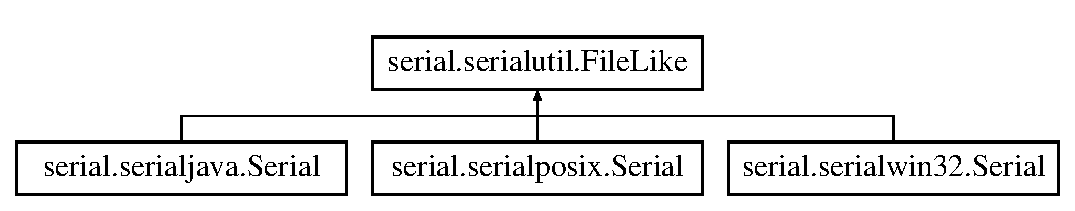
\includegraphics[height=2.000000cm]{classserial_1_1serialutil_1_1_file_like}
\end{center}
\end{figure}
\subsection*{Public Member Functions}
\begin{DoxyCompactItemize}
\item 
\hypertarget{classserial_1_1serialutil_1_1_file_like_a02ccce9ac927311b73130cb084ce3b4f}{def {\bfseries read}}\label{classserial_1_1serialutil_1_1_file_like_a02ccce9ac927311b73130cb084ce3b4f}

\item 
\hypertarget{classserial_1_1serialutil_1_1_file_like_a4ff22b47bd5fdc0fac01b9a409384e5b}{def {\bfseries write}}\label{classserial_1_1serialutil_1_1_file_like_a4ff22b47bd5fdc0fac01b9a409384e5b}

\item 
def \hyperlink{classserial_1_1serialutil_1_1_file_like_a35da6b9eacf5d3b7dd7ee0acd27ea719}{readline}
\item 
def \hyperlink{classserial_1_1serialutil_1_1_file_like_af5ce1f0e6f2b3358cb0b635f89b6dc75}{readlines}
\item 
def \hyperlink{classserial_1_1serialutil_1_1_file_like_a47d04aa3d47054b1fb285d120b0cbbf9}{xreadlines}
\item 
\hypertarget{classserial_1_1serialutil_1_1_file_like_a563678bf0045c4d3efa1787b521c45f5}{def {\bfseries writelines}}\label{classserial_1_1serialutil_1_1_file_like_a563678bf0045c4d3efa1787b521c45f5}

\item 
def \hyperlink{classserial_1_1serialutil_1_1_file_like_ad928665200ce30593f7a86c52e1fb061}{flush}
\end{DoxyCompactItemize}


\subsection{Detailed Description}
\begin{DoxyVerb}An abstract file like class.

This class implements readline and readlines based on read and
writelines based on write.
This class is used to provide the above functions for to Serial
port objects.

Note that when the serial port was opened with _NO_ timeout that
readline blocks until it sees a newline (or the specified size is
reached) and that readlines would never return and therefore
refuses to work (it raises an exception in this case)!
\end{DoxyVerb}
 

\subsection{Member Function Documentation}
\hypertarget{classserial_1_1serialutil_1_1_file_like_ad928665200ce30593f7a86c52e1fb061}{\index{serial\-::serialutil\-::\-File\-Like@{serial\-::serialutil\-::\-File\-Like}!flush@{flush}}
\index{flush@{flush}!serial::serialutil::FileLike@{serial\-::serialutil\-::\-File\-Like}}
\subsubsection[{flush}]{\setlength{\rightskip}{0pt plus 5cm}def serial.\-serialutil.\-File\-Like.\-flush (
\begin{DoxyParamCaption}
\item[{}]{self}
\end{DoxyParamCaption}
)}}\label{classserial_1_1serialutil_1_1_file_like_ad928665200ce30593f7a86c52e1fb061}
\begin{DoxyVerb}flush of file like objects\end{DoxyVerb}
 \hypertarget{classserial_1_1serialutil_1_1_file_like_a35da6b9eacf5d3b7dd7ee0acd27ea719}{\index{serial\-::serialutil\-::\-File\-Like@{serial\-::serialutil\-::\-File\-Like}!readline@{readline}}
\index{readline@{readline}!serial::serialutil::FileLike@{serial\-::serialutil\-::\-File\-Like}}
\subsubsection[{readline}]{\setlength{\rightskip}{0pt plus 5cm}def serial.\-serialutil.\-File\-Like.\-readline (
\begin{DoxyParamCaption}
\item[{}]{self, }
\item[{}]{size = {\ttfamily None}, }
\item[{}]{eol = {\ttfamily '\textbackslash{}n'}}
\end{DoxyParamCaption}
)}}\label{classserial_1_1serialutil_1_1_file_like_a35da6b9eacf5d3b7dd7ee0acd27ea719}
\begin{DoxyVerb}read a line which is terminated with end-of-line (eol) character
('\n' by default) or until timeout\end{DoxyVerb}
 \hypertarget{classserial_1_1serialutil_1_1_file_like_af5ce1f0e6f2b3358cb0b635f89b6dc75}{\index{serial\-::serialutil\-::\-File\-Like@{serial\-::serialutil\-::\-File\-Like}!readlines@{readlines}}
\index{readlines@{readlines}!serial::serialutil::FileLike@{serial\-::serialutil\-::\-File\-Like}}
\subsubsection[{readlines}]{\setlength{\rightskip}{0pt plus 5cm}def serial.\-serialutil.\-File\-Like.\-readlines (
\begin{DoxyParamCaption}
\item[{}]{self, }
\item[{}]{sizehint = {\ttfamily None}, }
\item[{}]{eol = {\ttfamily '\textbackslash{}n'}}
\end{DoxyParamCaption}
)}}\label{classserial_1_1serialutil_1_1_file_like_af5ce1f0e6f2b3358cb0b635f89b6dc75}
\begin{DoxyVerb}read a list of lines, until timeout
sizehint is ignored\end{DoxyVerb}
 \hypertarget{classserial_1_1serialutil_1_1_file_like_a47d04aa3d47054b1fb285d120b0cbbf9}{\index{serial\-::serialutil\-::\-File\-Like@{serial\-::serialutil\-::\-File\-Like}!xreadlines@{xreadlines}}
\index{xreadlines@{xreadlines}!serial::serialutil::FileLike@{serial\-::serialutil\-::\-File\-Like}}
\subsubsection[{xreadlines}]{\setlength{\rightskip}{0pt plus 5cm}def serial.\-serialutil.\-File\-Like.\-xreadlines (
\begin{DoxyParamCaption}
\item[{}]{self, }
\item[{}]{sizehint = {\ttfamily None}}
\end{DoxyParamCaption}
)}}\label{classserial_1_1serialutil_1_1_file_like_a47d04aa3d47054b1fb285d120b0cbbf9}
\begin{DoxyVerb}just call readlines - here for compatibility\end{DoxyVerb}
 

The documentation for this class was generated from the following file\-:\begin{DoxyCompactItemize}
\item 
tools/sky/serial/serialutil.\-py\end{DoxyCompactItemize}

\hypertarget{structprocess}{\section{process Struct Reference}
\label{structprocess}\index{process@{process}}
}
\subsection*{Public Member Functions}
\begin{DoxyCompactItemize}
\item 
\hypertarget{structprocess_a2fc6f517fc51107c3d7a3f82abbd2777}{{\bfseries P\-T\-\_\-\-T\-H\-R\-E\-A\-D} (($\ast$thread)(struct \hyperlink{structpt}{pt} $\ast$, process\-\_\-event\-\_\-t, process\-\_\-data\-\_\-t))}\label{structprocess_a2fc6f517fc51107c3d7a3f82abbd2777}

\end{DoxyCompactItemize}
\subsection*{Public Attributes}
\begin{DoxyCompactItemize}
\item 
\hypertarget{structprocess_aa714b70ab9ca99fc489de2f70a091b0b}{struct \hyperlink{structprocess}{process} $\ast$ {\bfseries next}}\label{structprocess_aa714b70ab9ca99fc489de2f70a091b0b}

\item 
\hypertarget{structprocess_a78b62efdeb69a53c334a2fe0909c84cd}{const char $\ast$ {\bfseries name}}\label{structprocess_a78b62efdeb69a53c334a2fe0909c84cd}

\item 
\hypertarget{structprocess_a68e0ede15bef73b0a641955fe8cb0edd}{struct \hyperlink{structpt}{pt} {\bfseries pt}}\label{structprocess_a68e0ede15bef73b0a641955fe8cb0edd}

\item 
\hypertarget{structprocess_a481a37ac56e19e2a1e65341b0db2b177}{unsigned char {\bfseries state}}\label{structprocess_a481a37ac56e19e2a1e65341b0db2b177}

\item 
\hypertarget{structprocess_a2b2ad213f87d7a470caf9f350a436f7c}{unsigned char {\bfseries needspoll}}\label{structprocess_a2b2ad213f87d7a470caf9f350a436f7c}

\end{DoxyCompactItemize}


The documentation for this struct was generated from the following file\-:\begin{DoxyCompactItemize}
\item 
core/sys/\hyperlink{process_8h}{process.\-h}\end{DoxyCompactItemize}

\hypertarget{structpt}{\section{pt Struct Reference}
\label{structpt}\index{pt@{pt}}
}
\subsection*{Public Attributes}
\begin{DoxyCompactItemize}
\item 
\hypertarget{structpt_ac3fa0fa86689e3e7c039a16c16861dbe}{lc\-\_\-t {\bfseries lc}}\label{structpt_ac3fa0fa86689e3e7c039a16c16861dbe}

\end{DoxyCompactItemize}


The documentation for this struct was generated from the following file\-:\begin{DoxyCompactItemize}
\item 
core/sys/\hyperlink{pt_8h}{pt.\-h}\end{DoxyCompactItemize}

\hypertarget{structpt__sem}{\section{pt\-\_\-sem Struct Reference}
\label{structpt__sem}\index{pt\-\_\-sem@{pt\-\_\-sem}}
}
\subsection*{Public Attributes}
\begin{DoxyCompactItemize}
\item 
\hypertarget{structpt__sem_a6f341120f42d5fd9f329ff1119594743}{unsigned int {\bfseries count}}\label{structpt__sem_a6f341120f42d5fd9f329ff1119594743}

\end{DoxyCompactItemize}


The documentation for this struct was generated from the following file\-:\begin{DoxyCompactItemize}
\item 
core/sys/\hyperlink{pt-sem_8h}{pt-\/sem.\-h}\end{DoxyCompactItemize}

\hypertarget{structringbuf}{\section{ringbuf Struct Reference}
\label{structringbuf}\index{ringbuf@{ringbuf}}
}


Structure that holds the state of a ring buffer.  




{\ttfamily \#include $<$ringbuf.\-h$>$}

\subsection*{Public Attributes}
\begin{DoxyCompactItemize}
\item 
\hypertarget{group__ringbuf_gae1472129ec96ef39782f87836fb670da}{uint8\-\_\-t $\ast$ {\bfseries data}}\label{group__ringbuf_gae1472129ec96ef39782f87836fb670da}

\item 
\hypertarget{group__ringbuf_ga78d6347a4464086fdbae6258c1e603c4}{uint8\-\_\-t {\bfseries mask}}\label{group__ringbuf_ga78d6347a4464086fdbae6258c1e603c4}

\item 
\hypertarget{group__ringbuf_gad8ed0f67d2d85a7707d271ae9386dcf8}{uint8\-\_\-t {\bfseries put\-\_\-ptr}}\label{group__ringbuf_gad8ed0f67d2d85a7707d271ae9386dcf8}

\item 
\hypertarget{group__ringbuf_gaf4b195d1d47a3190deb1d646e9a04528}{uint8\-\_\-t {\bfseries get\-\_\-ptr}}\label{group__ringbuf_gaf4b195d1d47a3190deb1d646e9a04528}

\end{DoxyCompactItemize}


\subsection{Detailed Description}
Structure that holds the state of a ring buffer. 

This structure holds the state of a ring buffer. The actual buffer needs to be defined separately. This struct is an opaque structure with no user-\/visible elements. 

The documentation for this struct was generated from the following file\-:\begin{DoxyCompactItemize}
\item 
core/lib/\hyperlink{ringbuf_8h}{ringbuf.\-h}\end{DoxyCompactItemize}

\hypertarget{structrtimer}{\section{rtimer Struct Reference}
\label{structrtimer}\index{rtimer@{rtimer}}
}


Representation of a real-\/time task.  




{\ttfamily \#include $<$rtimer.\-h$>$}

\subsection*{Public Attributes}
\begin{DoxyCompactItemize}
\item 
\hypertarget{structrtimer_a4a3b4d5f021bfe3026248023e0787423}{rtimer\-\_\-clock\-\_\-t {\bfseries time}}\label{structrtimer_a4a3b4d5f021bfe3026248023e0787423}

\item 
\hypertarget{structrtimer_a8470682ff83caee7e34080545c6a25a6}{rtimer\-\_\-clock\-\_\-t {\bfseries overflows\-\_\-to\-\_\-go}}\label{structrtimer_a8470682ff83caee7e34080545c6a25a6}

\item 
\hypertarget{structrtimer_a7d94e8851e183e8c93e3b7e210eb7212}{rtimer\-\_\-callback\-\_\-t {\bfseries func}}\label{structrtimer_a7d94e8851e183e8c93e3b7e210eb7212}

\item 
\hypertarget{structrtimer_a94cff963392454c4c92ed379b5cf9790}{void $\ast$ {\bfseries ptr}}\label{structrtimer_a94cff963392454c4c92ed379b5cf9790}

\end{DoxyCompactItemize}


\subsection{Detailed Description}
Representation of a real-\/time task. 

This structure represents a real-\/time task and is used by the real-\/time module and the architecture specific support module for the real-\/time module. 

The documentation for this struct was generated from the following file\-:\begin{DoxyCompactItemize}
\item 
core/sys/\hyperlink{rtimer_8h}{rtimer.\-h}\end{DoxyCompactItemize}

\hypertarget{classserial_1_1serialposix_1_1_serial}{\section{serial.\-serialposix.\-Serial Class Reference}
\label{classserial_1_1serialposix_1_1_serial}\index{serial.\-serialposix.\-Serial@{serial.\-serialposix.\-Serial}}
}
Inheritance diagram for serial.\-serialposix.\-Serial\-:\begin{figure}[H]
\begin{center}
\leavevmode
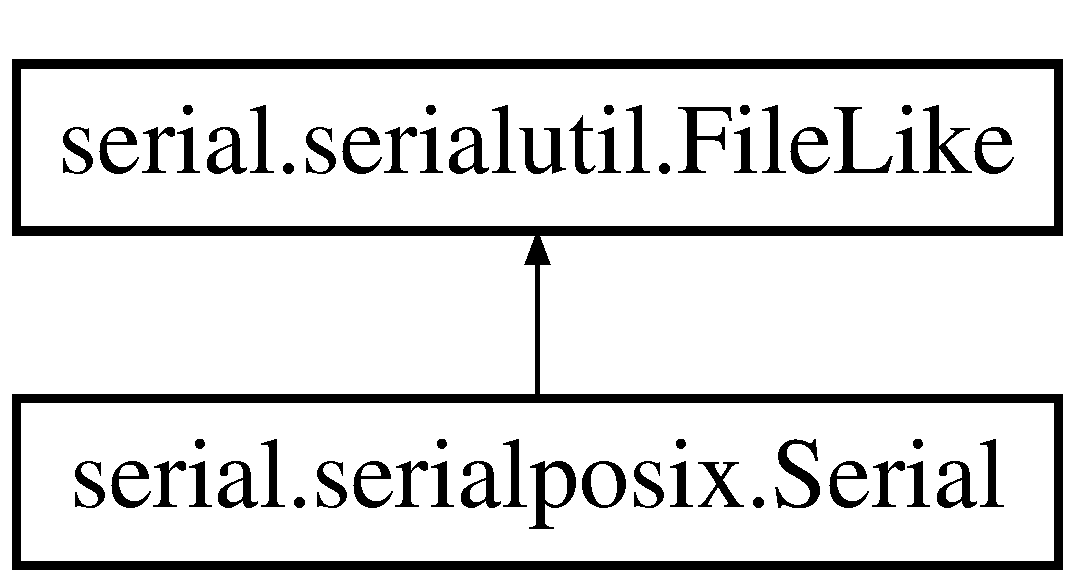
\includegraphics[height=2.000000cm]{classserial_1_1serialposix_1_1_serial}
\end{center}
\end{figure}
\subsection*{Public Member Functions}
\begin{DoxyCompactItemize}
\item 
def \hyperlink{classserial_1_1serialposix_1_1_serial_afbf64348bdf4cbd3b0356e379368950f}{\-\_\-\-\_\-init\-\_\-\-\_\-}
\item 
def \hyperlink{classserial_1_1serialposix_1_1_serial_a160bf0d6861849ee0440bb412bb67ca0}{close}
\item 
def \hyperlink{classserial_1_1serialposix_1_1_serial_ac120a2512d88d1f4453871333f92810e}{set\-Baudrate}
\item 
def \hyperlink{classserial_1_1serialposix_1_1_serial_a281c188a874885c0e51bd50de009b2a4}{in\-Waiting}
\item 
def \hyperlink{classserial_1_1serialposix_1_1_serial_a5f3906413ea14066492e007680c517d8}{write}
\item 
def \hyperlink{classserial_1_1serialposix_1_1_serial_a173d66c3d3cd356d8f90b51f0f750604}{read}
\item 
def \hyperlink{classserial_1_1serialposix_1_1_serial_ae4f788d9e8ae622f69731582aa5fd7dc}{flush\-Input}
\item 
def \hyperlink{classserial_1_1serialposix_1_1_serial_ad77f302127b94b0d1cdf8e8019aae4fc}{flush\-Output}
\item 
def \hyperlink{classserial_1_1serialposix_1_1_serial_a3c7d86701aef4760ce693fc76512065f}{send\-Break}
\item 
def \hyperlink{classserial_1_1serialposix_1_1_serial_a92d20409acba15e0f907a91c91172c16}{drain\-Output}
\item 
def \hyperlink{classserial_1_1serialposix_1_1_serial_a83cbe476662a8ed062eb483ad9c571d0}{nonblocking}
\item 
def \hyperlink{classserial_1_1serialposix_1_1_serial_a33c1bc242b4a5ed5f872fe20e9b95f44}{get\-D\-S\-R}
\item 
def \hyperlink{classserial_1_1serialposix_1_1_serial_afe7450ca115457d4cf8a05e28565b071}{get\-C\-D}
\item 
def \hyperlink{classserial_1_1serialposix_1_1_serial_af2319eee15459a274c33512b5f3e162d}{get\-R\-I}
\item 
def \hyperlink{classserial_1_1serialposix_1_1_serial_ac837d511bbdf6af08ce0fa42789e0dc4}{get\-C\-T\-S}
\item 
def \hyperlink{classserial_1_1serialposix_1_1_serial_a47a43e9a8ef8e589d72b1d65c5ed7c00}{set\-D\-T\-R}
\item 
def \hyperlink{classserial_1_1serialposix_1_1_serial_aa75c59e677d9e641fb371df1a41d5d6f}{set\-R\-T\-S}
\end{DoxyCompactItemize}
\subsection*{Public Attributes}
\begin{DoxyCompactItemize}
\item 
\hypertarget{classserial_1_1serialposix_1_1_serial_aaaf5c903fd97c0e4b26a3a224c4acdba}{{\bfseries fd}}\label{classserial_1_1serialposix_1_1_serial_aaaf5c903fd97c0e4b26a3a224c4acdba}

\item 
\hypertarget{classserial_1_1serialposix_1_1_serial_aa08e7c9fd4c836a7d33bd5bf1a50dfc5}{{\bfseries timeout}}\label{classserial_1_1serialposix_1_1_serial_aa08e7c9fd4c836a7d33bd5bf1a50dfc5}

\item 
\hypertarget{classserial_1_1serialposix_1_1_serial_a4fa822f75d7ff9f401b0719cfb39a3df}{{\bfseries portstr}}\label{classserial_1_1serialposix_1_1_serial_a4fa822f75d7ff9f401b0719cfb39a3df}

\item 
\hypertarget{classserial_1_1serialposix_1_1_serial_aae15d7b931057e36ebd3172d4a09b728}{{\bfseries cflag}}\label{classserial_1_1serialposix_1_1_serial_aae15d7b931057e36ebd3172d4a09b728}

\item 
\hypertarget{classserial_1_1serialposix_1_1_serial_af782e542442f6e792c24de466ada7220}{{\bfseries lflag}}\label{classserial_1_1serialposix_1_1_serial_af782e542442f6e792c24de466ada7220}

\item 
\hypertarget{classserial_1_1serialposix_1_1_serial_aea060f4346acff44b003f6ffddb9f3e5}{{\bfseries oflag}}\label{classserial_1_1serialposix_1_1_serial_aea060f4346acff44b003f6ffddb9f3e5}

\item 
\hypertarget{classserial_1_1serialposix_1_1_serial_ac238b6aaf4c4b4169b99e3b1969aa710}{{\bfseries iflag}}\label{classserial_1_1serialposix_1_1_serial_ac238b6aaf4c4b4169b99e3b1969aa710}

\item 
\hypertarget{classserial_1_1serialposix_1_1_serial_af1fa3027b5be88371748e984a1dd766d}{{\bfseries ispeed}}\label{classserial_1_1serialposix_1_1_serial_af1fa3027b5be88371748e984a1dd766d}

\item 
\hypertarget{classserial_1_1serialposix_1_1_serial_aa3f8581e533b027cc6f6c638cd67d039}{{\bfseries ospeed}}\label{classserial_1_1serialposix_1_1_serial_aa3f8581e533b027cc6f6c638cd67d039}

\item 
\hypertarget{classserial_1_1serialposix_1_1_serial_acd887a620112faa02ffe52581e62070c}{{\bfseries cc}}\label{classserial_1_1serialposix_1_1_serial_acd887a620112faa02ffe52581e62070c}

\end{DoxyCompactItemize}


\subsection{Constructor \& Destructor Documentation}
\hypertarget{classserial_1_1serialposix_1_1_serial_afbf64348bdf4cbd3b0356e379368950f}{\index{serial\-::serialposix\-::\-Serial@{serial\-::serialposix\-::\-Serial}!\-\_\-\-\_\-init\-\_\-\-\_\-@{\-\_\-\-\_\-init\-\_\-\-\_\-}}
\index{\-\_\-\-\_\-init\-\_\-\-\_\-@{\-\_\-\-\_\-init\-\_\-\-\_\-}!serial::serialposix::Serial@{serial\-::serialposix\-::\-Serial}}
\subsubsection[{\-\_\-\-\_\-init\-\_\-\-\_\-}]{\setlength{\rightskip}{0pt plus 5cm}def serial.\-serialposix.\-Serial.\-\_\-\-\_\-init\-\_\-\-\_\- (
\begin{DoxyParamCaption}
\item[{}]{self, }
\item[{}]{port, }
\item[{}]{baudrate = {\ttfamily 9600}, }
\item[{}]{bytesize = {\ttfamily EIGHTBITS}, }
\item[{}]{parity = {\ttfamily PARITY\-\_\-NONE}, }
\item[{}]{stopbits = {\ttfamily STOPBITS\-\_\-ONE}, }
\item[{}]{timeout = {\ttfamily None}, }
\item[{}]{xonxoff = {\ttfamily 0}, }
\item[{}]{rtscts = {\ttfamily 0}}
\end{DoxyParamCaption}
)}}\label{classserial_1_1serialposix_1_1_serial_afbf64348bdf4cbd3b0356e379368950f}
\begin{DoxyVerb}init comm port\end{DoxyVerb}
 

\subsection{Member Function Documentation}
\hypertarget{classserial_1_1serialposix_1_1_serial_a160bf0d6861849ee0440bb412bb67ca0}{\index{serial\-::serialposix\-::\-Serial@{serial\-::serialposix\-::\-Serial}!close@{close}}
\index{close@{close}!serial::serialposix::Serial@{serial\-::serialposix\-::\-Serial}}
\subsubsection[{close}]{\setlength{\rightskip}{0pt plus 5cm}def serial.\-serialposix.\-Serial.\-close (
\begin{DoxyParamCaption}
\item[{}]{self}
\end{DoxyParamCaption}
)}}\label{classserial_1_1serialposix_1_1_serial_a160bf0d6861849ee0440bb412bb67ca0}
\begin{DoxyVerb}close port\end{DoxyVerb}
 \hypertarget{classserial_1_1serialposix_1_1_serial_a92d20409acba15e0f907a91c91172c16}{\index{serial\-::serialposix\-::\-Serial@{serial\-::serialposix\-::\-Serial}!drain\-Output@{drain\-Output}}
\index{drain\-Output@{drain\-Output}!serial::serialposix::Serial@{serial\-::serialposix\-::\-Serial}}
\subsubsection[{drain\-Output}]{\setlength{\rightskip}{0pt plus 5cm}def serial.\-serialposix.\-Serial.\-drain\-Output (
\begin{DoxyParamCaption}
\item[{}]{self}
\end{DoxyParamCaption}
)}}\label{classserial_1_1serialposix_1_1_serial_a92d20409acba15e0f907a91c91172c16}
\begin{DoxyVerb}internal - not portable!\end{DoxyVerb}
 \hypertarget{classserial_1_1serialposix_1_1_serial_ae4f788d9e8ae622f69731582aa5fd7dc}{\index{serial\-::serialposix\-::\-Serial@{serial\-::serialposix\-::\-Serial}!flush\-Input@{flush\-Input}}
\index{flush\-Input@{flush\-Input}!serial::serialposix::Serial@{serial\-::serialposix\-::\-Serial}}
\subsubsection[{flush\-Input}]{\setlength{\rightskip}{0pt plus 5cm}def serial.\-serialposix.\-Serial.\-flush\-Input (
\begin{DoxyParamCaption}
\item[{}]{self}
\end{DoxyParamCaption}
)}}\label{classserial_1_1serialposix_1_1_serial_ae4f788d9e8ae622f69731582aa5fd7dc}
\begin{DoxyVerb}clear input queue\end{DoxyVerb}
 \hypertarget{classserial_1_1serialposix_1_1_serial_ad77f302127b94b0d1cdf8e8019aae4fc}{\index{serial\-::serialposix\-::\-Serial@{serial\-::serialposix\-::\-Serial}!flush\-Output@{flush\-Output}}
\index{flush\-Output@{flush\-Output}!serial::serialposix::Serial@{serial\-::serialposix\-::\-Serial}}
\subsubsection[{flush\-Output}]{\setlength{\rightskip}{0pt plus 5cm}def serial.\-serialposix.\-Serial.\-flush\-Output (
\begin{DoxyParamCaption}
\item[{}]{self}
\end{DoxyParamCaption}
)}}\label{classserial_1_1serialposix_1_1_serial_ad77f302127b94b0d1cdf8e8019aae4fc}
\begin{DoxyVerb}flush output\end{DoxyVerb}
 \hypertarget{classserial_1_1serialposix_1_1_serial_afe7450ca115457d4cf8a05e28565b071}{\index{serial\-::serialposix\-::\-Serial@{serial\-::serialposix\-::\-Serial}!get\-C\-D@{get\-C\-D}}
\index{get\-C\-D@{get\-C\-D}!serial::serialposix::Serial@{serial\-::serialposix\-::\-Serial}}
\subsubsection[{get\-C\-D}]{\setlength{\rightskip}{0pt plus 5cm}def serial.\-serialposix.\-Serial.\-get\-C\-D (
\begin{DoxyParamCaption}
\item[{}]{self}
\end{DoxyParamCaption}
)}}\label{classserial_1_1serialposix_1_1_serial_afe7450ca115457d4cf8a05e28565b071}
\begin{DoxyVerb}read terminal status line\end{DoxyVerb}
 \hypertarget{classserial_1_1serialposix_1_1_serial_ac837d511bbdf6af08ce0fa42789e0dc4}{\index{serial\-::serialposix\-::\-Serial@{serial\-::serialposix\-::\-Serial}!get\-C\-T\-S@{get\-C\-T\-S}}
\index{get\-C\-T\-S@{get\-C\-T\-S}!serial::serialposix::Serial@{serial\-::serialposix\-::\-Serial}}
\subsubsection[{get\-C\-T\-S}]{\setlength{\rightskip}{0pt plus 5cm}def serial.\-serialposix.\-Serial.\-get\-C\-T\-S (
\begin{DoxyParamCaption}
\item[{}]{self}
\end{DoxyParamCaption}
)}}\label{classserial_1_1serialposix_1_1_serial_ac837d511bbdf6af08ce0fa42789e0dc4}
\begin{DoxyVerb}read terminal status line\end{DoxyVerb}
 \hypertarget{classserial_1_1serialposix_1_1_serial_a33c1bc242b4a5ed5f872fe20e9b95f44}{\index{serial\-::serialposix\-::\-Serial@{serial\-::serialposix\-::\-Serial}!get\-D\-S\-R@{get\-D\-S\-R}}
\index{get\-D\-S\-R@{get\-D\-S\-R}!serial::serialposix::Serial@{serial\-::serialposix\-::\-Serial}}
\subsubsection[{get\-D\-S\-R}]{\setlength{\rightskip}{0pt plus 5cm}def serial.\-serialposix.\-Serial.\-get\-D\-S\-R (
\begin{DoxyParamCaption}
\item[{}]{self}
\end{DoxyParamCaption}
)}}\label{classserial_1_1serialposix_1_1_serial_a33c1bc242b4a5ed5f872fe20e9b95f44}
\begin{DoxyVerb}read terminal status line\end{DoxyVerb}
 \hypertarget{classserial_1_1serialposix_1_1_serial_af2319eee15459a274c33512b5f3e162d}{\index{serial\-::serialposix\-::\-Serial@{serial\-::serialposix\-::\-Serial}!get\-R\-I@{get\-R\-I}}
\index{get\-R\-I@{get\-R\-I}!serial::serialposix::Serial@{serial\-::serialposix\-::\-Serial}}
\subsubsection[{get\-R\-I}]{\setlength{\rightskip}{0pt plus 5cm}def serial.\-serialposix.\-Serial.\-get\-R\-I (
\begin{DoxyParamCaption}
\item[{}]{self}
\end{DoxyParamCaption}
)}}\label{classserial_1_1serialposix_1_1_serial_af2319eee15459a274c33512b5f3e162d}
\begin{DoxyVerb}read terminal status line\end{DoxyVerb}
 \hypertarget{classserial_1_1serialposix_1_1_serial_a281c188a874885c0e51bd50de009b2a4}{\index{serial\-::serialposix\-::\-Serial@{serial\-::serialposix\-::\-Serial}!in\-Waiting@{in\-Waiting}}
\index{in\-Waiting@{in\-Waiting}!serial::serialposix::Serial@{serial\-::serialposix\-::\-Serial}}
\subsubsection[{in\-Waiting}]{\setlength{\rightskip}{0pt plus 5cm}def serial.\-serialposix.\-Serial.\-in\-Waiting (
\begin{DoxyParamCaption}
\item[{}]{self}
\end{DoxyParamCaption}
)}}\label{classserial_1_1serialposix_1_1_serial_a281c188a874885c0e51bd50de009b2a4}
\begin{DoxyVerb}how many character are in the input queue\end{DoxyVerb}
 \hypertarget{classserial_1_1serialposix_1_1_serial_a83cbe476662a8ed062eb483ad9c571d0}{\index{serial\-::serialposix\-::\-Serial@{serial\-::serialposix\-::\-Serial}!nonblocking@{nonblocking}}
\index{nonblocking@{nonblocking}!serial::serialposix::Serial@{serial\-::serialposix\-::\-Serial}}
\subsubsection[{nonblocking}]{\setlength{\rightskip}{0pt plus 5cm}def serial.\-serialposix.\-Serial.\-nonblocking (
\begin{DoxyParamCaption}
\item[{}]{self}
\end{DoxyParamCaption}
)}}\label{classserial_1_1serialposix_1_1_serial_a83cbe476662a8ed062eb483ad9c571d0}
\begin{DoxyVerb}internal - not portable!\end{DoxyVerb}
 \hypertarget{classserial_1_1serialposix_1_1_serial_a173d66c3d3cd356d8f90b51f0f750604}{\index{serial\-::serialposix\-::\-Serial@{serial\-::serialposix\-::\-Serial}!read@{read}}
\index{read@{read}!serial::serialposix::Serial@{serial\-::serialposix\-::\-Serial}}
\subsubsection[{read}]{\setlength{\rightskip}{0pt plus 5cm}def serial.\-serialposix.\-Serial.\-read (
\begin{DoxyParamCaption}
\item[{}]{self, }
\item[{}]{size = {\ttfamily 1}}
\end{DoxyParamCaption}
)}}\label{classserial_1_1serialposix_1_1_serial_a173d66c3d3cd356d8f90b51f0f750604}
\begin{DoxyVerb}read a number of bytes from the port.
the default is one (unlike files)\end{DoxyVerb}
 \hypertarget{classserial_1_1serialposix_1_1_serial_a3c7d86701aef4760ce693fc76512065f}{\index{serial\-::serialposix\-::\-Serial@{serial\-::serialposix\-::\-Serial}!send\-Break@{send\-Break}}
\index{send\-Break@{send\-Break}!serial::serialposix::Serial@{serial\-::serialposix\-::\-Serial}}
\subsubsection[{send\-Break}]{\setlength{\rightskip}{0pt plus 5cm}def serial.\-serialposix.\-Serial.\-send\-Break (
\begin{DoxyParamCaption}
\item[{}]{self}
\end{DoxyParamCaption}
)}}\label{classserial_1_1serialposix_1_1_serial_a3c7d86701aef4760ce693fc76512065f}
\begin{DoxyVerb}send break signal\end{DoxyVerb}
 \hypertarget{classserial_1_1serialposix_1_1_serial_ac120a2512d88d1f4453871333f92810e}{\index{serial\-::serialposix\-::\-Serial@{serial\-::serialposix\-::\-Serial}!set\-Baudrate@{set\-Baudrate}}
\index{set\-Baudrate@{set\-Baudrate}!serial::serialposix::Serial@{serial\-::serialposix\-::\-Serial}}
\subsubsection[{set\-Baudrate}]{\setlength{\rightskip}{0pt plus 5cm}def serial.\-serialposix.\-Serial.\-set\-Baudrate (
\begin{DoxyParamCaption}
\item[{}]{self, }
\item[{}]{baudrate}
\end{DoxyParamCaption}
)}}\label{classserial_1_1serialposix_1_1_serial_ac120a2512d88d1f4453871333f92810e}
\begin{DoxyVerb}change baudrate after port is open\end{DoxyVerb}
 \hypertarget{classserial_1_1serialposix_1_1_serial_a47a43e9a8ef8e589d72b1d65c5ed7c00}{\index{serial\-::serialposix\-::\-Serial@{serial\-::serialposix\-::\-Serial}!set\-D\-T\-R@{set\-D\-T\-R}}
\index{set\-D\-T\-R@{set\-D\-T\-R}!serial::serialposix::Serial@{serial\-::serialposix\-::\-Serial}}
\subsubsection[{set\-D\-T\-R}]{\setlength{\rightskip}{0pt plus 5cm}def serial.\-serialposix.\-Serial.\-set\-D\-T\-R (
\begin{DoxyParamCaption}
\item[{}]{self, }
\item[{}]{on = {\ttfamily 1}}
\end{DoxyParamCaption}
)}}\label{classserial_1_1serialposix_1_1_serial_a47a43e9a8ef8e589d72b1d65c5ed7c00}
\begin{DoxyVerb}set terminal status line\end{DoxyVerb}
 \hypertarget{classserial_1_1serialposix_1_1_serial_aa75c59e677d9e641fb371df1a41d5d6f}{\index{serial\-::serialposix\-::\-Serial@{serial\-::serialposix\-::\-Serial}!set\-R\-T\-S@{set\-R\-T\-S}}
\index{set\-R\-T\-S@{set\-R\-T\-S}!serial::serialposix::Serial@{serial\-::serialposix\-::\-Serial}}
\subsubsection[{set\-R\-T\-S}]{\setlength{\rightskip}{0pt plus 5cm}def serial.\-serialposix.\-Serial.\-set\-R\-T\-S (
\begin{DoxyParamCaption}
\item[{}]{self, }
\item[{}]{on = {\ttfamily 1}}
\end{DoxyParamCaption}
)}}\label{classserial_1_1serialposix_1_1_serial_aa75c59e677d9e641fb371df1a41d5d6f}
\begin{DoxyVerb}set terminal status line\end{DoxyVerb}
 \hypertarget{classserial_1_1serialposix_1_1_serial_a5f3906413ea14066492e007680c517d8}{\index{serial\-::serialposix\-::\-Serial@{serial\-::serialposix\-::\-Serial}!write@{write}}
\index{write@{write}!serial::serialposix::Serial@{serial\-::serialposix\-::\-Serial}}
\subsubsection[{write}]{\setlength{\rightskip}{0pt plus 5cm}def serial.\-serialposix.\-Serial.\-write (
\begin{DoxyParamCaption}
\item[{}]{self, }
\item[{}]{data}
\end{DoxyParamCaption}
)}}\label{classserial_1_1serialposix_1_1_serial_a5f3906413ea14066492e007680c517d8}
\begin{DoxyVerb}write a string to the port\end{DoxyVerb}
 

The documentation for this class was generated from the following file\-:\begin{DoxyCompactItemize}
\item 
tools/sky/serial/serialposix.\-py\end{DoxyCompactItemize}

\hypertarget{classserial_1_1serialwin32_1_1_serial}{\section{serial.\-serialwin32.\-Serial Class Reference}
\label{classserial_1_1serialwin32_1_1_serial}\index{serial.\-serialwin32.\-Serial@{serial.\-serialwin32.\-Serial}}
}
Inheritance diagram for serial.\-serialwin32.\-Serial\-:\begin{figure}[H]
\begin{center}
\leavevmode
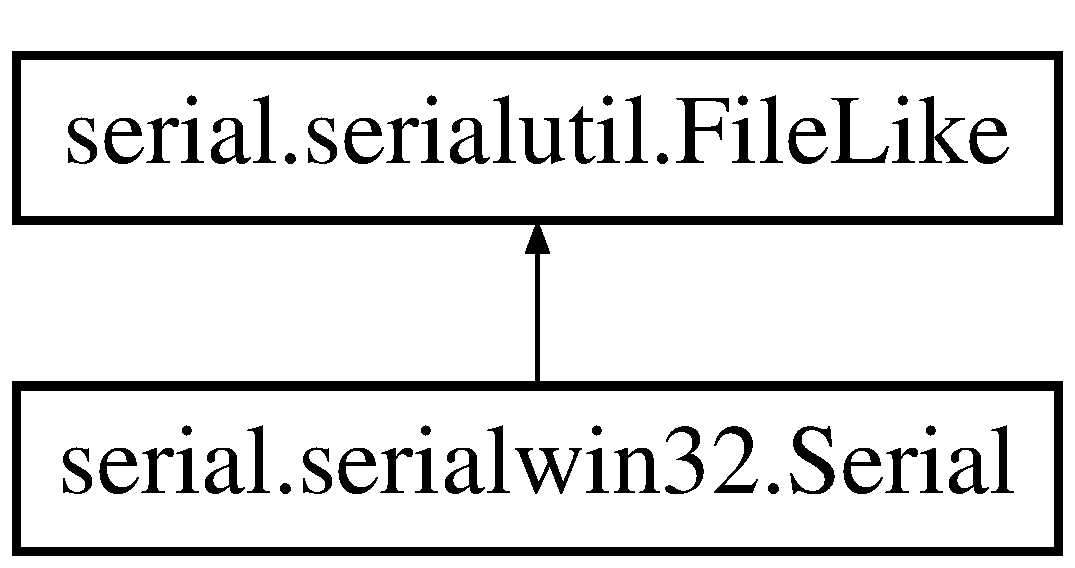
\includegraphics[height=2.000000cm]{classserial_1_1serialwin32_1_1_serial}
\end{center}
\end{figure}
\subsection*{Public Member Functions}
\begin{DoxyCompactItemize}
\item 
def \hyperlink{classserial_1_1serialwin32_1_1_serial_a496d79e84b2e54cb421e29fe0aded074}{\-\_\-\-\_\-init\-\_\-\-\_\-}
\item 
\hypertarget{classserial_1_1serialwin32_1_1_serial_a3a261255c5077d9d36fc7f01321117fe}{def {\bfseries \-\_\-\-\_\-del\-\_\-\-\_\-}}\label{classserial_1_1serialwin32_1_1_serial_a3a261255c5077d9d36fc7f01321117fe}

\item 
def \hyperlink{classserial_1_1serialwin32_1_1_serial_a84c8d26d8bc4c900279841a439a36e9a}{close}
\item 
def \hyperlink{classserial_1_1serialwin32_1_1_serial_a27ba1ff7129d10686e81e6091f9f3cca}{set\-Baudrate}
\item 
def \hyperlink{classserial_1_1serialwin32_1_1_serial_a218b909b445cf9e68aaf5e58c649dd77}{in\-Waiting}
\item 
\hypertarget{classserial_1_1serialwin32_1_1_serial_ac4a825bf4ca093c2dd3f9cb492b1f8b6}{def {\bfseries read}}\label{classserial_1_1serialwin32_1_1_serial_ac4a825bf4ca093c2dd3f9cb492b1f8b6}

\item 
\hypertarget{classserial_1_1serialwin32_1_1_serial_acc20ff5a06c1a7d719c65146068a0526}{def {\bfseries write}}\label{classserial_1_1serialwin32_1_1_serial_acc20ff5a06c1a7d719c65146068a0526}

\item 
\hypertarget{classserial_1_1serialwin32_1_1_serial_a99d1d815de2b6f078e0d010992ee3b10}{def {\bfseries flush\-Input}}\label{classserial_1_1serialwin32_1_1_serial_a99d1d815de2b6f078e0d010992ee3b10}

\item 
\hypertarget{classserial_1_1serialwin32_1_1_serial_a78c782edbc022d76370490f7b2d94508}{def {\bfseries flush\-Output}}\label{classserial_1_1serialwin32_1_1_serial_a78c782edbc022d76370490f7b2d94508}

\item 
\hypertarget{classserial_1_1serialwin32_1_1_serial_a8bc06dd407e906f96685c341830993c7}{def {\bfseries send\-Break}}\label{classserial_1_1serialwin32_1_1_serial_a8bc06dd407e906f96685c341830993c7}

\item 
def \hyperlink{classserial_1_1serialwin32_1_1_serial_afb3008aadbf604ff7cc5fa373fb424c2}{set\-R\-T\-S}
\item 
def \hyperlink{classserial_1_1serialwin32_1_1_serial_aa9d340907457356c3ebe533836213e5a}{set\-D\-T\-R}
\item 
def \hyperlink{classserial_1_1serialwin32_1_1_serial_a9be846f1730355c405c64891790d2a7d}{get\-C\-T\-S}
\item 
def \hyperlink{classserial_1_1serialwin32_1_1_serial_a80e2aa9e9d84a3d4b0dd2d98eac2b92c}{get\-D\-S\-R}
\item 
def \hyperlink{classserial_1_1serialwin32_1_1_serial_ac8e1037e285915f7e2c897fb2a6bfcfd}{get\-R\-I}
\item 
def \hyperlink{classserial_1_1serialwin32_1_1_serial_aa40a3bc1db64a222bfca3f60cfc66b85}{get\-C\-D}
\end{DoxyCompactItemize}
\subsection*{Public Attributes}
\begin{DoxyCompactItemize}
\item 
\hypertarget{classserial_1_1serialwin32_1_1_serial_ae703b88bd0d51ad74f5a26930a87c4ae}{{\bfseries timeout}}\label{classserial_1_1serialwin32_1_1_serial_ae703b88bd0d51ad74f5a26930a87c4ae}

\item 
\hypertarget{classserial_1_1serialwin32_1_1_serial_ac8af1a65407a925ad3a0f8e1a704e054}{{\bfseries portstr}}\label{classserial_1_1serialwin32_1_1_serial_ac8af1a65407a925ad3a0f8e1a704e054}

\item 
\hypertarget{classserial_1_1serialwin32_1_1_serial_a7c4227fd3873cc50afc7685e0f8dfbee}{{\bfseries h\-Com\-Port}}\label{classserial_1_1serialwin32_1_1_serial_a7c4227fd3873cc50afc7685e0f8dfbee}

\item 
\hypertarget{classserial_1_1serialwin32_1_1_serial_ad83b96a33d9ff14a24564e3edd6a13d5}{{\bfseries org\-Timeouts}}\label{classserial_1_1serialwin32_1_1_serial_ad83b96a33d9ff14a24564e3edd6a13d5}

\end{DoxyCompactItemize}


\subsection{Constructor \& Destructor Documentation}
\hypertarget{classserial_1_1serialwin32_1_1_serial_a496d79e84b2e54cb421e29fe0aded074}{\index{serial\-::serialwin32\-::\-Serial@{serial\-::serialwin32\-::\-Serial}!\-\_\-\-\_\-init\-\_\-\-\_\-@{\-\_\-\-\_\-init\-\_\-\-\_\-}}
\index{\-\_\-\-\_\-init\-\_\-\-\_\-@{\-\_\-\-\_\-init\-\_\-\-\_\-}!serial::serialwin32::Serial@{serial\-::serialwin32\-::\-Serial}}
\subsubsection[{\-\_\-\-\_\-init\-\_\-\-\_\-}]{\setlength{\rightskip}{0pt plus 5cm}def serial.\-serialwin32.\-Serial.\-\_\-\-\_\-init\-\_\-\-\_\- (
\begin{DoxyParamCaption}
\item[{}]{self, }
\item[{}]{port, }
\item[{}]{baudrate = {\ttfamily 9600}, }
\item[{}]{bytesize = {\ttfamily EIGHTBITS}, }
\item[{}]{parity = {\ttfamily PARITY\-\_\-NONE}, }
\item[{}]{stopbits = {\ttfamily STOPBITS\-\_\-ONE}, }
\item[{}]{timeout = {\ttfamily None}, }
\item[{}]{xonxoff = {\ttfamily 0}, }
\item[{}]{rtscts = {\ttfamily 0}}
\end{DoxyParamCaption}
)}}\label{classserial_1_1serialwin32_1_1_serial_a496d79e84b2e54cb421e29fe0aded074}
\begin{DoxyVerb}initialize comm port\end{DoxyVerb}
 

\subsection{Member Function Documentation}
\hypertarget{classserial_1_1serialwin32_1_1_serial_a84c8d26d8bc4c900279841a439a36e9a}{\index{serial\-::serialwin32\-::\-Serial@{serial\-::serialwin32\-::\-Serial}!close@{close}}
\index{close@{close}!serial::serialwin32::Serial@{serial\-::serialwin32\-::\-Serial}}
\subsubsection[{close}]{\setlength{\rightskip}{0pt plus 5cm}def serial.\-serialwin32.\-Serial.\-close (
\begin{DoxyParamCaption}
\item[{}]{self}
\end{DoxyParamCaption}
)}}\label{classserial_1_1serialwin32_1_1_serial_a84c8d26d8bc4c900279841a439a36e9a}
\begin{DoxyVerb}close port\end{DoxyVerb}
 \hypertarget{classserial_1_1serialwin32_1_1_serial_aa40a3bc1db64a222bfca3f60cfc66b85}{\index{serial\-::serialwin32\-::\-Serial@{serial\-::serialwin32\-::\-Serial}!get\-C\-D@{get\-C\-D}}
\index{get\-C\-D@{get\-C\-D}!serial::serialwin32::Serial@{serial\-::serialwin32\-::\-Serial}}
\subsubsection[{get\-C\-D}]{\setlength{\rightskip}{0pt plus 5cm}def serial.\-serialwin32.\-Serial.\-get\-C\-D (
\begin{DoxyParamCaption}
\item[{}]{self}
\end{DoxyParamCaption}
)}}\label{classserial_1_1serialwin32_1_1_serial_aa40a3bc1db64a222bfca3f60cfc66b85}
\begin{DoxyVerb}read terminal status line\end{DoxyVerb}
 \hypertarget{classserial_1_1serialwin32_1_1_serial_a9be846f1730355c405c64891790d2a7d}{\index{serial\-::serialwin32\-::\-Serial@{serial\-::serialwin32\-::\-Serial}!get\-C\-T\-S@{get\-C\-T\-S}}
\index{get\-C\-T\-S@{get\-C\-T\-S}!serial::serialwin32::Serial@{serial\-::serialwin32\-::\-Serial}}
\subsubsection[{get\-C\-T\-S}]{\setlength{\rightskip}{0pt plus 5cm}def serial.\-serialwin32.\-Serial.\-get\-C\-T\-S (
\begin{DoxyParamCaption}
\item[{}]{self}
\end{DoxyParamCaption}
)}}\label{classserial_1_1serialwin32_1_1_serial_a9be846f1730355c405c64891790d2a7d}
\begin{DoxyVerb}read terminal status line\end{DoxyVerb}
 \hypertarget{classserial_1_1serialwin32_1_1_serial_a80e2aa9e9d84a3d4b0dd2d98eac2b92c}{\index{serial\-::serialwin32\-::\-Serial@{serial\-::serialwin32\-::\-Serial}!get\-D\-S\-R@{get\-D\-S\-R}}
\index{get\-D\-S\-R@{get\-D\-S\-R}!serial::serialwin32::Serial@{serial\-::serialwin32\-::\-Serial}}
\subsubsection[{get\-D\-S\-R}]{\setlength{\rightskip}{0pt plus 5cm}def serial.\-serialwin32.\-Serial.\-get\-D\-S\-R (
\begin{DoxyParamCaption}
\item[{}]{self}
\end{DoxyParamCaption}
)}}\label{classserial_1_1serialwin32_1_1_serial_a80e2aa9e9d84a3d4b0dd2d98eac2b92c}
\begin{DoxyVerb}read terminal status line\end{DoxyVerb}
 \hypertarget{classserial_1_1serialwin32_1_1_serial_ac8e1037e285915f7e2c897fb2a6bfcfd}{\index{serial\-::serialwin32\-::\-Serial@{serial\-::serialwin32\-::\-Serial}!get\-R\-I@{get\-R\-I}}
\index{get\-R\-I@{get\-R\-I}!serial::serialwin32::Serial@{serial\-::serialwin32\-::\-Serial}}
\subsubsection[{get\-R\-I}]{\setlength{\rightskip}{0pt plus 5cm}def serial.\-serialwin32.\-Serial.\-get\-R\-I (
\begin{DoxyParamCaption}
\item[{}]{self}
\end{DoxyParamCaption}
)}}\label{classserial_1_1serialwin32_1_1_serial_ac8e1037e285915f7e2c897fb2a6bfcfd}
\begin{DoxyVerb}read terminal status line\end{DoxyVerb}
 \hypertarget{classserial_1_1serialwin32_1_1_serial_a218b909b445cf9e68aaf5e58c649dd77}{\index{serial\-::serialwin32\-::\-Serial@{serial\-::serialwin32\-::\-Serial}!in\-Waiting@{in\-Waiting}}
\index{in\-Waiting@{in\-Waiting}!serial::serialwin32::Serial@{serial\-::serialwin32\-::\-Serial}}
\subsubsection[{in\-Waiting}]{\setlength{\rightskip}{0pt plus 5cm}def serial.\-serialwin32.\-Serial.\-in\-Waiting (
\begin{DoxyParamCaption}
\item[{}]{self}
\end{DoxyParamCaption}
)}}\label{classserial_1_1serialwin32_1_1_serial_a218b909b445cf9e68aaf5e58c649dd77}
\begin{DoxyVerb}returns the number of bytes waiting to be read\end{DoxyVerb}
 \hypertarget{classserial_1_1serialwin32_1_1_serial_a27ba1ff7129d10686e81e6091f9f3cca}{\index{serial\-::serialwin32\-::\-Serial@{serial\-::serialwin32\-::\-Serial}!set\-Baudrate@{set\-Baudrate}}
\index{set\-Baudrate@{set\-Baudrate}!serial::serialwin32::Serial@{serial\-::serialwin32\-::\-Serial}}
\subsubsection[{set\-Baudrate}]{\setlength{\rightskip}{0pt plus 5cm}def serial.\-serialwin32.\-Serial.\-set\-Baudrate (
\begin{DoxyParamCaption}
\item[{}]{self, }
\item[{}]{baudrate}
\end{DoxyParamCaption}
)}}\label{classserial_1_1serialwin32_1_1_serial_a27ba1ff7129d10686e81e6091f9f3cca}
\begin{DoxyVerb}change baudrate after port is open\end{DoxyVerb}
 \hypertarget{classserial_1_1serialwin32_1_1_serial_aa9d340907457356c3ebe533836213e5a}{\index{serial\-::serialwin32\-::\-Serial@{serial\-::serialwin32\-::\-Serial}!set\-D\-T\-R@{set\-D\-T\-R}}
\index{set\-D\-T\-R@{set\-D\-T\-R}!serial::serialwin32::Serial@{serial\-::serialwin32\-::\-Serial}}
\subsubsection[{set\-D\-T\-R}]{\setlength{\rightskip}{0pt plus 5cm}def serial.\-serialwin32.\-Serial.\-set\-D\-T\-R (
\begin{DoxyParamCaption}
\item[{}]{self, }
\item[{}]{level = {\ttfamily 1}}
\end{DoxyParamCaption}
)}}\label{classserial_1_1serialwin32_1_1_serial_aa9d340907457356c3ebe533836213e5a}
\begin{DoxyVerb}set terminal status line\end{DoxyVerb}
 \hypertarget{classserial_1_1serialwin32_1_1_serial_afb3008aadbf604ff7cc5fa373fb424c2}{\index{serial\-::serialwin32\-::\-Serial@{serial\-::serialwin32\-::\-Serial}!set\-R\-T\-S@{set\-R\-T\-S}}
\index{set\-R\-T\-S@{set\-R\-T\-S}!serial::serialwin32::Serial@{serial\-::serialwin32\-::\-Serial}}
\subsubsection[{set\-R\-T\-S}]{\setlength{\rightskip}{0pt plus 5cm}def serial.\-serialwin32.\-Serial.\-set\-R\-T\-S (
\begin{DoxyParamCaption}
\item[{}]{self, }
\item[{}]{level = {\ttfamily 1}}
\end{DoxyParamCaption}
)}}\label{classserial_1_1serialwin32_1_1_serial_afb3008aadbf604ff7cc5fa373fb424c2}
\begin{DoxyVerb}set terminal status line\end{DoxyVerb}
 

The documentation for this class was generated from the following file\-:\begin{DoxyCompactItemize}
\item 
tools/sky/serial/serialwin32.\-py\end{DoxyCompactItemize}

\hypertarget{classserial_1_1serialjava_1_1_serial}{\section{serial.\-serialjava.\-Serial Class Reference}
\label{classserial_1_1serialjava_1_1_serial}\index{serial.\-serialjava.\-Serial@{serial.\-serialjava.\-Serial}}
}
Inheritance diagram for serial.\-serialjava.\-Serial\-:\begin{figure}[H]
\begin{center}
\leavevmode
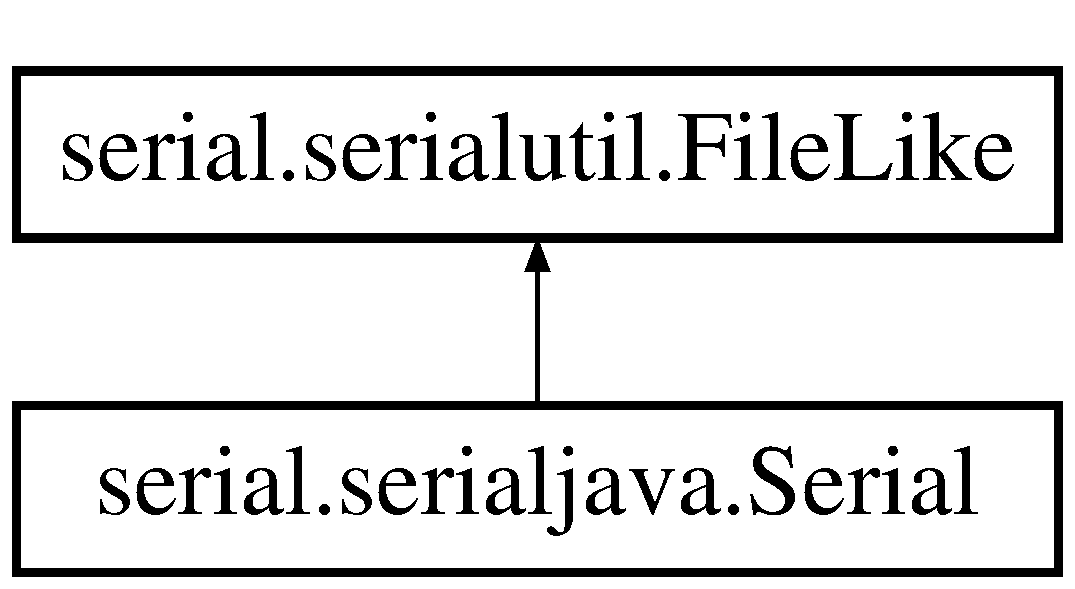
\includegraphics[height=2.000000cm]{classserial_1_1serialjava_1_1_serial}
\end{center}
\end{figure}
\subsection*{Public Member Functions}
\begin{DoxyCompactItemize}
\item 
\hypertarget{classserial_1_1serialjava_1_1_serial_ac4dfc29fc258e1d5e9ceefde89c74bd5}{def {\bfseries \-\_\-\-\_\-init\-\_\-\-\_\-}}\label{classserial_1_1serialjava_1_1_serial_ac4dfc29fc258e1d5e9ceefde89c74bd5}

\item 
\hypertarget{classserial_1_1serialjava_1_1_serial_ac7e556413ed75760aa94e3cca1527a20}{def {\bfseries close}}\label{classserial_1_1serialjava_1_1_serial_ac7e556413ed75760aa94e3cca1527a20}

\item 
def \hyperlink{classserial_1_1serialjava_1_1_serial_a84bb91d0f817d6836a8663c816d16c20}{set\-Baudrate}
\item 
\hypertarget{classserial_1_1serialjava_1_1_serial_abab9fdcfd72dab8510f2f23acdeab604}{def {\bfseries in\-Waiting}}\label{classserial_1_1serialjava_1_1_serial_abab9fdcfd72dab8510f2f23acdeab604}

\item 
\hypertarget{classserial_1_1serialjava_1_1_serial_ac449aeafdaa62aeda707ed5560d36b29}{def {\bfseries write}}\label{classserial_1_1serialjava_1_1_serial_ac449aeafdaa62aeda707ed5560d36b29}

\item 
\hypertarget{classserial_1_1serialjava_1_1_serial_ae71c04f73bab6ee003a8715d82766990}{def {\bfseries read}}\label{classserial_1_1serialjava_1_1_serial_ae71c04f73bab6ee003a8715d82766990}

\item 
\hypertarget{classserial_1_1serialjava_1_1_serial_a8dc207e20ff59b4805fc1f81276a8a29}{def {\bfseries flush\-Input}}\label{classserial_1_1serialjava_1_1_serial_a8dc207e20ff59b4805fc1f81276a8a29}

\item 
\hypertarget{classserial_1_1serialjava_1_1_serial_a53d55c5e44953db4219d1eea4535aa81}{def {\bfseries flush\-Output}}\label{classserial_1_1serialjava_1_1_serial_a53d55c5e44953db4219d1eea4535aa81}

\item 
\hypertarget{classserial_1_1serialjava_1_1_serial_ab5e0414b7092ed2f23898de8b3c49a09}{def {\bfseries send\-Break}}\label{classserial_1_1serialjava_1_1_serial_ab5e0414b7092ed2f23898de8b3c49a09}

\item 
\hypertarget{classserial_1_1serialjava_1_1_serial_ab884f9d59c4c430e403fb95a44cd1281}{def {\bfseries get\-D\-S\-R}}\label{classserial_1_1serialjava_1_1_serial_ab884f9d59c4c430e403fb95a44cd1281}

\item 
\hypertarget{classserial_1_1serialjava_1_1_serial_a87b5b9084944dfdfeb9b421c9d885a87}{def {\bfseries get\-C\-D}}\label{classserial_1_1serialjava_1_1_serial_a87b5b9084944dfdfeb9b421c9d885a87}

\item 
\hypertarget{classserial_1_1serialjava_1_1_serial_a764948606ad2568b8664938ad5ffb0ea}{def {\bfseries get\-R\-I}}\label{classserial_1_1serialjava_1_1_serial_a764948606ad2568b8664938ad5ffb0ea}

\item 
\hypertarget{classserial_1_1serialjava_1_1_serial_ab483902106a2b995dcb785dd309aa9d3}{def {\bfseries get\-C\-T\-S}}\label{classserial_1_1serialjava_1_1_serial_ab483902106a2b995dcb785dd309aa9d3}

\item 
\hypertarget{classserial_1_1serialjava_1_1_serial_a561e55483f92a401e89856c0528a414f}{def {\bfseries set\-D\-T\-R}}\label{classserial_1_1serialjava_1_1_serial_a561e55483f92a401e89856c0528a414f}

\item 
\hypertarget{classserial_1_1serialjava_1_1_serial_a687439a4fa34dc2e0fbde0fbbeb5e813}{def {\bfseries set\-R\-T\-S}}\label{classserial_1_1serialjava_1_1_serial_a687439a4fa34dc2e0fbde0fbbeb5e813}

\end{DoxyCompactItemize}
\subsection*{Public Attributes}
\begin{DoxyCompactItemize}
\item 
\hypertarget{classserial_1_1serialjava_1_1_serial_ab6498afad653a048b71bf6acfa28b9fa}{{\bfseries portstr}}\label{classserial_1_1serialjava_1_1_serial_ab6498afad653a048b71bf6acfa28b9fa}

\item 
\hypertarget{classserial_1_1serialjava_1_1_serial_aaa1990322f62a49afb17fa9dbc0768f2}{{\bfseries s\-Port}}\label{classserial_1_1serialjava_1_1_serial_aaa1990322f62a49afb17fa9dbc0768f2}

\item 
\hypertarget{classserial_1_1serialjava_1_1_serial_a8f441d3c724801dd6d96159e49736aec}{{\bfseries instream}}\label{classserial_1_1serialjava_1_1_serial_a8f441d3c724801dd6d96159e49736aec}

\item 
\hypertarget{classserial_1_1serialjava_1_1_serial_ae3abd44d3b3cdc04e372272c37a9f835}{{\bfseries outstream}}\label{classserial_1_1serialjava_1_1_serial_ae3abd44d3b3cdc04e372272c37a9f835}

\item 
\hypertarget{classserial_1_1serialjava_1_1_serial_abaa47aca86acd764c31bad2b06da90dd}{{\bfseries databits}}\label{classserial_1_1serialjava_1_1_serial_abaa47aca86acd764c31bad2b06da90dd}

\item 
\hypertarget{classserial_1_1serialjava_1_1_serial_ae48fd405b11937ade2efddcfa610c6fb}{{\bfseries jstopbits}}\label{classserial_1_1serialjava_1_1_serial_ae48fd405b11937ade2efddcfa610c6fb}

\item 
\hypertarget{classserial_1_1serialjava_1_1_serial_a198c5f67ae8aaad770a73c4646527225}{{\bfseries jparity}}\label{classserial_1_1serialjava_1_1_serial_a198c5f67ae8aaad770a73c4646527225}

\item 
\hypertarget{classserial_1_1serialjava_1_1_serial_a41c3f66d51a2ea75cb784ed93d23db46}{{\bfseries timeout}}\label{classserial_1_1serialjava_1_1_serial_a41c3f66d51a2ea75cb784ed93d23db46}

\end{DoxyCompactItemize}


\subsection{Member Function Documentation}
\hypertarget{classserial_1_1serialjava_1_1_serial_a84bb91d0f817d6836a8663c816d16c20}{\index{serial\-::serialjava\-::\-Serial@{serial\-::serialjava\-::\-Serial}!set\-Baudrate@{set\-Baudrate}}
\index{set\-Baudrate@{set\-Baudrate}!serial::serialjava::Serial@{serial\-::serialjava\-::\-Serial}}
\subsubsection[{set\-Baudrate}]{\setlength{\rightskip}{0pt plus 5cm}def serial.\-serialjava.\-Serial.\-set\-Baudrate (
\begin{DoxyParamCaption}
\item[{}]{self, }
\item[{}]{baudrate}
\end{DoxyParamCaption}
)}}\label{classserial_1_1serialjava_1_1_serial_a84bb91d0f817d6836a8663c816d16c20}
\begin{DoxyVerb}change baudrate after port is open\end{DoxyVerb}
 

The documentation for this class was generated from the following file\-:\begin{DoxyCompactItemize}
\item 
tools/sky/serial/serialjava.\-py\end{DoxyCompactItemize}

\hypertarget{classserial_1_1serialutil_1_1_serial_exception}{\section{serial.\-serialutil.\-Serial\-Exception Class Reference}
\label{classserial_1_1serialutil_1_1_serial_exception}\index{serial.\-serialutil.\-Serial\-Exception@{serial.\-serialutil.\-Serial\-Exception}}
}
Inheritance diagram for serial.\-serialutil.\-Serial\-Exception\-:\begin{figure}[H]
\begin{center}
\leavevmode
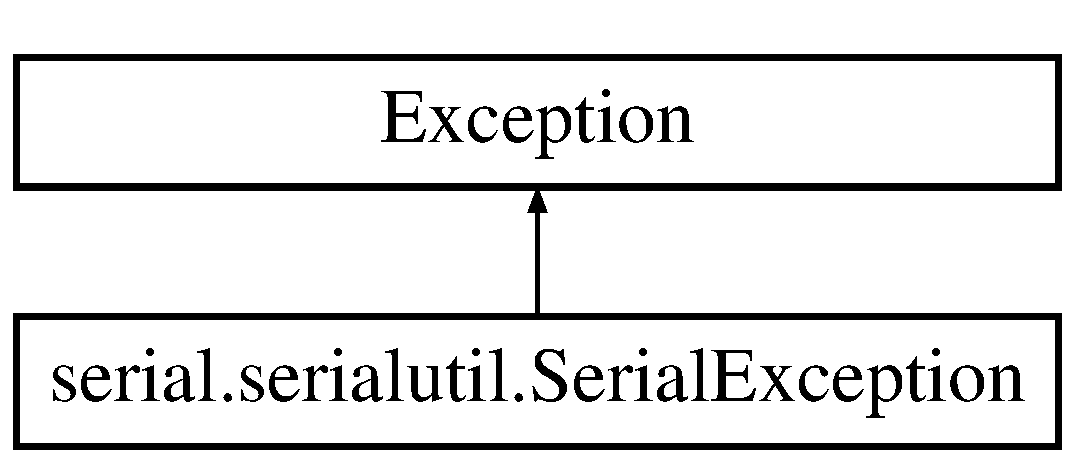
\includegraphics[height=2.000000cm]{classserial_1_1serialutil_1_1_serial_exception}
\end{center}
\end{figure}


The documentation for this class was generated from the following file\-:\begin{DoxyCompactItemize}
\item 
tools/sky/serial/serialutil.\-py\end{DoxyCompactItemize}

\hypertarget{structsymbols}{\section{symbols Struct Reference}
\label{structsymbols}\index{symbols@{symbols}}
}
\subsection*{Public Attributes}
\begin{DoxyCompactItemize}
\item 
\hypertarget{structsymbols_ad73d3966f0a622b936f9eaee6b603bfc}{const char $\ast$ {\bfseries name}}\label{structsymbols_ad73d3966f0a622b936f9eaee6b603bfc}

\item 
\hypertarget{structsymbols_aa7586550f570c0e7e1aa3455a5875a87}{void $\ast$ {\bfseries value}}\label{structsymbols_aa7586550f570c0e7e1aa3455a5875a87}

\end{DoxyCompactItemize}


The documentation for this struct was generated from the following file\-:\begin{DoxyCompactItemize}
\item 
core/loader/symbols.\-h\end{DoxyCompactItemize}

\hypertarget{structtimer}{\section{timer Struct Reference}
\label{structtimer}\index{timer@{timer}}
}


{\ttfamily \#include $<$timer.\-h$>$}

\subsection*{Public Attributes}
\begin{DoxyCompactItemize}
\item 
\hypertarget{structtimer_ae8eb428c05bc1dee022246a3063d277c}{clock\-\_\-time\-\_\-t {\bfseries start}}\label{structtimer_ae8eb428c05bc1dee022246a3063d277c}

\item 
\hypertarget{structtimer_afe557d333c06cf65f52023f45f5b0a3a}{clock\-\_\-time\-\_\-t {\bfseries interval}}\label{structtimer_afe557d333c06cf65f52023f45f5b0a3a}

\end{DoxyCompactItemize}


\subsection{Detailed Description}
A timer.

This structure is used for declaring a timer. The timer must be set with \hyperlink{group__timer_ga6614d96fdfcd95c95ec6e6f63071ff51}{timer\-\_\-set()} before it can be used. 

The documentation for this struct was generated from the following file\-:\begin{DoxyCompactItemize}
\item 
core/sys/\hyperlink{timer_8h}{timer.\-h}\end{DoxyCompactItemize}

\chapter{File Documentation}
\hypertarget{chaos-test_8c}{\section{apps/chaos-\/test/chaos-\/test.c File Reference}
\label{chaos-test_8c}\index{apps/chaos-\/test/chaos-\/test.\-c@{apps/chaos-\/test/chaos-\/test.\-c}}
}
{\ttfamily \#include \char`\"{}chaos-\/test.\-h\char`\"{}}\\*
{\ttfamily \#include \char`\"{}chaos.\-h\char`\"{}}\\*
\subsection*{Functions}
\begin{DoxyCompactItemize}
\item 
\hypertarget{group__chaos-test-print-stats_gaba1b7c42a3ed004b9bd807614dad3d68}{{\bfseries P\-R\-O\-C\-E\-S\-S} (chaos\-\_\-print\-\_\-stats\-\_\-process,\char`\"{}Chaos print stats\char`\"{})}\label{group__chaos-test-print-stats_gaba1b7c42a3ed004b9bd807614dad3d68}

\item 
\hypertarget{group__chaos-test-print-stats_ga79876a428d31b2cdf14a94868f871aad}{{\bfseries P\-R\-O\-C\-E\-S\-S\-\_\-\-T\-H\-R\-E\-A\-D} (chaos\-\_\-print\-\_\-stats\-\_\-process, ev, data)}\label{group__chaos-test-print-stats_ga79876a428d31b2cdf14a94868f871aad}

\item 
\hypertarget{group__chaos-test-scheduler_ga321695acf99f30cdff7c24589a573052}{char {\bfseries chaos\-\_\-scheduler} (struct \hyperlink{structrtimer}{rtimer} $\ast$t, void $\ast$ptr)}\label{group__chaos-test-scheduler_ga321695acf99f30cdff7c24589a573052}

\item 
\hypertarget{group__chaos-test-init_ga7aa51b1c2d7f74c96323298782db6694}{{\bfseries P\-R\-O\-C\-E\-S\-S} (chaos\-\_\-test,\char`\"{}Chaos test\char`\"{})}\label{group__chaos-test-init_ga7aa51b1c2d7f74c96323298782db6694}

\item 
\hypertarget{group__chaos-test-init_gabb7d071980914c32831b28eb10dbb042}{{\bfseries P\-R\-O\-C\-E\-S\-S\-\_\-\-T\-H\-R\-E\-A\-D} (chaos\-\_\-test, ev, data)}\label{group__chaos-test-init_gabb7d071980914c32831b28eb10dbb042}

\end{DoxyCompactItemize}
\subsection*{Variables}
\begin{DoxyCompactItemize}
\item 
\hypertarget{group__chaos-test-scheduler_gad10cfcf615471ef84ddb45e687aabf11}{uint16\-\_\-t {\bfseries node\-\_\-index}}\label{group__chaos-test-scheduler_gad10cfcf615471ef84ddb45e687aabf11}

\item 
\hypertarget{group__chaos-test-init_ga303eedf8ef9ff46e60b1d092b069b705}{A\-U\-T\-O\-S\-T\-A\-R\-T\-\_\-\-P\-R\-O\-C\-E\-S\-S\-E\-S \& {\bfseries chaos\-\_\-test}}\label{group__chaos-test-init_ga303eedf8ef9ff46e60b1d092b069b705}

\end{DoxyCompactItemize}


\subsection{Detailed Description}
\begin{DoxyVerb}    A simple example of an application that uses Chaos, source file.
\end{DoxyVerb}


\begin{DoxyAuthor}{Author}
Olaf Landsiedel \href{mailto:olafl@chalmers.se}{\tt olafl@chalmers.\-se} 

Federico Ferrari \href{mailto:ferrari@tik.ee.ethz.ch}{\tt ferrari@tik.\-ee.\-ethz.\-ch} 
\end{DoxyAuthor}

\hypertarget{chaos-test_8h}{\section{apps/chaos-\/test/chaos-\/test.h File Reference}
\label{chaos-test_8h}\index{apps/chaos-\/test/chaos-\/test.\-h@{apps/chaos-\/test/chaos-\/test.\-h}}
}
{\ttfamily \#include \char`\"{}chaos.\-h\char`\"{}}\\*
{\ttfamily \#include \char`\"{}node-\/id.\-h\char`\"{}}\\*
{\ttfamily \#include \char`\"{}cc2420.\-h\char`\"{}}\\*
\subsection*{Classes}
\begin{DoxyCompactItemize}
\item 
struct \hyperlink{structchaos__data__struct}{chaos\-\_\-data\-\_\-struct}
\begin{DoxyCompactList}\small\item\em Data structure used to represent Chaos data. \end{DoxyCompactList}\end{DoxyCompactItemize}
\subsection*{Macros}
\begin{DoxyCompactItemize}
\item 
\hypertarget{group__chaos-test-settings_ga2e373237aef3ee2b0fdb15cd0b8c5390}{\#define \hyperlink{group__chaos-test-settings_ga2e373237aef3ee2b0fdb15cd0b8c5390}{I\-N\-I\-T\-I\-A\-T\-O\-R\-\_\-\-N\-O\-D\-E\-\_\-\-I\-D}~1}\label{group__chaos-test-settings_ga2e373237aef3ee2b0fdb15cd0b8c5390}

\begin{DoxyCompactList}\small\item\em Node\-Id of the initiator. Default value\-: 200. \end{DoxyCompactList}\item 
\hypertarget{group__chaos-test-settings_ga50f8fba62aef680d9929caefea7ca7e4}{\#define \hyperlink{group__chaos-test-settings_ga50f8fba62aef680d9929caefea7ca7e4}{N\-\_\-\-T\-X}~255}\label{group__chaos-test-settings_ga50f8fba62aef680d9929caefea7ca7e4}

\begin{DoxyCompactList}\small\item\em Maximum number of transmissions N. Default value\-: 255. \end{DoxyCompactList}\item 
\hypertarget{group__chaos-test-settings_gac350311560ae88aca71125cd35ea9b8a}{\#define \hyperlink{group__chaos-test-settings_gac350311560ae88aca71125cd35ea9b8a}{N\-\_\-\-T\-X\-\_\-\-C\-O\-M\-P\-L\-E\-T\-E}~5}\label{group__chaos-test-settings_gac350311560ae88aca71125cd35ea9b8a}

\begin{DoxyCompactList}\small\item\em Maximum number of transmissions when complete. Default value\-: 5. \end{DoxyCompactList}\item 
\hypertarget{group__chaos-test-settings_ga60caa3837557044dab47a0e8f074133f}{\#define \hyperlink{group__chaos-test-settings_ga60caa3837557044dab47a0e8f074133f}{C\-H\-A\-O\-S\-\_\-\-N\-O\-D\-E\-S}~3}\label{group__chaos-test-settings_ga60caa3837557044dab47a0e8f074133f}

\begin{DoxyCompactList}\small\item\em define number of nodes (if not testbed config is used) Default value\-: 3. \end{DoxyCompactList}\item 
\hypertarget{group__chaos-test-settings_ga866587a856ba94fe36129ce80986c2c9}{\#define \hyperlink{group__chaos-test-settings_ga866587a856ba94fe36129ce80986c2c9}{M\-E\-R\-G\-E\-\_\-\-L\-E\-N}~((\hyperlink{group__chaos-test-settings_ga60caa3837557044dab47a0e8f074133f}{C\-H\-A\-O\-S\-\_\-\-N\-O\-D\-E\-S} / 8) + ((\hyperlink{group__chaos-test-settings_ga60caa3837557044dab47a0e8f074133f}{C\-H\-A\-O\-S\-\_\-\-N\-O\-D\-E\-S} \% 8) ? 1 \-: 0))}\label{group__chaos-test-settings_ga866587a856ba94fe36129ce80986c2c9}

\begin{DoxyCompactList}\small\item\em compute length of the flags array. \end{DoxyCompactList}\item 
\hypertarget{group__chaos-test-settings_ga0d2f1494f226d83b044e0af291496af7}{\#define \hyperlink{group__chaos-test-settings_ga0d2f1494f226d83b044e0af291496af7}{C\-H\-A\-O\-S\-\_\-\-C\-O\-M\-P\-L\-E\-T\-E\-\_\-\-F\-L\-A\-G}~((1 $<$$<$ (((\hyperlink{group__chaos-test-settings_ga60caa3837557044dab47a0e8f074133f}{C\-H\-A\-O\-S\-\_\-\-N\-O\-D\-E\-S} -\/ 1) \% 8) + 1)) -\/ 1)}\label{group__chaos-test-settings_ga0d2f1494f226d83b044e0af291496af7}

\begin{DoxyCompactList}\small\item\em compute how the last flag byte looks when we are complete (all other flag bytes are 0x\-F\-F) \end{DoxyCompactList}\item 
\hypertarget{group__chaos-test-settings_ga9eb9256366e6e80d689339627c9b016a}{\#define \hyperlink{group__chaos-test-settings_ga9eb9256366e6e80d689339627c9b016a}{C\-H\-A\-O\-S\-\_\-\-P\-E\-R\-I\-O\-D}~((uint32\-\_\-t)R\-T\-I\-M\-E\-R\-\_\-\-S\-E\-C\-O\-N\-D $\ast$ 2)}\label{group__chaos-test-settings_ga9eb9256366e6e80d689339627c9b016a}

\begin{DoxyCompactList}\small\item\em Period with which a Chaos phase is scheduled. Default value\-: 2000 ms (if I\-P\-I is not defined) \end{DoxyCompactList}\item 
\hypertarget{group__chaos-test-settings_ga41b1c21c8fdb8d06878a6da529bd0da7}{\#define \hyperlink{group__chaos-test-settings_ga41b1c21c8fdb8d06878a6da529bd0da7}{C\-H\-A\-O\-S\-\_\-\-D\-U\-R\-A\-T\-I\-O\-N}~((uint32\-\_\-t)R\-T\-I\-M\-E\-R\-\_\-\-S\-E\-C\-O\-N\-D $\ast$ 3 / 2)}\label{group__chaos-test-settings_ga41b1c21c8fdb8d06878a6da529bd0da7}

\begin{DoxyCompactList}\small\item\em Duration of each Chaos phase. Default value\-: 1500 ms (if duration divider is not defined). \end{DoxyCompactList}\item 
\hypertarget{group__chaos-test-settings_gaeff8523b0c9347628bd55d607da5460d}{\#define \hyperlink{group__chaos-test-settings_gaeff8523b0c9347628bd55d607da5460d}{C\-H\-A\-O\-S\-\_\-\-G\-U\-A\-R\-D\-\_\-\-T\-I\-M\-E}~(R\-T\-I\-M\-E\-R\-\_\-\-S\-E\-C\-O\-N\-D / 1000)}\label{group__chaos-test-settings_gaeff8523b0c9347628bd55d607da5460d}

\begin{DoxyCompactList}\small\item\em Guard-\/time at receivers. Default value\-: 1000 us (3000 us when using Cooja). \end{DoxyCompactList}\item 
\hypertarget{group__chaos-test-settings_ga115f8d5d589cf7d28c1a67902105c766}{\#define \hyperlink{group__chaos-test-settings_ga115f8d5d589cf7d28c1a67902105c766}{C\-H\-A\-O\-S\-\_\-\-B\-O\-O\-T\-S\-T\-R\-A\-P\-\_\-\-P\-E\-R\-I\-O\-D\-S}~3}\label{group__chaos-test-settings_ga115f8d5d589cf7d28c1a67902105c766}

\begin{DoxyCompactList}\small\item\em Number of consecutive Chaos phases with successful computation of reference time required to exit from bootstrapping. Default value\-: 3. \end{DoxyCompactList}\item 
\hypertarget{group__chaos-test-settings_ga4d273518d37ce068cf9a0a99a80f3d6b}{\#define \hyperlink{group__chaos-test-settings_ga4d273518d37ce068cf9a0a99a80f3d6b}{C\-H\-A\-O\-S\-\_\-\-I\-N\-I\-T\-\_\-\-P\-E\-R\-I\-O\-D}~(\hyperlink{group__chaos-test-settings_ga9029d010ebd88a3f038aa1a496da1e0a}{C\-H\-A\-O\-S\-\_\-\-I\-N\-I\-T\-\_\-\-D\-U\-R\-A\-T\-I\-O\-N} + R\-T\-I\-M\-E\-R\-\_\-\-S\-E\-C\-O\-N\-D / 100)}\label{group__chaos-test-settings_ga4d273518d37ce068cf9a0a99a80f3d6b}

\begin{DoxyCompactList}\small\item\em Period during bootstrapping at receivers. It should not be an exact fraction of \hyperlink{group__chaos-test-settings_ga9eb9256366e6e80d689339627c9b016a}{C\-H\-A\-O\-S\-\_\-\-P\-E\-R\-I\-O\-D}. Default value\-: 69.\-474 ms. \end{DoxyCompactList}\item 
\hypertarget{group__chaos-test-settings_ga9029d010ebd88a3f038aa1a496da1e0a}{\#define \hyperlink{group__chaos-test-settings_ga9029d010ebd88a3f038aa1a496da1e0a}{C\-H\-A\-O\-S\-\_\-\-I\-N\-I\-T\-\_\-\-D\-U\-R\-A\-T\-I\-O\-N}~(\hyperlink{group__chaos-test-settings_ga41b1c21c8fdb8d06878a6da529bd0da7}{C\-H\-A\-O\-S\-\_\-\-D\-U\-R\-A\-T\-I\-O\-N} -\/ \hyperlink{group__chaos-test-settings_gaeff8523b0c9347628bd55d607da5460d}{C\-H\-A\-O\-S\-\_\-\-G\-U\-A\-R\-D\-\_\-\-T\-I\-M\-E} + \hyperlink{group__chaos-test-settings_ga1f0aaac6ffeb7477d0718d1cfacdf4a1}{C\-H\-A\-O\-S\-\_\-\-I\-N\-I\-T\-\_\-\-G\-U\-A\-R\-D\-\_\-\-T\-I\-M\-E})}\label{group__chaos-test-settings_ga9029d010ebd88a3f038aa1a496da1e0a}

\begin{DoxyCompactList}\small\item\em Duration during bootstrapping at receivers. Default value\-: 59.\-474 ms. \end{DoxyCompactList}\item 
\hypertarget{group__chaos-test-settings_ga1f0aaac6ffeb7477d0718d1cfacdf4a1}{\#define \hyperlink{group__chaos-test-settings_ga1f0aaac6ffeb7477d0718d1cfacdf4a1}{C\-H\-A\-O\-S\-\_\-\-I\-N\-I\-T\-\_\-\-G\-U\-A\-R\-D\-\_\-\-T\-I\-M\-E}~(R\-T\-I\-M\-E\-R\-\_\-\-S\-E\-C\-O\-N\-D / 20)}\label{group__chaos-test-settings_ga1f0aaac6ffeb7477d0718d1cfacdf4a1}

\begin{DoxyCompactList}\small\item\em Guard-\/time during bootstrapping at receivers. Default value\-: 50 ms. \end{DoxyCompactList}\item 
\hypertarget{group__chaos-test-settings_ga212a14606599edd2c69298c5cffa64a0}{\#define \hyperlink{group__chaos-test-settings_ga212a14606599edd2c69298c5cffa64a0}{P\-A\-Y\-L\-O\-A\-D\-\_\-\-L\-E\-N}~100}\label{group__chaos-test-settings_ga212a14606599edd2c69298c5cffa64a0}

\begin{DoxyCompactList}\small\item\em payload length. Default value\-: 100 bytes. \end{DoxyCompactList}\item 
\hypertarget{group__chaos-test-defines_gaf02e45f15080b8ec9dd7b286157617ff}{\#define \hyperlink{group__chaos-test-defines_gaf02e45f15080b8ec9dd7b286157617ff}{D\-A\-T\-A\-\_\-\-L\-E\-N}~sizeof(\hyperlink{structchaos__data__struct}{chaos\-\_\-data\-\_\-struct})}\label{group__chaos-test-defines_gaf02e45f15080b8ec9dd7b286157617ff}

\begin{DoxyCompactList}\small\item\em Length of data structure. \end{DoxyCompactList}\item 
\hypertarget{group__chaos-test-defines_ga4033ccadc530529ac8bc59d83d36b727}{\#define \hyperlink{group__chaos-test-defines_ga4033ccadc530529ac8bc59d83d36b727}{C\-H\-A\-O\-S\-\_\-\-S\-Y\-N\-C\-\_\-\-M\-O\-D\-E}~C\-H\-A\-O\-S\-\_\-\-S\-Y\-N\-C}\label{group__chaos-test-defines_ga4033ccadc530529ac8bc59d83d36b727}

\begin{DoxyCompactList}\small\item\em synchronization on/off \end{DoxyCompactList}\item 
\hypertarget{group__chaos-test-defines_ga3d1e7d432a1b08c6c103a999b1dc76df}{\#define \hyperlink{group__chaos-test-defines_ga3d1e7d432a1b08c6c103a999b1dc76df}{I\-S\-\_\-\-I\-N\-I\-T\-I\-A\-T\-O\-R}()~(node\-\_\-id == \hyperlink{group__chaos-test-settings_ga2e373237aef3ee2b0fdb15cd0b8c5390}{I\-N\-I\-T\-I\-A\-T\-O\-R\-\_\-\-N\-O\-D\-E\-\_\-\-I\-D})}\label{group__chaos-test-defines_ga3d1e7d432a1b08c6c103a999b1dc76df}

\begin{DoxyCompactList}\small\item\em Check if the node\-Id matches the one of the initiator. \end{DoxyCompactList}\item 
\#define \hyperlink{group__chaos-test-defines_gad93c921ab7f327f23c1ba985a0f33c1a}{C\-H\-A\-O\-S\-\_\-\-I\-S\-\_\-\-B\-O\-O\-T\-S\-T\-R\-A\-P\-P\-I\-N\-G}()~(skew\-\_\-estimated $<$ \hyperlink{group__chaos-test-settings_ga115f8d5d589cf7d28c1a67902105c766}{C\-H\-A\-O\-S\-\_\-\-B\-O\-O\-T\-S\-T\-R\-A\-P\-\_\-\-P\-E\-R\-I\-O\-D\-S})
\begin{DoxyCompactList}\small\item\em Check if Chaos is still bootstrapping. \end{DoxyCompactList}\item 
\#define \hyperlink{group__chaos-test-defines_ga8953d1c8a6ef4556adfaf81253f98fc7}{C\-H\-A\-O\-S\-\_\-\-I\-S\-\_\-\-S\-Y\-N\-C\-E\-D}()~(\hyperlink{group__chaos__sync_gae7e475746ec86ae6dd8ca9ece642faf8}{is\-\_\-t\-\_\-ref\-\_\-l\-\_\-updated}())
\begin{DoxyCompactList}\small\item\em Check if Chaos is synchronized. \end{DoxyCompactList}\item 
\#define \hyperlink{group__chaos-test-defines_ga034934dede09c474ca85417c4794cb51}{C\-H\-A\-O\-S\-\_\-\-R\-E\-F\-E\-R\-E\-N\-C\-E\-\_\-\-T\-I\-M\-E}~(\hyperlink{group__chaos__sync_gaa37a5474c90f7747d0f5054dc1a03764}{get\-\_\-t\-\_\-ref\-\_\-l}())
\begin{DoxyCompactList}\small\item\em Get Chaos reference time. \end{DoxyCompactList}\end{DoxyCompactItemize}


\subsection{Detailed Description}
\begin{DoxyVerb}    A simple example of an application that uses Chaos, header file.

    The application schedules Chaos periodically.
    The period is determined by \link CHAOS_PERIOD \endlink.
\end{DoxyVerb}
 \begin{DoxyAuthor}{Author}
Olaf Landsiedel \href{mailto:olafl@chalmers.se}{\tt olafl@chalmers.\-se} 

Federico Ferrari \href{mailto:ferrari@tik.ee.ethz.ch}{\tt ferrari@tik.\-ee.\-ethz.\-ch} 
\end{DoxyAuthor}

\hypertarget{testbed_8h}{\section{core/deploy/testbed.h File Reference}
\label{testbed_8h}\index{core/deploy/testbed.\-h@{core/deploy/testbed.\-h}}
}
{\ttfamily \#include $<$stdint.\-h$>$}\\*
\subsection*{Variables}
\begin{DoxyCompactItemize}
\item 
\hypertarget{group__chaos-test-scheduler_gad10cfcf615471ef84ddb45e687aabf11}{uint16\-\_\-t {\bfseries node\-\_\-index}}\label{group__chaos-test-scheduler_gad10cfcf615471ef84ddb45e687aabf11}

\end{DoxyCompactItemize}


\subsection{Detailed Description}
\begin{DoxyVerb}    Testbed configurations.
\end{DoxyVerb}
 \begin{DoxyAuthor}{Author}
Olaf Landsiedel \href{mailto:olafl@chalmers.se}{\tt olafl@chalmers.\-se} 

Federico Ferrari \href{mailto:ferrari@tik.ee.ethz.ch}{\tt ferrari@tik.\-ee.\-ethz.\-ch} 
\end{DoxyAuthor}

\hypertarget{cc2420_8h}{\section{core/dev/cc2420.h File Reference}
\label{cc2420_8h}\index{core/dev/cc2420.\-h@{core/dev/cc2420.\-h}}
}
{\ttfamily \#include \char`\"{}contiki.\-h\char`\"{}}\\*
\subsection*{Macros}
\begin{DoxyCompactItemize}
\item 
\hypertarget{cc2420_8h_a095208e776ff795f09eacc30f01a60e0}{\#define {\bfseries C\-C2420\-\_\-\-T\-X\-P\-O\-W\-E\-R\-\_\-\-M\-A\-X}~31}\label{cc2420_8h_a095208e776ff795f09eacc30f01a60e0}

\item 
\hypertarget{cc2420_8h_aa1955784a38556de75e30d320ee431fd}{\#define {\bfseries C\-C2420\-\_\-\-T\-X\-P\-O\-W\-E\-R\-\_\-\-M\-I\-N}~0}\label{cc2420_8h_aa1955784a38556de75e30d320ee431fd}

\end{DoxyCompactItemize}
\subsection*{Functions}
\begin{DoxyCompactItemize}
\item 
\hypertarget{cc2420_8h_a62ee51427cc40ceabe832cf016c59f3e}{int {\bfseries cc2420\-\_\-init} (void)}\label{cc2420_8h_a62ee51427cc40ceabe832cf016c59f3e}

\item 
\hypertarget{cc2420_8h_af4d593e4dee91df57035278d4160ff50}{void {\bfseries cc2420\-\_\-set\-\_\-channel} (int channel)}\label{cc2420_8h_af4d593e4dee91df57035278d4160ff50}

\item 
\hypertarget{cc2420_8h_a696bd8aff912d23f2647ffb0ca32bce3}{void {\bfseries cc2420\-\_\-set\-\_\-tx\-\_\-power} (int power)}\label{cc2420_8h_a696bd8aff912d23f2647ffb0ca32bce3}

\end{DoxyCompactItemize}


\subsection{Detailed Description}
\begin{DoxyVerb}    CC2420 driver header file
\end{DoxyVerb}
 \begin{DoxyAuthor}{Author}
Adam Dunkels \href{mailto:adam@sics.se}{\tt adam@sics.\-se} 
\end{DoxyAuthor}

\hypertarget{chaos_8c}{\section{core/dev/chaos.c File Reference}
\label{chaos_8c}\index{core/dev/chaos.\-c@{core/dev/chaos.\-c}}
}
{\ttfamily \#include \char`\"{}chaos.\-h\char`\"{}}\\*
{\ttfamily \#include \char`\"{}chaos-\/test.\-h\char`\"{}}\\*
\subsection*{Macros}
\begin{DoxyCompactItemize}
\item 
\hypertarget{chaos_8c_a057a38f6929db92c5fac024888cdee9f}{\#define \hyperlink{chaos_8c_a057a38f6929db92c5fac024888cdee9f}{C\-M\-\_\-\-P\-O\-S}~C\-M\-\_\-1}\label{chaos_8c_a057a38f6929db92c5fac024888cdee9f}

\begin{DoxyCompactList}\small\item\em a bunch of define for gcc 4.\-6 \end{DoxyCompactList}\item 
\hypertarget{chaos_8c_a2eeb26f795626627b6f2740c711c89b6}{\#define {\bfseries C\-M\-\_\-\-N\-E\-G}~C\-M\-\_\-2}\label{chaos_8c_a2eeb26f795626627b6f2740c711c89b6}

\item 
\hypertarget{chaos_8c_afe275e54dc4064d17dad69588f753256}{\#define {\bfseries C\-M\-\_\-\-B\-O\-T\-H}~C\-M\-\_\-3}\label{chaos_8c_afe275e54dc4064d17dad69588f753256}

\item 
\hypertarget{chaos_8c_a49ba7cd72765ca63e3b780487743e678}{\#define {\bfseries C\-H\-A\-O\-S\-\_\-\-F\-L\-A\-G\-S\-\_\-\-L\-O\-G\-\_\-\-S\-I\-Z\-E}~70}\label{chaos_8c_a49ba7cd72765ca63e3b780487743e678}

\end{DoxyCompactItemize}
\subsection*{Functions}
\begin{DoxyCompactItemize}
\item 
\hypertarget{chaos_8c_af4346fb85a92b6c2ac8b59a8f77e8b14}{void {\bfseries chaos\-\_\-data\-\_\-processing} (void)}\label{chaos_8c_af4346fb85a92b6c2ac8b59a8f77e8b14}

\item 
\hypertarget{chaos_8c_a8b9f88d283bd50c8a1f5e60b73729a62}{{\bfseries interrupt} (T\-I\-M\-E\-R\-B1\-\_\-\-V\-E\-C\-T\-O\-R)}\label{chaos_8c_a8b9f88d283bd50c8a1f5e60b73729a62}

\item 
\hypertarget{chaos_8c_acf1e668f7bc1ae52cfd0c0834a425990}{{\bfseries P\-R\-O\-C\-E\-S\-S} (chaos\-\_\-process,\char`\"{}Chaos busy-\/waiting \hyperlink{structprocess}{process}\char`\"{})}\label{chaos_8c_acf1e668f7bc1ae52cfd0c0834a425990}

\item 
\hypertarget{chaos_8c_a44490d296cbced89f0bf56944487cca3}{{\bfseries P\-R\-O\-C\-E\-S\-S\-\_\-\-T\-H\-R\-E\-A\-D} (chaos\-\_\-process, ev, data)}\label{chaos_8c_a44490d296cbced89f0bf56944487cca3}

\item 
void \hyperlink{group__chaos__main_ga2d039f5b73355d8b2bb6fd0462fe7702}{chaos\-\_\-start} (uint8\-\_\-t $\ast$data\-\_\-, uint8\-\_\-t initiator\-\_\-, uint8\-\_\-t tx\-\_\-max\-\_\-)
\begin{DoxyCompactList}\small\item\em Start Chaos and stall all other application tasks. \end{DoxyCompactList}\item 
uint8\-\_\-t \hyperlink{group__chaos__main_ga4359f0462206ab49f417cb8f89eb4d1f}{chaos\-\_\-stop} (void)
\begin{DoxyCompactList}\small\item\em Stop Chaos and resume all other application tasks. \end{DoxyCompactList}\item 
uint8\-\_\-t \hyperlink{group__chaos__main_gab2e2126a4762a97c6396ce51221eaea7}{get\-\_\-rx\-\_\-cnt} (void)
\begin{DoxyCompactList}\small\item\em Get the last received counter. \end{DoxyCompactList}\item 
uint8\-\_\-t \hyperlink{group__chaos__sync_ga2cb03b56f27f6f7f0b4ebf0ec6ba8333}{get\-\_\-relay\-\_\-cnt} (void)
\begin{DoxyCompactList}\small\item\em Get the last relay counter. \end{DoxyCompactList}\item 
rtimer\-\_\-clock\-\_\-t \hyperlink{group__chaos__sync_ga00e1a87bdb504b0819a7b5d6c637eaa8}{get\-\_\-\-T\-\_\-slot\-\_\-h} (void)
\begin{DoxyCompactList}\small\item\em Get the local estimation of T\-\_\-slot, in D\-C\-O clock ticks. \end{DoxyCompactList}\item 
uint8\-\_\-t \hyperlink{group__chaos__sync_gae7e475746ec86ae6dd8ca9ece642faf8}{is\-\_\-t\-\_\-ref\-\_\-l\-\_\-updated} (void)
\begin{DoxyCompactList}\small\item\em Provide information about current synchronization status. \end{DoxyCompactList}\item 
rtimer\-\_\-clock\-\_\-t \hyperlink{group__chaos__main_ga88daf788efaacdc2705c58a822d97129}{get\-\_\-t\-\_\-first\-\_\-rx\-\_\-l} (void)
\begin{DoxyCompactList}\small\item\em Get low-\/frequency time of first packet reception during the last Chaos phase. \end{DoxyCompactList}\item 
rtimer\-\_\-clock\-\_\-t \hyperlink{group__chaos__sync_gaa37a5474c90f7747d0f5054dc1a03764}{get\-\_\-t\-\_\-ref\-\_\-l} (void)
\begin{DoxyCompactList}\small\item\em Get low-\/frequency synchronization reference time. \end{DoxyCompactList}\item 
void \hyperlink{group__chaos__sync_gac14ac43f69412b67d2d326b32c2d9014}{set\-\_\-t\-\_\-ref\-\_\-l} (rtimer\-\_\-clock\-\_\-t t)
\begin{DoxyCompactList}\small\item\em Set low-\/frequency synchronization reference time. \end{DoxyCompactList}\item 
void \hyperlink{group__chaos__sync_ga189faa7cc7395e8895e1ddcbd645f14e}{set\-\_\-t\-\_\-ref\-\_\-l\-\_\-updated} (uint8\-\_\-t updated)
\begin{DoxyCompactList}\small\item\em Set the current synchronization status. \end{DoxyCompactList}\item 
uint8\-\_\-t \hyperlink{group__chaos__main_ga16ddcf3313115b5697723299590ca8f5}{get\-\_\-state} (void)
\begin{DoxyCompactList}\small\item\em Get the current Chaos state. \end{DoxyCompactList}\item 
\hypertarget{group__chaos__interrupts_ga8f75a32d8b354934163c8eb70841590f}{void {\bfseries chaos\-\_\-begin\-\_\-rx} (void)}\label{group__chaos__interrupts_ga8f75a32d8b354934163c8eb70841590f}

\item 
\hypertarget{group__chaos__interrupts_gaa5045bdacc2f1ea6e4b04c7a19649c48}{void {\bfseries chaos\-\_\-end\-\_\-rx} (void)}\label{group__chaos__interrupts_gaa5045bdacc2f1ea6e4b04c7a19649c48}

\item 
\hypertarget{group__chaos__interrupts_gada53a7a38863b33ed5038d808a8f4ff5}{void {\bfseries chaos\-\_\-begin\-\_\-tx} (void)}\label{group__chaos__interrupts_gada53a7a38863b33ed5038d808a8f4ff5}

\item 
\hypertarget{group__chaos__interrupts_ga3ca8eca1033538551e79f4823d963ee0}{void {\bfseries chaos\-\_\-end\-\_\-tx} (void)}\label{group__chaos__interrupts_ga3ca8eca1033538551e79f4823d963ee0}

\item 
\hypertarget{group__chaos__interrupts_ga834e38553fc06e089a762cfa3b8bf093}{void {\bfseries print\-\_\-flags\-\_\-tx} (void)}\label{group__chaos__interrupts_ga834e38553fc06e089a762cfa3b8bf093}

\item 
\hypertarget{group__chaos__interrupts_ga5e84271255a7a9c0fa043c0300c3ab5e}{void {\bfseries print\-\_\-flags\-\_\-rx} (void)}\label{group__chaos__interrupts_ga5e84271255a7a9c0fa043c0300c3ab5e}

\end{DoxyCompactItemize}


\subsection{Detailed Description}
\begin{DoxyVerb}    Chaos core, source file.
\end{DoxyVerb}
 \begin{DoxyAuthor}{Author}
Olaf Landsiedel \href{mailto:olafl@chalmers.se}{\tt olafl@chalmers.\-se} 

Federico Ferrari \href{mailto:ferrari@tik.ee.ethz.ch}{\tt ferrari@tik.\-ee.\-ethz.\-ch}
\end{DoxyAuthor}

\hypertarget{chaos_8h}{\section{core/dev/chaos.h File Reference}
\label{chaos_8h}\index{core/dev/chaos.\-h@{core/dev/chaos.\-h}}
}
{\ttfamily \#include \char`\"{}contiki.\-h\char`\"{}}\\*
{\ttfamily \#include \char`\"{}dev/watchdog.\-h\char`\"{}}\\*
{\ttfamily \#include \char`\"{}dev/cc2420\-\_\-const.\-h\char`\"{}}\\*
{\ttfamily \#include \char`\"{}dev/leds.\-h\char`\"{}}\\*
{\ttfamily \#include \char`\"{}dev/spi.\-h\char`\"{}}\\*
{\ttfamily \#include $<$stdio.\-h$>$}\\*
{\ttfamily \#include $<$legacymsp430.\-h$>$}\\*
{\ttfamily \#include $<$stdlib.\-h$>$}\\*
{\ttfamily \#include \char`\"{}lib/random.\-h\char`\"{}}\\*
\subsection*{Macros}
\begin{DoxyCompactItemize}
\item 
\#define \hyperlink{chaos_8h_aa2af104abb8b0cf264fa245ea5202302}{P\-R\-O\-C\-E\-S\-S\-I\-N\-G\-\_\-\-C\-Y\-C\-L\-E\-S}~40000
\item 
\#define \hyperlink{chaos_8h_a334635dbcbc3e4b0b03428b5472c2eda}{C\-H\-A\-O\-S\-\_\-\-D\-E\-B\-U\-G}~1
\item 
\hypertarget{chaos_8h_a6ba06776c90fd0d39971fc7cd87451c2}{\#define {\bfseries L\-O\-G\-\_\-\-F\-L\-A\-G\-S}~1}\label{chaos_8h_a6ba06776c90fd0d39971fc7cd87451c2}

\item 
\#define \hyperlink{chaos_8h_ac61e7d49d71d5ce842b2e720a562eb80}{C\-H\-A\-O\-S\-\_\-\-S\-Y\-N\-C\-\_\-\-W\-I\-N\-D\-O\-W}~32
\item 
\hypertarget{chaos_8h_aa48c0162c88ea6c1e7f124e34d551e07}{\#define {\bfseries F\-I\-N\-A\-L\-\_\-\-C\-H\-A\-O\-S\-\_\-\-F\-L\-O\-O\-D}~1}\label{chaos_8h_aa48c0162c88ea6c1e7f124e34d551e07}

\item 
\hypertarget{chaos_8h_a45ba202b05caf39795aeca91b0ae547e}{\#define {\bfseries T\-I\-M\-E\-O\-U\-T}~1}\label{chaos_8h_a45ba202b05caf39795aeca91b0ae547e}

\item 
\hypertarget{chaos_8h_adf00566e18a18b4ae1007fc32b5804ee}{\#define {\bfseries M\-I\-N\-\_\-\-S\-L\-O\-T\-S\-\_\-\-T\-I\-M\-E\-O\-U\-T}~3}\label{chaos_8h_adf00566e18a18b4ae1007fc32b5804ee}

\item 
\hypertarget{chaos_8h_a86904ea1433387abdbc9dd5e64ffb26d}{\#define {\bfseries M\-A\-X\-\_\-\-S\-L\-O\-T\-S\-\_\-\-T\-I\-M\-E\-O\-U\-T}~7}\label{chaos_8h_a86904ea1433387abdbc9dd5e64ffb26d}

\item 
\hypertarget{chaos_8h_a7c174f33fab4f8b74733617815ab8a9f}{\#define {\bfseries C\-C2420\-\_\-\-T\-X\-P\-O\-W\-E\-R}~C\-C2420\-\_\-\-T\-X\-P\-O\-W\-E\-R\-\_\-\-M\-A\-X}\label{chaos_8h_a7c174f33fab4f8b74733617815ab8a9f}

\item 
\hypertarget{chaos_8h_a739a31f9b993f7f9e20988d43d2cff06}{\#define {\bfseries B\-Y\-T\-E\-S\-\_\-\-T\-I\-M\-E\-O\-U\-T}~32}\label{chaos_8h_a739a31f9b993f7f9e20988d43d2cff06}

\item 
\#define \hyperlink{chaos_8h_a0178fa0350084350f45ae1b841579f77}{C\-L\-O\-C\-K\-\_\-\-P\-H\-I}~(F\-\_\-\-C\-P\-U / R\-T\-I\-M\-E\-R\-\_\-\-S\-E\-C\-O\-N\-D)
\item 
\hypertarget{chaos_8h_ab59049521526600f6d24fe3023259c0a}{\#define {\bfseries C\-H\-A\-O\-S\-\_\-\-H\-E\-A\-D\-E\-R}~0xfe}\label{chaos_8h_ab59049521526600f6d24fe3023259c0a}

\item 
\hypertarget{chaos_8h_aa6ada58d34e989604f2d16eaf44fc4c4}{\#define {\bfseries C\-H\-A\-O\-S\-\_\-\-H\-E\-A\-D\-E\-R\-\_\-\-L\-E\-N}~sizeof(uint8\-\_\-t)}\label{chaos_8h_aa6ada58d34e989604f2d16eaf44fc4c4}

\item 
\hypertarget{chaos_8h_afa9aa682e9158af806193f636496ae0d}{\#define {\bfseries C\-H\-A\-O\-S\-\_\-\-R\-E\-L\-A\-Y\-\_\-\-C\-N\-T\-\_\-\-L\-E\-N}~sizeof(uint8\-\_\-t)}\label{chaos_8h_afa9aa682e9158af806193f636496ae0d}

\item 
\hypertarget{chaos_8h_a94833cb4956e33b3f2f98f9992b2dde4}{\#define {\bfseries C\-H\-A\-O\-S\-\_\-\-I\-S\-\_\-\-O\-N}()~(\hyperlink{group__chaos__main_ga16ddcf3313115b5697723299590ca8f5}{get\-\_\-state}() != \hyperlink{chaos_8h_a8997028aa544da8dfa00544cad0c44c7a26413c04b91b50d2f9767a8f157a4093}{C\-H\-A\-O\-S\-\_\-\-S\-T\-A\-T\-E\-\_\-\-O\-F\-F})}\label{chaos_8h_a94833cb4956e33b3f2f98f9992b2dde4}

\item 
\hypertarget{chaos_8h_a4532715c40a74153dc64ecd6ca3a0d5c}{\#define {\bfseries F\-O\-O\-T\-E\-R\-\_\-\-L\-E\-N}~2}\label{chaos_8h_a4532715c40a74153dc64ecd6ca3a0d5c}

\item 
\hypertarget{chaos_8h_a83fdbb9b1696ab44a5ee79b4753a5343}{\#define {\bfseries F\-O\-O\-T\-E\-R1\-\_\-\-C\-R\-C\-\_\-\-O\-K}~0x80}\label{chaos_8h_a83fdbb9b1696ab44a5ee79b4753a5343}

\item 
\hypertarget{chaos_8h_af51175f3f8a505d2764461823796d399}{\#define {\bfseries F\-O\-O\-T\-E\-R1\-\_\-\-C\-O\-R\-R\-E\-L\-A\-T\-I\-O\-N}~0x7f}\label{chaos_8h_af51175f3f8a505d2764461823796d399}

\item 
\hypertarget{chaos_8h_acd54b77567a38dda64d852dd6ee378a8}{\#define {\bfseries P\-A\-C\-K\-E\-T\-\_\-\-L\-E\-N}~(\hyperlink{group__chaos-test-defines_gaf02e45f15080b8ec9dd7b286157617ff}{D\-A\-T\-A\-\_\-\-L\-E\-N} + F\-O\-O\-T\-E\-R\-\_\-\-L\-E\-N + C\-H\-A\-O\-S\-\_\-\-R\-E\-L\-A\-Y\-\_\-\-C\-N\-T\-\_\-\-L\-E\-N + C\-H\-A\-O\-S\-\_\-\-H\-E\-A\-D\-E\-R\-\_\-\-L\-E\-N)}\label{chaos_8h_acd54b77567a38dda64d852dd6ee378a8}

\item 
\hypertarget{chaos_8h_a31b87f9a0ade24fada928c3278a6648a}{\#define {\bfseries C\-H\-A\-O\-S\-\_\-\-L\-E\-N\-\_\-\-F\-I\-E\-L\-D}~packet\mbox{[}0\mbox{]}}\label{chaos_8h_a31b87f9a0ade24fada928c3278a6648a}

\item 
\hypertarget{chaos_8h_a5f4f0d935efa0ca5ebeec653b15d947d}{\#define {\bfseries C\-H\-A\-O\-S\-\_\-\-H\-E\-A\-D\-E\-R\-\_\-\-F\-I\-E\-L\-D}~packet\mbox{[}1\mbox{]}}\label{chaos_8h_a5f4f0d935efa0ca5ebeec653b15d947d}

\item 
\hypertarget{chaos_8h_a2927ce656b3d31f94a05921ecb3d3fef}{\#define {\bfseries C\-H\-A\-O\-S\-\_\-\-D\-A\-T\-A\-\_\-\-F\-I\-E\-L\-D}~packet\mbox{[}2\mbox{]}}\label{chaos_8h_a2927ce656b3d31f94a05921ecb3d3fef}

\item 
\hypertarget{chaos_8h_a5fd3fcd584b9c0337eeb66d94dc8b380}{\#define {\bfseries C\-H\-A\-O\-S\-\_\-\-B\-Y\-T\-E\-S\-\_\-\-T\-I\-M\-E\-O\-U\-T\-\_\-\-F\-I\-E\-L\-D}~packet\mbox{[}2+B\-Y\-T\-E\-S\-\_\-\-T\-I\-M\-E\-O\-U\-T\mbox{]}}\label{chaos_8h_a5fd3fcd584b9c0337eeb66d94dc8b380}

\item 
\hypertarget{chaos_8h_ae420cb0ee7cc214fa34d708f3666fe2d}{\#define {\bfseries C\-H\-A\-O\-S\-\_\-\-R\-E\-L\-A\-Y\-\_\-\-C\-N\-T\-\_\-\-F\-I\-E\-L\-D}~packet\mbox{[}P\-A\-C\-K\-E\-T\-\_\-\-L\-E\-N -\/ F\-O\-O\-T\-E\-R\-\_\-\-L\-E\-N\mbox{]}}\label{chaos_8h_ae420cb0ee7cc214fa34d708f3666fe2d}

\item 
\hypertarget{chaos_8h_a93256cf7fdf7ecb4015152693a4cf235}{\#define {\bfseries C\-H\-A\-O\-S\-\_\-\-R\-S\-S\-I\-\_\-\-F\-I\-E\-L\-D}~packet\mbox{[}P\-A\-C\-K\-E\-T\-\_\-\-L\-E\-N -\/ 1\mbox{]}}\label{chaos_8h_a93256cf7fdf7ecb4015152693a4cf235}

\item 
\hypertarget{chaos_8h_a54900391d0878e8a306fee4441baf8aa}{\#define {\bfseries C\-H\-A\-O\-S\-\_\-\-C\-R\-C\-\_\-\-F\-I\-E\-L\-D}~packet\mbox{[}P\-A\-C\-K\-E\-T\-\_\-\-L\-E\-N\mbox{]}}\label{chaos_8h_a54900391d0878e8a306fee4441baf8aa}

\item 
\#define \hyperlink{group__chaos__capture_ga1ba6973ff6fa6b3ee590efc341ea62eb}{C\-A\-P\-T\-U\-R\-E\-\_\-\-N\-E\-X\-T\-\_\-\-C\-L\-O\-C\-K\-\_\-\-T\-I\-C\-K}(t\-\_\-cap\-\_\-h, t\-\_\-cap\-\_\-l)
\begin{DoxyCompactList}\small\item\em Capture next low-\/frequency clock tick and D\-C\-O clock value at that instant. \end{DoxyCompactList}\item 
\#define \hyperlink{group__chaos__sfd_ga770ed5e9afbb20260ce2791cd3159736}{S\-F\-D\-\_\-\-C\-A\-P\-\_\-\-I\-N\-I\-T}(edge)
\begin{DoxyCompactList}\small\item\em Capture instants of S\-F\-D events on timer B1. \end{DoxyCompactList}\item 
\hypertarget{group__chaos__sfd_ga6ba78a35b5699258b8686d954dcbfd68}{\#define \hyperlink{group__chaos__sfd_ga6ba78a35b5699258b8686d954dcbfd68}{E\-N\-A\-B\-L\-E\-\_\-\-S\-F\-D\-\_\-\-I\-N\-T}()~do \{ T\-B\-C\-C\-T\-L1 $|$= C\-C\-I\-E; \} while (0)}\label{group__chaos__sfd_ga6ba78a35b5699258b8686d954dcbfd68}

\begin{DoxyCompactList}\small\item\em Enable generation of interrupts due to S\-F\-D events. \end{DoxyCompactList}\item 
\hypertarget{group__chaos__sfd_ga5d2af32ec554abaa0bcaa31d91632af1}{\#define \hyperlink{group__chaos__sfd_ga5d2af32ec554abaa0bcaa31d91632af1}{D\-I\-S\-A\-B\-L\-E\-\_\-\-S\-F\-D\-\_\-\-I\-N\-T}()~do \{ T\-B\-C\-C\-T\-L1 \&= $\sim$C\-C\-I\-E; \} while (0)}\label{group__chaos__sfd_ga5d2af32ec554abaa0bcaa31d91632af1}

\begin{DoxyCompactList}\small\item\em Disable generation of interrupts due to S\-F\-D events. \end{DoxyCompactList}\item 
\hypertarget{group__chaos__sfd_ga86745c888328a99fd33f1c9a25b88543}{\#define \hyperlink{group__chaos__sfd_ga86745c888328a99fd33f1c9a25b88543}{C\-L\-E\-A\-R\-\_\-\-S\-F\-D\-\_\-\-I\-N\-T}()~do \{ T\-B\-C\-C\-T\-L1 \&= $\sim$C\-C\-I\-F\-G; \} while (0)}\label{group__chaos__sfd_ga86745c888328a99fd33f1c9a25b88543}

\begin{DoxyCompactList}\small\item\em Clear interrupt flag due to S\-F\-D events. \end{DoxyCompactList}\item 
\hypertarget{group__chaos__sfd_gaf48c215ee6fbfcb0186132170f683ff9}{\#define \hyperlink{group__chaos__sfd_gaf48c215ee6fbfcb0186132170f683ff9}{I\-S\-\_\-\-E\-N\-A\-B\-L\-E\-D\-\_\-\-S\-F\-D\-\_\-\-I\-N\-T}()~!!(T\-B\-C\-C\-T\-L1 \& C\-C\-I\-E)}\label{group__chaos__sfd_gaf48c215ee6fbfcb0186132170f683ff9}

\begin{DoxyCompactList}\small\item\em Check if generation of interrupts due to S\-F\-D events is enabled. \end{DoxyCompactList}\item 
\hypertarget{group__chaos__internal_ga06ff8df2351884e681feb85cda3b7045}{\#define {\bfseries S\-E\-T\-\_\-\-P\-I\-N}(a, b)~do \{ P\#\#a\#\#O\-U\-T $|$=  B\-V(b); \} while (0)}\label{group__chaos__internal_ga06ff8df2351884e681feb85cda3b7045}

\item 
\hypertarget{group__chaos__internal_gad41c97f646b9e37f6c4f967910b5f012}{\#define {\bfseries U\-N\-S\-E\-T\-\_\-\-P\-I\-N}(a, b)~do \{ P\#\#a\#\#O\-U\-T \&= $\sim$B\-V(b); \} while (0)}\label{group__chaos__internal_gad41c97f646b9e37f6c4f967910b5f012}

\item 
\hypertarget{group__chaos__internal_gaa45796bc706ece2f2f96bda54df162f8}{\#define {\bfseries T\-O\-G\-G\-L\-E\-\_\-\-P\-I\-N}(a, b)~do \{ P\#\#a\#\#O\-U\-T $^\wedge$=  B\-V(b); \} while (0)}\label{group__chaos__internal_gaa45796bc706ece2f2f96bda54df162f8}

\item 
\hypertarget{group__chaos__internal_ga11177cf033a258d640e767fc09e10fdb}{\#define {\bfseries I\-N\-I\-T\-\_\-\-P\-I\-N\-\_\-\-I\-N}(a, b)~do \{ P\#\#a\#\#S\-E\-L \&= $\sim$B\-V(b); P\#\#a\#\#D\-I\-R \&= $\sim$B\-V(b); \} while (0)}\label{group__chaos__internal_ga11177cf033a258d640e767fc09e10fdb}

\item 
\hypertarget{group__chaos__internal_gaf542b15cf4ab5aab9a6e39fc40e09f13}{\#define {\bfseries I\-N\-I\-T\-\_\-\-P\-I\-N\-\_\-\-O\-U\-T}(a, b)~do \{ P\#\#a\#\#S\-E\-L \&= $\sim$B\-V(b); P\#\#a\#\#D\-I\-R $|$=  B\-V(b); \} while (0)}\label{group__chaos__internal_gaf542b15cf4ab5aab9a6e39fc40e09f13}

\item 
\hypertarget{group__chaos__internal_gad446a170ca0e9f0f3f57e24e3199a406}{\#define {\bfseries P\-I\-N\-\_\-\-I\-S\-\_\-\-S\-E\-T}(a, b)~(    P\#\#a\#\#I\-N  \&   B\-V(b))}\label{group__chaos__internal_gad446a170ca0e9f0f3f57e24e3199a406}

\item 
\hypertarget{group__chaos__internal_gad8148e4e191d853cd938b5f5db7770c9}{\#define {\bfseries S\-E\-T\-\_\-\-P\-I\-N\-\_\-\-U\-S\-E\-R\-I\-N\-T}~S\-E\-T\-\_\-\-P\-I\-N(2,7)}\label{group__chaos__internal_gad8148e4e191d853cd938b5f5db7770c9}

\item 
\hypertarget{group__chaos__internal_gaf50dd28e301252221584ba3d18b01410}{\#define {\bfseries U\-N\-S\-E\-T\-\_\-\-P\-I\-N\-\_\-\-U\-S\-E\-R\-I\-N\-T}~U\-N\-S\-E\-T\-\_\-\-P\-I\-N(2,7)}\label{group__chaos__internal_gaf50dd28e301252221584ba3d18b01410}

\item 
\hypertarget{group__chaos__internal_ga916a9186bb4f182e5af266d4dc90cff7}{\#define {\bfseries T\-O\-G\-G\-L\-E\-\_\-\-P\-I\-N\-\_\-\-U\-S\-E\-R\-I\-N\-T}~T\-O\-G\-G\-L\-E\-\_\-\-P\-I\-N(2,7)}\label{group__chaos__internal_ga916a9186bb4f182e5af266d4dc90cff7}

\item 
\hypertarget{group__chaos__internal_gaa39505be5534abf8580acdbfdf1235bd}{\#define {\bfseries I\-N\-I\-T\-\_\-\-P\-I\-N\-\_\-\-U\-S\-E\-R\-I\-N\-T\-\_\-\-I\-N}~I\-N\-I\-T\-\_\-\-P\-I\-N\-\_\-\-I\-N(2,7)}\label{group__chaos__internal_gaa39505be5534abf8580acdbfdf1235bd}

\item 
\hypertarget{group__chaos__internal_gad77f955775b5eea291071fecad3d0c1b}{\#define {\bfseries I\-N\-I\-T\-\_\-\-P\-I\-N\-\_\-\-U\-S\-E\-R\-I\-N\-T\-\_\-\-O\-U\-T}~I\-N\-I\-T\-\_\-\-P\-I\-N\-\_\-\-O\-U\-T(2,7)}\label{group__chaos__internal_gad77f955775b5eea291071fecad3d0c1b}

\item 
\hypertarget{group__chaos__internal_ga30d361bf620ac4442ff19d4743a5d9f2}{\#define {\bfseries P\-I\-N\-\_\-\-U\-S\-E\-R\-I\-N\-T\-\_\-\-I\-S\-\_\-\-S\-E\-T}~P\-I\-N\-\_\-\-I\-S\-\_\-\-S\-E\-T(2,7)}\label{group__chaos__internal_ga30d361bf620ac4442ff19d4743a5d9f2}

\item 
\hypertarget{group__chaos__internal_ga1909ecbab5c4c09bb52418812c297925}{\#define {\bfseries S\-E\-T\-\_\-\-P\-I\-N\-\_\-\-G\-I\-O2}~S\-E\-T\-\_\-\-P\-I\-N(2,3)}\label{group__chaos__internal_ga1909ecbab5c4c09bb52418812c297925}

\item 
\hypertarget{group__chaos__internal_gaaddd7bcc324b82054cfc6fab52ea04a8}{\#define {\bfseries U\-N\-S\-E\-T\-\_\-\-P\-I\-N\-\_\-\-G\-I\-O2}~U\-N\-S\-E\-T\-\_\-\-P\-I\-N(2,3)}\label{group__chaos__internal_gaaddd7bcc324b82054cfc6fab52ea04a8}

\item 
\hypertarget{group__chaos__internal_gac2026e3db014a7bb8d1b73dfbc4667d6}{\#define {\bfseries T\-O\-G\-G\-L\-E\-\_\-\-P\-I\-N\-\_\-\-G\-I\-O2}~T\-O\-G\-G\-L\-E\-\_\-\-P\-I\-N(2,3)}\label{group__chaos__internal_gac2026e3db014a7bb8d1b73dfbc4667d6}

\item 
\hypertarget{group__chaos__internal_gad156fdd1b2dfc8dd611851f20a473e9b}{\#define {\bfseries I\-N\-I\-T\-\_\-\-P\-I\-N\-\_\-\-G\-I\-O2\-\_\-\-I\-N}~I\-N\-I\-T\-\_\-\-P\-I\-N\-\_\-\-I\-N(2,3)}\label{group__chaos__internal_gad156fdd1b2dfc8dd611851f20a473e9b}

\item 
\hypertarget{group__chaos__internal_gaf3dc5da27a868271c23e74eb154eccc9}{\#define {\bfseries I\-N\-I\-T\-\_\-\-P\-I\-N\-\_\-\-G\-I\-O2\-\_\-\-O\-U\-T}~I\-N\-I\-T\-\_\-\-P\-I\-N\-\_\-\-O\-U\-T(2,3)}\label{group__chaos__internal_gaf3dc5da27a868271c23e74eb154eccc9}

\item 
\hypertarget{group__chaos__internal_ga65467f55f5f794db7c8e5632da8ac657}{\#define {\bfseries P\-I\-N\-\_\-\-G\-I\-O2\-\_\-\-I\-S\-\_\-\-S\-E\-T}~P\-I\-N\-\_\-\-I\-S\-\_\-\-S\-E\-T(2,3)}\label{group__chaos__internal_ga65467f55f5f794db7c8e5632da8ac657}

\item 
\hypertarget{group__chaos__internal_gaf651b41e6c086eac871b0c3e42c8bdfa}{\#define {\bfseries S\-E\-T\-\_\-\-P\-I\-N\-\_\-\-A\-D\-C0}~S\-E\-T\-\_\-\-P\-I\-N(6,0)}\label{group__chaos__internal_gaf651b41e6c086eac871b0c3e42c8bdfa}

\item 
\hypertarget{group__chaos__internal_ga00c8bcab557d9f470960221a0faf7704}{\#define {\bfseries U\-N\-S\-E\-T\-\_\-\-P\-I\-N\-\_\-\-A\-D\-C0}~U\-N\-S\-E\-T\-\_\-\-P\-I\-N(6,0)}\label{group__chaos__internal_ga00c8bcab557d9f470960221a0faf7704}

\item 
\hypertarget{group__chaos__internal_gadaaddfb6856dfeee2660bad8fbcdcc63}{\#define {\bfseries T\-O\-G\-G\-L\-E\-\_\-\-P\-I\-N\-\_\-\-A\-D\-C0}~T\-O\-G\-G\-L\-E\-\_\-\-P\-I\-N(6,0)}\label{group__chaos__internal_gadaaddfb6856dfeee2660bad8fbcdcc63}

\item 
\hypertarget{group__chaos__internal_ga96ba5b963a4f3f42502b9c7b791684f2}{\#define {\bfseries I\-N\-I\-T\-\_\-\-P\-I\-N\-\_\-\-A\-D\-C0\-\_\-\-I\-N}~I\-N\-I\-T\-\_\-\-P\-I\-N\-\_\-\-I\-N(6,0)}\label{group__chaos__internal_ga96ba5b963a4f3f42502b9c7b791684f2}

\item 
\hypertarget{group__chaos__internal_gaf88d6905492ec51bf4b6764bcf2b09a5}{\#define {\bfseries I\-N\-I\-T\-\_\-\-P\-I\-N\-\_\-\-A\-D\-C0\-\_\-\-O\-U\-T}~I\-N\-I\-T\-\_\-\-P\-I\-N\-\_\-\-O\-U\-T(6,0)}\label{group__chaos__internal_gaf88d6905492ec51bf4b6764bcf2b09a5}

\item 
\hypertarget{group__chaos__internal_ga36b481203cb07d9f3eaebc2716d992fb}{\#define {\bfseries P\-I\-N\-\_\-\-A\-D\-C0\-\_\-\-I\-S\-\_\-\-S\-E\-T}~P\-I\-N\-\_\-\-I\-S\-\_\-\-S\-E\-T(6,0)}\label{group__chaos__internal_ga36b481203cb07d9f3eaebc2716d992fb}

\item 
\hypertarget{group__chaos__internal_ga8fda716103a0ece8568194f7d2b8f1cf}{\#define {\bfseries S\-E\-T\-\_\-\-P\-I\-N\-\_\-\-A\-D\-C1}~S\-E\-T\-\_\-\-P\-I\-N(6,1)}\label{group__chaos__internal_ga8fda716103a0ece8568194f7d2b8f1cf}

\item 
\hypertarget{group__chaos__internal_gab163c7cb46720c474fb5062e4b1e7b1b}{\#define {\bfseries U\-N\-S\-E\-T\-\_\-\-P\-I\-N\-\_\-\-A\-D\-C1}~U\-N\-S\-E\-T\-\_\-\-P\-I\-N(6,1)}\label{group__chaos__internal_gab163c7cb46720c474fb5062e4b1e7b1b}

\item 
\hypertarget{group__chaos__internal_gadbc63ddea7b3b19198e7536c479081ef}{\#define {\bfseries T\-O\-G\-G\-L\-E\-\_\-\-P\-I\-N\-\_\-\-A\-D\-C1}~T\-O\-G\-G\-L\-E\-\_\-\-P\-I\-N(6,1)}\label{group__chaos__internal_gadbc63ddea7b3b19198e7536c479081ef}

\item 
\hypertarget{group__chaos__internal_ga570f30427c6e1291e77f76233749a1d1}{\#define {\bfseries I\-N\-I\-T\-\_\-\-P\-I\-N\-\_\-\-A\-D\-C1\-\_\-\-I\-N}~I\-N\-I\-T\-\_\-\-P\-I\-N\-\_\-\-I\-N(6,1)}\label{group__chaos__internal_ga570f30427c6e1291e77f76233749a1d1}

\item 
\hypertarget{group__chaos__internal_ga0182283cf6a731271dd097f99adcd6db}{\#define {\bfseries I\-N\-I\-T\-\_\-\-P\-I\-N\-\_\-\-A\-D\-C1\-\_\-\-O\-U\-T}~I\-N\-I\-T\-\_\-\-P\-I\-N\-\_\-\-O\-U\-T(6,1)}\label{group__chaos__internal_ga0182283cf6a731271dd097f99adcd6db}

\item 
\hypertarget{group__chaos__internal_ga6ced4ddf619e6802ce362de6c4f4bf37}{\#define {\bfseries P\-I\-N\-\_\-\-A\-D\-C1\-\_\-\-I\-S\-\_\-\-S\-E\-T}~P\-I\-N\-\_\-\-I\-S\-\_\-\-S\-E\-T(6,1)}\label{group__chaos__internal_ga6ced4ddf619e6802ce362de6c4f4bf37}

\item 
\hypertarget{group__chaos__internal_gabd42bab3312f286f0867c3d4f9436251}{\#define {\bfseries S\-E\-T\-\_\-\-P\-I\-N\-\_\-\-A\-D\-C2}~S\-E\-T\-\_\-\-P\-I\-N(6,2)}\label{group__chaos__internal_gabd42bab3312f286f0867c3d4f9436251}

\item 
\hypertarget{group__chaos__internal_gadda3062005f03851380105afdde81228}{\#define {\bfseries U\-N\-S\-E\-T\-\_\-\-P\-I\-N\-\_\-\-A\-D\-C2}~U\-N\-S\-E\-T\-\_\-\-P\-I\-N(6,2)}\label{group__chaos__internal_gadda3062005f03851380105afdde81228}

\item 
\hypertarget{group__chaos__internal_ga7e214e65f723135edb6b31ba2c1f8b77}{\#define {\bfseries T\-O\-G\-G\-L\-E\-\_\-\-P\-I\-N\-\_\-\-A\-D\-C2}~T\-O\-G\-G\-L\-E\-\_\-\-P\-I\-N(6,2)}\label{group__chaos__internal_ga7e214e65f723135edb6b31ba2c1f8b77}

\item 
\hypertarget{group__chaos__internal_ga0a2ba4d712fad1cec93cc0874b21d2f6}{\#define {\bfseries I\-N\-I\-T\-\_\-\-P\-I\-N\-\_\-\-A\-D\-C2\-\_\-\-I\-N}~I\-N\-I\-T\-\_\-\-P\-I\-N\-\_\-\-I\-N(6,2)}\label{group__chaos__internal_ga0a2ba4d712fad1cec93cc0874b21d2f6}

\item 
\hypertarget{group__chaos__internal_gacdb25193366b7bfb38b2a5a6092d2379}{\#define {\bfseries I\-N\-I\-T\-\_\-\-P\-I\-N\-\_\-\-A\-D\-C2\-\_\-\-O\-U\-T}~I\-N\-I\-T\-\_\-\-P\-I\-N\-\_\-\-O\-U\-T(6,2)}\label{group__chaos__internal_gacdb25193366b7bfb38b2a5a6092d2379}

\item 
\hypertarget{group__chaos__internal_ga263deaaf27eac90abf8569d4af12352e}{\#define {\bfseries P\-I\-N\-\_\-\-A\-D\-C2\-\_\-\-I\-S\-\_\-\-S\-E\-T}~P\-I\-N\-\_\-\-I\-S\-\_\-\-S\-E\-T(6,2)}\label{group__chaos__internal_ga263deaaf27eac90abf8569d4af12352e}

\item 
\hypertarget{group__chaos__internal_ga29c23245607503b0f680a8ef73a40fdb}{\#define {\bfseries S\-E\-T\-\_\-\-P\-I\-N\-\_\-\-A\-D\-C6}~S\-E\-T\-\_\-\-P\-I\-N(6,6)}\label{group__chaos__internal_ga29c23245607503b0f680a8ef73a40fdb}

\item 
\hypertarget{group__chaos__internal_gaad6c1e4ab5260c447fe612ea6b7b5489}{\#define {\bfseries U\-N\-S\-E\-T\-\_\-\-P\-I\-N\-\_\-\-A\-D\-C6}~U\-N\-S\-E\-T\-\_\-\-P\-I\-N(6,6)}\label{group__chaos__internal_gaad6c1e4ab5260c447fe612ea6b7b5489}

\item 
\hypertarget{group__chaos__internal_gac0932613fe080adcf57a630b2732e3bd}{\#define {\bfseries T\-O\-G\-G\-L\-E\-\_\-\-P\-I\-N\-\_\-\-A\-D\-C6}~T\-O\-G\-G\-L\-E\-\_\-\-P\-I\-N(6,6)}\label{group__chaos__internal_gac0932613fe080adcf57a630b2732e3bd}

\item 
\hypertarget{group__chaos__internal_ga7582fffb8f295bce528713e60d9b5394}{\#define {\bfseries I\-N\-I\-T\-\_\-\-P\-I\-N\-\_\-\-A\-D\-C6\-\_\-\-I\-N}~I\-N\-I\-T\-\_\-\-P\-I\-N\-\_\-\-I\-N(6,6)}\label{group__chaos__internal_ga7582fffb8f295bce528713e60d9b5394}

\item 
\hypertarget{group__chaos__internal_ga045eb405a46d0377dd34662d4b56d5b3}{\#define {\bfseries I\-N\-I\-T\-\_\-\-P\-I\-N\-\_\-\-A\-D\-C6\-\_\-\-O\-U\-T}~I\-N\-I\-T\-\_\-\-P\-I\-N\-\_\-\-O\-U\-T(6,6)}\label{group__chaos__internal_ga045eb405a46d0377dd34662d4b56d5b3}

\item 
\hypertarget{group__chaos__internal_gad5dc1712f4d54b0759d0d1b8f50eb91a}{\#define {\bfseries P\-I\-N\-\_\-\-A\-D\-C6\-\_\-\-I\-S\-\_\-\-S\-E\-T}~P\-I\-N\-\_\-\-I\-S\-\_\-\-S\-E\-T(6,6)}\label{group__chaos__internal_gad5dc1712f4d54b0759d0d1b8f50eb91a}

\item 
\hypertarget{group__chaos__internal_ga289d3de66a286061c6c8b8c52ebd1924}{\#define {\bfseries S\-E\-T\-\_\-\-P\-I\-N\-\_\-\-A\-D\-C7}~S\-E\-T\-\_\-\-P\-I\-N(6,7)}\label{group__chaos__internal_ga289d3de66a286061c6c8b8c52ebd1924}

\item 
\hypertarget{group__chaos__internal_ga2b944db8ca404c3dd61f2c932716e7ef}{\#define {\bfseries U\-N\-S\-E\-T\-\_\-\-P\-I\-N\-\_\-\-A\-D\-C7}~U\-N\-S\-E\-T\-\_\-\-P\-I\-N(6,7)}\label{group__chaos__internal_ga2b944db8ca404c3dd61f2c932716e7ef}

\item 
\hypertarget{group__chaos__internal_gaaaa929c46347e7d25dd0821e56a65e61}{\#define {\bfseries T\-O\-G\-G\-L\-E\-\_\-\-P\-I\-N\-\_\-\-A\-D\-C7}~T\-O\-G\-G\-L\-E\-\_\-\-P\-I\-N(6,7)}\label{group__chaos__internal_gaaaa929c46347e7d25dd0821e56a65e61}

\item 
\hypertarget{group__chaos__internal_ga1d1725175cb15247c08cf55b0e1161b3}{\#define {\bfseries I\-N\-I\-T\-\_\-\-P\-I\-N\-\_\-\-A\-D\-C7\-\_\-\-I\-N}~I\-N\-I\-T\-\_\-\-P\-I\-N\-\_\-\-I\-N(6,7)}\label{group__chaos__internal_ga1d1725175cb15247c08cf55b0e1161b3}

\item 
\hypertarget{group__chaos__internal_ga0e5981ac04e9306f3613570a4e60f3a5}{\#define {\bfseries I\-N\-I\-T\-\_\-\-P\-I\-N\-\_\-\-A\-D\-C7\-\_\-\-O\-U\-T}~I\-N\-I\-T\-\_\-\-P\-I\-N\-\_\-\-O\-U\-T(6,7)}\label{group__chaos__internal_ga0e5981ac04e9306f3613570a4e60f3a5}

\item 
\hypertarget{group__chaos__internal_ga4bb4e9b8ce59c07dc7d3eca26b11f041}{\#define {\bfseries P\-I\-N\-\_\-\-A\-D\-C7\-\_\-\-I\-S\-\_\-\-S\-E\-T}~P\-I\-N\-\_\-\-I\-S\-\_\-\-S\-E\-T(6,7)}\label{group__chaos__internal_ga4bb4e9b8ce59c07dc7d3eca26b11f041}

\end{DoxyCompactItemize}
\subsection*{Enumerations}
\begin{DoxyCompactItemize}
\item 
enum \{ {\bfseries C\-H\-A\-O\-S\-\_\-\-I\-N\-I\-T\-I\-A\-T\-O\-R} = 1, 
{\bfseries C\-H\-A\-O\-S\-\_\-\-R\-E\-C\-E\-I\-V\-E\-R} = 0
 \}
\item 
enum \{ {\bfseries C\-H\-A\-O\-S\-\_\-\-S\-Y\-N\-C} = 1, 
{\bfseries C\-H\-A\-O\-S\-\_\-\-N\-O\-\_\-\-S\-Y\-N\-C} = 0
 \}
\item 
enum \{ {\bfseries C\-H\-A\-O\-S\-\_\-\-C\-O\-M\-P\-L\-E\-T\-E} = 1, 
{\bfseries C\-H\-A\-O\-S\-\_\-\-I\-N\-C\-O\-M\-P\-L\-E\-T\-E} = 0
 \}
\item 
enum \hyperlink{chaos_8h_a8997028aa544da8dfa00544cad0c44c7}{chaos\-\_\-state} \{ \\*
\hyperlink{chaos_8h_a8997028aa544da8dfa00544cad0c44c7a26413c04b91b50d2f9767a8f157a4093}{C\-H\-A\-O\-S\-\_\-\-S\-T\-A\-T\-E\-\_\-\-O\-F\-F}, 
\hyperlink{chaos_8h_a8997028aa544da8dfa00544cad0c44c7abb5fc2e1977fc26853fdb0d081b21e92}{C\-H\-A\-O\-S\-\_\-\-S\-T\-A\-T\-E\-\_\-\-W\-A\-I\-T\-I\-N\-G}, 
\hyperlink{chaos_8h_a8997028aa544da8dfa00544cad0c44c7a017d2d2c0c040f887e027f1c83fd5590}{C\-H\-A\-O\-S\-\_\-\-S\-T\-A\-T\-E\-\_\-\-R\-E\-C\-E\-I\-V\-I\-N\-G}, 
\hyperlink{chaos_8h_a8997028aa544da8dfa00544cad0c44c7a5fa442426f2128cc425ffd9dc219e5b1}{C\-H\-A\-O\-S\-\_\-\-S\-T\-A\-T\-E\-\_\-\-R\-E\-C\-E\-I\-V\-E\-D}, 
\\*
\hyperlink{chaos_8h_a8997028aa544da8dfa00544cad0c44c7a3a4d337be4f3819f1e81dd275bfb51c9}{C\-H\-A\-O\-S\-\_\-\-S\-T\-A\-T\-E\-\_\-\-T\-R\-A\-N\-S\-M\-I\-T\-T\-I\-N\-G}, 
\hyperlink{chaos_8h_a8997028aa544da8dfa00544cad0c44c7a82f63ee9a13805b33130b7ede0b7da11}{C\-H\-A\-O\-S\-\_\-\-S\-T\-A\-T\-E\-\_\-\-T\-R\-A\-N\-S\-M\-I\-T\-T\-E\-D}, 
\hyperlink{chaos_8h_a8997028aa544da8dfa00544cad0c44c7acf92f1f61964fdd433eec5279d8bda45}{C\-H\-A\-O\-S\-\_\-\-S\-T\-A\-T\-E\-\_\-\-A\-B\-O\-R\-T\-E\-D}
 \}
\end{DoxyCompactItemize}
\subsection*{Functions}
\begin{DoxyCompactItemize}
\item 
\hypertarget{chaos_8h_af8c6f50e91e5efc197834a4f3f6a5302}{{\bfseries P\-R\-O\-C\-E\-S\-S\-\_\-\-N\-A\-M\-E} (chaos\-\_\-process)}\label{chaos_8h_af8c6f50e91e5efc197834a4f3f6a5302}

\item 
void \hyperlink{group__chaos__main_ga2d039f5b73355d8b2bb6fd0462fe7702}{chaos\-\_\-start} (uint8\-\_\-t $\ast$data\-\_\-, uint8\-\_\-t initiator\-\_\-, uint8\-\_\-t tx\-\_\-max\-\_\-)
\begin{DoxyCompactList}\small\item\em Start Chaos and stall all other application tasks. \end{DoxyCompactList}\item 
uint8\-\_\-t \hyperlink{group__chaos__main_ga4359f0462206ab49f417cb8f89eb4d1f}{chaos\-\_\-stop} (void)
\begin{DoxyCompactList}\small\item\em Stop Chaos and resume all other application tasks. \end{DoxyCompactList}\item 
uint8\-\_\-t \hyperlink{group__chaos__main_gab2e2126a4762a97c6396ce51221eaea7}{get\-\_\-rx\-\_\-cnt} (void)
\begin{DoxyCompactList}\small\item\em Get the last received counter. \end{DoxyCompactList}\item 
uint8\-\_\-t \hyperlink{group__chaos__main_ga16ddcf3313115b5697723299590ca8f5}{get\-\_\-state} (void)
\begin{DoxyCompactList}\small\item\em Get the current Chaos state. \end{DoxyCompactList}\item 
rtimer\-\_\-clock\-\_\-t \hyperlink{group__chaos__main_ga88daf788efaacdc2705c58a822d97129}{get\-\_\-t\-\_\-first\-\_\-rx\-\_\-l} (void)
\begin{DoxyCompactList}\small\item\em Get low-\/frequency time of first packet reception during the last Chaos phase. \end{DoxyCompactList}\item 
uint8\-\_\-t \hyperlink{group__chaos__sync_ga2cb03b56f27f6f7f0b4ebf0ec6ba8333}{get\-\_\-relay\-\_\-cnt} (void)
\begin{DoxyCompactList}\small\item\em Get the last relay counter. \end{DoxyCompactList}\item 
rtimer\-\_\-clock\-\_\-t \hyperlink{group__chaos__sync_ga00e1a87bdb504b0819a7b5d6c637eaa8}{get\-\_\-\-T\-\_\-slot\-\_\-h} (void)
\begin{DoxyCompactList}\small\item\em Get the local estimation of T\-\_\-slot, in D\-C\-O clock ticks. \end{DoxyCompactList}\item 
rtimer\-\_\-clock\-\_\-t \hyperlink{group__chaos__sync_gaa37a5474c90f7747d0f5054dc1a03764}{get\-\_\-t\-\_\-ref\-\_\-l} (void)
\begin{DoxyCompactList}\small\item\em Get low-\/frequency synchronization reference time. \end{DoxyCompactList}\item 
uint8\-\_\-t \hyperlink{group__chaos__sync_gae7e475746ec86ae6dd8ca9ece642faf8}{is\-\_\-t\-\_\-ref\-\_\-l\-\_\-updated} (void)
\begin{DoxyCompactList}\small\item\em Provide information about current synchronization status. \end{DoxyCompactList}\item 
void \hyperlink{group__chaos__sync_gac14ac43f69412b67d2d326b32c2d9014}{set\-\_\-t\-\_\-ref\-\_\-l} (rtimer\-\_\-clock\-\_\-t t)
\begin{DoxyCompactList}\small\item\em Set low-\/frequency synchronization reference time. \end{DoxyCompactList}\item 
void \hyperlink{group__chaos__sync_ga189faa7cc7395e8895e1ddcbd645f14e}{set\-\_\-t\-\_\-ref\-\_\-l\-\_\-updated} (uint8\-\_\-t updated)
\begin{DoxyCompactList}\small\item\em Set the current synchronization status. \end{DoxyCompactList}\item 
\hypertarget{group__chaos__timeouts_gac6c0ba345d1b6112d1045079ae7737b0}{void {\bfseries chaos\-\_\-schedule\-\_\-rx\-\_\-timeout} (void)}\label{group__chaos__timeouts_gac6c0ba345d1b6112d1045079ae7737b0}

\item 
\hypertarget{group__chaos__timeouts_ga897be1c8ebd1c3e3d3a88634a5ed9145}{void {\bfseries chaos\-\_\-stop\-\_\-rx\-\_\-timeout} (void)}\label{group__chaos__timeouts_ga897be1c8ebd1c3e3d3a88634a5ed9145}

\item 
\hypertarget{group__chaos__interrupts_ga8f75a32d8b354934163c8eb70841590f}{void {\bfseries chaos\-\_\-begin\-\_\-rx} (void)}\label{group__chaos__interrupts_ga8f75a32d8b354934163c8eb70841590f}

\item 
\hypertarget{group__chaos__interrupts_gaa5045bdacc2f1ea6e4b04c7a19649c48}{void {\bfseries chaos\-\_\-end\-\_\-rx} (void)}\label{group__chaos__interrupts_gaa5045bdacc2f1ea6e4b04c7a19649c48}

\item 
\hypertarget{group__chaos__interrupts_gada53a7a38863b33ed5038d808a8f4ff5}{void {\bfseries chaos\-\_\-begin\-\_\-tx} (void)}\label{group__chaos__interrupts_gada53a7a38863b33ed5038d808a8f4ff5}

\item 
\hypertarget{group__chaos__interrupts_ga3ca8eca1033538551e79f4823d963ee0}{void {\bfseries chaos\-\_\-end\-\_\-tx} (void)}\label{group__chaos__interrupts_ga3ca8eca1033538551e79f4823d963ee0}

\item 
\hypertarget{group__chaos__interrupts_gae6921825b655971fe89c74a6f0c42262}{void {\bfseries print\-\_\-tirq} (void)}\label{group__chaos__interrupts_gae6921825b655971fe89c74a6f0c42262}

\item 
\hypertarget{group__chaos__interrupts_ga834e38553fc06e089a762cfa3b8bf093}{void {\bfseries print\-\_\-flags\-\_\-tx} (void)}\label{group__chaos__interrupts_ga834e38553fc06e089a762cfa3b8bf093}

\item 
\hypertarget{group__chaos__interrupts_ga5e84271255a7a9c0fa043c0300c3ab5e}{void {\bfseries print\-\_\-flags\-\_\-rx} (void)}\label{group__chaos__interrupts_ga5e84271255a7a9c0fa043c0300c3ab5e}

\end{DoxyCompactItemize}
\subsection*{Variables}
\begin{DoxyCompactItemize}
\item 
\hypertarget{chaos_8h_af40d5b444c1f305c0afe8533e8bd2998}{unsigned int {\bfseries high\-\_\-\-T\-\_\-irq}}\label{chaos_8h_af40d5b444c1f305c0afe8533e8bd2998}

\item 
\hypertarget{chaos_8h_a9e790cdd62e4b64c8c6bab0c488cd21e}{unsigned int {\bfseries rx\-\_\-timeout}}\label{chaos_8h_a9e790cdd62e4b64c8c6bab0c488cd21e}

\item 
\hypertarget{chaos_8h_adcafe518b2da6e215dde27670f84da62}{unsigned int {\bfseries bad\-\_\-length}}\label{chaos_8h_adcafe518b2da6e215dde27670f84da62}

\item 
\hypertarget{chaos_8h_a56919e9bcb22eb8c44fdca799972e5b2}{unsigned int {\bfseries bad\-\_\-header}}\label{chaos_8h_a56919e9bcb22eb8c44fdca799972e5b2}

\item 
\hypertarget{chaos_8h_a1c0cf5125d4bde7750a8a6c760a3efd2}{unsigned int {\bfseries bad\-\_\-crc}}\label{chaos_8h_a1c0cf5125d4bde7750a8a6c760a3efd2}

\item 
\hypertarget{chaos_8h_aa6dd8d2e2de0a98a83d9eff74ea46eb7}{unsigned int {\bfseries rc\-\_\-update}}\label{chaos_8h_aa6dd8d2e2de0a98a83d9eff74ea46eb7}

\end{DoxyCompactItemize}


\subsection{Detailed Description}
\begin{DoxyVerb}    Chaos core, header file.
\end{DoxyVerb}
 \begin{DoxyAuthor}{Author}
Olaf Landsiedel \href{mailto:olafl@chalmers.se}{\tt olafl@chalmers.\-se} 

Federico Ferrari \href{mailto:ferrari@tik.ee.ethz.ch}{\tt ferrari@tik.\-ee.\-ethz.\-ch}
\end{DoxyAuthor}


\subsection{Macro Definition Documentation}
\hypertarget{chaos_8h_a334635dbcbc3e4b0b03428b5472c2eda}{\index{chaos.\-h@{chaos.\-h}!C\-H\-A\-O\-S\-\_\-\-D\-E\-B\-U\-G@{C\-H\-A\-O\-S\-\_\-\-D\-E\-B\-U\-G}}
\index{C\-H\-A\-O\-S\-\_\-\-D\-E\-B\-U\-G@{C\-H\-A\-O\-S\-\_\-\-D\-E\-B\-U\-G}!chaos.h@{chaos.\-h}}
\subsubsection[{C\-H\-A\-O\-S\-\_\-\-D\-E\-B\-U\-G}]{\setlength{\rightskip}{0pt plus 5cm}\#define C\-H\-A\-O\-S\-\_\-\-D\-E\-B\-U\-G~1}}\label{chaos_8h_a334635dbcbc3e4b0b03428b5472c2eda}
If not zero, nodes print additional debug information (disabled by default). \hypertarget{chaos_8h_ac61e7d49d71d5ce842b2e720a562eb80}{\index{chaos.\-h@{chaos.\-h}!C\-H\-A\-O\-S\-\_\-\-S\-Y\-N\-C\-\_\-\-W\-I\-N\-D\-O\-W@{C\-H\-A\-O\-S\-\_\-\-S\-Y\-N\-C\-\_\-\-W\-I\-N\-D\-O\-W}}
\index{C\-H\-A\-O\-S\-\_\-\-S\-Y\-N\-C\-\_\-\-W\-I\-N\-D\-O\-W@{C\-H\-A\-O\-S\-\_\-\-S\-Y\-N\-C\-\_\-\-W\-I\-N\-D\-O\-W}!chaos.h@{chaos.\-h}}
\subsubsection[{C\-H\-A\-O\-S\-\_\-\-S\-Y\-N\-C\-\_\-\-W\-I\-N\-D\-O\-W}]{\setlength{\rightskip}{0pt plus 5cm}\#define C\-H\-A\-O\-S\-\_\-\-S\-Y\-N\-C\-\_\-\-W\-I\-N\-D\-O\-W~32}}\label{chaos_8h_ac61e7d49d71d5ce842b2e720a562eb80}
Size of the window used to average estimations of slot lengths. \hypertarget{chaos_8h_a0178fa0350084350f45ae1b841579f77}{\index{chaos.\-h@{chaos.\-h}!C\-L\-O\-C\-K\-\_\-\-P\-H\-I@{C\-L\-O\-C\-K\-\_\-\-P\-H\-I}}
\index{C\-L\-O\-C\-K\-\_\-\-P\-H\-I@{C\-L\-O\-C\-K\-\_\-\-P\-H\-I}!chaos.h@{chaos.\-h}}
\subsubsection[{C\-L\-O\-C\-K\-\_\-\-P\-H\-I}]{\setlength{\rightskip}{0pt plus 5cm}\#define C\-L\-O\-C\-K\-\_\-\-P\-H\-I~(F\-\_\-\-C\-P\-U / R\-T\-I\-M\-E\-R\-\_\-\-S\-E\-C\-O\-N\-D)}}\label{chaos_8h_a0178fa0350084350f45ae1b841579f77}
Ratio between the frequencies of the D\-C\-O and the low-\/frequency clocks \hypertarget{chaos_8h_aa2af104abb8b0cf264fa245ea5202302}{\index{chaos.\-h@{chaos.\-h}!P\-R\-O\-C\-E\-S\-S\-I\-N\-G\-\_\-\-C\-Y\-C\-L\-E\-S@{P\-R\-O\-C\-E\-S\-S\-I\-N\-G\-\_\-\-C\-Y\-C\-L\-E\-S}}
\index{P\-R\-O\-C\-E\-S\-S\-I\-N\-G\-\_\-\-C\-Y\-C\-L\-E\-S@{P\-R\-O\-C\-E\-S\-S\-I\-N\-G\-\_\-\-C\-Y\-C\-L\-E\-S}!chaos.h@{chaos.\-h}}
\subsubsection[{P\-R\-O\-C\-E\-S\-S\-I\-N\-G\-\_\-\-C\-Y\-C\-L\-E\-S}]{\setlength{\rightskip}{0pt plus 5cm}\#define P\-R\-O\-C\-E\-S\-S\-I\-N\-G\-\_\-\-C\-Y\-C\-L\-E\-S~40000}}\label{chaos_8h_aa2af104abb8b0cf264fa245ea5202302}
Number of clock (D\-C\-O) cycles reserved for flags and payload processing. 

\subsection{Enumeration Type Documentation}
\hypertarget{chaos_8h_a8997028aa544da8dfa00544cad0c44c7}{\index{chaos.\-h@{chaos.\-h}!chaos\-\_\-state@{chaos\-\_\-state}}
\index{chaos\-\_\-state@{chaos\-\_\-state}!chaos.h@{chaos.\-h}}
\subsubsection[{chaos\-\_\-state}]{\setlength{\rightskip}{0pt plus 5cm}enum {\bf chaos\-\_\-state}}}\label{chaos_8h_a8997028aa544da8dfa00544cad0c44c7}
List of possible Chaos states. \begin{Desc}
\item[Enumerator]\par
\begin{description}
\index{C\-H\-A\-O\-S\-\_\-\-S\-T\-A\-T\-E\-\_\-\-O\-F\-F@{C\-H\-A\-O\-S\-\_\-\-S\-T\-A\-T\-E\-\_\-\-O\-F\-F}!chaos.\-h@{chaos.\-h}}\index{chaos.\-h@{chaos.\-h}!C\-H\-A\-O\-S\-\_\-\-S\-T\-A\-T\-E\-\_\-\-O\-F\-F@{C\-H\-A\-O\-S\-\_\-\-S\-T\-A\-T\-E\-\_\-\-O\-F\-F}}\item[{\em 
\hypertarget{chaos_8h_a8997028aa544da8dfa00544cad0c44c7a26413c04b91b50d2f9767a8f157a4093}{C\-H\-A\-O\-S\-\_\-\-S\-T\-A\-T\-E\-\_\-\-O\-F\-F}\label{chaos_8h_a8997028aa544da8dfa00544cad0c44c7a26413c04b91b50d2f9767a8f157a4093}
}]Chaos is not executing \index{C\-H\-A\-O\-S\-\_\-\-S\-T\-A\-T\-E\-\_\-\-W\-A\-I\-T\-I\-N\-G@{C\-H\-A\-O\-S\-\_\-\-S\-T\-A\-T\-E\-\_\-\-W\-A\-I\-T\-I\-N\-G}!chaos.\-h@{chaos.\-h}}\index{chaos.\-h@{chaos.\-h}!C\-H\-A\-O\-S\-\_\-\-S\-T\-A\-T\-E\-\_\-\-W\-A\-I\-T\-I\-N\-G@{C\-H\-A\-O\-S\-\_\-\-S\-T\-A\-T\-E\-\_\-\-W\-A\-I\-T\-I\-N\-G}}\item[{\em 
\hypertarget{chaos_8h_a8997028aa544da8dfa00544cad0c44c7abb5fc2e1977fc26853fdb0d081b21e92}{C\-H\-A\-O\-S\-\_\-\-S\-T\-A\-T\-E\-\_\-\-W\-A\-I\-T\-I\-N\-G}\label{chaos_8h_a8997028aa544da8dfa00544cad0c44c7abb5fc2e1977fc26853fdb0d081b21e92}
}]Chaos is waiting for a packet being flooded \index{C\-H\-A\-O\-S\-\_\-\-S\-T\-A\-T\-E\-\_\-\-R\-E\-C\-E\-I\-V\-I\-N\-G@{C\-H\-A\-O\-S\-\_\-\-S\-T\-A\-T\-E\-\_\-\-R\-E\-C\-E\-I\-V\-I\-N\-G}!chaos.\-h@{chaos.\-h}}\index{chaos.\-h@{chaos.\-h}!C\-H\-A\-O\-S\-\_\-\-S\-T\-A\-T\-E\-\_\-\-R\-E\-C\-E\-I\-V\-I\-N\-G@{C\-H\-A\-O\-S\-\_\-\-S\-T\-A\-T\-E\-\_\-\-R\-E\-C\-E\-I\-V\-I\-N\-G}}\item[{\em 
\hypertarget{chaos_8h_a8997028aa544da8dfa00544cad0c44c7a017d2d2c0c040f887e027f1c83fd5590}{C\-H\-A\-O\-S\-\_\-\-S\-T\-A\-T\-E\-\_\-\-R\-E\-C\-E\-I\-V\-I\-N\-G}\label{chaos_8h_a8997028aa544da8dfa00544cad0c44c7a017d2d2c0c040f887e027f1c83fd5590}
}]Chaos is receiving a packet \index{C\-H\-A\-O\-S\-\_\-\-S\-T\-A\-T\-E\-\_\-\-R\-E\-C\-E\-I\-V\-E\-D@{C\-H\-A\-O\-S\-\_\-\-S\-T\-A\-T\-E\-\_\-\-R\-E\-C\-E\-I\-V\-E\-D}!chaos.\-h@{chaos.\-h}}\index{chaos.\-h@{chaos.\-h}!C\-H\-A\-O\-S\-\_\-\-S\-T\-A\-T\-E\-\_\-\-R\-E\-C\-E\-I\-V\-E\-D@{C\-H\-A\-O\-S\-\_\-\-S\-T\-A\-T\-E\-\_\-\-R\-E\-C\-E\-I\-V\-E\-D}}\item[{\em 
\hypertarget{chaos_8h_a8997028aa544da8dfa00544cad0c44c7a5fa442426f2128cc425ffd9dc219e5b1}{C\-H\-A\-O\-S\-\_\-\-S\-T\-A\-T\-E\-\_\-\-R\-E\-C\-E\-I\-V\-E\-D}\label{chaos_8h_a8997028aa544da8dfa00544cad0c44c7a5fa442426f2128cc425ffd9dc219e5b1}
}]Chaos has just finished receiving a packet \index{C\-H\-A\-O\-S\-\_\-\-S\-T\-A\-T\-E\-\_\-\-T\-R\-A\-N\-S\-M\-I\-T\-T\-I\-N\-G@{C\-H\-A\-O\-S\-\_\-\-S\-T\-A\-T\-E\-\_\-\-T\-R\-A\-N\-S\-M\-I\-T\-T\-I\-N\-G}!chaos.\-h@{chaos.\-h}}\index{chaos.\-h@{chaos.\-h}!C\-H\-A\-O\-S\-\_\-\-S\-T\-A\-T\-E\-\_\-\-T\-R\-A\-N\-S\-M\-I\-T\-T\-I\-N\-G@{C\-H\-A\-O\-S\-\_\-\-S\-T\-A\-T\-E\-\_\-\-T\-R\-A\-N\-S\-M\-I\-T\-T\-I\-N\-G}}\item[{\em 
\hypertarget{chaos_8h_a8997028aa544da8dfa00544cad0c44c7a3a4d337be4f3819f1e81dd275bfb51c9}{C\-H\-A\-O\-S\-\_\-\-S\-T\-A\-T\-E\-\_\-\-T\-R\-A\-N\-S\-M\-I\-T\-T\-I\-N\-G}\label{chaos_8h_a8997028aa544da8dfa00544cad0c44c7a3a4d337be4f3819f1e81dd275bfb51c9}
}]Chaos is transmitting a packet \index{C\-H\-A\-O\-S\-\_\-\-S\-T\-A\-T\-E\-\_\-\-T\-R\-A\-N\-S\-M\-I\-T\-T\-E\-D@{C\-H\-A\-O\-S\-\_\-\-S\-T\-A\-T\-E\-\_\-\-T\-R\-A\-N\-S\-M\-I\-T\-T\-E\-D}!chaos.\-h@{chaos.\-h}}\index{chaos.\-h@{chaos.\-h}!C\-H\-A\-O\-S\-\_\-\-S\-T\-A\-T\-E\-\_\-\-T\-R\-A\-N\-S\-M\-I\-T\-T\-E\-D@{C\-H\-A\-O\-S\-\_\-\-S\-T\-A\-T\-E\-\_\-\-T\-R\-A\-N\-S\-M\-I\-T\-T\-E\-D}}\item[{\em 
\hypertarget{chaos_8h_a8997028aa544da8dfa00544cad0c44c7a82f63ee9a13805b33130b7ede0b7da11}{C\-H\-A\-O\-S\-\_\-\-S\-T\-A\-T\-E\-\_\-\-T\-R\-A\-N\-S\-M\-I\-T\-T\-E\-D}\label{chaos_8h_a8997028aa544da8dfa00544cad0c44c7a82f63ee9a13805b33130b7ede0b7da11}
}]Chaos has just finished transmitting a packet \index{C\-H\-A\-O\-S\-\_\-\-S\-T\-A\-T\-E\-\_\-\-A\-B\-O\-R\-T\-E\-D@{C\-H\-A\-O\-S\-\_\-\-S\-T\-A\-T\-E\-\_\-\-A\-B\-O\-R\-T\-E\-D}!chaos.\-h@{chaos.\-h}}\index{chaos.\-h@{chaos.\-h}!C\-H\-A\-O\-S\-\_\-\-S\-T\-A\-T\-E\-\_\-\-A\-B\-O\-R\-T\-E\-D@{C\-H\-A\-O\-S\-\_\-\-S\-T\-A\-T\-E\-\_\-\-A\-B\-O\-R\-T\-E\-D}}\item[{\em 
\hypertarget{chaos_8h_a8997028aa544da8dfa00544cad0c44c7acf92f1f61964fdd433eec5279d8bda45}{C\-H\-A\-O\-S\-\_\-\-S\-T\-A\-T\-E\-\_\-\-A\-B\-O\-R\-T\-E\-D}\label{chaos_8h_a8997028aa544da8dfa00544cad0c44c7acf92f1f61964fdd433eec5279d8bda45}
}]Chaos has just aborted a packet reception \end{description}
\end{Desc}

\hypertarget{ringbuf_8c}{\section{core/lib/ringbuf.c File Reference}
\label{ringbuf_8c}\index{core/lib/ringbuf.\-c@{core/lib/ringbuf.\-c}}
}
{\ttfamily \#include \char`\"{}ringbuf.\-h\char`\"{}}\\*
\subsection*{Functions}
\begin{DoxyCompactItemize}
\item 
void \hyperlink{group__ringbuf_ga5e40b0459813787a4e67fceb0aab5fd6}{ringbuf\-\_\-init} (struct \hyperlink{structringbuf}{ringbuf} $\ast$r, uint8\-\_\-t $\ast$dataptr, uint8\-\_\-t size)
\begin{DoxyCompactList}\small\item\em Initialize a ring buffer. \end{DoxyCompactList}\item 
int \hyperlink{group__ringbuf_ga2a370b54ed5d194e188a94e505b48eeb}{ringbuf\-\_\-put} (struct \hyperlink{structringbuf}{ringbuf} $\ast$r, uint8\-\_\-t c)
\begin{DoxyCompactList}\small\item\em Insert a byte into the ring buffer. \end{DoxyCompactList}\item 
int \hyperlink{group__ringbuf_ga2972cc12c40c75e5c883e831ff8c14ab}{ringbuf\-\_\-get} (struct \hyperlink{structringbuf}{ringbuf} $\ast$r)
\begin{DoxyCompactList}\small\item\em Get a byte from the ring buffer. \end{DoxyCompactList}\item 
int \hyperlink{group__ringbuf_ga0c16200911b10f8137499825b5803b8d}{ringbuf\-\_\-size} (struct \hyperlink{structringbuf}{ringbuf} $\ast$r)
\begin{DoxyCompactList}\small\item\em Get the size of a ring buffer. \end{DoxyCompactList}\item 
int \hyperlink{group__ringbuf_ga8b3f31407ae7e5a98f9cedcb6f5bd82b}{ringbuf\-\_\-elements} (struct \hyperlink{structringbuf}{ringbuf} $\ast$r)
\begin{DoxyCompactList}\small\item\em Get the number of elements currently in the ring buffer. \end{DoxyCompactList}\end{DoxyCompactItemize}


\subsection{Detailed Description}
\begin{DoxyVerb}    Ring buffer library implementation
\end{DoxyVerb}
 \begin{DoxyAuthor}{Author}
Adam Dunkels \href{mailto:adam@sics.se}{\tt adam@sics.\-se} 
\end{DoxyAuthor}

\hypertarget{ringbuf_8h}{\section{core/lib/ringbuf.h File Reference}
\label{ringbuf_8h}\index{core/lib/ringbuf.\-h@{core/lib/ringbuf.\-h}}
}
{\ttfamily \#include \char`\"{}contiki-\/conf.\-h\char`\"{}}\\*
\subsection*{Classes}
\begin{DoxyCompactItemize}
\item 
struct \hyperlink{structringbuf}{ringbuf}
\begin{DoxyCompactList}\small\item\em Structure that holds the state of a ring buffer. \end{DoxyCompactList}\end{DoxyCompactItemize}
\subsection*{Functions}
\begin{DoxyCompactItemize}
\item 
void \hyperlink{group__ringbuf_ga5e40b0459813787a4e67fceb0aab5fd6}{ringbuf\-\_\-init} (struct \hyperlink{structringbuf}{ringbuf} $\ast$r, uint8\-\_\-t $\ast$a, uint8\-\_\-t size\-\_\-power\-\_\-of\-\_\-two)
\begin{DoxyCompactList}\small\item\em Initialize a ring buffer. \end{DoxyCompactList}\item 
int \hyperlink{group__ringbuf_ga2a370b54ed5d194e188a94e505b48eeb}{ringbuf\-\_\-put} (struct \hyperlink{structringbuf}{ringbuf} $\ast$r, uint8\-\_\-t c)
\begin{DoxyCompactList}\small\item\em Insert a byte into the ring buffer. \end{DoxyCompactList}\item 
int \hyperlink{group__ringbuf_ga2972cc12c40c75e5c883e831ff8c14ab}{ringbuf\-\_\-get} (struct \hyperlink{structringbuf}{ringbuf} $\ast$r)
\begin{DoxyCompactList}\small\item\em Get a byte from the ring buffer. \end{DoxyCompactList}\item 
int \hyperlink{group__ringbuf_ga0c16200911b10f8137499825b5803b8d}{ringbuf\-\_\-size} (struct \hyperlink{structringbuf}{ringbuf} $\ast$r)
\begin{DoxyCompactList}\small\item\em Get the size of a ring buffer. \end{DoxyCompactList}\item 
int \hyperlink{group__ringbuf_ga8b3f31407ae7e5a98f9cedcb6f5bd82b}{ringbuf\-\_\-elements} (struct \hyperlink{structringbuf}{ringbuf} $\ast$r)
\begin{DoxyCompactList}\small\item\em Get the number of elements currently in the ring buffer. \end{DoxyCompactList}\end{DoxyCompactItemize}


\subsection{Detailed Description}
\begin{DoxyVerb}    Header file for the ring buffer library
\end{DoxyVerb}
 \begin{DoxyAuthor}{Author}
Adam Dunkels \href{mailto:adam@sics.se}{\tt adam@sics.\-se} 
\end{DoxyAuthor}

\hypertarget{arg_8c}{\section{core/sys/arg.c File Reference}
\label{arg_8c}\index{core/sys/arg.\-c@{core/sys/arg.\-c}}
}
{\ttfamily \#include \char`\"{}contiki.\-h\char`\"{}}\\*
{\ttfamily \#include \char`\"{}sys/arg.\-h\char`\"{}}\\*
\subsection*{Classes}
\begin{DoxyCompactItemize}
\item 
struct \hyperlink{structargbuf}{argbuf}
\end{DoxyCompactItemize}
\subsection*{Functions}
\begin{DoxyCompactItemize}
\item 
\hypertarget{group__arg_ga4b68a41d8ce3f5b431000ae7e61b0849}{void {\bfseries arg\-\_\-init} (void)}\label{group__arg_ga4b68a41d8ce3f5b431000ae7e61b0849}

\item 
char $\ast$ \hyperlink{group__arg_ga676976f783fae79b700abd0feb860de4}{arg\-\_\-alloc} (char size)
\item 
void \hyperlink{group__arg_gaa9a428d1b0a677fc321895add50b6231}{arg\-\_\-free} (char $\ast$arg)
\end{DoxyCompactItemize}


\subsection{Detailed Description}
Argument buffer for passing arguments when starting processes \begin{DoxyAuthor}{Author}
Adam Dunkels \href{mailto:adam@dunkels.com}{\tt adam@dunkels.\-com} 
\end{DoxyAuthor}

\hypertarget{autostart_8c}{\section{core/sys/autostart.c File Reference}
\label{autostart_8c}\index{core/sys/autostart.\-c@{core/sys/autostart.\-c}}
}
{\ttfamily \#include \char`\"{}sys/autostart.\-h\char`\"{}}\\*
\subsection*{Macros}
\begin{DoxyCompactItemize}
\item 
\hypertarget{autostart_8c_ad72dbcf6d0153db1b8d8a58001feed83}{\#define {\bfseries D\-E\-B\-U\-G}~0}\label{autostart_8c_ad72dbcf6d0153db1b8d8a58001feed83}

\item 
\hypertarget{autostart_8c_a1f464e950a4fa11e8821b5c725921a15}{\#define {\bfseries P\-R\-I\-N\-T\-F}(...)}\label{autostart_8c_a1f464e950a4fa11e8821b5c725921a15}

\end{DoxyCompactItemize}
\subsection*{Functions}
\begin{DoxyCompactItemize}
\item 
\hypertarget{autostart_8c_a751e5d71f732c5d63996aef915211294}{void {\bfseries autostart\-\_\-start} (struct \hyperlink{structprocess}{process} $\ast$const processes\mbox{[}$\,$\mbox{]})}\label{autostart_8c_a751e5d71f732c5d63996aef915211294}

\item 
\hypertarget{autostart_8c_a608eec487da486c7dd3c682b7ebb4256}{void {\bfseries autostart\-\_\-exit} (struct \hyperlink{structprocess}{process} $\ast$const processes\mbox{[}$\,$\mbox{]})}\label{autostart_8c_a608eec487da486c7dd3c682b7ebb4256}

\end{DoxyCompactItemize}


\subsection{Detailed Description}
\begin{DoxyVerb}    Implementation of module for automatically starting and exiting a list of processes.
\end{DoxyVerb}
 \begin{DoxyAuthor}{Author}
Adam Dunkels \href{mailto:adam@sics.se}{\tt adam@sics.\-se} 
\end{DoxyAuthor}

\hypertarget{autostart_8h}{\section{core/sys/autostart.h File Reference}
\label{autostart_8h}\index{core/sys/autostart.\-h@{core/sys/autostart.\-h}}
}
{\ttfamily \#include \char`\"{}sys/process.\-h\char`\"{}}\\*
\subsection*{Macros}
\begin{DoxyCompactItemize}
\item 
\hypertarget{autostart_8h_ac06782e0419228c2f3e0c31e59b8d530}{\#define {\bfseries A\-U\-T\-O\-S\-T\-A\-R\-T\-\_\-\-P\-R\-O\-C\-E\-S\-S\-E\-S}(...)~extern int \-\_\-dummy}\label{autostart_8h_ac06782e0419228c2f3e0c31e59b8d530}

\end{DoxyCompactItemize}
\subsection*{Functions}
\begin{DoxyCompactItemize}
\item 
\hypertarget{autostart_8h_a751e5d71f732c5d63996aef915211294}{void {\bfseries autostart\-\_\-start} (struct \hyperlink{structprocess}{process} $\ast$const processes\mbox{[}$\,$\mbox{]})}\label{autostart_8h_a751e5d71f732c5d63996aef915211294}

\item 
\hypertarget{autostart_8h_a608eec487da486c7dd3c682b7ebb4256}{void {\bfseries autostart\-\_\-exit} (struct \hyperlink{structprocess}{process} $\ast$const processes\mbox{[}$\,$\mbox{]})}\label{autostart_8h_a608eec487da486c7dd3c682b7ebb4256}

\end{DoxyCompactItemize}
\subsection*{Variables}
\begin{DoxyCompactItemize}
\item 
\hypertarget{autostart_8h_a7265f5632b579e47678d6f32fb2d35d9}{C\-L\-I\-F struct \hyperlink{structprocess}{process} $\ast$const {\bfseries autostart\-\_\-processes} \mbox{[}$\,$\mbox{]}}\label{autostart_8h_a7265f5632b579e47678d6f32fb2d35d9}

\end{DoxyCompactItemize}


\subsection{Detailed Description}
\begin{DoxyVerb}    Header file for module for automatically starting and exiting a list of processes.
\end{DoxyVerb}
 \begin{DoxyAuthor}{Author}
Adam Dunkels \href{mailto:adam@sics.se}{\tt adam@sics.\-se} 
\end{DoxyAuthor}

\hypertarget{cc_8h}{\section{core/sys/cc.h File Reference}
\label{cc_8h}\index{core/sys/cc.\-h@{core/sys/cc.\-h}}
}
{\ttfamily \#include \char`\"{}contiki-\/conf.\-h\char`\"{}}\\*
\subsection*{Macros}
\begin{DoxyCompactItemize}
\item 
\#define \hyperlink{cc_8h_a556f2735307ab9c1272eae4e2f891012}{C\-C\-\_\-\-R\-E\-G\-I\-S\-T\-E\-R\-\_\-\-A\-R\-G}
\item 
\#define \hyperlink{cc_8h_a7ef85043e1d55c2cee9ba3c289699b42}{C\-C\-\_\-\-F\-U\-N\-C\-T\-I\-O\-N\-\_\-\-P\-O\-I\-N\-T\-E\-R\-\_\-\-A\-R\-G\-S}~0
\item 
\#define \hyperlink{cc_8h_ab81105e5bb440a5f17579e7abf3415f5}{C\-C\-\_\-\-F\-A\-S\-T\-C\-A\-L\-L}
\item 
\#define \hyperlink{cc_8h_a5d6c44249c8f1e06f99d021389017cc3}{C\-C\-\_\-\-C\-O\-N\-S\-T\-\_\-\-F\-U\-N\-C\-T\-I\-O\-N}~const
\item 
\#define \hyperlink{cc_8h_a3f7804f5a43f6ea473f1c570761723ec}{C\-C\-\_\-\-U\-N\-S\-I\-G\-N\-E\-D\-\_\-\-C\-H\-A\-R\-\_\-\-B\-U\-G\-S}~0
\item 
\#define \hyperlink{cc_8h_af29abcb57156ec0292fa15c7cc7e0eca}{C\-C\-\_\-\-D\-O\-U\-B\-L\-E\-\_\-\-H\-A\-S\-H}~0
\item 
\hypertarget{cc_8h_abce663a89f993120fd445befa106c8e4}{\#define {\bfseries C\-C\-\_\-\-I\-N\-L\-I\-N\-E}}\label{cc_8h_abce663a89f993120fd445befa106c8e4}

\item 
\#define \hyperlink{cc_8h_a874cde5f1073882b4318efa41908be05}{C\-C\-\_\-\-A\-S\-S\-I\-G\-N\-\_\-\-A\-G\-G\-R\-E\-G\-A\-T\-E}(dest, src)~$\ast$dest = $\ast$src
\item 
\hypertarget{cc_8h_a070d2ce7b6bb7e5c05602aa8c308d0c4}{\#define {\bfseries N\-U\-L\-L}~0}\label{cc_8h_a070d2ce7b6bb7e5c05602aa8c308d0c4}

\item 
\hypertarget{cc_8h_a417f005190d35d4eb1093926bd8f4e47}{\#define {\bfseries C\-C\-\_\-\-C\-O\-N\-C\-A\-T2}(s1, s2)~s1\#\#s2}\label{cc_8h_a417f005190d35d4eb1093926bd8f4e47}

\item 
\#define \hyperlink{cc_8h_a79624e93060c0dbee5ba2542d79cb442}{C\-C\-\_\-\-C\-O\-N\-C\-A\-T}(s1, s2)~C\-C\-\_\-\-C\-O\-N\-C\-A\-T2(s1, s2)
\end{DoxyCompactItemize}


\subsection{Detailed Description}
Default definitions of C compiler quirk work-\/arounds. \begin{DoxyAuthor}{Author}
Adam Dunkels \href{mailto:adam@dunkels.com}{\tt adam@dunkels.\-com}
\end{DoxyAuthor}
This file is used for making use of extra functionality of some C compilers used for Contiki, and defining work-\/arounds for various quirks and problems with some other C compilers. 

\subsection{Macro Definition Documentation}
\hypertarget{cc_8h_a874cde5f1073882b4318efa41908be05}{\index{cc.\-h@{cc.\-h}!C\-C\-\_\-\-A\-S\-S\-I\-G\-N\-\_\-\-A\-G\-G\-R\-E\-G\-A\-T\-E@{C\-C\-\_\-\-A\-S\-S\-I\-G\-N\-\_\-\-A\-G\-G\-R\-E\-G\-A\-T\-E}}
\index{C\-C\-\_\-\-A\-S\-S\-I\-G\-N\-\_\-\-A\-G\-G\-R\-E\-G\-A\-T\-E@{C\-C\-\_\-\-A\-S\-S\-I\-G\-N\-\_\-\-A\-G\-G\-R\-E\-G\-A\-T\-E}!cc.h@{cc.\-h}}
\subsubsection[{C\-C\-\_\-\-A\-S\-S\-I\-G\-N\-\_\-\-A\-G\-G\-R\-E\-G\-A\-T\-E}]{\setlength{\rightskip}{0pt plus 5cm}\#define C\-C\-\_\-\-A\-S\-S\-I\-G\-N\-\_\-\-A\-G\-G\-R\-E\-G\-A\-T\-E(
\begin{DoxyParamCaption}
\item[{}]{dest, }
\item[{}]{src}
\end{DoxyParamCaption}
)~$\ast$dest = $\ast$src}}\label{cc_8h_a874cde5f1073882b4318efa41908be05}
Configure if the C compiler supports the assignment of struct value. \hypertarget{cc_8h_a79624e93060c0dbee5ba2542d79cb442}{\index{cc.\-h@{cc.\-h}!C\-C\-\_\-\-C\-O\-N\-C\-A\-T@{C\-C\-\_\-\-C\-O\-N\-C\-A\-T}}
\index{C\-C\-\_\-\-C\-O\-N\-C\-A\-T@{C\-C\-\_\-\-C\-O\-N\-C\-A\-T}!cc.h@{cc.\-h}}
\subsubsection[{C\-C\-\_\-\-C\-O\-N\-C\-A\-T}]{\setlength{\rightskip}{0pt plus 5cm}\#define C\-C\-\_\-\-C\-O\-N\-C\-A\-T(
\begin{DoxyParamCaption}
\item[{}]{s1, }
\item[{}]{s2}
\end{DoxyParamCaption}
)~C\-C\-\_\-\-C\-O\-N\-C\-A\-T2(s1, s2)}}\label{cc_8h_a79624e93060c0dbee5ba2542d79cb442}
A C preprocessing macro for concatenating to strings.

We need use two macros (C\-C\-\_\-\-C\-O\-N\-C\-A\-T and C\-C\-\_\-\-C\-O\-N\-C\-A\-T2) in order to allow concatenation of two \#defined macros. \hypertarget{cc_8h_a5d6c44249c8f1e06f99d021389017cc3}{\index{cc.\-h@{cc.\-h}!C\-C\-\_\-\-C\-O\-N\-S\-T\-\_\-\-F\-U\-N\-C\-T\-I\-O\-N@{C\-C\-\_\-\-C\-O\-N\-S\-T\-\_\-\-F\-U\-N\-C\-T\-I\-O\-N}}
\index{C\-C\-\_\-\-C\-O\-N\-S\-T\-\_\-\-F\-U\-N\-C\-T\-I\-O\-N@{C\-C\-\_\-\-C\-O\-N\-S\-T\-\_\-\-F\-U\-N\-C\-T\-I\-O\-N}!cc.h@{cc.\-h}}
\subsubsection[{C\-C\-\_\-\-C\-O\-N\-S\-T\-\_\-\-F\-U\-N\-C\-T\-I\-O\-N}]{\setlength{\rightskip}{0pt plus 5cm}\#define C\-C\-\_\-\-C\-O\-N\-S\-T\-\_\-\-F\-U\-N\-C\-T\-I\-O\-N~const}}\label{cc_8h_a5d6c44249c8f1e06f99d021389017cc3}
Configure if the C compiler have problems with const function pointers \hypertarget{cc_8h_af29abcb57156ec0292fa15c7cc7e0eca}{\index{cc.\-h@{cc.\-h}!C\-C\-\_\-\-D\-O\-U\-B\-L\-E\-\_\-\-H\-A\-S\-H@{C\-C\-\_\-\-D\-O\-U\-B\-L\-E\-\_\-\-H\-A\-S\-H}}
\index{C\-C\-\_\-\-D\-O\-U\-B\-L\-E\-\_\-\-H\-A\-S\-H@{C\-C\-\_\-\-D\-O\-U\-B\-L\-E\-\_\-\-H\-A\-S\-H}!cc.h@{cc.\-h}}
\subsubsection[{C\-C\-\_\-\-D\-O\-U\-B\-L\-E\-\_\-\-H\-A\-S\-H}]{\setlength{\rightskip}{0pt plus 5cm}\#define C\-C\-\_\-\-D\-O\-U\-B\-L\-E\-\_\-\-H\-A\-S\-H~0}}\label{cc_8h_af29abcb57156ec0292fa15c7cc7e0eca}
Configure if C compiler supports double hash marks in C macros. \hypertarget{cc_8h_ab81105e5bb440a5f17579e7abf3415f5}{\index{cc.\-h@{cc.\-h}!C\-C\-\_\-\-F\-A\-S\-T\-C\-A\-L\-L@{C\-C\-\_\-\-F\-A\-S\-T\-C\-A\-L\-L}}
\index{C\-C\-\_\-\-F\-A\-S\-T\-C\-A\-L\-L@{C\-C\-\_\-\-F\-A\-S\-T\-C\-A\-L\-L}!cc.h@{cc.\-h}}
\subsubsection[{C\-C\-\_\-\-F\-A\-S\-T\-C\-A\-L\-L}]{\setlength{\rightskip}{0pt plus 5cm}\#define C\-C\-\_\-\-F\-A\-S\-T\-C\-A\-L\-L}}\label{cc_8h_ab81105e5bb440a5f17579e7abf3415f5}
Configure if the C compiler supports fastcall function declarations. \hypertarget{cc_8h_a7ef85043e1d55c2cee9ba3c289699b42}{\index{cc.\-h@{cc.\-h}!C\-C\-\_\-\-F\-U\-N\-C\-T\-I\-O\-N\-\_\-\-P\-O\-I\-N\-T\-E\-R\-\_\-\-A\-R\-G\-S@{C\-C\-\_\-\-F\-U\-N\-C\-T\-I\-O\-N\-\_\-\-P\-O\-I\-N\-T\-E\-R\-\_\-\-A\-R\-G\-S}}
\index{C\-C\-\_\-\-F\-U\-N\-C\-T\-I\-O\-N\-\_\-\-P\-O\-I\-N\-T\-E\-R\-\_\-\-A\-R\-G\-S@{C\-C\-\_\-\-F\-U\-N\-C\-T\-I\-O\-N\-\_\-\-P\-O\-I\-N\-T\-E\-R\-\_\-\-A\-R\-G\-S}!cc.h@{cc.\-h}}
\subsubsection[{C\-C\-\_\-\-F\-U\-N\-C\-T\-I\-O\-N\-\_\-\-P\-O\-I\-N\-T\-E\-R\-\_\-\-A\-R\-G\-S}]{\setlength{\rightskip}{0pt plus 5cm}\#define C\-C\-\_\-\-F\-U\-N\-C\-T\-I\-O\-N\-\_\-\-P\-O\-I\-N\-T\-E\-R\-\_\-\-A\-R\-G\-S~0}}\label{cc_8h_a7ef85043e1d55c2cee9ba3c289699b42}
Configure if the C compiler supports the arguments for function pointers. \hypertarget{cc_8h_a556f2735307ab9c1272eae4e2f891012}{\index{cc.\-h@{cc.\-h}!C\-C\-\_\-\-R\-E\-G\-I\-S\-T\-E\-R\-\_\-\-A\-R\-G@{C\-C\-\_\-\-R\-E\-G\-I\-S\-T\-E\-R\-\_\-\-A\-R\-G}}
\index{C\-C\-\_\-\-R\-E\-G\-I\-S\-T\-E\-R\-\_\-\-A\-R\-G@{C\-C\-\_\-\-R\-E\-G\-I\-S\-T\-E\-R\-\_\-\-A\-R\-G}!cc.h@{cc.\-h}}
\subsubsection[{C\-C\-\_\-\-R\-E\-G\-I\-S\-T\-E\-R\-\_\-\-A\-R\-G}]{\setlength{\rightskip}{0pt plus 5cm}\#define C\-C\-\_\-\-R\-E\-G\-I\-S\-T\-E\-R\-\_\-\-A\-R\-G}}\label{cc_8h_a556f2735307ab9c1272eae4e2f891012}
Configure if the C compiler supports the \char`\"{}register\char`\"{} keyword for function arguments. \hypertarget{cc_8h_a3f7804f5a43f6ea473f1c570761723ec}{\index{cc.\-h@{cc.\-h}!C\-C\-\_\-\-U\-N\-S\-I\-G\-N\-E\-D\-\_\-\-C\-H\-A\-R\-\_\-\-B\-U\-G\-S@{C\-C\-\_\-\-U\-N\-S\-I\-G\-N\-E\-D\-\_\-\-C\-H\-A\-R\-\_\-\-B\-U\-G\-S}}
\index{C\-C\-\_\-\-U\-N\-S\-I\-G\-N\-E\-D\-\_\-\-C\-H\-A\-R\-\_\-\-B\-U\-G\-S@{C\-C\-\_\-\-U\-N\-S\-I\-G\-N\-E\-D\-\_\-\-C\-H\-A\-R\-\_\-\-B\-U\-G\-S}!cc.h@{cc.\-h}}
\subsubsection[{C\-C\-\_\-\-U\-N\-S\-I\-G\-N\-E\-D\-\_\-\-C\-H\-A\-R\-\_\-\-B\-U\-G\-S}]{\setlength{\rightskip}{0pt plus 5cm}\#define C\-C\-\_\-\-U\-N\-S\-I\-G\-N\-E\-D\-\_\-\-C\-H\-A\-R\-\_\-\-B\-U\-G\-S~0}}\label{cc_8h_a3f7804f5a43f6ea473f1c570761723ec}
Configure work-\/around for unsigned char bugs with sdcc. 
\hypertarget{energest_8c}{\section{core/sys/energest.c File Reference}
\label{energest_8c}\index{core/sys/energest.\-c@{core/sys/energest.\-c}}
}
{\ttfamily \#include \char`\"{}sys/energest.\-h\char`\"{}}\\*
{\ttfamily \#include \char`\"{}contiki-\/conf.\-h\char`\"{}}\\*
\subsection*{Functions}
\begin{DoxyCompactItemize}
\item 
\hypertarget{energest_8c_ac23b823c20dcc903a442ad29feef172d}{void {\bfseries energest\-\_\-type\-\_\-set} (int type, unsigned long val)}\label{energest_8c_ac23b823c20dcc903a442ad29feef172d}

\item 
\hypertarget{energest_8c_ae3e854f23220712e860e954d9f485040}{void {\bfseries energest\-\_\-init} (void)}\label{energest_8c_ae3e854f23220712e860e954d9f485040}

\item 
\hypertarget{energest_8c_a03345525f79f404ebe37bb2978fdb13b}{unsigned long {\bfseries energest\-\_\-type\-\_\-time} (int type)}\label{energest_8c_a03345525f79f404ebe37bb2978fdb13b}

\item 
\hypertarget{energest_8c_ae568d9ca9cef5a120a7a4a8fb609f1e5}{void {\bfseries energest\-\_\-flush} (void)}\label{energest_8c_ae568d9ca9cef5a120a7a4a8fb609f1e5}

\end{DoxyCompactItemize}


\subsection{Detailed Description}
\begin{DoxyVerb}    Implementation of the energy estimation module
\end{DoxyVerb}
 \begin{DoxyAuthor}{Author}
Adam Dunkels \href{mailto:adam@sics.se}{\tt adam@sics.\-se} 
\end{DoxyAuthor}

\hypertarget{energest_8h}{\section{core/sys/energest.h File Reference}
\label{energest_8h}\index{core/sys/energest.\-h@{core/sys/energest.\-h}}
}
{\ttfamily \#include \char`\"{}sys/rtimer.\-h\char`\"{}}\\*
\subsection*{Classes}
\begin{DoxyCompactItemize}
\item 
struct \hyperlink{structenergest__t}{energest\-\_\-t}
\end{DoxyCompactItemize}
\subsection*{Macros}
\begin{DoxyCompactItemize}
\item 
\hypertarget{energest_8h_ad147ab1b0c694ac4b8da30dca8259659}{\#define {\bfseries E\-N\-E\-R\-G\-E\-S\-T\-\_\-\-O\-N}(type)~do \{ \} while(0)}\label{energest_8h_ad147ab1b0c694ac4b8da30dca8259659}

\item 
\hypertarget{energest_8h_afb98fe08c5210107636faddbba2be9d2}{\#define {\bfseries E\-N\-E\-R\-G\-E\-S\-T\-\_\-\-O\-F\-F}(type)~do \{ \} while(0)}\label{energest_8h_afb98fe08c5210107636faddbba2be9d2}

\item 
\hypertarget{energest_8h_a8220ec85ff7dc3c5621cf3e6991ffbc8}{\#define {\bfseries E\-N\-E\-R\-G\-E\-S\-T\-\_\-\-O\-F\-F\-\_\-\-L\-E\-V\-E\-L}(type, level)~do \{ \} while(0)}\label{energest_8h_a8220ec85ff7dc3c5621cf3e6991ffbc8}

\end{DoxyCompactItemize}
\subsection*{Enumerations}
\begin{DoxyCompactItemize}
\item 
enum {\bfseries energest\-\_\-type} \{ \\*
{\bfseries E\-N\-E\-R\-G\-E\-S\-T\-\_\-\-T\-Y\-P\-E\-\_\-\-C\-P\-U}, 
{\bfseries E\-N\-E\-R\-G\-E\-S\-T\-\_\-\-T\-Y\-P\-E\-\_\-\-L\-P\-M}, 
{\bfseries E\-N\-E\-R\-G\-E\-S\-T\-\_\-\-T\-Y\-P\-E\-\_\-\-I\-R\-Q}, 
{\bfseries E\-N\-E\-R\-G\-E\-S\-T\-\_\-\-T\-Y\-P\-E\-\_\-\-L\-E\-D\-\_\-\-G\-R\-E\-E\-N}, 
\\*
{\bfseries E\-N\-E\-R\-G\-E\-S\-T\-\_\-\-T\-Y\-P\-E\-\_\-\-L\-E\-D\-\_\-\-Y\-E\-L\-L\-O\-W}, 
{\bfseries E\-N\-E\-R\-G\-E\-S\-T\-\_\-\-T\-Y\-P\-E\-\_\-\-L\-E\-D\-\_\-\-R\-E\-D}, 
{\bfseries E\-N\-E\-R\-G\-E\-S\-T\-\_\-\-T\-Y\-P\-E\-\_\-\-T\-R\-A\-N\-S\-M\-I\-T}, 
{\bfseries E\-N\-E\-R\-G\-E\-S\-T\-\_\-\-T\-Y\-P\-E\-\_\-\-L\-I\-S\-T\-E\-N}, 
\\*
{\bfseries E\-N\-E\-R\-G\-E\-S\-T\-\_\-\-T\-Y\-P\-E\-\_\-\-F\-L\-A\-S\-H\-\_\-\-R\-E\-A\-D}, 
{\bfseries E\-N\-E\-R\-G\-E\-S\-T\-\_\-\-T\-Y\-P\-E\-\_\-\-F\-L\-A\-S\-H\-\_\-\-W\-R\-I\-T\-E}, 
{\bfseries E\-N\-E\-R\-G\-E\-S\-T\-\_\-\-T\-Y\-P\-E\-\_\-\-S\-E\-N\-S\-O\-R\-S}, 
{\bfseries E\-N\-E\-R\-G\-E\-S\-T\-\_\-\-T\-Y\-P\-E\-\_\-\-S\-E\-R\-I\-A\-L}, 
\\*
{\bfseries E\-N\-E\-R\-G\-E\-S\-T\-\_\-\-T\-Y\-P\-E\-\_\-\-M\-A\-X}
 \}
\end{DoxyCompactItemize}
\subsection*{Functions}
\begin{DoxyCompactItemize}
\item 
\hypertarget{energest_8h_ae3e854f23220712e860e954d9f485040}{void {\bfseries energest\-\_\-init} (void)}\label{energest_8h_ae3e854f23220712e860e954d9f485040}

\item 
\hypertarget{energest_8h_a03345525f79f404ebe37bb2978fdb13b}{unsigned long {\bfseries energest\-\_\-type\-\_\-time} (int type)}\label{energest_8h_a03345525f79f404ebe37bb2978fdb13b}

\item 
\hypertarget{energest_8h_ab2f45e9b267960c1927bf4ba48cf775d}{void {\bfseries energest\-\_\-type\-\_\-set} (int type, unsigned long value)}\label{energest_8h_ab2f45e9b267960c1927bf4ba48cf775d}

\item 
\hypertarget{energest_8h_ae568d9ca9cef5a120a7a4a8fb609f1e5}{void {\bfseries energest\-\_\-flush} (void)}\label{energest_8h_ae568d9ca9cef5a120a7a4a8fb609f1e5}

\end{DoxyCompactItemize}


\subsection{Detailed Description}
\begin{DoxyVerb}    Header file for the energy estimation mechanism
\end{DoxyVerb}
 \begin{DoxyAuthor}{Author}
Adam Dunkels \href{mailto:adam@sics.se}{\tt adam@sics.\-se} 
\end{DoxyAuthor}

\hypertarget{etimer_8c}{\section{core/sys/etimer.c File Reference}
\label{etimer_8c}\index{core/sys/etimer.\-c@{core/sys/etimer.\-c}}
}
{\ttfamily \#include \char`\"{}contiki-\/conf.\-h\char`\"{}}\\*
{\ttfamily \#include \char`\"{}sys/etimer.\-h\char`\"{}}\\*
{\ttfamily \#include \char`\"{}sys/process.\-h\char`\"{}}\\*
\subsection*{Functions}
\begin{DoxyCompactItemize}
\item 
\hypertarget{group__etimer_ga7b4deba6dec820808d556b9f611ed610}{{\bfseries P\-R\-O\-C\-E\-S\-S} (etimer\-\_\-process,\char`\"{}Event \hyperlink{structtimer}{timer}\char`\"{})}\label{group__etimer_ga7b4deba6dec820808d556b9f611ed610}

\item 
\hypertarget{group__etimer_ga045d36807a20508f3dfea0a618e23ca7}{{\bfseries P\-R\-O\-C\-E\-S\-S\-\_\-\-T\-H\-R\-E\-A\-D} (etimer\-\_\-process, ev, data)}\label{group__etimer_ga045d36807a20508f3dfea0a618e23ca7}

\end{DoxyCompactItemize}
\begin{Indent}{\bf Functions called from timer interrupts, by the system}\par
\begin{DoxyCompactItemize}
\item 
void \hyperlink{group__etimer_ga59f4cb712f2bba21ef307bcf67c83118}{etimer\-\_\-request\-\_\-poll} (void)
\begin{DoxyCompactList}\small\item\em Make the event timer aware that the clock has changed. \end{DoxyCompactList}\item 
int \hyperlink{group__etimer_ga1cc1db9f408e7c26035399ceb9ee1c5b}{etimer\-\_\-pending} (void)
\begin{DoxyCompactList}\small\item\em Check if there are any non-\/expired event timers. \end{DoxyCompactList}\item 
clock\-\_\-time\-\_\-t \hyperlink{group__etimer_ga904ba7c454cdf40eceaa010ed861006c}{etimer\-\_\-next\-\_\-expiration\-\_\-time} (void)
\begin{DoxyCompactList}\small\item\em Get next event timer expiration time. \end{DoxyCompactList}\end{DoxyCompactItemize}
\end{Indent}
\begin{Indent}{\bf Functions called from application programs}\par
\begin{DoxyCompactItemize}
\item 
void \hyperlink{group__etimer_gadb6c83643bbca82b614c50b27c586302}{etimer\-\_\-set} (struct \hyperlink{structetimer}{etimer} $\ast$et, clock\-\_\-time\-\_\-t interval)
\begin{DoxyCompactList}\small\item\em Set an event timer. \end{DoxyCompactList}\item 
void \hyperlink{group__etimer_ga4f73b01caad4528df4ddadc9fbd30eac}{etimer\-\_\-reset} (struct \hyperlink{structetimer}{etimer} $\ast$et)
\begin{DoxyCompactList}\small\item\em Reset an event timer with the same interval as was previously set. \end{DoxyCompactList}\item 
void \hyperlink{group__etimer_ga185a69f1e6e8607fb6e2bc1a0a4900e6}{etimer\-\_\-restart} (struct \hyperlink{structetimer}{etimer} $\ast$et)
\begin{DoxyCompactList}\small\item\em Restart an event timer from the current point in time. \end{DoxyCompactList}\item 
void \hyperlink{group__etimer_gaee6120fc1c980055c90828028eb6b446}{etimer\-\_\-adjust} (struct \hyperlink{structetimer}{etimer} $\ast$et, int td)
\begin{DoxyCompactList}\small\item\em Adjust the expiration time for an event timer. \end{DoxyCompactList}\item 
int \hyperlink{group__etimer_gada74975ee3bc980472df748b373d8636}{etimer\-\_\-expired} (struct \hyperlink{structetimer}{etimer} $\ast$et)
\begin{DoxyCompactList}\small\item\em Check if an event timer has expired. \end{DoxyCompactList}\item 
clock\-\_\-time\-\_\-t \hyperlink{group__etimer_gaccc5133cd775e2adf7a96eab15d2e6ec}{etimer\-\_\-expiration\-\_\-time} (struct \hyperlink{structetimer}{etimer} $\ast$et)
\begin{DoxyCompactList}\small\item\em Get the expiration time for the event timer. \end{DoxyCompactList}\item 
clock\-\_\-time\-\_\-t \hyperlink{group__etimer_ga1c6f865134a64ecc5011ff5d3bd3b7fe}{etimer\-\_\-start\-\_\-time} (struct \hyperlink{structetimer}{etimer} $\ast$et)
\begin{DoxyCompactList}\small\item\em Get the start time for the event timer. \end{DoxyCompactList}\item 
void \hyperlink{group__etimer_ga94628979920ab92a3cc0e69e537bef7d}{etimer\-\_\-stop} (struct \hyperlink{structetimer}{etimer} $\ast$et)
\begin{DoxyCompactList}\small\item\em Stop a pending event timer. \end{DoxyCompactList}\end{DoxyCompactItemize}
\end{Indent}


\subsection{Detailed Description}
Event timer library implementation. \begin{DoxyAuthor}{Author}
Adam Dunkels \href{mailto:adam@sics.se}{\tt adam@sics.\-se} 
\end{DoxyAuthor}

\hypertarget{etimer_8h}{\section{core/sys/etimer.h File Reference}
\label{etimer_8h}\index{core/sys/etimer.\-h@{core/sys/etimer.\-h}}
}
{\ttfamily \#include \char`\"{}sys/timer.\-h\char`\"{}}\\*
{\ttfamily \#include \char`\"{}sys/process.\-h\char`\"{}}\\*
\subsection*{Classes}
\begin{DoxyCompactItemize}
\item 
struct \hyperlink{structetimer}{etimer}
\end{DoxyCompactItemize}
\subsection*{Functions}
\begin{DoxyCompactItemize}
\item 
\hypertarget{group__etimer_ga1439dbb6e50928b95cf90a1a1fbec80b}{{\bfseries P\-R\-O\-C\-E\-S\-S\-\_\-\-N\-A\-M\-E} (etimer\-\_\-process)}\label{group__etimer_ga1439dbb6e50928b95cf90a1a1fbec80b}

\end{DoxyCompactItemize}
\begin{Indent}{\bf Functions called from application programs}\par
\begin{DoxyCompactItemize}
\item 
void \hyperlink{group__etimer_gadb6c83643bbca82b614c50b27c586302}{etimer\-\_\-set} (struct \hyperlink{structetimer}{etimer} $\ast$et, clock\-\_\-time\-\_\-t interval)
\begin{DoxyCompactList}\small\item\em Set an event timer. \end{DoxyCompactList}\item 
void \hyperlink{group__etimer_ga4f73b01caad4528df4ddadc9fbd30eac}{etimer\-\_\-reset} (struct \hyperlink{structetimer}{etimer} $\ast$et)
\begin{DoxyCompactList}\small\item\em Reset an event timer with the same interval as was previously set. \end{DoxyCompactList}\item 
void \hyperlink{group__etimer_ga185a69f1e6e8607fb6e2bc1a0a4900e6}{etimer\-\_\-restart} (struct \hyperlink{structetimer}{etimer} $\ast$et)
\begin{DoxyCompactList}\small\item\em Restart an event timer from the current point in time. \end{DoxyCompactList}\item 
void \hyperlink{group__etimer_gaee6120fc1c980055c90828028eb6b446}{etimer\-\_\-adjust} (struct \hyperlink{structetimer}{etimer} $\ast$et, int td)
\begin{DoxyCompactList}\small\item\em Adjust the expiration time for an event timer. \end{DoxyCompactList}\item 
clock\-\_\-time\-\_\-t \hyperlink{group__etimer_gaccc5133cd775e2adf7a96eab15d2e6ec}{etimer\-\_\-expiration\-\_\-time} (struct \hyperlink{structetimer}{etimer} $\ast$et)
\begin{DoxyCompactList}\small\item\em Get the expiration time for the event timer. \end{DoxyCompactList}\item 
clock\-\_\-time\-\_\-t \hyperlink{group__etimer_ga1c6f865134a64ecc5011ff5d3bd3b7fe}{etimer\-\_\-start\-\_\-time} (struct \hyperlink{structetimer}{etimer} $\ast$et)
\begin{DoxyCompactList}\small\item\em Get the start time for the event timer. \end{DoxyCompactList}\item 
int \hyperlink{group__etimer_gada74975ee3bc980472df748b373d8636}{etimer\-\_\-expired} (struct \hyperlink{structetimer}{etimer} $\ast$et)
\begin{DoxyCompactList}\small\item\em Check if an event timer has expired. \end{DoxyCompactList}\item 
void \hyperlink{group__etimer_ga94628979920ab92a3cc0e69e537bef7d}{etimer\-\_\-stop} (struct \hyperlink{structetimer}{etimer} $\ast$et)
\begin{DoxyCompactList}\small\item\em Stop a pending event timer. \end{DoxyCompactList}\end{DoxyCompactItemize}
\end{Indent}
\begin{Indent}{\bf Functions called from timer interrupts, by the system}\par
\begin{DoxyCompactItemize}
\item 
void \hyperlink{group__etimer_ga59f4cb712f2bba21ef307bcf67c83118}{etimer\-\_\-request\-\_\-poll} (void)
\begin{DoxyCompactList}\small\item\em Make the event timer aware that the clock has changed. \end{DoxyCompactList}\item 
int \hyperlink{group__etimer_ga1cc1db9f408e7c26035399ceb9ee1c5b}{etimer\-\_\-pending} (void)
\begin{DoxyCompactList}\small\item\em Check if there are any non-\/expired event timers. \end{DoxyCompactList}\item 
clock\-\_\-time\-\_\-t \hyperlink{group__etimer_ga904ba7c454cdf40eceaa010ed861006c}{etimer\-\_\-next\-\_\-expiration\-\_\-time} (void)
\begin{DoxyCompactList}\small\item\em Get next event timer expiration time. \end{DoxyCompactList}\end{DoxyCompactItemize}
\end{Indent}


\subsection{Detailed Description}
Event timer header file. \begin{DoxyAuthor}{Author}
Adam Dunkels \href{mailto:adam@sics.se}{\tt adam@sics.\-se} 
\end{DoxyAuthor}

\hypertarget{lc-addrlabels_8h}{\section{core/sys/lc-\/addrlabels.h File Reference}
\label{lc-addrlabels_8h}\index{core/sys/lc-\/addrlabels.\-h@{core/sys/lc-\/addrlabels.\-h}}
}
\subsection*{Macros}
\begin{DoxyCompactItemize}
\item 
\hypertarget{group__lc_ga2c1bb4fa6d7a6ff951a41c73fc721109}{\#define {\bfseries L\-C\-\_\-\-I\-N\-I\-T}(s)~s = N\-U\-L\-L}\label{group__lc_ga2c1bb4fa6d7a6ff951a41c73fc721109}

\item 
\#define {\bfseries L\-C\-\_\-\-R\-E\-S\-U\-M\-E}(s)
\item 
\hypertarget{group__lc_gad8eec328a4868d767f0c00c8d1c6cfc1}{\#define {\bfseries L\-C\-\_\-\-S\-E\-T}(s)~do \{ (\{ \-\_\-\-\_\-label\-\_\-\-\_\- resume; resume\-: (s) = \&\&resume; \}); \}while(0)}\label{group__lc_gad8eec328a4868d767f0c00c8d1c6cfc1}

\item 
\hypertarget{group__lc_gaca51ceb2f5d855dfde55bcedf8d3b92d}{\#define {\bfseries L\-C\-\_\-\-E\-N\-D}(s)}\label{group__lc_gaca51ceb2f5d855dfde55bcedf8d3b92d}

\end{DoxyCompactItemize}
\subsection*{Typedefs}
\begin{DoxyCompactItemize}
\item 
\hypertarget{group__lc_ga2bdc4b7b4038454a79f1b2a94a6d2a98}{typedef void $\ast$ {\bfseries lc\-\_\-t}}\label{group__lc_ga2bdc4b7b4038454a79f1b2a94a6d2a98}

\end{DoxyCompactItemize}


\subsection{Detailed Description}
Implementation of local continuations based on the \char`\"{}\-Labels as
values\char`\"{} feature of gcc \begin{DoxyAuthor}{Author}
Adam Dunkels \href{mailto:adam@sics.se}{\tt adam@sics.\-se}
\end{DoxyAuthor}
This implementation of local continuations is based on a special feature of the G\-C\-C C compiler called \char`\"{}labels as values\char`\"{}. This feature allows assigning pointers with the address of the code corresponding to a particular C label.

For more information, see the G\-C\-C documentation\-: \href{http://gcc.gnu.org/onlinedocs/gcc/Labels-as-Values.html}{\tt http\-://gcc.\-gnu.\-org/onlinedocs/gcc/\-Labels-\/as-\/\-Values.\-html}

Thanks to dividuum for finding the nice local scope label implementation. 
\hypertarget{lc-switch_8h}{\section{core/sys/lc-\/switch.h File Reference}
\label{lc-switch_8h}\index{core/sys/lc-\/switch.\-h@{core/sys/lc-\/switch.\-h}}
}
\subsection*{Macros}
\begin{DoxyCompactItemize}
\item 
\hypertarget{group__lc_ga2c1bb4fa6d7a6ff951a41c73fc721109}{\#define {\bfseries L\-C\-\_\-\-I\-N\-I\-T}(s)~s = 0;}\label{group__lc_ga2c1bb4fa6d7a6ff951a41c73fc721109}

\item 
\hypertarget{group__lc_ga1ec8b8f4710dce1fa7fb87d3a31541ae}{\#define {\bfseries L\-C\-\_\-\-R\-E\-S\-U\-M\-E}(s)~switch(s) \{ case 0\-:}\label{group__lc_ga1ec8b8f4710dce1fa7fb87d3a31541ae}

\item 
\hypertarget{group__lc_gad8eec328a4868d767f0c00c8d1c6cfc1}{\#define {\bfseries L\-C\-\_\-\-S\-E\-T}(s)~s = \-\_\-\-\_\-\-L\-I\-N\-E\-\_\-\-\_\-; case \-\_\-\-\_\-\-L\-I\-N\-E\-\_\-\-\_\-\-:}\label{group__lc_gad8eec328a4868d767f0c00c8d1c6cfc1}

\item 
\hypertarget{group__lc_gaca51ceb2f5d855dfde55bcedf8d3b92d}{\#define {\bfseries L\-C\-\_\-\-E\-N\-D}(s)~\}}\label{group__lc_gaca51ceb2f5d855dfde55bcedf8d3b92d}

\end{DoxyCompactItemize}
\subsection*{Typedefs}
\begin{DoxyCompactItemize}
\item 
\hypertarget{group__lc_ga3983e0c026396d5c4506779d770007ba}{typedef unsigned short {\bfseries lc\-\_\-t}}\label{group__lc_ga3983e0c026396d5c4506779d770007ba}

\end{DoxyCompactItemize}


\subsection{Detailed Description}
Implementation of local continuations based on switch() statement \begin{DoxyAuthor}{Author}
Adam Dunkels \href{mailto:adam@sics.se}{\tt adam@sics.\-se}
\end{DoxyAuthor}
This implementation of local continuations uses the C switch() statement to resume execution of a function somewhere inside the function's body. The implementation is based on the fact that switch() statements are able to jump directly into the bodies of control structures such as if() or while() statements.

This implementation borrows heavily from Simon Tatham's coroutines implementation in C\-: \href{http://www.chiark.greenend.org.uk/~sgtatham/coroutines.html}{\tt http\-://www.\-chiark.\-greenend.\-org.\-uk/$\sim$sgtatham/coroutines.\-html} 
\hypertarget{lc_8h}{\section{core/sys/lc.h File Reference}
\label{lc_8h}\index{core/sys/lc.\-h@{core/sys/lc.\-h}}
}
{\ttfamily \#include \char`\"{}sys/lc-\/switch.\-h\char`\"{}}\\*


\subsection{Detailed Description}
Local continuations \begin{DoxyAuthor}{Author}
Adam Dunkels \href{mailto:adam@sics.se}{\tt adam@sics.\-se} 
\end{DoxyAuthor}

\hypertarget{loader_8h}{\section{core/sys/loader.h File Reference}
\label{loader_8h}\index{core/sys/loader.\-h@{core/sys/loader.\-h}}
}
\subsection*{Macros}
\begin{DoxyCompactItemize}
\item 
\#define \hyperlink{group__loader_gada90181a874ad4b37fe5283ec10b5c90}{L\-O\-A\-D\-E\-R\-\_\-\-O\-K}~0
\item 
\#define \hyperlink{group__loader_gad5a4f283b71698888678614760e7dd5c}{L\-O\-A\-D\-E\-R\-\_\-\-E\-R\-R\-\_\-\-R\-E\-A\-D}~1
\item 
\#define \hyperlink{group__loader_ga66119a904ce6df0db0fe380777f34c4f}{L\-O\-A\-D\-E\-R\-\_\-\-E\-R\-R\-\_\-\-H\-D\-R}~2
\item 
\#define \hyperlink{group__loader_ga9bb8f88bc9020a446acf2077ed2ebb4d}{L\-O\-A\-D\-E\-R\-\_\-\-E\-R\-R\-\_\-\-O\-S}~3
\item 
\#define \hyperlink{group__loader_ga788ed46b967186e58090a57d492a0299}{L\-O\-A\-D\-E\-R\-\_\-\-E\-R\-R\-\_\-\-F\-M\-T}~4
\item 
\#define \hyperlink{group__loader_gac07de34f89df76808d17eb77658f9474}{L\-O\-A\-D\-E\-R\-\_\-\-E\-R\-R\-\_\-\-M\-E\-M}~5
\item 
\#define \hyperlink{group__loader_ga32cb97b8b6ee978b8e7c7ee60fc80e3a}{L\-O\-A\-D\-E\-R\-\_\-\-E\-R\-R\-\_\-\-O\-P\-E\-N}~6
\item 
\#define \hyperlink{group__loader_gadf7cc6b3021aa0bd92473fc7158e4dfc}{L\-O\-A\-D\-E\-R\-\_\-\-E\-R\-R\-\_\-\-A\-R\-C\-H}~7
\item 
\#define \hyperlink{group__loader_gafce664c06397d97605532c0b47b0a6a1}{L\-O\-A\-D\-E\-R\-\_\-\-E\-R\-R\-\_\-\-V\-E\-R\-S\-I\-O\-N}~8
\item 
\#define \hyperlink{group__loader_ga07f9d3f314685be3e12c4877ee3aac1c}{L\-O\-A\-D\-E\-R\-\_\-\-E\-R\-R\-\_\-\-N\-O\-L\-O\-A\-D\-E\-R}~9
\item 
\#define \hyperlink{group__loader_ga5aacf975957270e22195f6ae35bc5628}{L\-O\-A\-D\-E\-R\-\_\-\-L\-O\-A\-D}(name, arg)~\hyperlink{group__loader_ga07f9d3f314685be3e12c4877ee3aac1c}{L\-O\-A\-D\-E\-R\-\_\-\-E\-R\-R\-\_\-\-N\-O\-L\-O\-A\-D\-E\-R}
\item 
\#define \hyperlink{group__loader_gaea5b57e2eba5e46d289f12988c1942e0}{L\-O\-A\-D\-E\-R\-\_\-\-U\-N\-L\-O\-A\-D}()
\item 
\#define \hyperlink{group__loader_ga77a2b6658478bdb5aa836554dfe54c32}{L\-O\-A\-D\-E\-R\-\_\-\-L\-O\-A\-D\-\_\-\-D\-S\-C}(name)~N\-U\-L\-L
\item 
\#define \hyperlink{group__loader_gaa905120b0fdf2ad0932f679175ffbf9f}{L\-O\-A\-D\-E\-R\-\_\-\-U\-N\-L\-O\-A\-D\-\_\-\-D\-S\-C}(dsc)
\end{DoxyCompactItemize}


\subsection{Detailed Description}
Default definitions and error values for the Contiki program loader. \begin{DoxyAuthor}{Author}
Adam Dunkels \href{mailto:adam@dunkels.com}{\tt adam@dunkels.\-com} 
\end{DoxyAuthor}

\hypertarget{process_8c}{\section{core/sys/process.c File Reference}
\label{process_8c}\index{core/sys/process.\-c@{core/sys/process.\-c}}
}
{\ttfamily \#include $<$stdio.\-h$>$}\\*
{\ttfamily \#include \char`\"{}sys/process.\-h\char`\"{}}\\*
{\ttfamily \#include \char`\"{}sys/arg.\-h\char`\"{}}\\*
\subsection*{Classes}
\begin{DoxyCompactItemize}
\item 
struct \hyperlink{structevent__data}{event\-\_\-data}
\end{DoxyCompactItemize}
\subsection*{Macros}
\begin{DoxyCompactItemize}
\item 
\hypertarget{group__process_ga437239861f9ea9ebec1d1226d4d97aa6}{\#define {\bfseries P\-R\-O\-C\-E\-S\-S\-\_\-\-S\-T\-A\-T\-E\-\_\-\-N\-O\-N\-E}~0}\label{group__process_ga437239861f9ea9ebec1d1226d4d97aa6}

\item 
\hypertarget{group__process_ga1a012e4a68ade6aa0eef2ab61b649d8a}{\#define {\bfseries P\-R\-O\-C\-E\-S\-S\-\_\-\-S\-T\-A\-T\-E\-\_\-\-R\-U\-N\-N\-I\-N\-G}~1}\label{group__process_ga1a012e4a68ade6aa0eef2ab61b649d8a}

\item 
\hypertarget{group__process_ga8b440ee2f4859a533b9b2164d252027f}{\#define {\bfseries P\-R\-O\-C\-E\-S\-S\-\_\-\-S\-T\-A\-T\-E\-\_\-\-C\-A\-L\-L\-E\-D}~2}\label{group__process_ga8b440ee2f4859a533b9b2164d252027f}

\item 
\hypertarget{group__process_gad72dbcf6d0153db1b8d8a58001feed83}{\#define {\bfseries D\-E\-B\-U\-G}~0}\label{group__process_gad72dbcf6d0153db1b8d8a58001feed83}

\item 
\hypertarget{group__process_ga1f464e950a4fa11e8821b5c725921a15}{\#define {\bfseries P\-R\-I\-N\-T\-F}(...)}\label{group__process_ga1f464e950a4fa11e8821b5c725921a15}

\end{DoxyCompactItemize}
\subsection*{Functions}
\begin{Indent}{\bf Functions called from application programs}\par
\begin{DoxyCompactItemize}
\item 
process\-\_\-event\-\_\-t \hyperlink{group__process_ga24326129d48a7afaf618e3e01f75c086}{process\-\_\-alloc\-\_\-event} (void)
\begin{DoxyCompactList}\small\item\em Allocate a global event number. \end{DoxyCompactList}\item 
void \hyperlink{group__process_ga1ecfc797b48072142b3e22ac1f0bbfdd}{process\-\_\-start} (struct \hyperlink{structprocess}{process} $\ast$p, const char $\ast$arg)
\item 
void \hyperlink{group__process_ga7f3c7706ec62fbcbdf018f799b21cd66}{process\-\_\-exit} (struct \hyperlink{structprocess}{process} $\ast$p)
\begin{DoxyCompactList}\small\item\em Cause a process to exit. \end{DoxyCompactList}\item 
int \hyperlink{group__process_gaaf5f03bb404a67415ea4ea72a749203f}{process\-\_\-post} (struct \hyperlink{structprocess}{process} $\ast$p, process\-\_\-event\-\_\-t ev, process\-\_\-data\-\_\-t data)
\item 
void \hyperlink{group__process_ga6b8e9574ecf58706d51b28c26723a94b}{process\-\_\-post\-\_\-synch} (struct \hyperlink{structprocess}{process} $\ast$p, process\-\_\-event\-\_\-t ev, process\-\_\-data\-\_\-t data)
\end{DoxyCompactItemize}
\end{Indent}
\begin{Indent}{\bf Functions called by the system and boot-\/up code}\par
\begin{DoxyCompactItemize}
\item 
void \hyperlink{group__process_gaab238b68c176e90138159f41af9133f1}{process\-\_\-init} (void)
\begin{DoxyCompactList}\small\item\em Initialize the process module. \end{DoxyCompactList}\item 
int \hyperlink{group__process_ga4968157ca91c28e26075ab78a1a4fb56}{process\-\_\-run} (void)
\item 
int \hyperlink{group__process_gaa6f7728a7860837ad311380036b538eb}{process\-\_\-nevents} (void)
\item 
int \hyperlink{group__process_ga45108066f1eabfd536782f7a19c7da6e}{process\-\_\-is\-\_\-running} (struct \hyperlink{structprocess}{process} $\ast$p)
\end{DoxyCompactItemize}
\end{Indent}
\begin{Indent}{\bf Functions called from device drivers}\par
\begin{DoxyCompactItemize}
\item 
void \hyperlink{group__process_ga496ba132ce7a2ec12a8313dc05ab0142}{process\-\_\-poll} (struct \hyperlink{structprocess}{process} $\ast$p)
\end{DoxyCompactItemize}
\end{Indent}
\subsection*{Variables}
\begin{DoxyCompactItemize}
\item 
\hypertarget{group__process_ga69c8a4d6b7be8c8fdaf3d9d42716786f}{struct \hyperlink{structprocess}{process} $\ast$ {\bfseries process\-\_\-list} = N\-U\-L\-L}\label{group__process_ga69c8a4d6b7be8c8fdaf3d9d42716786f}

\item 
\hypertarget{group__process_ga6093569fbb63502df10fd8ddb83727bf}{struct \hyperlink{structprocess}{process} $\ast$ {\bfseries process\-\_\-current} = N\-U\-L\-L}\label{group__process_ga6093569fbb63502df10fd8ddb83727bf}

\end{DoxyCompactItemize}


\subsection{Detailed Description}
\begin{DoxyVerb}    Implementation of the Contiki process kernel.
\end{DoxyVerb}
 \begin{DoxyAuthor}{Author}
Adam Dunkels \href{mailto:adam@sics.se}{\tt adam@sics.\-se} 
\end{DoxyAuthor}

\hypertarget{process_8h}{\section{core/sys/process.h File Reference}
\label{process_8h}\index{core/sys/process.\-h@{core/sys/process.\-h}}
}
{\ttfamily \#include \char`\"{}sys/pt.\-h\char`\"{}}\\*
{\ttfamily \#include \char`\"{}sys/cc.\-h\char`\"{}}\\*
\subsection*{Classes}
\begin{DoxyCompactItemize}
\item 
struct \hyperlink{structprocess}{process}
\end{DoxyCompactItemize}
\subsection*{Macros}
\begin{DoxyCompactItemize}
\item 
\hypertarget{group__process_ga8c1c92ac579df9addba8037625589611}{\#define {\bfseries P\-R\-O\-C\-E\-S\-S\-\_\-\-N\-O\-N\-E}~N\-U\-L\-L}\label{group__process_ga8c1c92ac579df9addba8037625589611}

\item 
\hypertarget{group__process_ga9ab88d3a6c2d13dd59f9d41e1347ad40}{\#define {\bfseries P\-R\-O\-C\-E\-S\-S\-\_\-\-C\-O\-N\-F\-\_\-\-N\-U\-M\-E\-V\-E\-N\-T\-S}~32}\label{group__process_ga9ab88d3a6c2d13dd59f9d41e1347ad40}

\item 
\hypertarget{group__process_ga57de891168a2d72f56213461d9fb0cc9}{\#define {\bfseries P\-R\-O\-C\-E\-S\-S\-\_\-\-E\-V\-E\-N\-T\-\_\-\-N\-O\-N\-E}~0x80}\label{group__process_ga57de891168a2d72f56213461d9fb0cc9}

\item 
\hypertarget{group__process_ga6c18caccfa1f228ca39b41f1be228f91}{\#define {\bfseries P\-R\-O\-C\-E\-S\-S\-\_\-\-E\-V\-E\-N\-T\-\_\-\-I\-N\-I\-T}~0x81}\label{group__process_ga6c18caccfa1f228ca39b41f1be228f91}

\item 
\hypertarget{group__process_gaa651f4990d6044e87d5ded0762ef5fec}{\#define {\bfseries P\-R\-O\-C\-E\-S\-S\-\_\-\-E\-V\-E\-N\-T\-\_\-\-P\-O\-L\-L}~0x82}\label{group__process_gaa651f4990d6044e87d5ded0762ef5fec}

\item 
\hypertarget{group__process_ga05a3f7ccdd1fa76a632233b2fb925030}{\#define {\bfseries P\-R\-O\-C\-E\-S\-S\-\_\-\-E\-V\-E\-N\-T\-\_\-\-E\-X\-I\-T}~0x83}\label{group__process_ga05a3f7ccdd1fa76a632233b2fb925030}

\item 
\hypertarget{group__process_ga2ad52142e294647c7a6f4d3b1f7d0c50}{\#define {\bfseries P\-R\-O\-C\-E\-S\-S\-\_\-\-E\-V\-E\-N\-T\-\_\-\-S\-E\-R\-V\-I\-C\-E\-\_\-\-R\-E\-M\-O\-V\-E\-D}~0x84}\label{group__process_ga2ad52142e294647c7a6f4d3b1f7d0c50}

\item 
\hypertarget{group__process_gacdefdad965091a7d73b81b4b79d20cf3}{\#define {\bfseries P\-R\-O\-C\-E\-S\-S\-\_\-\-E\-V\-E\-N\-T\-\_\-\-C\-O\-N\-T\-I\-N\-U\-E}~0x85}\label{group__process_gacdefdad965091a7d73b81b4b79d20cf3}

\item 
\hypertarget{group__process_gaf9468ac9433d3fefdc38e1c49c290a45}{\#define {\bfseries P\-R\-O\-C\-E\-S\-S\-\_\-\-E\-V\-E\-N\-T\-\_\-\-M\-S\-G}~0x86}\label{group__process_gaf9468ac9433d3fefdc38e1c49c290a45}

\item 
\hypertarget{group__process_ga1b2dcad893494c2a0c51bc18ef53c854}{\#define {\bfseries P\-R\-O\-C\-E\-S\-S\-\_\-\-E\-V\-E\-N\-T\-\_\-\-E\-X\-I\-T\-E\-D}~0x87}\label{group__process_ga1b2dcad893494c2a0c51bc18ef53c854}

\item 
\hypertarget{group__process_gad5863f65171a4a63e598afc3da030290}{\#define {\bfseries P\-R\-O\-C\-E\-S\-S\-\_\-\-E\-V\-E\-N\-T\-\_\-\-T\-I\-M\-E\-R}~0x88}\label{group__process_gad5863f65171a4a63e598afc3da030290}

\item 
\hypertarget{group__process_gaedffb0684c685580b478e8f49eabc3ad}{\#define {\bfseries P\-R\-O\-C\-E\-S\-S\-\_\-\-E\-V\-E\-N\-T\-\_\-\-C\-O\-M}~0x89}\label{group__process_gaedffb0684c685580b478e8f49eabc3ad}

\item 
\hypertarget{group__process_gaf4acd471e64f0b2209049ee42ccff3e4}{\#define {\bfseries P\-R\-O\-C\-E\-S\-S\-\_\-\-E\-V\-E\-N\-T\-\_\-\-M\-A\-X}~0x8a}\label{group__process_gaf4acd471e64f0b2209049ee42ccff3e4}

\item 
\hypertarget{group__process_ga958ff4131a37eaf12b920da16749e3b7}{\#define {\bfseries P\-R\-O\-C\-E\-S\-S\-\_\-\-B\-R\-O\-A\-D\-C\-A\-S\-T}~N\-U\-L\-L}\label{group__process_ga958ff4131a37eaf12b920da16749e3b7}

\item 
\hypertarget{group__process_ga750b6b1b06aa8ba8ae1d72cff428f45a}{\#define {\bfseries P\-R\-O\-C\-E\-S\-S\-\_\-\-Z\-O\-M\-B\-I\-E}~((struct \hyperlink{structprocess}{process} $\ast$)0x1)}\label{group__process_ga750b6b1b06aa8ba8ae1d72cff428f45a}

\item 
\hypertarget{group__process_ga1cdf7dc0628e32a933f82de1d3d0d2ce}{\#define {\bfseries P\-R\-O\-C\-E\-S\-S\-\_\-\-L\-I\-S\-T}()~process\-\_\-list}\label{group__process_ga1cdf7dc0628e32a933f82de1d3d0d2ce}

\end{DoxyCompactItemize}
\begin{Indent}{\bf Return values}\par
\begin{DoxyCompactItemize}
\item 
\#define \hyperlink{group__process_gab8b88e679094ca4b95deb8ee8320802b}{P\-R\-O\-C\-E\-S\-S\-\_\-\-E\-R\-R\-\_\-\-O\-K}~0
\begin{DoxyCompactList}\small\item\em Return value indicating that an operation was successful. \end{DoxyCompactList}\item 
\#define \hyperlink{group__process_gaf73c4e16f7db2731761680c84e18bf37}{P\-R\-O\-C\-E\-S\-S\-\_\-\-E\-R\-R\-\_\-\-F\-U\-L\-L}~1
\begin{DoxyCompactList}\small\item\em Return value indicating that the event queue was full. \end{DoxyCompactList}\end{DoxyCompactItemize}
\end{Indent}
\begin{Indent}{\bf Process protothread functions}\par
\begin{DoxyCompactItemize}
\item 
\#define \hyperlink{group__process_ga8efc62947f2ca2c870f52896e0dc1a81}{P\-R\-O\-C\-E\-S\-S\-\_\-\-B\-E\-G\-I\-N}()
\item 
\#define \hyperlink{group__process_ga9c2681a0070eba8a7c9fdf4dbb6db05e}{P\-R\-O\-C\-E\-S\-S\-\_\-\-E\-N\-D}()
\item 
\#define \hyperlink{group__process_ga4f9c1d291e210793e8c4444762f748ba}{P\-R\-O\-C\-E\-S\-S\-\_\-\-W\-A\-I\-T\-\_\-\-E\-V\-E\-N\-T}()
\item 
\#define \hyperlink{group__process_ga996168a0f904c0e28e3f6ed18dddd129}{P\-R\-O\-C\-E\-S\-S\-\_\-\-W\-A\-I\-T\-\_\-\-E\-V\-E\-N\-T\-\_\-\-U\-N\-T\-I\-L}(c)
\item 
\#define \hyperlink{group__process_gad78fc20c14b0b03c3b2412742f5f416f}{P\-R\-O\-C\-E\-S\-S\-\_\-\-Y\-I\-E\-L\-D}()
\item 
\#define \hyperlink{group__process_gae5edd3d10ed29b7a6ed4a42e0690738b}{P\-R\-O\-C\-E\-S\-S\-\_\-\-Y\-I\-E\-L\-D\-\_\-\-U\-N\-T\-I\-L}(c)
\item 
\#define \hyperlink{group__process_ga203e74a64e870015d3c2aa456c1ad5d9}{P\-R\-O\-C\-E\-S\-S\-\_\-\-W\-A\-I\-T\-\_\-\-U\-N\-T\-I\-L}(c)
\item 
\hypertarget{group__process_ga31a4bb7afbf5adac9f43f37469640229}{\#define {\bfseries P\-R\-O\-C\-E\-S\-S\-\_\-\-W\-A\-I\-T\-\_\-\-W\-H\-I\-L\-E}(c)~\hyperlink{group__pt_gaad14bbbf092b90aa0a5a4f9169504a8d}{P\-T\-\_\-\-W\-A\-I\-T\-\_\-\-W\-H\-I\-L\-E}(process\-\_\-pt, c)}\label{group__process_ga31a4bb7afbf5adac9f43f37469640229}

\item 
\#define \hyperlink{group__process_ga479c3ebc58ecef0c027d627433c65862}{P\-R\-O\-C\-E\-S\-S\-\_\-\-E\-X\-I\-T}()
\item 
\#define \hyperlink{group__process_ga8e6d21a11491c5bd2d8017b783da6b29}{P\-R\-O\-C\-E\-S\-S\-\_\-\-P\-T\-\_\-\-S\-P\-A\-W\-N}(\hyperlink{structpt}{pt}, thread)
\item 
\#define \hyperlink{group__process_ga29eb92d7ef01f486d70a90cc34800a5d}{P\-R\-O\-C\-E\-S\-S\-\_\-\-P\-A\-U\-S\-E}()
\end{DoxyCompactItemize}
\end{Indent}
\begin{Indent}{\bf Poll and exit handlers}\par
\begin{DoxyCompactItemize}
\item 
\#define \hyperlink{group__process_ga4159c99c908ca521cf8b9fdda4b7f64c}{P\-R\-O\-C\-E\-S\-S\-\_\-\-P\-O\-L\-L\-H\-A\-N\-D\-L\-E\-R}(handler)
\item 
\#define \hyperlink{group__process_ga3dee46e19ad8848b86d9d06321b75c0e}{P\-R\-O\-C\-E\-S\-S\-\_\-\-E\-X\-I\-T\-H\-A\-N\-D\-L\-E\-R}(handler)
\end{DoxyCompactItemize}
\end{Indent}
\begin{Indent}{\bf Process declaration and definition}\par
\begin{DoxyCompactItemize}
\item 
\#define \hyperlink{group__process_gaa4cff8e4f3abc50c74619a90ae347200}{P\-R\-O\-C\-E\-S\-S\-\_\-\-T\-H\-R\-E\-A\-D}(name, ev, data)
\item 
\#define \hyperlink{group__process_ga96ff784b76d6edef302610d69664025f}{P\-R\-O\-C\-E\-S\-S\-\_\-\-N\-A\-M\-E}(name)
\item 
\#define \hyperlink{group__process_ga27e9b6fc13f0438e37a198f69b38b4cf}{P\-R\-O\-C\-E\-S\-S}(name, strname)
\end{DoxyCompactItemize}
\end{Indent}
\subsection*{Typedefs}
\begin{DoxyCompactItemize}
\item 
\hypertarget{group__process_ga4d81d85c09c89d0e97cd0d239728a942}{typedef unsigned char {\bfseries process\-\_\-event\-\_\-t}}\label{group__process_ga4d81d85c09c89d0e97cd0d239728a942}

\item 
\hypertarget{group__process_gaacfecee3e853f3904a8e695de0f6649d}{typedef void $\ast$ {\bfseries process\-\_\-data\-\_\-t}}\label{group__process_gaacfecee3e853f3904a8e695de0f6649d}

\item 
\hypertarget{group__process_ga5071f7c273b5a622099737a01e828a06}{typedef unsigned char {\bfseries process\-\_\-num\-\_\-events\-\_\-t}}\label{group__process_ga5071f7c273b5a622099737a01e828a06}

\end{DoxyCompactItemize}
\subsection*{Functions}
\begin{Indent}{\bf Functions called from device drivers}\par
\begin{DoxyCompactItemize}
\item 
void \hyperlink{group__process_ga496ba132ce7a2ec12a8313dc05ab0142}{process\-\_\-poll} (struct \hyperlink{structprocess}{process} $\ast$p)
\end{DoxyCompactItemize}
\end{Indent}
\begin{Indent}{\bf Functions called by the system and boot-\/up code}\par
\begin{DoxyCompactItemize}
\item 
void \hyperlink{group__process_gaab238b68c176e90138159f41af9133f1}{process\-\_\-init} (void)
\begin{DoxyCompactList}\small\item\em Initialize the process module. \end{DoxyCompactList}\item 
int \hyperlink{group__process_ga4968157ca91c28e26075ab78a1a4fb56}{process\-\_\-run} (void)
\item 
int \hyperlink{group__process_ga45108066f1eabfd536782f7a19c7da6e}{process\-\_\-is\-\_\-running} (struct \hyperlink{structprocess}{process} $\ast$p)
\item 
int \hyperlink{group__process_gaa6f7728a7860837ad311380036b538eb}{process\-\_\-nevents} (void)
\end{DoxyCompactItemize}
\end{Indent}
\subsection*{Variables}
\begin{DoxyCompactItemize}
\item 
\hypertarget{group__process_ga03302c412b77c7e2a8c5b3515e0ad93a}{C\-C\-I\-F struct \hyperlink{structprocess}{process} $\ast$ {\bfseries process\-\_\-list}}\label{group__process_ga03302c412b77c7e2a8c5b3515e0ad93a}

\end{DoxyCompactItemize}
\subsection*{Functions called from application programs}
\begin{DoxyCompactItemize}
\item 
\#define \hyperlink{group__process_ga64e81621381e2e575fad8959ce7a8496}{P\-R\-O\-C\-E\-S\-S\-\_\-\-C\-U\-R\-R\-E\-N\-T}()
\item 
\#define \hyperlink{group__process_gaa355c55e3ff7aa0999f2ae770298b7bb}{P\-R\-O\-C\-E\-S\-S\-\_\-\-C\-O\-N\-T\-E\-X\-T\-\_\-\-B\-E\-G\-I\-N}(p)
\item 
\#define \hyperlink{group__process_gae4aa7fc8384dfc5416669cc0f712d0ed}{P\-R\-O\-C\-E\-S\-S\-\_\-\-C\-O\-N\-T\-E\-X\-T\-\_\-\-E\-N\-D}(p)~process\-\_\-current = tmp\-\_\-current; \}
\item 
\hypertarget{group__process_ga5d5ebe8593273fc5cb6d4a203879b300}{C\-C\-I\-F struct \hyperlink{structprocess}{process} $\ast$ {\bfseries process\-\_\-current}}\label{group__process_ga5d5ebe8593273fc5cb6d4a203879b300}

\item 
void \hyperlink{group__process_ga1ecfc797b48072142b3e22ac1f0bbfdd}{process\-\_\-start} (struct \hyperlink{structprocess}{process} $\ast$p, const char $\ast$arg)
\item 
int \hyperlink{group__process_gaaf5f03bb404a67415ea4ea72a749203f}{process\-\_\-post} (struct \hyperlink{structprocess}{process} $\ast$p, process\-\_\-event\-\_\-t ev, process\-\_\-data\-\_\-t data)
\item 
void \hyperlink{group__process_ga6b8e9574ecf58706d51b28c26723a94b}{process\-\_\-post\-\_\-synch} (struct \hyperlink{structprocess}{process} $\ast$p, process\-\_\-event\-\_\-t ev, process\-\_\-data\-\_\-t data)
\item 
void \hyperlink{group__process_ga7f3c7706ec62fbcbdf018f799b21cd66}{process\-\_\-exit} (struct \hyperlink{structprocess}{process} $\ast$p)
\begin{DoxyCompactList}\small\item\em Cause a process to exit. \end{DoxyCompactList}\item 
process\-\_\-event\-\_\-t \hyperlink{group__process_ga24326129d48a7afaf618e3e01f75c086}{process\-\_\-alloc\-\_\-event} (void)
\begin{DoxyCompactList}\small\item\em Allocate a global event number. \end{DoxyCompactList}\end{DoxyCompactItemize}


\subsection{Detailed Description}
Header file for the Contiki process interface. \begin{DoxyAuthor}{Author}
Adam Dunkels \href{mailto:adam@sics.se}{\tt adam@sics.\-se} 
\end{DoxyAuthor}

\hypertarget{pt-sem_8h}{\section{core/sys/pt-\/sem.h File Reference}
\label{pt-sem_8h}\index{core/sys/pt-\/sem.\-h@{core/sys/pt-\/sem.\-h}}
}
{\ttfamily \#include \char`\"{}sys/pt.\-h\char`\"{}}\\*
\subsection*{Classes}
\begin{DoxyCompactItemize}
\item 
struct \hyperlink{structpt__sem}{pt\-\_\-sem}
\end{DoxyCompactItemize}
\subsection*{Macros}
\begin{DoxyCompactItemize}
\item 
\#define \hyperlink{group__ptsem_gad7089c5dc86f12019f0361d82a75b04b}{P\-T\-\_\-\-S\-E\-M\-\_\-\-I\-N\-I\-T}(s, c)
\item 
\#define \hyperlink{group__ptsem_ga386ff87a52a840512906f2940e229e2e}{P\-T\-\_\-\-S\-E\-M\-\_\-\-W\-A\-I\-T}(\hyperlink{structpt}{pt}, s)
\item 
\#define \hyperlink{group__ptsem_ga1eaaf4d9d75e24582acc6440d7085f19}{P\-T\-\_\-\-S\-E\-M\-\_\-\-S\-I\-G\-N\-A\-L}(\hyperlink{structpt}{pt}, s)
\end{DoxyCompactItemize}


\subsection{Detailed Description}
Counting semaphores implemented on protothreads \begin{DoxyAuthor}{Author}
Adam Dunkels \href{mailto:adam@sics.se}{\tt adam@sics.\-se} 
\end{DoxyAuthor}

\hypertarget{pt_8h}{\section{core/sys/pt.h File Reference}
\label{pt_8h}\index{core/sys/pt.\-h@{core/sys/pt.\-h}}
}
{\ttfamily \#include \char`\"{}sys/lc.\-h\char`\"{}}\\*
\subsection*{Classes}
\begin{DoxyCompactItemize}
\item 
struct \hyperlink{structpt}{pt}
\end{DoxyCompactItemize}
\subsection*{Macros}
\begin{DoxyCompactItemize}
\item 
\hypertarget{group__pt_ga7b5319b5b65761a845fcd1500fde4cdc}{\#define {\bfseries P\-T\-\_\-\-W\-A\-I\-T\-I\-N\-G}~0}\label{group__pt_ga7b5319b5b65761a845fcd1500fde4cdc}

\item 
\hypertarget{group__pt_gae469332907e0617d72d5e2dd4297119d}{\#define {\bfseries P\-T\-\_\-\-Y\-I\-E\-L\-D\-E\-D}~1}\label{group__pt_gae469332907e0617d72d5e2dd4297119d}

\item 
\hypertarget{group__pt_gacfae9053e5c107a1aed6b228c917d2ea}{\#define {\bfseries P\-T\-\_\-\-E\-X\-I\-T\-E\-D}~2}\label{group__pt_gacfae9053e5c107a1aed6b228c917d2ea}

\item 
\hypertarget{group__pt_ga9ff1e8936a8a26bff54c05f8a989b93b}{\#define {\bfseries P\-T\-\_\-\-E\-N\-D\-E\-D}~3}\label{group__pt_ga9ff1e8936a8a26bff54c05f8a989b93b}

\end{DoxyCompactItemize}
\begin{Indent}{\bf Initialization}\par
\begin{DoxyCompactItemize}
\item 
\#define \hyperlink{group__pt_gae6bae7dc0225468c8a5ac269df549892}{P\-T\-\_\-\-I\-N\-I\-T}(\hyperlink{structpt}{pt})
\end{DoxyCompactItemize}
\end{Indent}
\begin{Indent}{\bf Declaration and definition}\par
\begin{DoxyCompactItemize}
\item 
\#define \hyperlink{group__pt_ga3d4c8bd4aada659eb34f5d2ffd3e7901}{P\-T\-\_\-\-T\-H\-R\-E\-A\-D}(name\-\_\-args)
\item 
\#define \hyperlink{group__pt_ga2ffbb9e554e08a343ae2f9de4bedfdfc}{P\-T\-\_\-\-B\-E\-G\-I\-N}(\hyperlink{structpt}{pt})
\item 
\#define \hyperlink{group__pt_ga7b04a0035bef29d905496c23bae066d2}{P\-T\-\_\-\-E\-N\-D}(\hyperlink{structpt}{pt})
\end{DoxyCompactItemize}
\end{Indent}
\begin{Indent}{\bf Blocked wait}\par
\begin{DoxyCompactItemize}
\item 
\#define \hyperlink{group__pt_ga99e43010ec61327164466aa2d902de45}{P\-T\-\_\-\-W\-A\-I\-T\-\_\-\-U\-N\-T\-I\-L}(\hyperlink{structpt}{pt}, condition)
\item 
\#define \hyperlink{group__pt_gaad14bbbf092b90aa0a5a4f9169504a8d}{P\-T\-\_\-\-W\-A\-I\-T\-\_\-\-W\-H\-I\-L\-E}(\hyperlink{structpt}{pt}, cond)
\end{DoxyCompactItemize}
\end{Indent}
\begin{Indent}{\bf Hierarchical protothreads}\par
\begin{DoxyCompactItemize}
\item 
\#define \hyperlink{group__pt_ga2f8f70c30b9ee08a103fbd69a4365c4c}{P\-T\-\_\-\-W\-A\-I\-T\-\_\-\-T\-H\-R\-E\-A\-D}(\hyperlink{structpt}{pt}, thread)
\item 
\#define \hyperlink{group__pt_ga9e97a0b4d5cc7764d8e19758f5da53ae}{P\-T\-\_\-\-S\-P\-A\-W\-N}(\hyperlink{structpt}{pt}, child, thread)
\end{DoxyCompactItemize}
\end{Indent}
\begin{Indent}{\bf Exiting and restarting}\par
\begin{DoxyCompactItemize}
\item 
\#define \hyperlink{group__pt_gacd3ac045f0a4ae63412e3b3d8780e8ab}{P\-T\-\_\-\-R\-E\-S\-T\-A\-R\-T}(\hyperlink{structpt}{pt})
\item 
\#define \hyperlink{group__pt_ga905451249dca72ce0385bf2a9ff178ee}{P\-T\-\_\-\-E\-X\-I\-T}(\hyperlink{structpt}{pt})
\end{DoxyCompactItemize}
\end{Indent}
\begin{Indent}{\bf Calling a protothread}\par
\begin{DoxyCompactItemize}
\item 
\#define \hyperlink{group__pt_gafa82b860a64b67d25ab3abc21811896f}{P\-T\-\_\-\-S\-C\-H\-E\-D\-U\-L\-E}(f)
\end{DoxyCompactItemize}
\end{Indent}
\begin{Indent}{\bf Yielding from a protothread}\par
\begin{DoxyCompactItemize}
\item 
\#define \hyperlink{group__pt_ga155cba6121323726d02c00284428fed6}{P\-T\-\_\-\-Y\-I\-E\-L\-D}(\hyperlink{structpt}{pt})
\item 
\#define \hyperlink{group__pt_gae3c821e3a388615528efda9d23c7d115}{P\-T\-\_\-\-Y\-I\-E\-L\-D\-\_\-\-U\-N\-T\-I\-L}(\hyperlink{structpt}{pt}, cond)
\begin{DoxyCompactList}\small\item\em Yield from the protothread until a condition occurs. \end{DoxyCompactList}\end{DoxyCompactItemize}
\end{Indent}


\subsection{Detailed Description}
Protothreads implementation. \begin{DoxyAuthor}{Author}
Adam Dunkels \href{mailto:adam@sics.se}{\tt adam@sics.\-se} 
\end{DoxyAuthor}

\hypertarget{rtimer_8c}{\section{core/sys/rtimer.c File Reference}
\label{rtimer_8c}\index{core/sys/rtimer.\-c@{core/sys/rtimer.\-c}}
}
{\ttfamily \#include \char`\"{}sys/rtimer.\-h\char`\"{}}\\*
{\ttfamily \#include \char`\"{}contiki.\-h\char`\"{}}\\*
\subsection*{Macros}
\begin{DoxyCompactItemize}
\item 
\hypertarget{group__rt_gad72dbcf6d0153db1b8d8a58001feed83}{\#define {\bfseries D\-E\-B\-U\-G}~0}\label{group__rt_gad72dbcf6d0153db1b8d8a58001feed83}

\item 
\hypertarget{group__rt_ga1f464e950a4fa11e8821b5c725921a15}{\#define {\bfseries P\-R\-I\-N\-T\-F}(...)}\label{group__rt_ga1f464e950a4fa11e8821b5c725921a15}

\end{DoxyCompactItemize}
\subsection*{Functions}
\begin{DoxyCompactItemize}
\item 
void \hyperlink{group__rt_ga655b7809b449b92eb2579db5f5c10e78}{rtimer\-\_\-init} (void)
\begin{DoxyCompactList}\small\item\em Initialize the real-\/time scheduler. \end{DoxyCompactList}\item 
int \hyperlink{group__rt_ga6a437542171f242142c80b4c3d8e4bfa}{rtimer\-\_\-set} (struct \hyperlink{structrtimer}{rtimer} $\ast$task, rtimer\-\_\-clock\-\_\-t time, rtimer\-\_\-clock\-\_\-t duration, rtimer\-\_\-callback\-\_\-t func, void $\ast$ptr)
\begin{DoxyCompactList}\small\item\em Post a real-\/time task. \end{DoxyCompactList}\item 
\hypertarget{group__rt_ga3007f52b4104251bcc2491237c66de39}{int {\bfseries rtimer\-\_\-set\-\_\-long} (struct \hyperlink{structrtimer}{rtimer} $\ast$\hyperlink{structrtimer}{rtimer}, rtimer\-\_\-clock\-\_\-t ref\-\_\-time, unsigned long offset, rtimer\-\_\-callback\-\_\-t func, void $\ast$ptr)}\label{group__rt_ga3007f52b4104251bcc2491237c66de39}

\item 
\hypertarget{group__rt_ga4f90133fee9050ec6554eb766e4c96a5}{unsigned long {\bfseries rtimer\-\_\-time\-\_\-to\-\_\-expire} (void)}\label{group__rt_ga4f90133fee9050ec6554eb766e4c96a5}

\item 
void \hyperlink{group__rt_gaa9322a37b5a9b7ff51018fa67e39ad3b}{rtimer\-\_\-run\-\_\-next} (void)
\begin{DoxyCompactList}\small\item\em Execute the next real-\/time task and schedule the next task, if any. \end{DoxyCompactList}\end{DoxyCompactItemize}


\subsection{Detailed Description}
\begin{DoxyVerb}    Implementation of the architecture-agnostic parts of the real-time timer module.
\end{DoxyVerb}
 \begin{DoxyAuthor}{Author}
Adam Dunkels \href{mailto:adam@sics.se}{\tt adam@sics.\-se} 
\end{DoxyAuthor}

\hypertarget{rtimer_8h}{\section{core/sys/rtimer.h File Reference}
\label{rtimer_8h}\index{core/sys/rtimer.\-h@{core/sys/rtimer.\-h}}
}
{\ttfamily \#include \char`\"{}rtimer-\/arch.\-h\char`\"{}}\\*
\subsection*{Classes}
\begin{DoxyCompactItemize}
\item 
struct \hyperlink{structrtimer}{rtimer}
\begin{DoxyCompactList}\small\item\em Representation of a real-\/time task. \end{DoxyCompactList}\end{DoxyCompactItemize}
\subsection*{Macros}
\begin{DoxyCompactItemize}
\item 
\hypertarget{group__rt_gabd8aed15a76f89a2b3ff298acd3ca938}{\#define {\bfseries R\-T\-I\-M\-E\-R\-\_\-\-C\-L\-O\-C\-K\-\_\-\-L\-T}(a, b)~((signed short)((a)-\/(b)) $<$ 0)}\label{group__rt_gabd8aed15a76f89a2b3ff298acd3ca938}

\item 
\#define \hyperlink{group__rt_gae646864933baa81ca646c96fa6f9f803}{R\-T\-I\-M\-E\-R\-\_\-\-N\-O\-W}()
\begin{DoxyCompactList}\small\item\em Get the current clock time. \end{DoxyCompactList}\item 
\hypertarget{group__rt_ga5eb87d55e442336fe3f055e9befecddc}{\#define {\bfseries R\-T\-I\-M\-E\-R\-\_\-\-N\-O\-W\-\_\-\-D\-C\-O}()~rtimer\-\_\-arch\-\_\-now\-\_\-dco()}\label{group__rt_ga5eb87d55e442336fe3f055e9befecddc}

\item 
\#define \hyperlink{group__rt_ga2884a0b98e88b6723e54e8ed0a878c61}{R\-T\-I\-M\-E\-R\-\_\-\-T\-I\-M\-E}(task)
\begin{DoxyCompactList}\small\item\em Get the time that a task last was executed. \end{DoxyCompactList}\item 
\hypertarget{group__rt_gac5b67590efc1e4abad23b658b69bf87c}{\#define {\bfseries R\-T\-I\-M\-E\-R\-\_\-\-S\-E\-C\-O\-N\-D}~R\-T\-I\-M\-E\-R\-\_\-\-A\-R\-C\-H\-\_\-\-S\-E\-C\-O\-N\-D}\label{group__rt_gac5b67590efc1e4abad23b658b69bf87c}

\end{DoxyCompactItemize}
\subsection*{Typedefs}
\begin{DoxyCompactItemize}
\item 
\hypertarget{group__rt_gae85ab49c2b0d4ae8700f0ba03b189893}{typedef unsigned short {\bfseries rtimer\-\_\-clock\-\_\-t}}\label{group__rt_gae85ab49c2b0d4ae8700f0ba03b189893}

\item 
\hypertarget{group__rt_gab199e54177db05efb8a05a1d0f541e80}{typedef void($\ast$ {\bfseries rtimer\-\_\-callback\-\_\-t} )(struct \hyperlink{structrtimer}{rtimer} $\ast$t, void $\ast$ptr)}\label{group__rt_gab199e54177db05efb8a05a1d0f541e80}

\end{DoxyCompactItemize}
\subsection*{Enumerations}
\begin{DoxyCompactItemize}
\item 
enum \{ {\bfseries R\-T\-I\-M\-E\-R\-\_\-\-O\-K}, 
{\bfseries R\-T\-I\-M\-E\-R\-\_\-\-E\-R\-R\-\_\-\-F\-U\-L\-L}, 
{\bfseries R\-T\-I\-M\-E\-R\-\_\-\-E\-R\-R\-\_\-\-T\-I\-M\-E}, 
{\bfseries R\-T\-I\-M\-E\-R\-\_\-\-E\-R\-R\-\_\-\-A\-L\-R\-E\-A\-D\-Y\-\_\-\-S\-C\-H\-E\-D\-U\-L\-E\-D}
 \}
\end{DoxyCompactItemize}
\subsection*{Functions}
\begin{DoxyCompactItemize}
\item 
void \hyperlink{group__rt_ga655b7809b449b92eb2579db5f5c10e78}{rtimer\-\_\-init} (void)
\begin{DoxyCompactList}\small\item\em Initialize the real-\/time scheduler. \end{DoxyCompactList}\item 
int \hyperlink{group__rt_ga6a437542171f242142c80b4c3d8e4bfa}{rtimer\-\_\-set} (struct \hyperlink{structrtimer}{rtimer} $\ast$task, rtimer\-\_\-clock\-\_\-t time, rtimer\-\_\-clock\-\_\-t duration, rtimer\-\_\-callback\-\_\-t func, void $\ast$ptr)
\begin{DoxyCompactList}\small\item\em Post a real-\/time task. \end{DoxyCompactList}\item 
\hypertarget{group__rt_ga3007f52b4104251bcc2491237c66de39}{int {\bfseries rtimer\-\_\-set\-\_\-long} (struct \hyperlink{structrtimer}{rtimer} $\ast$\hyperlink{structrtimer}{rtimer}, rtimer\-\_\-clock\-\_\-t ref\-\_\-time, unsigned long offset, rtimer\-\_\-callback\-\_\-t func, void $\ast$ptr)}\label{group__rt_ga3007f52b4104251bcc2491237c66de39}

\item 
\hypertarget{group__rt_ga4f90133fee9050ec6554eb766e4c96a5}{unsigned long {\bfseries rtimer\-\_\-time\-\_\-to\-\_\-expire} (void)}\label{group__rt_ga4f90133fee9050ec6554eb766e4c96a5}

\item 
void \hyperlink{group__rt_gaa9322a37b5a9b7ff51018fa67e39ad3b}{rtimer\-\_\-run\-\_\-next} (void)
\begin{DoxyCompactList}\small\item\em Execute the next real-\/time task and schedule the next task, if any. \end{DoxyCompactList}\item 
\hypertarget{group__rt_gaa52e494f9a26390231d998237b1b849a}{void {\bfseries rtimer\-\_\-arch\-\_\-init} (void)}\label{group__rt_gaa52e494f9a26390231d998237b1b849a}

\item 
\hypertarget{group__rt_gac69ae14f718f5f7b78b101a034d67c3a}{void {\bfseries rtimer\-\_\-arch\-\_\-schedule} (rtimer\-\_\-clock\-\_\-t t)}\label{group__rt_gac69ae14f718f5f7b78b101a034d67c3a}

\end{DoxyCompactItemize}


\subsection{Detailed Description}
\begin{DoxyVerb}    Header file for the real-time timer module.
\end{DoxyVerb}
 \begin{DoxyAuthor}{Author}
Adam Dunkels \href{mailto:adam@sics.se}{\tt adam@sics.\-se} 
\end{DoxyAuthor}

\hypertarget{timer_8c}{\section{core/sys/timer.c File Reference}
\label{timer_8c}\index{core/sys/timer.\-c@{core/sys/timer.\-c}}
}
{\ttfamily \#include \char`\"{}contiki-\/conf.\-h\char`\"{}}\\*
{\ttfamily \#include \char`\"{}sys/clock.\-h\char`\"{}}\\*
{\ttfamily \#include \char`\"{}sys/timer.\-h\char`\"{}}\\*
\subsection*{Functions}
\begin{DoxyCompactItemize}
\item 
void \hyperlink{group__timer_ga6614d96fdfcd95c95ec6e6f63071ff51}{timer\-\_\-set} (struct \hyperlink{structtimer}{timer} $\ast$t, clock\-\_\-time\-\_\-t interval)
\item 
void \hyperlink{group__timer_gaedaf3e48c2b04229b85455fb948468d6}{timer\-\_\-reset} (struct \hyperlink{structtimer}{timer} $\ast$t)
\item 
void \hyperlink{group__timer_gacb807bd57e5489b386b876af5c1f163a}{timer\-\_\-restart} (struct \hyperlink{structtimer}{timer} $\ast$t)
\item 
int \hyperlink{group__timer_ga6d71dececfce707c668e6257aad5906e}{timer\-\_\-expired} (struct \hyperlink{structtimer}{timer} $\ast$t)
\item 
clock\-\_\-time\-\_\-t \hyperlink{group__timer_gaa10c14f8082ea8b10dfbefb81e1fa2e0}{timer\-\_\-remaining} (struct \hyperlink{structtimer}{timer} $\ast$t)
\end{DoxyCompactItemize}


\subsection{Detailed Description}
Timer library implementation. \begin{DoxyAuthor}{Author}
Adam Dunkels \href{mailto:adam@sics.se}{\tt adam@sics.\-se} 
\end{DoxyAuthor}

\hypertarget{timer_8h}{\section{core/sys/timer.h File Reference}
\label{timer_8h}\index{core/sys/timer.\-h@{core/sys/timer.\-h}}
}
{\ttfamily \#include \char`\"{}sys/clock.\-h\char`\"{}}\\*
\subsection*{Classes}
\begin{DoxyCompactItemize}
\item 
struct \hyperlink{structtimer}{timer}
\end{DoxyCompactItemize}
\subsection*{Functions}
\begin{DoxyCompactItemize}
\item 
void \hyperlink{group__timer_ga6614d96fdfcd95c95ec6e6f63071ff51}{timer\-\_\-set} (struct \hyperlink{structtimer}{timer} $\ast$t, clock\-\_\-time\-\_\-t interval)
\item 
void \hyperlink{group__timer_gaedaf3e48c2b04229b85455fb948468d6}{timer\-\_\-reset} (struct \hyperlink{structtimer}{timer} $\ast$t)
\item 
void \hyperlink{group__timer_gacb807bd57e5489b386b876af5c1f163a}{timer\-\_\-restart} (struct \hyperlink{structtimer}{timer} $\ast$t)
\item 
int \hyperlink{group__timer_ga6d71dececfce707c668e6257aad5906e}{timer\-\_\-expired} (struct \hyperlink{structtimer}{timer} $\ast$t)
\item 
clock\-\_\-time\-\_\-t \hyperlink{group__timer_gaa10c14f8082ea8b10dfbefb81e1fa2e0}{timer\-\_\-remaining} (struct \hyperlink{structtimer}{timer} $\ast$t)
\end{DoxyCompactItemize}


\subsection{Detailed Description}
Timer library header file. \begin{DoxyAuthor}{Author}
Adam Dunkels \href{mailto:adam@sics.se}{\tt adam@sics.\-se} 
\end{DoxyAuthor}

\hypertarget{uart1_8h}{\section{cpu/msp430/dev/uart1.h File Reference}
\label{uart1_8h}\index{cpu/msp430/dev/uart1.\-h@{cpu/msp430/dev/uart1.\-h}}
}
{\ttfamily \#include \char`\"{}msp430\-Contiki.\-h\char`\"{}}\\*
\subsection*{Macros}
\begin{DoxyCompactItemize}
\item 
\hypertarget{uart1_8h_a8af86b82fd598cae966ebc12a73aab3c}{\#define {\bfseries U\-A\-R\-T1\-\_\-\-B\-A\-U\-D2\-U\-B\-R}(baud)~((M\-S\-P430\-\_\-\-C\-P\-U\-\_\-\-S\-P\-E\-E\-D)/(baud))}\label{uart1_8h_a8af86b82fd598cae966ebc12a73aab3c}

\end{DoxyCompactItemize}
\subsection*{Functions}
\begin{DoxyCompactItemize}
\item 
\hypertarget{uart1_8h_a29dfe8517f3208a7c5149e145e59fb7f}{void {\bfseries uart1\-\_\-set\-\_\-input} (int($\ast$input)(unsigned char c))}\label{uart1_8h_a29dfe8517f3208a7c5149e145e59fb7f}

\item 
\hypertarget{uart1_8h_a0dd96f9480ef39347dfca7ff4d387652}{void {\bfseries uart1\-\_\-writeb} (unsigned char c)}\label{uart1_8h_a0dd96f9480ef39347dfca7ff4d387652}

\item 
void \hyperlink{uart1_8h_a63263e531162ee62179b3f0c9915b8a3}{uart1\-\_\-init} (unsigned long ubr)
\item 
\hypertarget{uart1_8h_a2054b106ea3d195a9f080b14776ff613}{uint8\-\_\-t {\bfseries uart1\-\_\-active} (void)}\label{uart1_8h_a2054b106ea3d195a9f080b14776ff613}

\end{DoxyCompactItemize}


\subsection{Detailed Description}
\begin{DoxyVerb}    A brief description of what this file is.
\end{DoxyVerb}
 \begin{DoxyAuthor}{Author}
Adam Dunkels \href{mailto:adam@sics.se}{\tt adam@sics.\-se} 
\end{DoxyAuthor}


\subsection{Function Documentation}
\hypertarget{uart1_8h_a63263e531162ee62179b3f0c9915b8a3}{\index{uart1.\-h@{uart1.\-h}!uart1\-\_\-init@{uart1\-\_\-init}}
\index{uart1\-\_\-init@{uart1\-\_\-init}!uart1.h@{uart1.\-h}}
\subsubsection[{uart1\-\_\-init}]{\setlength{\rightskip}{0pt plus 5cm}void uart1\-\_\-init (
\begin{DoxyParamCaption}
\item[{unsigned long}]{ubr}
\end{DoxyParamCaption}
)}}\label{uart1_8h_a63263e531162ee62179b3f0c9915b8a3}
Initalize the R\-S232 port. 
\hypertarget{msp430_contiki_8h}{\section{cpu/msp430/msp430\-Contiki.h File Reference}
\label{msp430_contiki_8h}\index{cpu/msp430/msp430\-Contiki.\-h@{cpu/msp430/msp430\-Contiki.\-h}}
}
{\ttfamily \#include \char`\"{}contiki-\/conf.\-h\char`\"{}}\\*
\subsection*{Macros}
\begin{DoxyCompactItemize}
\item 
\hypertarget{msp430_contiki_8h_a36933da57d0768aa44b022684c9ffcf5}{\#define {\bfseries M\-S\-P430\-\_\-\-C\-P\-U\-\_\-\-S\-P\-E\-E\-D}~2457600\-U\-L}\label{msp430_contiki_8h_a36933da57d0768aa44b022684c9ffcf5}

\end{DoxyCompactItemize}


\subsection{Detailed Description}
\begin{DoxyVerb}    MSP430 definitions
\end{DoxyVerb}
 \begin{DoxyAuthor}{Author}
Adam Dunkels \href{mailto:adam@sics.se}{\tt adam@sics.\-se} 
\end{DoxyAuthor}

\hypertarget{rtimer-arch_8c}{\section{cpu/msp430/rtimer-\/arch.c File Reference}
\label{rtimer-arch_8c}\index{cpu/msp430/rtimer-\/arch.\-c@{cpu/msp430/rtimer-\/arch.\-c}}
}
{\ttfamily \#include $<$legacymsp430.\-h$>$}\\*
{\ttfamily \#include \char`\"{}sys/energest.\-h\char`\"{}}\\*
{\ttfamily \#include \char`\"{}sys/rtimer.\-h\char`\"{}}\\*
{\ttfamily \#include \char`\"{}sys/process.\-h\char`\"{}}\\*
\subsection*{Macros}
\begin{DoxyCompactItemize}
\item 
\hypertarget{rtimer-arch_8c_ad72dbcf6d0153db1b8d8a58001feed83}{\#define {\bfseries D\-E\-B\-U\-G}~0}\label{rtimer-arch_8c_ad72dbcf6d0153db1b8d8a58001feed83}

\item 
\hypertarget{rtimer-arch_8c_a1f464e950a4fa11e8821b5c725921a15}{\#define {\bfseries P\-R\-I\-N\-T\-F}(...)}\label{rtimer-arch_8c_a1f464e950a4fa11e8821b5c725921a15}

\end{DoxyCompactItemize}
\subsection*{Functions}
\begin{DoxyCompactItemize}
\item 
\hypertarget{rtimer-arch_8c_ae0992854bdba99f7b163894433c32aef}{{\bfseries interrupt} (T\-I\-M\-E\-R\-A0\-\_\-\-V\-E\-C\-T\-O\-R)}\label{rtimer-arch_8c_ae0992854bdba99f7b163894433c32aef}

\item 
\hypertarget{group__rt_gaa52e494f9a26390231d998237b1b849a}{void {\bfseries rtimer\-\_\-arch\-\_\-init} (void)}\label{group__rt_gaa52e494f9a26390231d998237b1b849a}

\item 
\hypertarget{group__rt_gac69ae14f718f5f7b78b101a034d67c3a}{void {\bfseries rtimer\-\_\-arch\-\_\-schedule} (rtimer\-\_\-clock\-\_\-t t)}\label{group__rt_gac69ae14f718f5f7b78b101a034d67c3a}

\end{DoxyCompactItemize}


\subsection{Detailed Description}
\begin{DoxyVerb}    MSP430-specific rtimer code
\end{DoxyVerb}
 \begin{DoxyAuthor}{Author}
Adam Dunkels \href{mailto:adam@sics.se}{\tt adam@sics.\-se} 
\end{DoxyAuthor}

\hypertarget{rtimer-arch_8h}{\section{cpu/msp430/rtimer-\/arch.h File Reference}
\label{rtimer-arch_8h}\index{cpu/msp430/rtimer-\/arch.\-h@{cpu/msp430/rtimer-\/arch.\-h}}
}
{\ttfamily \#include $<$legacymsp430.\-h$>$}\\*
{\ttfamily \#include \char`\"{}sys/rtimer.\-h\char`\"{}}\\*
\subsection*{Macros}
\begin{DoxyCompactItemize}
\item 
\hypertarget{rtimer-arch_8h_ac084a751a46dee3ef5aef0f3b44f129c}{\#define {\bfseries R\-T\-I\-M\-E\-R\-\_\-\-A\-R\-C\-H\-\_\-\-S\-E\-C\-O\-N\-D}~(32768\-U)}\label{rtimer-arch_8h_ac084a751a46dee3ef5aef0f3b44f129c}

\item 
\hypertarget{rtimer-arch_8h_a23c6e4dd2c6c61f76431e4a9c30778ad}{\#define {\bfseries rtimer\-\_\-arch\-\_\-now}()~(T\-A\-R)}\label{rtimer-arch_8h_a23c6e4dd2c6c61f76431e4a9c30778ad}

\item 
\hypertarget{rtimer-arch_8h_a9d97682987c8ac8afcf2c8c1e34e49ab}{\#define {\bfseries rtimer\-\_\-arch\-\_\-now\-\_\-dco}()~(T\-B\-R)}\label{rtimer-arch_8h_a9d97682987c8ac8afcf2c8c1e34e49ab}

\end{DoxyCompactItemize}


\subsection{Detailed Description}
\begin{DoxyVerb}    Header file for the MSP430-specific rtimer code
\end{DoxyVerb}
 \begin{DoxyAuthor}{Author}
Adam Dunkels \href{mailto:adam@sics.se}{\tt adam@sics.\-se} 
\end{DoxyAuthor}

\hypertarget{xmem_8c}{\section{platform/sky/dev/xmem.c File Reference}
\label{xmem_8c}\index{platform/sky/dev/xmem.\-c@{platform/sky/dev/xmem.\-c}}
}
{\ttfamily \#include $<$stdio.\-h$>$}\\*
{\ttfamily \#include $<$string.\-h$>$}\\*
{\ttfamily \#include $<$legacymsp430.\-h$>$}\\*
{\ttfamily \#include \char`\"{}contiki.\-h\char`\"{}}\\*
{\ttfamily \#include \char`\"{}dev/spi.\-h\char`\"{}}\\*
{\ttfamily \#include \char`\"{}dev/xmem.\-h\char`\"{}}\\*
{\ttfamily \#include \char`\"{}dev/watchdog.\-h\char`\"{}}\\*
\subsection*{Macros}
\begin{DoxyCompactItemize}
\item 
\hypertarget{xmem_8c_a1f464e950a4fa11e8821b5c725921a15}{\#define {\bfseries P\-R\-I\-N\-T\-F}(...)~do \{\} while (0)}\label{xmem_8c_a1f464e950a4fa11e8821b5c725921a15}

\item 
\hypertarget{xmem_8c_aead6244edc4aa21a1967e72102355bb0}{\#define {\bfseries S\-P\-I\-\_\-\-F\-L\-A\-S\-H\-\_\-\-I\-N\-S\-\_\-\-W\-R\-E\-N}~0x06}\label{xmem_8c_aead6244edc4aa21a1967e72102355bb0}

\item 
\hypertarget{xmem_8c_ae2b667b061cd440e2c3946453ba43583}{\#define {\bfseries S\-P\-I\-\_\-\-F\-L\-A\-S\-H\-\_\-\-I\-N\-S\-\_\-\-W\-R\-D\-I}~0x04}\label{xmem_8c_ae2b667b061cd440e2c3946453ba43583}

\item 
\hypertarget{xmem_8c_ae5860377b7af31c3b1d17c95d9480d75}{\#define {\bfseries S\-P\-I\-\_\-\-F\-L\-A\-S\-H\-\_\-\-I\-N\-S\-\_\-\-R\-D\-S\-R}~0x05}\label{xmem_8c_ae5860377b7af31c3b1d17c95d9480d75}

\item 
\hypertarget{xmem_8c_af4f08e9f67af263ea003812ab7410f60}{\#define {\bfseries S\-P\-I\-\_\-\-F\-L\-A\-S\-H\-\_\-\-I\-N\-S\-\_\-\-W\-R\-S\-R}~0x01}\label{xmem_8c_af4f08e9f67af263ea003812ab7410f60}

\item 
\hypertarget{xmem_8c_a05af2d023ba21b14c7a632c1ac35c0a5}{\#define {\bfseries S\-P\-I\-\_\-\-F\-L\-A\-S\-H\-\_\-\-I\-N\-S\-\_\-\-R\-E\-A\-D}~0x03}\label{xmem_8c_a05af2d023ba21b14c7a632c1ac35c0a5}

\item 
\hypertarget{xmem_8c_a5407746a678bbcc70b24a652afc15961}{\#define {\bfseries S\-P\-I\-\_\-\-F\-L\-A\-S\-H\-\_\-\-I\-N\-S\-\_\-\-F\-A\-S\-T\-\_\-\-R\-E\-A\-D}~0x0b}\label{xmem_8c_a5407746a678bbcc70b24a652afc15961}

\item 
\hypertarget{xmem_8c_a834443eb522a89b5c409ae95e947015d}{\#define {\bfseries S\-P\-I\-\_\-\-F\-L\-A\-S\-H\-\_\-\-I\-N\-S\-\_\-\-P\-P}~0x02}\label{xmem_8c_a834443eb522a89b5c409ae95e947015d}

\item 
\hypertarget{xmem_8c_a735c4379c568e99767b6eb6d123771b3}{\#define {\bfseries S\-P\-I\-\_\-\-F\-L\-A\-S\-H\-\_\-\-I\-N\-S\-\_\-\-S\-E}~0xd8}\label{xmem_8c_a735c4379c568e99767b6eb6d123771b3}

\item 
\hypertarget{xmem_8c_ac4bcb9990bb72f23743bc11a942a8583}{\#define {\bfseries S\-P\-I\-\_\-\-F\-L\-A\-S\-H\-\_\-\-I\-N\-S\-\_\-\-B\-E}~0xc7}\label{xmem_8c_ac4bcb9990bb72f23743bc11a942a8583}

\item 
\hypertarget{xmem_8c_a020a65a9ee7c21e5d58b1c5466365916}{\#define {\bfseries S\-P\-I\-\_\-\-F\-L\-A\-S\-H\-\_\-\-I\-N\-S\-\_\-\-D\-P}~0xb9}\label{xmem_8c_a020a65a9ee7c21e5d58b1c5466365916}

\item 
\hypertarget{xmem_8c_a53da2dc79a56163040e158c3c28c0ed3}{\#define {\bfseries S\-P\-I\-\_\-\-F\-L\-A\-S\-H\-\_\-\-I\-N\-S\-\_\-\-R\-E\-S}~0xab}\label{xmem_8c_a53da2dc79a56163040e158c3c28c0ed3}

\end{DoxyCompactItemize}
\subsection*{Functions}
\begin{DoxyCompactItemize}
\item 
\hypertarget{xmem_8c_aa98b163510e84b9e79394397efdb8dde}{void {\bfseries xmem\-\_\-init} (void)}\label{xmem_8c_aa98b163510e84b9e79394397efdb8dde}

\item 
\hypertarget{xmem_8c_a649d2dc785338dcb11bc1f5467691170}{int {\bfseries xmem\-\_\-pread} (void $\ast$\-\_\-p, int size, unsigned long offset)}\label{xmem_8c_a649d2dc785338dcb11bc1f5467691170}

\item 
\hypertarget{xmem_8c_ad5e7bbfa1cd8644c49ca8203d05e566b}{int {\bfseries xmem\-\_\-pwrite} (const void $\ast$\-\_\-buf, int size, unsigned long addr)}\label{xmem_8c_ad5e7bbfa1cd8644c49ca8203d05e566b}

\item 
\hypertarget{xmem_8c_a5768dab698742a38134910c6431389c6}{int {\bfseries xmem\-\_\-erase} (long size, unsigned long addr)}\label{xmem_8c_a5768dab698742a38134910c6431389c6}

\end{DoxyCompactItemize}


\subsection{Detailed Description}
\begin{DoxyVerb}    Device driver for the ST M25P80 40MHz 1Mbyte external memory.
\end{DoxyVerb}
 \begin{DoxyAuthor}{Author}
Bj�rn Gr�nvall \href{mailto:bg@sics.se}{\tt bg@sics.\-se}
\end{DoxyAuthor}
Data is written bit inverted ($\sim$-\/operator) to flash so that unwritten data will read as zeros (U\-N\-I\-X style). 
\hypertarget{node-id_8c}{\section{platform/sky/node-\/id.c File Reference}
\label{node-id_8c}\index{platform/sky/node-\/id.\-c@{platform/sky/node-\/id.\-c}}
}
{\ttfamily \#include \char`\"{}node-\/id.\-h\char`\"{}}\\*
{\ttfamily \#include \char`\"{}contiki-\/conf.\-h\char`\"{}}\\*
{\ttfamily \#include \char`\"{}dev/xmem.\-h\char`\"{}}\\*
\subsection*{Functions}
\begin{DoxyCompactItemize}
\item 
\hypertarget{node-id_8c_af27f1d85b89369d779b3797cc7413069}{void {\bfseries node\-\_\-id\-\_\-restore} (void)}\label{node-id_8c_af27f1d85b89369d779b3797cc7413069}

\item 
\hypertarget{node-id_8c_ac9c2451561a06c3fd92ac7a875dea719}{void {\bfseries node\-\_\-id\-\_\-burn} (unsigned short id)}\label{node-id_8c_ac9c2451561a06c3fd92ac7a875dea719}

\end{DoxyCompactItemize}
\subsection*{Variables}
\begin{DoxyCompactItemize}
\item 
\hypertarget{node-id_8c_ac2438f57316879ceb4c59e2be1a42738}{unsigned short {\bfseries node\-\_\-id} = 0}\label{node-id_8c_ac2438f57316879ceb4c59e2be1a42738}

\end{DoxyCompactItemize}


\subsection{Detailed Description}
\begin{DoxyVerb}    Utility to store a node id in the external flash
\end{DoxyVerb}
 \begin{DoxyAuthor}{Author}
Adam Dunkels \href{mailto:adam@sics.se}{\tt adam@sics.\-se} 
\end{DoxyAuthor}

%--- End generated contents ---

% Index
\newpage
\phantomsection
\addcontentsline{toc}{part}{Index}
\printindex

\end{document}
